\batchmode
\documentclass[legalpaper]{book}
\usepackage{makeidx}
\usepackage{natbib}
\usepackage{graphicx}
\usepackage{multicol}
\usepackage{float}
\usepackage{listings}
\usepackage{color}
\usepackage{ifthen}
\usepackage[table]{xcolor}
\usepackage{textcomp}
\usepackage{alltt}
\usepackage{ifpdf}
\ifpdf
\usepackage[pdftex,
            pagebackref=true,
            colorlinks=true,
            linkcolor=blue,
            unicode
           ]{hyperref}
\else
\usepackage[ps2pdf,
            pagebackref=true,
            colorlinks=true,
            linkcolor=blue,
            unicode
           ]{hyperref}
\usepackage{pspicture}
\fi
\usepackage[utf8]{inputenc}
\usepackage{mathptmx}
\usepackage[scaled=.90]{helvet}
\usepackage{courier}
\usepackage{sectsty}
\usepackage[titles]{tocloft}
\usepackage{doxygen}
\lstset{language=C++,inputencoding=utf8,basicstyle=\footnotesize,breaklines=true,breakatwhitespace=true,tabsize=8,numbers=left }
\makeindex
\setcounter{tocdepth}{3}
\renewcommand{\footrulewidth}{0.4pt}
\renewcommand{\familydefault}{\sfdefault}
\hfuzz=15pt
\setlength{\emergencystretch}{15pt}
\hbadness=750
\tolerance=750
\begin{document}
\hypersetup{pageanchor=false,citecolor=blue}
\begin{titlepage}
\vspace*{7cm}
\begin{center}
{\Large \-Reference \-Manual}\\
\vspace*{1cm}
{\large \-Generated by Doxygen 1.7.6.1}\\
\vspace*{0.5cm}
{\small Thu Dec 13 2012 19:05:00}\\
\end{center}
\end{titlepage}
\clearemptydoublepage
\pagenumbering{roman}
\tableofcontents
\clearemptydoublepage
\pagenumbering{arabic}
\hypersetup{pageanchor=true,citecolor=blue}
\chapter{\-M\-I\-S\-T\-R\-A\-L}
\label{index}\hypertarget{index}{}\hypertarget{index_intro_sec}{}\section{\-Introduction}\label{index_intro_sec}
\-Mistral is an \href{http://en.wikipedia.org/wiki/Satisfiability_Modulo_Theories}{\tt \-S\-M\-T solver } which decides satisfiability of formulas in the \href{http://en.wikipedia.org/wiki/Presburger_arithmetic}{\tt theory of linear arithmetic over integers } and theory of equality with uninterpreted functions. \-Mistral is written in \-C++ and can be used both through a graphical user interface as well as a \-C++ library. \-In addition to deciding satisfiability, \-Mistral consists of the following modules\-:
\begin{DoxyItemize}
\item \hyperlink{explain}{\-Explain} which can be used for performing \href{http://en.wikipedia.org/wiki/Abductive_reasoning}{\tt abductive inference }
\item \hyperlink{simplify}{\-Simplify} which can be used for simplifying formulas
\item \hyperlink{cooper}{\-Cooper} which performs quantifier elimination
\item \hyperlink{msa}{\-M\-S\-A\-Finder} which can be used to compute minimum satisfying assignments
\end{DoxyItemize}\hypertarget{index_req_section}{}\section{\-Requirements and Installation}\label{index_req_section}
\-You can obtain the source code of \-Mistral from \href{http://www.cs.wm.edu/~tdillig/mistral-1.1.tar.gz}{\tt http\-://www.\-cs.\-wm.\-edu/$\sim$tdillig/mistral-\/1.\-1.\-tar.\-gz}

\-Mistral has been tested to compile on \-Ubuntu 12.\-04. \-First, to compile \-Mistral, you need to have cmake installed on your system as well as a set of other required libraries. \-On a recent \-Ubuntu/\-Kubuntu system, the following command will install everything you need\-: \begin{DoxyVerb}
sudo apt-get install libc6-dev-i386 gettext gawk flex libmpfr-dev cmake  \
kdelibs5-dev libgtkmm-2.4-dev libboost-thread-dev libboost-serialization-dev \
libglademm-2.4-dev graphviz doxygen g++ libgmp-dev build-essential flex bison  \
binutils-gold
\end{DoxyVerb}


\-Once you have cmake installed, go to the mistral folder and type the following commands \begin{DoxyVerb}
mkdir build
cd build
cmake ..
make
\end{DoxyVerb}


\-Once you type these commands, you can use \-Mistral either through a graphical user interface or as a library. \-For using \-Mistral from the \-G\-U\-I, type the following commands\-:

\begin{DoxyVerb}
cd ui
../build/ui/mistral_ui
\end{DoxyVerb}


\-You can only start the \-Mistral \-G\-U\-I from the /mistral/ui folder

\-If you want to use \-Mistral as a library, see the \-Section \hyperlink{index_start}{\-Getting \-Started}.\hypertarget{index_start}{}\section{\-Getting Started}\label{index_start}
\-Logical formulas are represented in \-Mistral using the \hyperlink{classConstraint}{\-Constraint} type. \-For example, you can construct boolean constants true and false in the following way\-: \begin{DoxyVerb}
Constraint t(true);
Constraint f(false);
\end{DoxyVerb}
 \-Here \char`\"{}t\char`\"{} represents the boolean constant \char`\"{}true\char`\"{} and \char`\"{}f\char`\"{} represents the boolean constant false. \-More complicated formulas are constructed using \hyperlink{classTerm}{\-Term}. \-Terms can be \hyperlink{classConstantTerm}{\-Constant\-Term} (such as 0), \hyperlink{classVariableTerm}{\-Variable\-Term} (such as x), \hyperlink{classArithmeticTerm}{\-Arithmetic\-Term} (such as 3x + 2y), or \hyperlink{classFunctionTerm}{\-Function\-Term} (such as f(g(x, 0), a)). \-Here is an example illustrating creation of various kinds of terms. \begin{DoxyVerb}
   Term* t1 = VariableTerm::make("a");
   Term* t2 = VariableTerm::make("b");

   map<Term*, long int> elems;
   elems[t1] = 3;
   elems[t2] = 7;
   Term* t3 = ArithmeticTerm::make(elems, 2);

   vector<Term*> args;
   args.push_back(t1);
   Term* t4 = FunctionTerm::make("f", args);

\end{DoxyVerb}
 \-Here, term t3 represents the arithmetic term 3a + 7b + 2, and term t4 represents the function term f(a).

\-Now, using these terms, we can create more interesting constraints. \-For example, the following code snippet shows how to create the constraint f(a) $<$= b \& 3a + 7b + 2 = 4\-:

\begin{DoxyVerb}
Constraint c1(t4, t2, ATOM_LEQ);
Constraint c2(t3, ConstantTerm::make(4), ATOM_EQ);
Constraint c3 = c1 & c2;
\end{DoxyVerb}


\-In this example, c1 corresponds to the formula f(a) $<$= b, c2 represents the formula 3a + 7b + 2 =4, and c3 represents the conjunction of c1 and c2. \-Mistral overloads the \-C++ operators \&, $|$, ! for performing conjunction, disjunction, and negation of formulas respectively. \-For example, in the following code snippet\-:

\begin{DoxyVerb}
Constraint c4 = !c1;
Constraint c5 = c4 | c2;
\end{DoxyVerb}


c4 represents the formula f(a) $>$ b and c5 represents the disjunction of f(a) $>$ b and 3a + 7b + 2 = 4.\hypertarget{index_sat}{}\section{\-Checking Satisfiability and Validity}\label{index_sat}
\-Now that we can construct constraints, we can use \-Mistral to decide their satisfiability and validity\-:

\begin{DoxyVerb}
bool res1 = c5.sat_discard();
bool res2 = c3.valid_discard();
bool res3 = c5.equivalent(c3);
\end{DoxyVerb}


\-Here res1 is true if and only if the formula represented by c5 is satisfiable, and res2 is true if and only if the formula represented by c3 is valid. \-The equivalent method of \hyperlink{classConstraint}{\-Constraint} is used to check equivalence. \-Therefore, res3 is true if and only if c2 and c5 are equivalent.

\-There is also another way to check satisfiability and validity in \-Mistral using the sat() and valid() methods rather than sat\-\_\-discard() and valid\-\_\-discard(). \-The difference between these is that sat() and valid() also simplify the formula, as described in this \href{http://www.cs.wm.edu/~idillig/sas2010.pdf}{\tt publication }. \-Therefore, the methods sat and valid are more expensive than sat\-\_\-discard and valid\-\_\-discard and should only be used if you want the formula to get simplified after performing a satisfiability or validity query. \-The section \hyperlink{simplify}{\-Simplify} describes this in more detail.

\-Given a satisfiable constraint, \-Mistral also provides a way for obtaining satisfying assignments as follows\-:

\begin{DoxyVerb}
map<Term*, SatValue> assignment;
bool res = c5.get_assignment(assignment);
for(auto it = assignment.begin(); it!= assignment.end(); it++)
{
    Term* t = it->first;
    SatValue sv = it->second;
    cout << " Term: " << t->to_string() << " satisfying assignment: " << sv.to_string() << endl;
}
\end{DoxyVerb}


\-The code snippet above shows how to obtain and print the satisfying assignment for formula represented by c5. \-In this code snippet, res indicates whether c5 is satisfiable, and, if res is true, \char`\"{}assignment\char`\"{} is a full satisfying assignment from each term in the formula to a satisfying value.\hypertarget{index_further}{}\section{\-Other Functionalities}\label{index_further}
\-In addition to checking satisfiability and validity, \-Mistral can be used for performing abductive inference, simplifying constraints, performing quantifier elimination, and computing minimum satisfying assignments. \-For tutorials on using these functionalities, please refer to the \hyperlink{explain}{\-Explain}, \hyperlink{simplify}{\-Simplify}, \hyperlink{cooper}{\-Cooper}, and \hyperlink{msa}{\-M\-S\-A\-Finder} pages.\hypertarget{index_people}{}\section{\-People}\label{index_people}
\-Mistral is developed and maintained by\-:
\begin{DoxyItemize}
\item \href{http://www.cs.wm.edu/~tdillig/}{\tt \-Thomas \-Dillig }
\item \href{http://www.cs.wm.edu/~idillig/}{\tt \-Isil \-Dillig }
\end{DoxyItemize}

\-Other people who have contributed to some of the ideas implemented in \-Mistral include\-:
\begin{DoxyItemize}
\item \href{http://www.kenmcmil.com/}{\tt \-Ken \-Mc\-Millan }
\item \href{http://theory.stanford.edu/~aiken/}{\tt \-Alex \-Aiken }
\end{DoxyItemize}\hypertarget{index_publications}{}\section{\-Publications}\label{index_publications}
\-The techniques described in the following publications are incorporated in \-Mistral\-:
\begin{DoxyItemize}
\item \href{http://www.cs.wm.edu/~idillig/cav2009.pdf}{\tt \-Cuts-\/from-\/\-Proofs\-: \-A \-Complete and \-Practical \-Technique for \-Solving \-Linear \-Inequalities over \-Integers }, \-Isil \-Dillig, \-Thomas \-Dillig, and \-Alex \-Aiken, \-C\-A\-V 2009
\item \href{http://www.cs.wm.edu/~idillig/sas2010.pdf}{\tt \-Small \-Formulas for \-Large \-Programs\-: \-Constraint \-Simplification for \-Scalable \-Static \-Analysis }, \-Isil \-Dillig, \-Thomas \-Dillig, \-Alex \-Aiken, \-S\-A\-S 2010
\item \href{http://www.cs.wm.edu/~idillig/cav2012.pdf}{\tt \-Minimum \-Satisfying \-Assignments for \-S\-M\-T }, \-Isil \-Dillig, \-Thomas \-Dillig, \-Ken \-Mc\-Millan, \-Alex \-Aiken, \-C\-A\-V 2012 
\end{DoxyItemize}\hypertarget{index_ack}{}\section{\-Acknowledgments}\label{index_ack}
\-We are grateful to the developers of the \href{http://minisat.se/}{\tt \-Mini\-S\-A\-T } \-S\-A\-T solver, which forms the \-S\-A\-T solving engine of \-Mistral. \-We also thank the developers of the \href{http://gmplib.org/}{\tt \-G\-N\-U \-M\-P \-Bignum \-Library }. \hypertarget{index_license}{}\section{\-License and Support}\label{index_license}
\-Mistral is freely available for research purposes under the \href{http://www.gnu.org/licenses/gpl.html}{\tt \-G\-P\-L license }. 
\chapter{\-Explain}
\label{explain}
\hypertarget{explain}{}
 \hypertarget{explain_abduction}{}\section{\-What is Abductive Inference?}\label{explain_abduction}
\-Explain is the component of \-Mistral that performs abductive inference (or abduction). \-Given a formula $ \phi_1 $ and another formula $ \phi_2 $, abduction is the problem of finding an explanatory hypothesis $ \psi $ such that\-: $ \phi_1 \land \psi \models \phi_2 $ and $ \phi_1 \land \psi $ is satisfiable. \-In contrast to logical deduction which reaches valid conclusions from a set of premises, abduction is used to infer likely premises for a given conclusion. \-In general, there are many solutions to an abductive inference problem, but typically, concise and general solutions are more desirable than others. \-The abductive solutions computed by \-Explain are guaranteed to contain a minimum number of variables among all other abductive solutions. \-Furthermore, among other solutions that contain the same set of variables, the solutions computed by \-Explain are as logically weak as possible.\hypertarget{explain_use}{}\section{\-Using Explain}\label{explain_use}
\-To perform abductive inference, use the abduce functions in \hyperlink{Constraint_8h_source}{\-Constraint.\-h}. \-Here is an example illustrating a typical usage of abduction\-:

\begin{DoxyVerb}
  Term* x = VariableTerm::make("x");
  Term* y = VariableTerm::make("y");
  Term* z = VariableTerm::make("z");

  Constraint c1(x, ConstantTerm::make(0), ATOM_LEQ);
  Constraint c2(y, ConstantTerm::make(1), ATOM_GT);
  Constraint premises = c1 & c2;

  map<Term*, long int> elems;
  elems[x] = 2;
  elems[y] = -1;
  elems[z] = 3;
  Term* t = ArithmeticTerm::make(elems);
  Constraint conclusion(t, ConstantTerm::make(10), ATOM_LEQ);

  Constraint explanation = conclusion.abduce(premises);
  cout << "Explanation: " << explanation << endl;
   \end{DoxyVerb}


\-Here, constraint c1 represents the formula x$<$=0, and c2 represents the formula y $>$ 1. \-Hence, the constraint premises represents x$<$=0 \& y $>$ 1. \-The constraint conclusion stands for the formula 2x -\/ y +3z $<$=10. \-Here, we use the abduce function to find a formula called \char`\"{}explanation\char`\"{} such that premises and explanation together imply the conclusion and the premises and explanation are consistent with each other. \-For this example, the solution that is computed by \-Explain (and printed out at the last line) is x$<$=4.

\-Explain also supports computing abductive solutions that must be consistent with a set of given formulas. \-For example, suppose that we want the abductive solution to be consistent with z $>$ 1 as well as x $<$ 2. \-In this case, we can create a set of consistency requirements and pass it as an argument to abduce. \-The following code snippet illustrates this functionality\-:

\begin{DoxyVerb}
Constraint c3(z, ConstantTerm::make(1), ATOM_GT);
Constraint c4(x, ConstantTerm::make(2), ATOM_LT);
set<Constraint> reqs;
reqs.insert(c3);
reqs.insert(c4);
explanation = conclusion.abduce(premises, reqs);
\end{DoxyVerb}


\-In this case, \-Explain will ensure that the computed abductive solution is consistent with every formula in the set reqs.

\-Finally, in some cases, we might prefer abductive solutions that contain certain variables over others. \-For instance, in our earlier example, we might want abductive solutions containing variables z,y over solutions that contain x. \-For this reason, \-Explain allows specifying costs for each variable. \-Here is an example illustrating this functionality\-:

\begin{DoxyVerb}
map<Term*, int> costs;
costs[x] = 5;
costs[y] = 1;
costs[z] = 1;
explanation = conclusion.abduce(premises, reqs, costs);
\end{DoxyVerb}


\-In this case, since the cost of x is higher than the sum of the costs of y,z \-Explain will return solutions that contain both y and z rather than solutions that contain only x. 
\chapter{\-Simplify}
\label{simplify}
\hypertarget{simplify}{}
 \hypertarget{simplify_simplify-intro}{}\section{\-What is Simplify?}\label{simplify_simplify-intro}
\-Simplify is the constraint simplification engine of \-Mistral, which implements the algorithm described in \href{http://www.cs.wm.edu/~idillig/sas2010.pdf}{\tt this paper}. \-It brings formulas to a so-\/called \char`\"{}simplified form\char`\"{} which has the guarantee that no subpart of the formula is redundant. \-Simplification can be useful either to make the constraint more readable by humans or in contexts where it is desirable or beneficial to keep formulas as concise and as non-\/redundant as possible.\hypertarget{simplify_use-simplify}{}\section{\-How to Use Simplify}\label{simplify_use-simplify}
\-Using the simplification functionality of constraint is very simple\-: \-It simplifies formulas every time you make a satsfiability or validity query using sat() or valid(). \-The following example illustrates how simplification works\-:

\begin{DoxyVerb}
     Term* x = VariableTerm::make("x");
     Term* y = VariableTerm::make("y");

     Constraint c1(x, ConstantTerm::make(0), ATOM_GT);
     Constraint c2(y, ConstantTerm::make(1), ATOM_EQ);
     Constraint c3 = (c1 | (!c1 & c2));

     cout << "Redundant constraint: " << c3 << endl;
     c3.sat();
     cout << "Simplified constraint: " << c3 << endl;
    \end{DoxyVerb}


\-Here, we construct a constraint c3, which represents the formula x$>$0 $|$ (x$<$=0 \& y=1). \-However, as a result of the satisfiability query c3.\-sat(), c3 gets simplified, and the formula that is printed at the last line is the simpler constraint x$>$0$|$ y=1. \-Simplify guarantees that any formula that is valid gets simplified to true, and any unsatisfiable formula simplifies to false. \-If simplification is not desired or needed, use the sat\-\_\-discard() and valid\-\_\-discard() methods.

\-Another functionality that \-Simplify provides is to simplify a formula with respect to another one. \-This is achieved using the assume function provided in \hyperlink{Constraint_8h_source}{\-Constraint.\-h}. \-Here is an example illustrating the use of assume\-:

\begin{DoxyVerb}
     Term* x = VariableTerm::make("x");
     Term* y = VariableTerm::make("y");

     Constraint c1(x, ConstantTerm::make(1), ATOM_GT);
     Constraint c2(y, ConstantTerm::make(2), ATOM_EQ );
     Constraint c3 = c1 | c2;

     cout << "Original constraint: " << c3 << endl;
     c3.assume(!c1);
     cout << "After assuming !c1: " << c3 << endl;

    \end{DoxyVerb}


\-Here, we first construct a constraint c3, which represents (x $>$ 1 $|$ y = 2). \-After the assume operation at the last line, the new constraint c3 now becomes y=2, since we are assuming that x $<$=1. 
\chapter{\-Cooper}
\label{cooper}
\hypertarget{cooper}{}
\hypertarget{cooper_cooper-intro}{}\section{\-What is Cooper?}\label{cooper_cooper-intro}
\hyperlink{classCooper}{\-Cooper} is the component of \-Mistral for performing quantifier elimination. \-It implements \href{http://www.cs.wm.edu/~idillig/cs780-02/Cooper.pdf}{\tt \-Cooper's method } for eliminating quantifiers in \-Presburger arithmetic (i.\-e., linear arithmetic over integers).\hypertarget{cooper_cooper-use}{}\section{\-How to Use Cooper}\label{cooper_cooper-use}
\-To perform existential quantifier elimination, one can use the eliminate\-\_\-evar methods provided in \hyperlink{Constraint_8h_source}{\-Constraint.\-h}. \-Here is a simple example illustrating existential quantifier elimination\-:

\begin{DoxyVerb}
VariableTerm* x = VariableTerm::make("x");
VariableTerm* y = VariableTerm::make("y");

map<Term*, long int> elems;
elems[x] = 1;
elems[y] = 1;
Term* t = ArithmeticTerm::make(elems, 0);

Constraint c1(x, ConstantTerm::make(0), ATOM_LT);
Constraint c2(t, ConstantTerm::make(0), ATOM_GEQ);
Constraint c3 = c1 & c2;

cout << "Before elimination: " << c3 << endl;
c3.eliminate_evar(x);
cout << "After elimination: " << c3 << endl;
\end{DoxyVerb}


\-Here, we first construct a constraint c3 which represents the formula x$<$0 \& x+y $>$=0. \-We then call the eliminate\-\_\-evar method to eliminate variable x as an existentially quantified variable. \-The constraint that is printed at the last line is y$>$0, which is the result of performing quantifier elimination.

\-There is also an interface that allows eliminating multiple variables at the same time. \-For instance, in the previous example, here is how we would eliminate both x and y from constraint c3\-:

\begin{DoxyVerb}
set<VariableTerm*> vars;
vars.insert(x);
vars.insert(y);
c3. eliminate(vars);
cout << "Result of quantifier elimination: " << c3 << endl;
\end{DoxyVerb}


\-In addition, \hyperlink{classCooper}{\-Cooper} provides an interface for eliminating universally quantified variables. \-For this purpose, one can use the eliminate\-\_\-uvar method as follows\-: \begin{DoxyVerb}
VariableTerm* x = VariableTerm::make("x");
VariableTerm* y = VariableTerm::make("y");

map<Term*, long int> elems;
elems[x] = 1;
elems[y] = 1;
Term* t = ArithmeticTerm::make(elems, 0);

Constraint c1(x, ConstantTerm::make(0), ATOM_GEQ);
Constraint c2(t, ConstantTerm::make(0), ATOM_LT);
Constraint c3 = c1 & c2;

cout << "Before elimination: " << c3 << endl;
c3.eliminate_uvar(x);
cout << "After elimination: " << c3 << endl;
\end{DoxyVerb}


\-Here, the original constraint c3 is (x$>$=0 $|$ x+y$<$0). \-After eliminating x as a universally quantified variable, we obtain y $<$= 0. 
\chapter{\-M\-S\-A\-Finder}
\label{msa}
\hypertarget{msa}{}
\hypertarget{msa_msa-intro}{}\section{\-What is M\-S\-A\-Finder?}\label{msa_msa-intro}
\hyperlink{classMSAFinder}{\-M\-S\-A\-Finder} is the component of \-Mistral that can be used to compute minimum satisfying assignments (\-M\-S\-A) of \-Presburger arithmetic formulas. \-An \-M\-S\-A of a formula \-F is a partial satisfying assignment of \-F that contains as few variables as possible, but is still sufficient to imply the validity of the formula. \-A precise definition of \-M\-S\-As as well as the algorithm \hyperlink{classMSAFinder}{\-M\-S\-A\-Finder} uses to compute \-M\-S\-As is described \href{http://www.cs.wm.edu/~idillig/cav2012.pdf}{\tt in this paper}.\hypertarget{msa_use-msa}{}\section{\-Using M\-S\-A\-Finder}\label{msa_use-msa}
\-To compute minimum satisfying assignments of \-Presburger arithmetic formulas, use the msa method provided in \hyperlink{Constraint_8h_source}{\-Constraint.\-h}. \-Here is an example code snippet that illustrates how to compute \-M\-S\-As\-:

\begin{DoxyVerb}
Term* x = VariableTerm::make("x");
Term* y = VariableTerm::make("y");
Term* z = VariableTerm::make("z");

map<Term*, long int> elems1;
elems1[x] = 1;
elems1[y] = 1;
Term* t1 = ArithmeticTerm::make(elems1, 0);

map<Term*, ling int> elems2;
elems2[x] = 1;
elems2[y] = 1;
elems2[z] = 1;
Term* t2 = ArithmeticTerm::make(elems2, 0);

Constraint c1(t1, ConstantTerm::make(0), ATOM_GT);
Constraint c2(t2, ConstantTerm::make(5), ATOM_LT);
Constraint c3 = (c1 | c2);

map<Term*, SatValue> min_assign;
int min_vars = c3.msa(min_assign);
for(auto it = min_assign.begin(); it!= min_assign.end(); it++) {
	Term* t = it->first;
	SatValue sv = it->second;
	cout << t->to_string() << ":" << sv.to_string() << "\t";

}
\end{DoxyVerb}


\-Here, c3 corresponds to the formula x+y$>$0 $|$ x+y+z $<$=5. \-The return value, min\-\_\-vars, of the msa method tells us how many variables the \-M\-S\-A of c3 contains, and the map min\-\_\-assign gives the actual minimum satisfying assignment. \-The for loop in the above code snippet prints a satisfying assignment for each variable in the msa. \-In this particular example, the minimum satisfying assignment of c3 contains only one variable, namely z, and an \-M\-S\-A of c3 is z=0.

\-When computing minimum satisfying assignments, one can also assign a cost to each variable. \-In this case, the msa method yields a partial satisfying assignment that minimizes the sum of the costs of each variable used in the assignment. \-For instance, consider the cost function \-C such that \-C(x) = 1, \-C(y) = 1, \-C(z) = 5. \-Under this cost function, z= 0 is no longer an \-M\-S\-A of (x+y $>$ 0 $|$ x+y+z $<$=5 ) because the cost of the assignment z=0 is 5, and there exists a satisfying assignment with smaller cost, such as y= 0 and x=1. \-The following code snippet shows how to obtain an \-M\-S\-A for c3 subject to a cost function \-C(x) = 1, \-C(y) = 1, \-C(z) =5.

\begin{DoxyVerb}
map<VariableTerm*, int> costs;
costs[x] = 1;
costs[y] = 1;
costs[z] = 5;


map<Term*, SatValue> min_assign;
int msa_cost = c3.msa(min_assign, costs);
for(auto it = min_assign.begin(); it!= min_assign.end(); it++) {
	Term* t = it->first;
	SatValue sv = it->second;
	cout << t->to_string() << ":" << sv.to_string() << "\t";

}
\end{DoxyVerb}


\-For this example, msa\-\_\-cost is 2 and the \-M\-S\-A is printed as y\-:0 x\-:1. 
\chapter{\-Class \-Index}
\section{\-Class \-Hierarchy}
\-This inheritance list is sorted roughly, but not completely, alphabetically\-:\begin{DoxyCompactList}
\item \contentsline{section}{\-Basic\-Heap$<$ \-Comp $>$}{\pageref{classBasicHeap}}{}
\item \contentsline{section}{bigfraction}{\pageref{classbigfraction}}{}
\item \contentsline{section}{bignum}{\pageref{classbignum}}{}
\item \contentsline{section}{\-Boolean\-Abstractor}{\pageref{classBooleanAbstractor}}{}
\item \contentsline{section}{bvec$<$ \-T $>$}{\pageref{classbvec}}{}
\item \contentsline{section}{\-Clause}{\pageref{classClause}}{}
\item \contentsline{section}{\-Clause\-Solve}{\pageref{classClauseSolve}}{}
\item \contentsline{section}{\-C\-N\-F}{\pageref{classCNF}}{}
\item \contentsline{section}{\-C\-Node}{\pageref{classCNode}}{}
\begin{DoxyCompactList}
\item \contentsline{section}{\-Connective}{\pageref{classConnective}}{}
\item \contentsline{section}{\-False}{\pageref{classFalse}}{}
\item \contentsline{section}{\-Leaf}{\pageref{classLeaf}}{}
\begin{DoxyCompactList}
\item \contentsline{section}{\-Boolean\-Var}{\pageref{classBooleanVar}}{}
\item \contentsline{section}{\-Eq\-Leaf}{\pageref{classEqLeaf}}{}
\item \contentsline{section}{\-I\-L\-P\-Leaf}{\pageref{classILPLeaf}}{}
\item \contentsline{section}{\-Mod\-Leaf}{\pageref{classModLeaf}}{}
\item \contentsline{section}{\-Quantified\-Leaf}{\pageref{classQuantifiedLeaf}}{}
\end{DoxyCompactList}
\item \contentsline{section}{\-True}{\pageref{classTrue}}{}
\end{DoxyCompactList}
\item \contentsline{section}{cnode\-\_\-eq}{\pageref{structcnode__eq}}{}
\item \contentsline{section}{\-Compare\-C\-Node}{\pageref{classCompareCNode}}{}
\item \contentsline{section}{\-Compare\-Function\-Term}{\pageref{classCompareFunctionTerm}}{}
\item \contentsline{section}{\-Compare\-I\-L\-P\-Leaf}{\pageref{classCompareILPLeaf}}{}
\item \contentsline{section}{\-Conflict\-Database}{\pageref{classConflictDatabase}}{}
\item \contentsline{section}{\-Constraint}{\pageref{classConstraint}}{}
\item \contentsline{section}{\-Constraint\-Solver}{\pageref{classConstraintSolver}}{}
\item \contentsline{section}{\-Cooper}{\pageref{classCooper}}{}
\item \contentsline{section}{data\-\_\-type}{\pageref{uniondata__type}}{}
\item \contentsline{section}{\-D\-B\-Clause}{\pageref{structDBClause}}{}
\item \contentsline{section}{\-D\-B\-Leaf}{\pageref{structDBLeaf}}{}
\item \contentsline{section}{\-Deep\-Equal$<$ \-K $>$}{\pageref{structDeepEqual}}{}
\item \contentsline{section}{\-Deep\-Hash$<$ \-K $>$}{\pageref{structDeepHash}}{}
\item \contentsline{section}{\-D\-P\-L\-L\-Solver}{\pageref{classDPLLSolver}}{}
\item \contentsline{section}{eliminate\-\_\-regression}{\pageref{structeliminate__regression}}{}
\item \contentsline{section}{\-Equal$<$ \-K $>$}{\pageref{structEqual}}{}
\item \contentsline{section}{\-Equality\-Finder}{\pageref{classEqualityFinder}}{}
\item \contentsline{section}{\-Equation}{\pageref{classEquation}}{}
\item \contentsline{section}{equation\-\_\-eq}{\pageref{structequation__eq}}{}
\item \contentsline{section}{equation\-\_\-lt}{\pageref{structequation__lt}}{}
\item \contentsline{section}{\-Existential\-Eliminator}{\pageref{classExistentialEliminator}}{}
\item \contentsline{section}{fun\-\_\-bg}{\pageref{structfun__bg}}{}
\item \contentsline{section}{\-Hash$<$ \-K $>$}{\pageref{structHash}}{}
\item \contentsline{section}{\-Heap$<$ \-Comp $>$}{\pageref{classHeap}}{}
\item \contentsline{section}{\-I\-L\-P\-Query}{\pageref{classILPQuery}}{}
\item \contentsline{section}{\-Interaction\-Manager}{\pageref{classInteractionManager}}{}
\item \contentsline{section}{\-Less\-Than\-\_\-default$<$ \-T $>$}{\pageref{structLessThan__default}}{}
\item \contentsline{section}{\-Map$<$ \-K, \-D, \-H, \-E $>$}{\pageref{classMap}}{}
\item \contentsline{section}{matrix}{\pageref{classmatrix}}{}
\item \contentsline{section}{minisat\-:\-:\-Clause}{\pageref{classminisat_1_1Clause}}{}
\item \contentsline{section}{minisat\-:\-:lbool}{\pageref{classminisat_1_1lbool}}{}
\item \contentsline{section}{minisat\-:\-:\-Lit}{\pageref{classminisat_1_1Lit}}{}
\item \contentsline{section}{minisat\-:\-:reduce\-D\-B\-\_\-lt}{\pageref{structminisat_1_1reduceDB__lt}}{}
\item \contentsline{section}{minisat\-:\-:\-Solver}{\pageref{classminisat_1_1Solver}}{}
\item \contentsline{section}{minisat\-:\-:\-Solver\-:\-:\-Var\-Filter}{\pageref{structminisat_1_1Solver_1_1VarFilter}}{}
\item \contentsline{section}{minisat\-:\-:\-Solver\-:\-:\-Var\-Order\-Lt}{\pageref{structminisat_1_1Solver_1_1VarOrderLt}}{}
\item \contentsline{section}{\-Min\-Prime\-Implicant}{\pageref{classMinPrimeImplicant}}{}
\item \contentsline{section}{\-M\-S\-A\-Finder}{\pageref{classMSAFinder}}{}
\item \contentsline{section}{node\-\_\-eq}{\pageref{structnode__eq}}{}
\item \contentsline{section}{\-Normal\-Form}{\pageref{classNormalForm}}{}
\item \contentsline{section}{\-Optimizer}{\pageref{classOptimizer}}{}
\item \contentsline{section}{\-Option\-Columns}{\pageref{classOptionColumns}}{}
\item \contentsline{section}{parse\-\_\-res\-\_\-union}{\pageref{unionparse__res__union}}{}
\item \contentsline{section}{parse\-\_\-result}{\pageref{structparse__result}}{}
\item \contentsline{section}{\-Query\-Comparator}{\pageref{classQueryComparator}}{}
\item \contentsline{section}{\-Queue$<$ \-T $>$}{\pageref{classQueue}}{}
\item \contentsline{section}{qvar}{\pageref{structqvar}}{}
\item \contentsline{section}{\-Regression\-Model\-Columns}{\pageref{classRegressionModelColumns}}{}
\item \contentsline{section}{sail\-:\-:\-Variable}{\pageref{classsail_1_1Variable}}{}
\item \contentsline{section}{\-Sat\-Value}{\pageref{classSatValue}}{}
\item \contentsline{section}{\-Scope\-Table}{\pageref{classScopeTable}}{}
\item \contentsline{section}{\-Simplifier}{\pageref{classSimplifier}}{}
\item \contentsline{section}{\-Skeleton\-Solver}{\pageref{classSkeletonSolver}}{}
\item \contentsline{section}{slack\-\_\-matrix}{\pageref{classslack__matrix}}{}
\item \contentsline{section}{solve\-\_\-regression}{\pageref{structsolve__regression}}{}
\item \contentsline{section}{solve\-\_\-regression\-\_\-result}{\pageref{structsolve__regression__result}}{}
\item \contentsline{section}{\-Solver}{\pageref{classSolver}}{}
\begin{DoxyCompactList}
\item \contentsline{section}{\-Variable\-Eliminator}{\pageref{classVariableEliminator}}{}
\end{DoxyCompactList}
\item \contentsline{section}{std\-:\-:hash$<$ \-C\-Node $\ast$ $>$}{\pageref{structstd_1_1hash_3_01CNode_01_5_01_4}}{}
\item \contentsline{section}{std\-:\-:hash$<$ \-Constraint $>$}{\pageref{structstd_1_1hash_3_01Constraint_01_4}}{}
\item \contentsline{section}{std\-:\-:hash$<$ \-Equation $\ast$ $>$}{\pageref{structstd_1_1hash_3_01Equation_01_5_01_4}}{}
\item \contentsline{section}{std\-:\-:hash$<$ pair$<$ int, \-C\-Node $\ast$ $>$ $>$}{\pageref{structstd_1_1hash_3_01pair_3_01int_00_01CNode_01_5_01_4_01_4}}{}
\item \contentsline{section}{std\-:\-:hash$<$ \-Term $\ast$ $>$}{\pageref{structstd_1_1hash_3_01Term_01_5_01_4}}{}
\item \contentsline{section}{std\-:\-:term\-\_\-eq}{\pageref{structstd_1_1term__eq}}{}
\item \contentsline{section}{\-Term}{\pageref{classTerm}}{}
\begin{DoxyCompactList}
\item \contentsline{section}{\-Arithmetic\-Term}{\pageref{classArithmeticTerm}}{}
\item \contentsline{section}{\-Constant\-Term}{\pageref{classConstantTerm}}{}
\item \contentsline{section}{\-Function\-Term}{\pageref{classFunctionTerm}}{}
\item \contentsline{section}{\-Variable\-Term}{\pageref{classVariableTerm}}{}
\end{DoxyCompactList}
\item \contentsline{section}{\-Term\-Comparator}{\pageref{classTermComparator}}{}
\item \contentsline{section}{\-Universal\-Instantiator}{\pageref{classUniversalInstantiator}}{}
\item \contentsline{section}{\-Unsat\-Core\-Finder}{\pageref{classUnsatCoreFinder}}{}
\item \contentsline{section}{\-Var\-Map}{\pageref{classVarMap}}{}
\item \contentsline{section}{vec$<$ \-T $>$}{\pageref{classvec}}{}
\end{DoxyCompactList}

\chapter{\-Class \-Index}
\section{\-Class \-List}
\-Here are the classes, structs, unions and interfaces with brief descriptions\-:\begin{DoxyCompactList}
\item\contentsline{section}{\hyperlink{classArithmeticTerm}{\-Arithmetic\-Term} }{\pageref{classArithmeticTerm}}{}
\item\contentsline{section}{\hyperlink{classBasicHeap}{\-Basic\-Heap$<$ Comp $>$} }{\pageref{classBasicHeap}}{}
\item\contentsline{section}{\hyperlink{classbigfraction}{bigfraction} }{\pageref{classbigfraction}}{}
\item\contentsline{section}{\hyperlink{classbignum}{bignum} }{\pageref{classbignum}}{}
\item\contentsline{section}{\hyperlink{classBooleanAbstractor}{\-Boolean\-Abstractor} }{\pageref{classBooleanAbstractor}}{}
\item\contentsline{section}{\hyperlink{classBooleanVar}{\-Boolean\-Var} }{\pageref{classBooleanVar}}{}
\item\contentsline{section}{\hyperlink{classbvec}{bvec$<$ T $>$} }{\pageref{classbvec}}{}
\item\contentsline{section}{\hyperlink{classClause}{\-Clause} }{\pageref{classClause}}{}
\item\contentsline{section}{\hyperlink{classClauseSolve}{\-Clause\-Solve} }{\pageref{classClauseSolve}}{}
\item\contentsline{section}{\hyperlink{classCNF}{\-C\-N\-F} }{\pageref{classCNF}}{}
\item\contentsline{section}{\hyperlink{classCNode}{\-C\-Node} }{\pageref{classCNode}}{}
\item\contentsline{section}{\hyperlink{structcnode__eq}{cnode\-\_\-eq} }{\pageref{structcnode__eq}}{}
\item\contentsline{section}{\hyperlink{classCompareCNode}{\-Compare\-C\-Node} }{\pageref{classCompareCNode}}{}
\item\contentsline{section}{\hyperlink{classCompareFunctionTerm}{\-Compare\-Function\-Term} }{\pageref{classCompareFunctionTerm}}{}
\item\contentsline{section}{\hyperlink{classCompareILPLeaf}{\-Compare\-I\-L\-P\-Leaf} }{\pageref{classCompareILPLeaf}}{}
\item\contentsline{section}{\hyperlink{classConflictDatabase}{\-Conflict\-Database} }{\pageref{classConflictDatabase}}{}
\item\contentsline{section}{\hyperlink{classConnective}{\-Connective} }{\pageref{classConnective}}{}
\item\contentsline{section}{\hyperlink{classConstantTerm}{\-Constant\-Term} }{\pageref{classConstantTerm}}{}
\item\contentsline{section}{\hyperlink{classConstraint}{\-Constraint} }{\pageref{classConstraint}}{}
\item\contentsline{section}{\hyperlink{classConstraintSolver}{\-Constraint\-Solver} }{\pageref{classConstraintSolver}}{}
\item\contentsline{section}{\hyperlink{classCooper}{\-Cooper} }{\pageref{classCooper}}{}
\item\contentsline{section}{\hyperlink{uniondata__type}{data\-\_\-type} }{\pageref{uniondata__type}}{}
\item\contentsline{section}{\hyperlink{structDBClause}{\-D\-B\-Clause} }{\pageref{structDBClause}}{}
\item\contentsline{section}{\hyperlink{structDBLeaf}{\-D\-B\-Leaf} }{\pageref{structDBLeaf}}{}
\item\contentsline{section}{\hyperlink{structDeepEqual}{\-Deep\-Equal$<$ K $>$} }{\pageref{structDeepEqual}}{}
\item\contentsline{section}{\hyperlink{structDeepHash}{\-Deep\-Hash$<$ K $>$} }{\pageref{structDeepHash}}{}
\item\contentsline{section}{\hyperlink{classDPLLSolver}{\-D\-P\-L\-L\-Solver} }{\pageref{classDPLLSolver}}{}
\item\contentsline{section}{\hyperlink{structeliminate__regression}{eliminate\-\_\-regression} }{\pageref{structeliminate__regression}}{}
\item\contentsline{section}{\hyperlink{classEqLeaf}{\-Eq\-Leaf} }{\pageref{classEqLeaf}}{}
\item\contentsline{section}{\hyperlink{structEqual}{\-Equal$<$ K $>$} }{\pageref{structEqual}}{}
\item\contentsline{section}{\hyperlink{classEqualityFinder}{\-Equality\-Finder} }{\pageref{classEqualityFinder}}{}
\item\contentsline{section}{\hyperlink{classEquation}{\-Equation} }{\pageref{classEquation}}{}
\item\contentsline{section}{\hyperlink{structequation__eq}{equation\-\_\-eq} }{\pageref{structequation__eq}}{}
\item\contentsline{section}{\hyperlink{structequation__lt}{equation\-\_\-lt} }{\pageref{structequation__lt}}{}
\item\contentsline{section}{\hyperlink{classExistentialEliminator}{\-Existential\-Eliminator} }{\pageref{classExistentialEliminator}}{}
\item\contentsline{section}{\hyperlink{classFalse}{\-False} }{\pageref{classFalse}}{}
\item\contentsline{section}{\hyperlink{structfun__bg}{fun\-\_\-bg} }{\pageref{structfun__bg}}{}
\item\contentsline{section}{\hyperlink{classFunctionTerm}{\-Function\-Term} }{\pageref{classFunctionTerm}}{}
\item\contentsline{section}{\hyperlink{structHash}{\-Hash$<$ K $>$} }{\pageref{structHash}}{}
\item\contentsline{section}{\hyperlink{classHeap}{\-Heap$<$ Comp $>$} }{\pageref{classHeap}}{}
\item\contentsline{section}{\hyperlink{classILPLeaf}{\-I\-L\-P\-Leaf} }{\pageref{classILPLeaf}}{}
\item\contentsline{section}{\hyperlink{classILPQuery}{\-I\-L\-P\-Query} }{\pageref{classILPQuery}}{}
\item\contentsline{section}{\hyperlink{classInteractionManager}{\-Interaction\-Manager} }{\pageref{classInteractionManager}}{}
\item\contentsline{section}{\hyperlink{classLeaf}{\-Leaf} }{\pageref{classLeaf}}{}
\item\contentsline{section}{\hyperlink{structLessThan__default}{\-Less\-Than\-\_\-default$<$ T $>$} }{\pageref{structLessThan__default}}{}
\item\contentsline{section}{\hyperlink{classMap}{\-Map$<$ K, D, H, E $>$} }{\pageref{classMap}}{}
\item\contentsline{section}{\hyperlink{classmatrix}{matrix} }{\pageref{classmatrix}}{}
\item\contentsline{section}{\hyperlink{classminisat_1_1Clause}{minisat\-::\-Clause} }{\pageref{classminisat_1_1Clause}}{}
\item\contentsline{section}{\hyperlink{classminisat_1_1lbool}{minisat\-::lbool} }{\pageref{classminisat_1_1lbool}}{}
\item\contentsline{section}{\hyperlink{classminisat_1_1Lit}{minisat\-::\-Lit} }{\pageref{classminisat_1_1Lit}}{}
\item\contentsline{section}{\hyperlink{structminisat_1_1reduceDB__lt}{minisat\-::reduce\-D\-B\-\_\-lt} }{\pageref{structminisat_1_1reduceDB__lt}}{}
\item\contentsline{section}{\hyperlink{classminisat_1_1Solver}{minisat\-::\-Solver} }{\pageref{classminisat_1_1Solver}}{}
\item\contentsline{section}{\hyperlink{structminisat_1_1Solver_1_1VarFilter}{minisat\-::\-Solver\-::\-Var\-Filter} }{\pageref{structminisat_1_1Solver_1_1VarFilter}}{}
\item\contentsline{section}{\hyperlink{structminisat_1_1Solver_1_1VarOrderLt}{minisat\-::\-Solver\-::\-Var\-Order\-Lt} }{\pageref{structminisat_1_1Solver_1_1VarOrderLt}}{}
\item\contentsline{section}{\hyperlink{classMinPrimeImplicant}{\-Min\-Prime\-Implicant} }{\pageref{classMinPrimeImplicant}}{}
\item\contentsline{section}{\hyperlink{classModLeaf}{\-Mod\-Leaf} }{\pageref{classModLeaf}}{}
\item\contentsline{section}{\hyperlink{classMSAFinder}{\-M\-S\-A\-Finder} }{\pageref{classMSAFinder}}{}
\item\contentsline{section}{\hyperlink{structnode__eq}{node\-\_\-eq} }{\pageref{structnode__eq}}{}
\item\contentsline{section}{\hyperlink{classNormalForm}{\-Normal\-Form} }{\pageref{classNormalForm}}{}
\item\contentsline{section}{\hyperlink{classOptimizer}{\-Optimizer} }{\pageref{classOptimizer}}{}
\item\contentsline{section}{\hyperlink{classOptionColumns}{\-Option\-Columns} }{\pageref{classOptionColumns}}{}
\item\contentsline{section}{\hyperlink{unionparse__res__union}{parse\-\_\-res\-\_\-union} }{\pageref{unionparse__res__union}}{}
\item\contentsline{section}{\hyperlink{structparse__result}{parse\-\_\-result} }{\pageref{structparse__result}}{}
\item\contentsline{section}{\hyperlink{classQuantifiedLeaf}{\-Quantified\-Leaf} }{\pageref{classQuantifiedLeaf}}{}
\item\contentsline{section}{\hyperlink{classQueryComparator}{\-Query\-Comparator} }{\pageref{classQueryComparator}}{}
\item\contentsline{section}{\hyperlink{classQueue}{\-Queue$<$ T $>$} }{\pageref{classQueue}}{}
\item\contentsline{section}{\hyperlink{structqvar}{qvar} }{\pageref{structqvar}}{}
\item\contentsline{section}{\hyperlink{classRegressionModelColumns}{\-Regression\-Model\-Columns} }{\pageref{classRegressionModelColumns}}{}
\item\contentsline{section}{\hyperlink{classsail_1_1Variable}{sail\-::\-Variable} }{\pageref{classsail_1_1Variable}}{}
\item\contentsline{section}{\hyperlink{classSatValue}{\-Sat\-Value} }{\pageref{classSatValue}}{}
\item\contentsline{section}{\hyperlink{classScopeTable}{\-Scope\-Table} }{\pageref{classScopeTable}}{}
\item\contentsline{section}{\hyperlink{classSimplifier}{\-Simplifier} }{\pageref{classSimplifier}}{}
\item\contentsline{section}{\hyperlink{classSkeletonSolver}{\-Skeleton\-Solver} }{\pageref{classSkeletonSolver}}{}
\item\contentsline{section}{\hyperlink{classslack__matrix}{slack\-\_\-matrix} }{\pageref{classslack__matrix}}{}
\item\contentsline{section}{\hyperlink{structsolve__regression}{solve\-\_\-regression} }{\pageref{structsolve__regression}}{}
\item\contentsline{section}{\hyperlink{structsolve__regression__result}{solve\-\_\-regression\-\_\-result} }{\pageref{structsolve__regression__result}}{}
\item\contentsline{section}{\hyperlink{classSolver}{\-Solver} }{\pageref{classSolver}}{}
\item\contentsline{section}{\hyperlink{structstd_1_1hash_3_01CNode_01_5_01_4}{std\-::hash$<$ C\-Node $\ast$ $>$} }{\pageref{structstd_1_1hash_3_01CNode_01_5_01_4}}{}
\item\contentsline{section}{\hyperlink{structstd_1_1hash_3_01Constraint_01_4}{std\-::hash$<$ Constraint $>$} }{\pageref{structstd_1_1hash_3_01Constraint_01_4}}{}
\item\contentsline{section}{\hyperlink{structstd_1_1hash_3_01Equation_01_5_01_4}{std\-::hash$<$ Equation $\ast$ $>$} }{\pageref{structstd_1_1hash_3_01Equation_01_5_01_4}}{}
\item\contentsline{section}{\hyperlink{structstd_1_1hash_3_01pair_3_01int_00_01CNode_01_5_01_4_01_4}{std\-::hash$<$ pair$<$ int, C\-Node $\ast$ $>$ $>$} }{\pageref{structstd_1_1hash_3_01pair_3_01int_00_01CNode_01_5_01_4_01_4}}{}
\item\contentsline{section}{\hyperlink{structstd_1_1hash_3_01Term_01_5_01_4}{std\-::hash$<$ Term $\ast$ $>$} }{\pageref{structstd_1_1hash_3_01Term_01_5_01_4}}{}
\item\contentsline{section}{\hyperlink{structstd_1_1term__eq}{std\-::term\-\_\-eq} }{\pageref{structstd_1_1term__eq}}{}
\item\contentsline{section}{\hyperlink{classTerm}{\-Term} }{\pageref{classTerm}}{}
\item\contentsline{section}{\hyperlink{classTermComparator}{\-Term\-Comparator} }{\pageref{classTermComparator}}{}
\item\contentsline{section}{\hyperlink{classTrue}{\-True} }{\pageref{classTrue}}{}
\item\contentsline{section}{\hyperlink{classUniversalInstantiator}{\-Universal\-Instantiator} }{\pageref{classUniversalInstantiator}}{}
\item\contentsline{section}{\hyperlink{classUnsatCoreFinder}{\-Unsat\-Core\-Finder} }{\pageref{classUnsatCoreFinder}}{}
\item\contentsline{section}{\hyperlink{classVariableEliminator}{\-Variable\-Eliminator} }{\pageref{classVariableEliminator}}{}
\item\contentsline{section}{\hyperlink{classVariableTerm}{\-Variable\-Term} }{\pageref{classVariableTerm}}{}
\item\contentsline{section}{\hyperlink{classVarMap}{\-Var\-Map} }{\pageref{classVarMap}}{}
\item\contentsline{section}{\hyperlink{classvec}{vec$<$ T $>$} }{\pageref{classvec}}{}
\end{DoxyCompactList}

\chapter{\-Class \-Documentation}
\hypertarget{classArithmeticTerm}{\section{\-Arithmetic\-Term \-Class \-Reference}
\label{classArithmeticTerm}\index{\-Arithmetic\-Term@{\-Arithmetic\-Term}}
}
\-Inheritance diagram for \-Arithmetic\-Term\-:\begin{figure}[H]
\begin{center}
\leavevmode
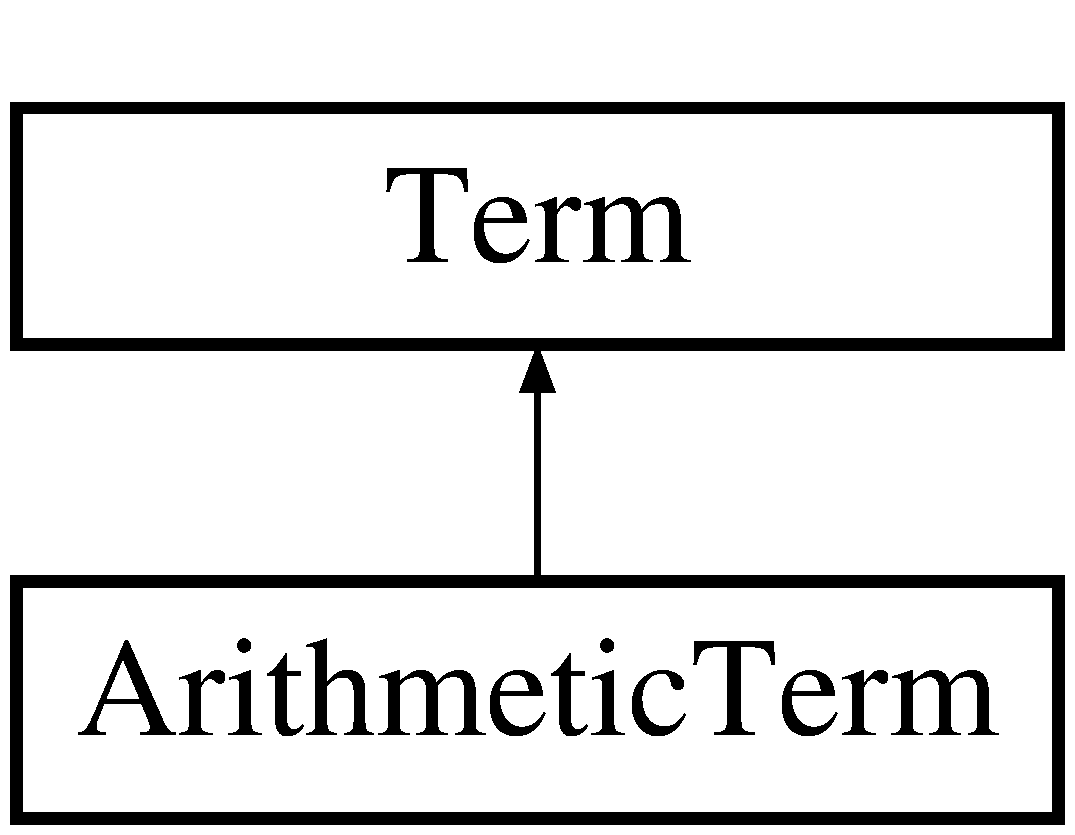
\includegraphics[height=2.000000cm]{classArithmeticTerm}
\end{center}
\end{figure}
\subsection*{\-Public \-Member \-Functions}
\begin{DoxyCompactItemize}
\item 
\hypertarget{classArithmeticTerm_a5933b07779ee448e5f932cfd2b3311ac}{{\bfseries \-Arithmetic\-Term} (const map$<$ \hyperlink{classTerm}{\-Term} $\ast$, long int $>$ \&elems, long int constant)}\label{classArithmeticTerm_a5933b07779ee448e5f932cfd2b3311ac}

\item 
\hypertarget{classArithmeticTerm_add8d90212c068e9feeabde87784f51a5}{const map$<$ \hyperlink{classTerm}{\-Term} $\ast$, long int $>$ \& {\bfseries get\-\_\-elems} ()}\label{classArithmeticTerm_add8d90212c068e9feeabde87784f51a5}

\item 
\hypertarget{classArithmeticTerm_a6c106c116d532bc5b7205696c2c7fc0a}{long int {\bfseries get\-\_\-constant} ()}\label{classArithmeticTerm_a6c106c116d532bc5b7205696c2c7fc0a}

\item 
\hypertarget{classArithmeticTerm_afb75e8dc6b4c4e5c093a48fefc9609c9}{virtual bool {\bfseries operator==} (const \hyperlink{classTerm}{\-Term} \&other)}\label{classArithmeticTerm_afb75e8dc6b4c4e5c093a48fefc9609c9}

\item 
\hypertarget{classArithmeticTerm_a56aa9d6e1a1d6a53a16206d8108695e7}{virtual string {\bfseries to\-\_\-string} ()}\label{classArithmeticTerm_a56aa9d6e1a1d6a53a16206d8108695e7}

\item 
\hypertarget{classArithmeticTerm_a8fdd4308c8e547d1f2ba827f04118190}{virtual \hyperlink{classTerm}{\-Term} $\ast$ {\bfseries substitute} (map$<$ \hyperlink{classTerm}{\-Term} $\ast$, \hyperlink{classTerm}{\-Term} $\ast$ $>$ \&subs)}\label{classArithmeticTerm_a8fdd4308c8e547d1f2ba827f04118190}

\item 
\hypertarget{classArithmeticTerm_ac629594b26985cae31a410b0c271dc25}{long int {\bfseries get\-\_\-gcd} (bool include\-\_\-constant)}\label{classArithmeticTerm_ac629594b26985cae31a410b0c271dc25}

\item 
\hypertarget{classArithmeticTerm_a1b1f59a52e5504ee2a0d5d7aec44199f}{bool {\bfseries has\-\_\-only\-\_\-negative\-\_\-coefficients} ()}\label{classArithmeticTerm_a1b1f59a52e5504ee2a0d5d7aec44199f}

\item 
\hypertarget{classArithmeticTerm_ae4d804551f45cbc75b2f66fa02b60067}{\hyperlink{classTerm}{\-Term} $\ast$ {\bfseries get\-\_\-base} ()}\label{classArithmeticTerm_ae4d804551f45cbc75b2f66fa02b60067}

\end{DoxyCompactItemize}
\subsection*{\-Static \-Public \-Member \-Functions}
\begin{DoxyCompactItemize}
\item 
\hypertarget{classArithmeticTerm_abd2187cdd57a25b0a9f58e1d6f795a01}{static \hyperlink{classTerm}{\-Term} $\ast$ {\bfseries make} (const map$<$ \hyperlink{classTerm}{\-Term} $\ast$, long int $>$ \&elems, long int constant)}\label{classArithmeticTerm_abd2187cdd57a25b0a9f58e1d6f795a01}

\item 
\hypertarget{classArithmeticTerm_a60f57b96887a0425eacde9e2fdfe5542}{static \hyperlink{classTerm}{\-Term} $\ast$ {\bfseries make} (const map$<$ \hyperlink{classTerm}{\-Term} $\ast$, long int $>$ \&elems)}\label{classArithmeticTerm_a60f57b96887a0425eacde9e2fdfe5542}

\item 
\hypertarget{classArithmeticTerm_a0c95ebcd917eda048a0e5e339fc4f555}{static \hyperlink{classArithmeticTerm}{\-Arithmetic\-Term} $\ast$ {\bfseries \-\_\-make} (const map$<$ \hyperlink{classTerm}{\-Term} $\ast$, long int $>$ \&elems, long int constant)}\label{classArithmeticTerm_a0c95ebcd917eda048a0e5e339fc4f555}

\end{DoxyCompactItemize}
\subsection*{\-Protected \-Member \-Functions}
\begin{DoxyCompactItemize}
\item 
\hyperlink{classArithmeticTerm_a47f3b4216d85ab30604544fe967450df}{\-Arithmetic\-Term} (\hyperlink{classTerm}{\-Term} $\ast$t1, long int c1, \hyperlink{classTerm}{\-Term} $\ast$t2, long int c2)
\item 
\hyperlink{classArithmeticTerm_a834c32e850aaaf8fc581f54b37c26151}{\-Arithmetic\-Term} (\hyperlink{classTerm}{\-Term} $\ast$t, long int c)
\end{DoxyCompactItemize}
\subsection*{\-Friends}
\begin{DoxyCompactItemize}
\item 
\hypertarget{classArithmeticTerm_ac98d07dd8f7b70e16ccb9a01abf56b9c}{class {\bfseries boost\-::serialization\-::access}}\label{classArithmeticTerm_ac98d07dd8f7b70e16ccb9a01abf56b9c}

\end{DoxyCompactItemize}


\subsection{\-Constructor \& \-Destructor \-Documentation}
\hypertarget{classArithmeticTerm_a47f3b4216d85ab30604544fe967450df}{\index{\-Arithmetic\-Term@{\-Arithmetic\-Term}!\-Arithmetic\-Term@{\-Arithmetic\-Term}}
\index{\-Arithmetic\-Term@{\-Arithmetic\-Term}!ArithmeticTerm@{\-Arithmetic\-Term}}
\subsubsection[{\-Arithmetic\-Term}]{\setlength{\rightskip}{0pt plus 5cm}\-Arithmetic\-Term\-::\-Arithmetic\-Term (
\begin{DoxyParamCaption}
\item[{{\bf \-Term} $\ast$}]{t1, }
\item[{long int}]{c1, }
\item[{{\bf \-Term} $\ast$}]{t2, }
\item[{long int}]{c2}
\end{DoxyParamCaption}
)\hspace{0.3cm}{\ttfamily  \mbox{[}protected\mbox{]}}}}\label{classArithmeticTerm_a47f3b4216d85ab30604544fe967450df}
c1$\ast$t1 + c2$\ast$t2 \hypertarget{classArithmeticTerm_a834c32e850aaaf8fc581f54b37c26151}{\index{\-Arithmetic\-Term@{\-Arithmetic\-Term}!\-Arithmetic\-Term@{\-Arithmetic\-Term}}
\index{\-Arithmetic\-Term@{\-Arithmetic\-Term}!ArithmeticTerm@{\-Arithmetic\-Term}}
\subsubsection[{\-Arithmetic\-Term}]{\setlength{\rightskip}{0pt plus 5cm}\-Arithmetic\-Term\-::\-Arithmetic\-Term (
\begin{DoxyParamCaption}
\item[{{\bf \-Term} $\ast$}]{t, }
\item[{long int}]{c}
\end{DoxyParamCaption}
)\hspace{0.3cm}{\ttfamily  \mbox{[}protected\mbox{]}}}}\label{classArithmeticTerm_a834c32e850aaaf8fc581f54b37c26151}
t $\ast$ c 

\-The documentation for this class was generated from the following files\-:\begin{DoxyCompactItemize}
\item 
term/\-Arithmetic\-Term.\-h\item 
term/\-Arithmetic\-Term.\-cpp\end{DoxyCompactItemize}

\hypertarget{classBasicHeap}{\section{\-Basic\-Heap$<$ \-Comp $>$ \-Class \-Template \-Reference}
\label{classBasicHeap}\index{\-Basic\-Heap$<$ Comp $>$@{\-Basic\-Heap$<$ Comp $>$}}
}
\subsection*{\-Public \-Member \-Functions}
\begin{DoxyCompactItemize}
\item 
\hypertarget{classBasicHeap_aa3f0020149d0aaf2b42ed3cdafb931ec}{{\bfseries \-Basic\-Heap} (const \-C \&c)}\label{classBasicHeap_aa3f0020149d0aaf2b42ed3cdafb931ec}

\item 
\hypertarget{classBasicHeap_a071a3905e6b0de73a50f2422bee9af27}{int {\bfseries size} () const }\label{classBasicHeap_a071a3905e6b0de73a50f2422bee9af27}

\item 
\hypertarget{classBasicHeap_ac25c1ff043cb5d20b3a01bcc6d68a14f}{bool {\bfseries empty} () const }\label{classBasicHeap_ac25c1ff043cb5d20b3a01bcc6d68a14f}

\item 
\hypertarget{classBasicHeap_a2f91671fe031802ef447a482b7278410}{int {\bfseries operator\mbox{[}$\,$\mbox{]}} (int index) const }\label{classBasicHeap_a2f91671fe031802ef447a482b7278410}

\item 
\hypertarget{classBasicHeap_a9f7018ff27785f5ca02fce999af35c05}{void {\bfseries clear} (bool dealloc=false)}\label{classBasicHeap_a9f7018ff27785f5ca02fce999af35c05}

\item 
\hypertarget{classBasicHeap_a0fb5534dde03067768cdcf19e8391e04}{void {\bfseries insert} (int n)}\label{classBasicHeap_a0fb5534dde03067768cdcf19e8391e04}

\item 
\hypertarget{classBasicHeap_a1dbb1f64bf5bc814515abec8a3468fbb}{int {\bfseries remove\-Min} ()}\label{classBasicHeap_a1dbb1f64bf5bc814515abec8a3468fbb}

\item 
\hypertarget{classBasicHeap_a0e5ce2b16a16ad8a5f33d175cb616a05}{bool {\bfseries heap\-Property} ()}\label{classBasicHeap_a0e5ce2b16a16ad8a5f33d175cb616a05}

\item 
\hypertarget{classBasicHeap_a422eda96fd4ff2f8813767f335f1ae8c}{int {\bfseries getmin} ()}\label{classBasicHeap_a422eda96fd4ff2f8813767f335f1ae8c}

\end{DoxyCompactItemize}
\subsubsection*{template$<$class Comp$>$ class Basic\-Heap$<$ Comp $>$}



\-The documentation for this class was generated from the following file\-:\begin{DoxyCompactItemize}
\item 
sat-\/solver/\-Basic\-Heap.\-h\end{DoxyCompactItemize}

\hypertarget{classbigfraction}{\section{bigfraction \-Class \-Reference}
\label{classbigfraction}\index{bigfraction@{bigfraction}}
}
\subsection*{\-Public \-Member \-Functions}
\begin{DoxyCompactItemize}
\item 
\hypertarget{classbigfraction_ad5d4e003b59fe3f6d6d3932c9dd57bdd}{{\bfseries bigfraction} (\hyperlink{classbignum}{bignum} n)}\label{classbigfraction_ad5d4e003b59fe3f6d6d3932c9dd57bdd}

\item 
\hypertarget{classbigfraction_afb6503630eb947945c1f6149f45be044}{{\bfseries bigfraction} (long int n)}\label{classbigfraction_afb6503630eb947945c1f6149f45be044}

\item 
\hypertarget{classbigfraction_a6ac285151bec865f09757eb5f1a514a9}{{\bfseries bigfraction} (\hyperlink{classbignum}{bignum} n, \hyperlink{classbignum}{bignum} d)}\label{classbigfraction_a6ac285151bec865f09757eb5f1a514a9}

\item 
\hypertarget{classbigfraction_a0ed060536058d1172236a0dbef7e6b9e}{const \hyperlink{classbigfraction}{bigfraction} \& {\bfseries operator=} (\hyperlink{classbigfraction}{bigfraction} other)}\label{classbigfraction_a0ed060536058d1172236a0dbef7e6b9e}

\item 
\hypertarget{classbigfraction_ad705145fa5f7a823e9b83d3489d14ea9}{const \hyperlink{classbigfraction}{bigfraction} \& {\bfseries operator=} (\hyperlink{classbignum}{bignum} other)}\label{classbigfraction_ad705145fa5f7a823e9b83d3489d14ea9}

\item 
\hypertarget{classbigfraction_a7adbab48b1e8ad2696c08e43eb9ce875}{bool {\bfseries is\-\_\-integer} ()}\label{classbigfraction_a7adbab48b1e8ad2696c08e43eb9ce875}

\item 
\hypertarget{classbigfraction_a528fcd88713f443d6a24044f03f523fc}{double {\bfseries to\-\_\-double} ()}\label{classbigfraction_a528fcd88713f443d6a24044f03f523fc}

\item 
\hypertarget{classbigfraction_a9cd1fb05823d7316ea2a56f72d7a4f03}{string {\bfseries to\-\_\-string} ()}\label{classbigfraction_a9cd1fb05823d7316ea2a56f72d7a4f03}

\item 
\hypertarget{classbigfraction_ae873e77f35dcfc84efcbe407a5f2247c}{void {\bfseries operator$\ast$=} (\hyperlink{classbigfraction}{bigfraction} \&other)}\label{classbigfraction_ae873e77f35dcfc84efcbe407a5f2247c}

\item 
\hypertarget{classbigfraction_a569b601736af6ed92841c6887bdbaf37}{void {\bfseries operator$\ast$=} (\hyperlink{classbignum}{bignum} other)}\label{classbigfraction_a569b601736af6ed92841c6887bdbaf37}

\item 
\hypertarget{classbigfraction_a50bc89575e46ab55effb35ea1b5a7afd}{void {\bfseries operator/=} (\hyperlink{classbigfraction}{bigfraction} \&other)}\label{classbigfraction_a50bc89575e46ab55effb35ea1b5a7afd}

\item 
\hypertarget{classbigfraction_a24268457ffd8e80e8d956abe9c19bf8b}{void {\bfseries operator/=} (\hyperlink{classbignum}{bignum} other)}\label{classbigfraction_a24268457ffd8e80e8d956abe9c19bf8b}

\item 
\hypertarget{classbigfraction_a29d101c0715a250b503f91cb6cffe6f0}{void {\bfseries operator+=} (\hyperlink{classbigfraction}{bigfraction} other)}\label{classbigfraction_a29d101c0715a250b503f91cb6cffe6f0}

\item 
\hypertarget{classbigfraction_a5da97ba2887f653dc4ab89538d4e9fee}{void {\bfseries operator+=} (\hyperlink{classbignum}{bignum} other)}\label{classbigfraction_a5da97ba2887f653dc4ab89538d4e9fee}

\item 
\hypertarget{classbigfraction_a32d52fa6ce1c99a84d76c00b0dd5ab88}{void {\bfseries operator-\/=} (\hyperlink{classbigfraction}{bigfraction} other)}\label{classbigfraction_a32d52fa6ce1c99a84d76c00b0dd5ab88}

\item 
\hypertarget{classbigfraction_a8d70f4eaa2d53963ad92aa769f28eebf}{void {\bfseries operator-\/=} (\hyperlink{classbignum}{bignum} other)}\label{classbigfraction_a8d70f4eaa2d53963ad92aa769f28eebf}

\item 
\hypertarget{classbigfraction_acb32b794014044719456ce835d81fa19}{\hyperlink{classbigfraction}{bigfraction} {\bfseries operator$\ast$} (\hyperlink{classbigfraction}{bigfraction} \&other)}\label{classbigfraction_acb32b794014044719456ce835d81fa19}

\item 
\hypertarget{classbigfraction_aadf1ee8de13f0ba98b4dfe9581d41e72}{\hyperlink{classbigfraction}{bigfraction} {\bfseries operator$\ast$} (\hyperlink{classbignum}{bignum} other)}\label{classbigfraction_aadf1ee8de13f0ba98b4dfe9581d41e72}

\item 
\hypertarget{classbigfraction_a3451e5b5d064713882cce0d1d57ffc6c}{\hyperlink{classbigfraction}{bigfraction} {\bfseries operator/} (\hyperlink{classbigfraction}{bigfraction} \&other)}\label{classbigfraction_a3451e5b5d064713882cce0d1d57ffc6c}

\item 
\hypertarget{classbigfraction_abd9d90c7504d41b57efde418f4feb621}{\hyperlink{classbigfraction}{bigfraction} {\bfseries operator/} (\hyperlink{classbignum}{bignum} other)}\label{classbigfraction_abd9d90c7504d41b57efde418f4feb621}

\item 
\hypertarget{classbigfraction_a3ae3d268f0e18dbf3dfd84d631156a45}{\hyperlink{classbigfraction}{bigfraction} {\bfseries operator+} (\hyperlink{classbigfraction}{bigfraction} \&other)}\label{classbigfraction_a3ae3d268f0e18dbf3dfd84d631156a45}

\item 
\hypertarget{classbigfraction_a468a9397f3dcfd26101a3bfdf748f818}{\hyperlink{classbigfraction}{bigfraction} {\bfseries operator+} (\hyperlink{classbignum}{bignum} other)}\label{classbigfraction_a468a9397f3dcfd26101a3bfdf748f818}

\item 
\hypertarget{classbigfraction_a00400c7125bebb2048801d9e93e7a74d}{\hyperlink{classbigfraction}{bigfraction} {\bfseries operator-\/} (\hyperlink{classbigfraction}{bigfraction} \&other)}\label{classbigfraction_a00400c7125bebb2048801d9e93e7a74d}

\item 
\hypertarget{classbigfraction_ae909488d944a82b697567ccf76ccdc12}{\hyperlink{classbigfraction}{bigfraction} {\bfseries operator-\/} (\hyperlink{classbignum}{bignum} other)}\label{classbigfraction_ae909488d944a82b697567ccf76ccdc12}

\item 
\hypertarget{classbigfraction_a140a5e6873c9323f8866e6dcab7173af}{\hyperlink{classbigfraction}{bigfraction} {\bfseries operator-\/} ()}\label{classbigfraction_a140a5e6873c9323f8866e6dcab7173af}

\item 
\hypertarget{classbigfraction_a9985af23b2df78c40ea8858cc1f6cb93}{bool {\bfseries operator==} (\hyperlink{classbigfraction}{bigfraction} other)}\label{classbigfraction_a9985af23b2df78c40ea8858cc1f6cb93}

\item 
\hypertarget{classbigfraction_a9b0ee091ff5e9fc9024d2d1b85b7914d}{bool {\bfseries operator!=} (\hyperlink{classbigfraction}{bigfraction} other)}\label{classbigfraction_a9b0ee091ff5e9fc9024d2d1b85b7914d}

\item 
\hypertarget{classbigfraction_a51adb47a75fcf6da957ed686b8134563}{bool {\bfseries operator!=} (\hyperlink{classbignum}{bignum} other)}\label{classbigfraction_a51adb47a75fcf6da957ed686b8134563}

\item 
\hypertarget{classbigfraction_a745bfc5e7c0460bf6e001c9517cb99ea}{bool {\bfseries operator$<$} (\hyperlink{classbigfraction}{bigfraction} other)}\label{classbigfraction_a745bfc5e7c0460bf6e001c9517cb99ea}

\item 
\hypertarget{classbigfraction_ab7307508e2caa0dfe11fadc18e499822}{bool {\bfseries operator$<$} (\hyperlink{classbignum}{bignum} other)}\label{classbigfraction_ab7307508e2caa0dfe11fadc18e499822}

\item 
\hypertarget{classbigfraction_a81fc7dab0a35a3839fb5e8edba5777a2}{bool {\bfseries operator$<$=} (\hyperlink{classbigfraction}{bigfraction} other)}\label{classbigfraction_a81fc7dab0a35a3839fb5e8edba5777a2}

\item 
\hypertarget{classbigfraction_a713859edec8c1efde237981dc5ca99da}{bool {\bfseries operator$<$=} (\hyperlink{classbignum}{bignum} other)}\label{classbigfraction_a713859edec8c1efde237981dc5ca99da}

\item 
\hypertarget{classbigfraction_a9814a9053be085a3b662766186333e18}{bool {\bfseries operator$>$} (\hyperlink{classbigfraction}{bigfraction} other)}\label{classbigfraction_a9814a9053be085a3b662766186333e18}

\item 
\hypertarget{classbigfraction_aa2ea6344c4991e7008a6bf86c143a7de}{bool {\bfseries operator$>$} (\hyperlink{classbignum}{bignum} other)}\label{classbigfraction_aa2ea6344c4991e7008a6bf86c143a7de}

\item 
\hypertarget{classbigfraction_a94fd50d3ec93326bf09c717c4551c2f2}{bool {\bfseries operator$>$=} (\hyperlink{classbigfraction}{bigfraction} other)}\label{classbigfraction_a94fd50d3ec93326bf09c717c4551c2f2}

\item 
\hypertarget{classbigfraction_ae1e27b46c4cec8702f9d28bafe3a73f0}{bool {\bfseries operator$>$=} (\hyperlink{classbignum}{bignum} other)}\label{classbigfraction_ae1e27b46c4cec8702f9d28bafe3a73f0}

\item 
\hypertarget{classbigfraction_a92cf19988cc969de82148982dda7878a}{\hyperlink{classbignum}{bignum} {\bfseries round\-\_\-down} ()}\label{classbigfraction_a92cf19988cc969de82148982dda7878a}

\item 
\hypertarget{classbigfraction_ae609f16fb3787df33152c70aafa24a38}{\hyperlink{classbignum}{bignum} {\bfseries round\-\_\-up} ()}\label{classbigfraction_ae609f16fb3787df33152c70aafa24a38}

\item 
\hypertarget{classbigfraction_ae9c500a33c81a80fb5e9c53e322ee111}{\hyperlink{classbignum}{bignum} {\bfseries get\-\_\-numerator} ()}\label{classbigfraction_ae9c500a33c81a80fb5e9c53e322ee111}

\item 
\hypertarget{classbigfraction_adc6d2c5ffa0e2bf49410a5dcfc510070}{\hyperlink{classbignum}{bignum} {\bfseries get\-\_\-denominator} ()}\label{classbigfraction_adc6d2c5ffa0e2bf49410a5dcfc510070}

\end{DoxyCompactItemize}
\subsection*{\-Friends}
\begin{DoxyCompactItemize}
\item 
\hypertarget{classbigfraction_a5077af175d27eae5a8f8bd6ed6479f18}{ostream \& {\bfseries operator$<$$<$} (ostream \&os, const \hyperlink{classbigfraction}{bigfraction} \&obj)}\label{classbigfraction_a5077af175d27eae5a8f8bd6ed6479f18}

\end{DoxyCompactItemize}


\-The documentation for this class was generated from the following file\-:\begin{DoxyCompactItemize}
\item 
numeric-\/lib/bigfraction.\-h\end{DoxyCompactItemize}

\hypertarget{classbignum}{\section{bignum \-Class \-Reference}
\label{classbignum}\index{bignum@{bignum}}
}
\subsection*{\-Public \-Member \-Functions}
\begin{DoxyCompactItemize}
\item 
\hypertarget{classbignum_a16c979dcf13417ef6d07123a53664a71}{{\bfseries bignum} (const \hyperlink{classbignum}{bignum} \&other)}\label{classbignum_a16c979dcf13417ef6d07123a53664a71}

\item 
\hypertarget{classbignum_a433de3a42d6200ee42f600bc22552e64}{{\bfseries bignum} (long int i)}\label{classbignum_a433de3a42d6200ee42f600bc22552e64}

\item 
\hypertarget{classbignum_a977eeaee38dbadfd95a9b695714eb4bb}{{\bfseries bignum} (string \&s)}\label{classbignum_a977eeaee38dbadfd95a9b695714eb4bb}

\item 
\hypertarget{classbignum_a5d7254a0767e9aa15d720527caa31d54}{{\bfseries bignum} (const mpz\-\_\-t \&i)}\label{classbignum_a5d7254a0767e9aa15d720527caa31d54}

\item 
\hypertarget{classbignum_ac39efc8fa7c73a1c8c30524ed010e8cb}{const \hyperlink{classbignum}{bignum} \& {\bfseries operator=} (const \hyperlink{classbignum}{bignum} \&other)}\label{classbignum_ac39efc8fa7c73a1c8c30524ed010e8cb}

\item 
\hypertarget{classbignum_ad63321215406159227c662a6ef8daf43}{\hyperlink{classbignum}{bignum} {\bfseries abs} ()}\label{classbignum_ad63321215406159227c662a6ef8daf43}

\item 
\hypertarget{classbignum_ad009bb299f786740933a7eec56642fb3}{bool {\bfseries fits\-\_\-long\-\_\-int} ()}\label{classbignum_ad009bb299f786740933a7eec56642fb3}

\item 
\hypertarget{classbignum_a6a3c9d38bf3a8ce6ba28118e901686c6}{long int {\bfseries to\-\_\-int} ()}\label{classbignum_a6a3c9d38bf3a8ce6ba28118e901686c6}

\item 
\hypertarget{classbignum_a4b44045470c3fbb7c99812edafc740a6}{double {\bfseries to\-\_\-double} ()}\label{classbignum_a4b44045470c3fbb7c99812edafc740a6}

\item 
\hypertarget{classbignum_a2c82d12c4e20bec0bf6ebd2ab5cd7da5}{double {\bfseries divide} (\hyperlink{classbignum}{bignum} \&other)}\label{classbignum_a2c82d12c4e20bec0bf6ebd2ab5cd7da5}

\item 
\hypertarget{classbignum_afdc96d92e3c87e394ade16d690809480}{bool {\bfseries divisible} (\hyperlink{classbignum}{bignum} \&other)}\label{classbignum_afdc96d92e3c87e394ade16d690809480}

\item 
\hypertarget{classbignum_aec60038c4d7ecd8891c40ca95126bc10}{\hyperlink{classbignum}{bignum} {\bfseries compute\-\_\-gcd} (const \hyperlink{classbignum}{bignum} \&other)}\label{classbignum_aec60038c4d7ecd8891c40ca95126bc10}

\item 
\hypertarget{classbignum_a8b732de6597c2062106cc31ec2abc4b5}{\hyperlink{classbignum}{bignum} {\bfseries compute\-\_\-lcm} (const \hyperlink{classbignum}{bignum} \&other)}\label{classbignum_a8b732de6597c2062106cc31ec2abc4b5}

\item 
\hypertarget{classbignum_afb3e0381f468dd324c77c294b1c52770}{\hyperlink{classbignum}{bignum} {\bfseries compute\-\_\-xgcd} (\hyperlink{classbignum}{bignum} \&other, \hyperlink{classbignum}{bignum} \&p, \hyperlink{classbignum}{bignum} \&q)}\label{classbignum_afb3e0381f468dd324c77c294b1c52770}

\item 
\hypertarget{classbignum_a2612bfd43d03554e88cdff205ea7025e}{void {\bfseries operator$\ast$=} (\hyperlink{classbignum}{bignum} \&o1)}\label{classbignum_a2612bfd43d03554e88cdff205ea7025e}

\item 
\hypertarget{classbignum_ab6356b0694d639510e2df5657c65d165}{\hyperlink{classbignum}{bignum} {\bfseries operator$\ast$} (\hyperlink{classbignum}{bignum} o1)}\label{classbignum_ab6356b0694d639510e2df5657c65d165}

\item 
\hypertarget{classbignum_ad5a8b3543b8b82f2d10a69cd1ceda40d}{\hyperlink{classbignum}{bignum} {\bfseries operator\%} (\hyperlink{classbignum}{bignum} o1)}\label{classbignum_ad5a8b3543b8b82f2d10a69cd1ceda40d}

\item 
\hypertarget{classbignum_a85d383868c3102f175f4aba2b685963a}{\hyperlink{classbignum}{bignum} {\bfseries operator/} (\hyperlink{classbignum}{bignum} o1)}\label{classbignum_a85d383868c3102f175f4aba2b685963a}

\item 
\hypertarget{classbignum_adb0611e37e564a1017691a0bf3cbc23e}{\hyperlink{classbignum}{bignum} {\bfseries divexact} (\hyperlink{classbignum}{bignum} \&o1)}\label{classbignum_adb0611e37e564a1017691a0bf3cbc23e}

\item 
\hypertarget{classbignum_a725936f0647ed64888b7bfabdfa6a0a4}{void {\bfseries operator/=} (\hyperlink{classbignum}{bignum} \&o1)}\label{classbignum_a725936f0647ed64888b7bfabdfa6a0a4}

\item 
\hypertarget{classbignum_a48da1062e6ae114ce5c22fc077819953}{void {\bfseries operator+=} (\hyperlink{classbignum}{bignum} o1)}\label{classbignum_a48da1062e6ae114ce5c22fc077819953}

\item 
\hypertarget{classbignum_ae97e69921ac542c6ee739c050ce2ad37}{\hyperlink{classbignum}{bignum} {\bfseries operator+} (\hyperlink{classbignum}{bignum} o1)}\label{classbignum_ae97e69921ac542c6ee739c050ce2ad37}

\item 
\hypertarget{classbignum_aefa3f3353c2eb8546d816b68e6296b9d}{\hyperlink{classbignum}{bignum} {\bfseries operator-\/} (\hyperlink{classbignum}{bignum} o1)}\label{classbignum_aefa3f3353c2eb8546d816b68e6296b9d}

\item 
\hypertarget{classbignum_a033cf97cdb1c84d5869dfb92e4ede8fe}{\hyperlink{classbignum}{bignum} {\bfseries operator-\/} ()}\label{classbignum_a033cf97cdb1c84d5869dfb92e4ede8fe}

\item 
\hypertarget{classbignum_aa613d99028ac70189137f26d019aa619}{void {\bfseries operator-\/=} (\hyperlink{classbignum}{bignum} o1)}\label{classbignum_aa613d99028ac70189137f26d019aa619}

\item 
\hypertarget{classbignum_abb3176518db039b158d6355162494ef6}{bool {\bfseries operator!=} (const \hyperlink{classbignum}{bignum} other)}\label{classbignum_abb3176518db039b158d6355162494ef6}

\item 
\hypertarget{classbignum_ac7be04392d8b2eb6c0854f1787893aa8}{bool {\bfseries operator!=} (long int other)}\label{classbignum_ac7be04392d8b2eb6c0854f1787893aa8}

\item 
\hypertarget{classbignum_a7b18d35498564109ce0ce7fe98545318}{bool {\bfseries operator==} (const \hyperlink{classbignum}{bignum} \&other)}\label{classbignum_a7b18d35498564109ce0ce7fe98545318}

\item 
\hypertarget{classbignum_ac2f7c60cf0aef476384f78542a142413}{bool {\bfseries operator==} (long int i)}\label{classbignum_ac2f7c60cf0aef476384f78542a142413}

\item 
\hypertarget{classbignum_ae4f4dbc03a7090cb369cdf7e8a8b76d8}{bool {\bfseries operator$<$} (const \hyperlink{classbignum}{bignum} \&other) const }\label{classbignum_ae4f4dbc03a7090cb369cdf7e8a8b76d8}

\item 
\hypertarget{classbignum_a5eece074b2f713de3907c97cf5b691c4}{bool {\bfseries operator$<$} (long int i)}\label{classbignum_a5eece074b2f713de3907c97cf5b691c4}

\item 
\hypertarget{classbignum_a02d2efb8a508afe1425cfb94185eb453}{bool {\bfseries operator$<$=} (const \hyperlink{classbignum}{bignum} \&other)}\label{classbignum_a02d2efb8a508afe1425cfb94185eb453}

\item 
\hypertarget{classbignum_af43aca79e2c9a32a68f63f6c5ecdf533}{bool {\bfseries operator$<$=} (long int i)}\label{classbignum_af43aca79e2c9a32a68f63f6c5ecdf533}

\item 
\hypertarget{classbignum_a246a1151b449433723c00ee0d2cbbe5f}{bool {\bfseries operator$>$} (const \hyperlink{classbignum}{bignum} \&other)}\label{classbignum_a246a1151b449433723c00ee0d2cbbe5f}

\item 
\hypertarget{classbignum_a13f091ae485bf085b9b09736b87fc0eb}{bool {\bfseries operator$>$} (long int i)}\label{classbignum_a13f091ae485bf085b9b09736b87fc0eb}

\item 
\hypertarget{classbignum_ace0e9a6071b11db6326f9736d7b59a5c}{bool {\bfseries operator$>$=} (const \hyperlink{classbignum}{bignum} \&other)}\label{classbignum_ace0e9a6071b11db6326f9736d7b59a5c}

\item 
\hypertarget{classbignum_a98cd05681f39cfa5e3848198ac110b7e}{bool {\bfseries operator$>$=} (long int i)}\label{classbignum_a98cd05681f39cfa5e3848198ac110b7e}

\item 
\hypertarget{classbignum_ab8a3fb4a4b1b9f8a606c3c69d5b0b82e}{string {\bfseries to\-\_\-string} ()}\label{classbignum_ab8a3fb4a4b1b9f8a606c3c69d5b0b82e}

\end{DoxyCompactItemize}
\subsection*{\-Static \-Public \-Member \-Functions}
\begin{DoxyCompactItemize}
\item 
\hypertarget{classbignum_a0e4ab887ec8dd76faac83d3af7a7d612}{static bool {\bfseries m\-\_\-overflow} (long int c, long int e)}\label{classbignum_a0e4ab887ec8dd76faac83d3af7a7d612}

\item 
\hypertarget{classbignum_a839abc66d44ee477592c0e588809e016}{static bool {\bfseries a\-\_\-overflow} (long int a, long int b)}\label{classbignum_a839abc66d44ee477592c0e588809e016}

\item 
\hypertarget{classbignum_a6960ba802b03a16ba7f9a0df91ccaaa8}{static long int {\bfseries compute\-\_\-int\-\_\-gcd} (long int \-\_\-a, long int \-\_\-b)}\label{classbignum_a6960ba802b03a16ba7f9a0df91ccaaa8}

\end{DoxyCompactItemize}
\subsection*{\-Public \-Attributes}
\begin{DoxyCompactItemize}
\item 
\hypertarget{classbignum_a8da83f37b8c62026a3ebbf284ac7c991}{\hyperlink{uniondata__type}{data\-\_\-type} {\bfseries data}}\label{classbignum_a8da83f37b8c62026a3ebbf284ac7c991}

\item 
\hypertarget{classbignum_a4940ff4e92feaf5b4a1f0c6eb5a07832}{bool {\bfseries infinite}}\label{classbignum_a4940ff4e92feaf5b4a1f0c6eb5a07832}

\end{DoxyCompactItemize}
\subsection*{\-Friends}
\begin{DoxyCompactItemize}
\item 
\hypertarget{classbignum_a852b7ecc975dd7b8f6e9f293f65af0f6}{ostream \& {\bfseries operator$<$$<$} (ostream \&os, const \hyperlink{classbignum}{bignum} \&obj)}\label{classbignum_a852b7ecc975dd7b8f6e9f293f65af0f6}

\end{DoxyCompactItemize}


\-The documentation for this class was generated from the following file\-:\begin{DoxyCompactItemize}
\item 
numeric-\/lib/bignum.\-h\end{DoxyCompactItemize}

\hypertarget{classBooleanAbstractor}{\section{\-Boolean\-Abstractor \-Class \-Reference}
\label{classBooleanAbstractor}\index{\-Boolean\-Abstractor@{\-Boolean\-Abstractor}}
}
\subsection*{\-Classes}
\begin{DoxyCompactItemize}
\item 
struct {\bfseries edge}
\item 
struct {\bfseries node}
\end{DoxyCompactItemize}
\subsection*{\-Public \-Member \-Functions}
\begin{DoxyCompactItemize}
\item 
\hypertarget{classBooleanAbstractor_ad86f7d3759a8e153d98958fdcd380421}{{\bfseries \-Boolean\-Abstractor} (\hyperlink{classCNode}{\-C\-Node} $\ast$node)}\label{classBooleanAbstractor_ad86f7d3759a8e153d98958fdcd380421}

\item 
\hypertarget{classBooleanAbstractor_a69b8f15a807eee5998f058fb9234b5d4}{\hyperlink{classCNode}{\-C\-Node} $\ast$ {\bfseries get\-\_\-learned\-\_\-implications} ()}\label{classBooleanAbstractor_a69b8f15a807eee5998f058fb9234b5d4}

\end{DoxyCompactItemize}


\-The documentation for this class was generated from the following files\-:\begin{DoxyCompactItemize}
\item 
solver/\-Boolean\-Abstractor.\-h\item 
solver/\-Boolean\-Abstractor.\-cpp\end{DoxyCompactItemize}

\hypertarget{classBooleanVar}{\section{\-Boolean\-Var \-Class \-Reference}
\label{classBooleanVar}\index{\-Boolean\-Var@{\-Boolean\-Var}}
}
\-Inheritance diagram for \-Boolean\-Var\-:\begin{figure}[H]
\begin{center}
\leavevmode
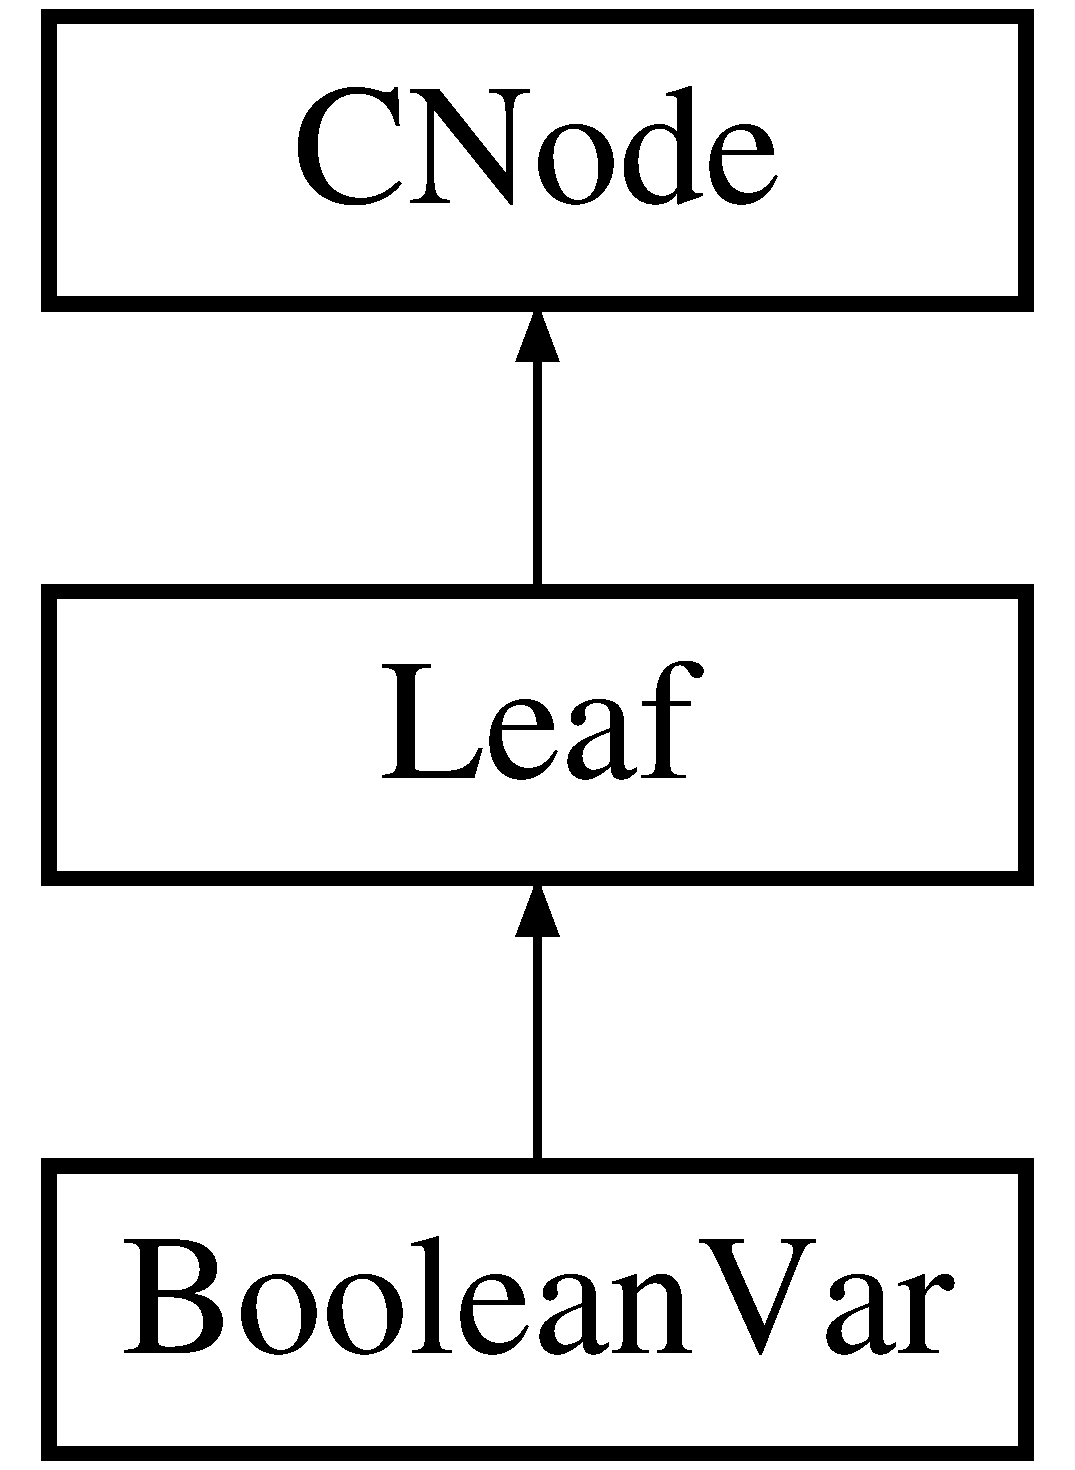
\includegraphics[height=3.000000cm]{classBooleanVar}
\end{center}
\end{figure}
\subsection*{\-Public \-Member \-Functions}
\begin{DoxyCompactItemize}
\item 
\hypertarget{classBooleanVar_af2ffa57fa48de922257c2472b0d39ec4}{unsigned int {\bfseries get\-\_\-id} () const }\label{classBooleanVar_af2ffa57fa48de922257c2472b0d39ec4}

\item 
\hypertarget{classBooleanVar_a8b23054b63232d874f96c58be2221003}{virtual bool {\bfseries operator==} (const \hyperlink{classCNode}{\-C\-Node} \&other)}\label{classBooleanVar_a8b23054b63232d874f96c58be2221003}

\item 
\hypertarget{classBooleanVar_ab2cd6f443e4764db9b31fa3fbeac4b1c}{virtual string {\bfseries to\-\_\-string} ()}\label{classBooleanVar_ab2cd6f443e4764db9b31fa3fbeac4b1c}

\item 
\hypertarget{classBooleanVar_ac50895e6ba40c6f41041eb1da70cf832}{string {\bfseries get\-\_\-name} ()}\label{classBooleanVar_ac50895e6ba40c6f41041eb1da70cf832}

\item 
\hypertarget{classBooleanVar_a375ec1b5e7de706c21134b3b67aac029}{virtual \hyperlink{classCNode}{\-C\-Node} $\ast$ {\bfseries substitute} (map$<$ \hyperlink{classTerm}{\-Term} $\ast$, \hyperlink{classTerm}{\-Term} $\ast$ $>$ \&subs)}\label{classBooleanVar_a375ec1b5e7de706c21134b3b67aac029}

\item 
\hypertarget{classBooleanVar_a867c39319cce9690cbefb312e88ee05f}{\hyperlink{classEqLeaf}{\-Eq\-Leaf} $\ast$ {\bfseries to\-\_\-eqleaf} () const }\label{classBooleanVar_a867c39319cce9690cbefb312e88ee05f}

\end{DoxyCompactItemize}
\subsection*{\-Static \-Public \-Member \-Functions}
\begin{DoxyCompactItemize}
\item 
\hypertarget{classBooleanVar_a174c5223e0b0874c114f7588b3fb1dd8}{static \hyperlink{classBooleanVar}{\-Boolean\-Var} $\ast$ {\bfseries make} ()}\label{classBooleanVar_a174c5223e0b0874c114f7588b3fb1dd8}

\item 
\hypertarget{classBooleanVar_a45d68b4599d3d95beef9194747a92d2c}{static \hyperlink{classBooleanVar}{\-Boolean\-Var} $\ast$ {\bfseries make} (const string \&name)}\label{classBooleanVar_a45d68b4599d3d95beef9194747a92d2c}

\end{DoxyCompactItemize}
\subsection*{\-Protected \-Member \-Functions}
\begin{DoxyCompactItemize}
\item 
\hypertarget{classBooleanVar_a64ca91008decaf02252aa0d8732e8c20}{{\bfseries \-Boolean\-Var} (const string \&name)}\label{classBooleanVar_a64ca91008decaf02252aa0d8732e8c20}

\end{DoxyCompactItemize}
\subsection*{\-Static \-Protected \-Member \-Functions}
\begin{DoxyCompactItemize}
\item 
\hypertarget{classBooleanVar_a26c04fe2ab7dbabfe4f548fed3d7f697}{static void {\bfseries clear} ()}\label{classBooleanVar_a26c04fe2ab7dbabfe4f548fed3d7f697}

\end{DoxyCompactItemize}
\subsection*{\-Friends}
\begin{DoxyCompactItemize}
\item 
\hypertarget{classBooleanVar_a0657a422d4ddc5f4a0ff56931b7d2767}{class {\bfseries \-C\-Node}}\label{classBooleanVar_a0657a422d4ddc5f4a0ff56931b7d2767}

\item 
\hypertarget{classBooleanVar_ac98d07dd8f7b70e16ccb9a01abf56b9c}{class {\bfseries boost\-::serialization\-::access}}\label{classBooleanVar_ac98d07dd8f7b70e16ccb9a01abf56b9c}

\end{DoxyCompactItemize}


\-The documentation for this class was generated from the following files\-:\begin{DoxyCompactItemize}
\item 
cnode/\-Boolean\-Var.\-h\item 
cnode/\-Boolean\-Var.\-cpp\end{DoxyCompactItemize}

\hypertarget{classbvec}{\section{bvec$<$ \-T $>$ \-Class \-Template \-Reference}
\label{classbvec}\index{bvec$<$ T $>$@{bvec$<$ T $>$}}
}
\subsection*{\-Classes}
\begin{DoxyCompactItemize}
\item 
struct {\bfseries \-Vec\-\_\-t}
\end{DoxyCompactItemize}
\subsection*{\-Public \-Member \-Functions}
\begin{DoxyCompactItemize}
\item 
\hypertarget{classbvec_a4239ca77225ee36e4510ed74a08ca0ec}{void {\bfseries clear} (bool dealloc=false)}\label{classbvec_a4239ca77225ee36e4510ed74a08ca0ec}

\item 
\hypertarget{classbvec_a8866e015e816f0060cfc5769c7649529}{{\bfseries altvec} (void)}\label{classbvec_a8866e015e816f0060cfc5769c7649529}

\item 
\hypertarget{classbvec_a622901d76c97a2c9609c11f920fa3c51}{{\bfseries altvec} (int size)}\label{classbvec_a622901d76c97a2c9609c11f920fa3c51}

\item 
\hypertarget{classbvec_a0b8fa7ebcdcdc843606c9a5ef511a8bf}{{\bfseries altvec} (int size, const \-T \&pad)}\label{classbvec_a0b8fa7ebcdcdc843606c9a5ef511a8bf}

\item 
\hypertarget{classbvec_a6e75e1428a4f344cf51713fc4a70ede6}{{\bfseries operator T $\ast$} (void)}\label{classbvec_a6e75e1428a4f344cf51713fc4a70ede6}

\item 
\hypertarget{classbvec_a313e5023735f6727ebe0928edd5438c1}{{\bfseries operator const T $\ast$} (void) const }\label{classbvec_a313e5023735f6727ebe0928edd5438c1}

\item 
\hypertarget{classbvec_a0c26203b7ce42a4d639b191ddebf5acb}{int {\bfseries size} (void) const }\label{classbvec_a0c26203b7ce42a4d639b191ddebf5acb}

\item 
\hypertarget{classbvec_a19268a2dc6d4526fb38eafd1228e0646}{void {\bfseries pop} (void)}\label{classbvec_a19268a2dc6d4526fb38eafd1228e0646}

\item 
\hypertarget{classbvec_a5d555ed303cf0be27417fd89ac55cb33}{void {\bfseries push} (const \-T \&elem)}\label{classbvec_a5d555ed303cf0be27417fd89ac55cb33}

\item 
\hypertarget{classbvec_a5a6768d414be10ec8ad7dcc675e63e3a}{void {\bfseries push} ()}\label{classbvec_a5a6768d414be10ec8ad7dcc675e63e3a}

\item 
\hypertarget{classbvec_ad85ed6e03f4825856951cfaeebe1497b}{void {\bfseries shrink} (int nelems)}\label{classbvec_ad85ed6e03f4825856951cfaeebe1497b}

\item 
\hypertarget{classbvec_afaa1f15e57166b74f9cd4754b7e24310}{void {\bfseries shrink\-\_\-} (int nelems)}\label{classbvec_afaa1f15e57166b74f9cd4754b7e24310}

\item 
\hypertarget{classbvec_a3466c2d0f0878b464567950714c7666c}{void {\bfseries grow\-To} (int size)}\label{classbvec_a3466c2d0f0878b464567950714c7666c}

\item 
\hypertarget{classbvec_af51a7824e3937ad8813b1df7c98e4233}{void {\bfseries grow\-To} (int size, const \-T \&pad)}\label{classbvec_af51a7824e3937ad8813b1df7c98e4233}

\item 
\hypertarget{classbvec_a58d27822f707ef997351ca121ed87dc3}{void {\bfseries capacity} (int size)}\label{classbvec_a58d27822f707ef997351ca121ed87dc3}

\item 
\hypertarget{classbvec_a84cb9fb3aa5db961d2fcb806a78fd4b8}{const \-T \& {\bfseries last} (void) const }\label{classbvec_a84cb9fb3aa5db961d2fcb806a78fd4b8}

\item 
\hypertarget{classbvec_ac5fb612cb7050f3fe723065babc396f5}{\-T \& {\bfseries last} (void)}\label{classbvec_ac5fb612cb7050f3fe723065babc396f5}

\item 
\hypertarget{classbvec_aa4866e84560978edf461c9a9abb21128}{const \-T \& {\bfseries operator\mbox{[}$\,$\mbox{]}} (int index) const }\label{classbvec_aa4866e84560978edf461c9a9abb21128}

\item 
\hypertarget{classbvec_a52486ad5c60b8584bfb64e3e3151c5af}{\-T \& {\bfseries operator\mbox{[}$\,$\mbox{]}} (int index)}\label{classbvec_a52486ad5c60b8584bfb64e3e3151c5af}

\item 
\hypertarget{classbvec_a1b3fb5fde0a343984e57b9ac35d3c32f}{void {\bfseries copy\-To} (altvec$<$ \-T $>$ \&copy) const }\label{classbvec_a1b3fb5fde0a343984e57b9ac35d3c32f}

\item 
\hypertarget{classbvec_a32419717f610e60d0bee7d55e320467f}{void {\bfseries move\-To} (altvec$<$ \-T $>$ \&dest)}\label{classbvec_a32419717f610e60d0bee7d55e320467f}

\end{DoxyCompactItemize}
\subsubsection*{template$<$class T$>$ class bvec$<$ T $>$}



\-The documentation for this class was generated from the following file\-:\begin{DoxyCompactItemize}
\item 
sat-\/solver/\-Boxed\-Vec.\-h\end{DoxyCompactItemize}

\hypertarget{classClause}{\section{\-Clause \-Class \-Reference}
\label{classClause}\index{\-Clause@{\-Clause}}
}
\subsection*{\-Public \-Member \-Functions}
\begin{DoxyCompactItemize}
\item 
\hypertarget{classClause_a36f5d7a9f0d9ec42766c17fbf1130003}{{\bfseries \-Clause} (\hyperlink{classCNode}{\-C\-Node} $\ast$node)}\label{classClause_a36f5d7a9f0d9ec42766c17fbf1130003}

\item 
\hypertarget{classClause_a6b06a55baada1e60a6d7e4a7a299f61b}{bool {\bfseries subsumes} (\hyperlink{classClause}{\-Clause} \&other)}\label{classClause_a6b06a55baada1e60a6d7e4a7a299f61b}

\item 
\hypertarget{classClause_a7db0ab185dcf82f240d08a651b4f0a93}{bool {\bfseries drop\-\_\-clause} ()}\label{classClause_a7db0ab185dcf82f240d08a651b4f0a93}

\item 
\hypertarget{classClause_a2f75f195619ff5e211fc347f5505a963}{string {\bfseries to\-\_\-string} (string c)}\label{classClause_a2f75f195619ff5e211fc347f5505a963}

\item 
\hypertarget{classClause_a966d45e9babc2d296eac53a0b3721f06}{\hyperlink{classCNode}{\-C\-Node} $\ast$ {\bfseries to\-\_\-cnode} (bool use\-\_\-and=true)}\label{classClause_a966d45e9babc2d296eac53a0b3721f06}

\item 
\hypertarget{classClause_a50d3423d651ccb8572608b87983478b2}{void {\bfseries denest} (map$<$ \hyperlink{classTerm}{\-Term} $\ast$, \hyperlink{classTerm}{\-Term} $\ast$ $>$ $\ast$denestings=\-N\-U\-L\-L)}\label{classClause_a50d3423d651ccb8572608b87983478b2}

\end{DoxyCompactItemize}
\subsection*{\-Public \-Attributes}
\begin{DoxyCompactItemize}
\item 
\hypertarget{classClause_adadc497c5bbdb64f2978fad4db613ff0}{set$<$ \hyperlink{classEqLeaf}{\-Eq\-Leaf} $\ast$ $>$ {\bfseries pos\-\_\-eq}}\label{classClause_adadc497c5bbdb64f2978fad4db613ff0}

\item 
\hypertarget{classClause_a7ff2197334cae1e18d3fba03001577d0}{set$<$ \hyperlink{classEqLeaf}{\-Eq\-Leaf} $\ast$ $>$ {\bfseries neg\-\_\-eq}}\label{classClause_a7ff2197334cae1e18d3fba03001577d0}

\item 
\hypertarget{classClause_a1e26ec2f623668688f37ca16324b2d07}{set$<$ \hyperlink{classILPLeaf}{\-I\-L\-P\-Leaf} $\ast$ $>$ {\bfseries pos\-\_\-ilp}}\label{classClause_a1e26ec2f623668688f37ca16324b2d07}

\item 
\hypertarget{classClause_af4a320a17a612b8120289fb3e18a9149}{set$<$ \hyperlink{classILPLeaf}{\-I\-L\-P\-Leaf} $\ast$ $>$ {\bfseries neg\-\_\-ilp}}\label{classClause_af4a320a17a612b8120289fb3e18a9149}

\item 
\hypertarget{classClause_a98ea135fa9c9a15f968f24c0cdcdd0f7}{set$<$ \hyperlink{classModLeaf}{\-Mod\-Leaf} $\ast$ $>$ {\bfseries pos\-\_\-mod}}\label{classClause_a98ea135fa9c9a15f968f24c0cdcdd0f7}

\item 
\hypertarget{classClause_a5c718ef3a32ccd15a8b21386a75e5ce8}{set$<$ \hyperlink{classModLeaf}{\-Mod\-Leaf} $\ast$ $>$ {\bfseries neg\-\_\-mod}}\label{classClause_a5c718ef3a32ccd15a8b21386a75e5ce8}

\item 
\hypertarget{classClause_a96bf796b56ff0bc9213292973366be52}{set$<$ \hyperlink{classQuantifiedLeaf}{\-Quantified\-Leaf} $\ast$ $>$ {\bfseries pos\-\_\-universal}}\label{classClause_a96bf796b56ff0bc9213292973366be52}

\item 
\hypertarget{classClause_a64f7177e40c247d49fd7515dcc5e47d1}{set$<$ \hyperlink{classQuantifiedLeaf}{\-Quantified\-Leaf} $\ast$ $>$ {\bfseries neg\-\_\-universal}}\label{classClause_a64f7177e40c247d49fd7515dcc5e47d1}

\item 
\hypertarget{classClause_ae8c2e0ecbfdab63b1aeab80429eadd55}{map$<$ \hyperlink{classTerm}{\-Term} $\ast$, \hyperlink{classTerm}{\-Term} $\ast$ $>$ {\bfseries reverse\-\_\-denestings}}\label{classClause_ae8c2e0ecbfdab63b1aeab80429eadd55}

\end{DoxyCompactItemize}


\-The documentation for this class was generated from the following files\-:\begin{DoxyCompactItemize}
\item 
solver/\-Clause.\-h\item 
solver/\-Clause.\-cpp\end{DoxyCompactItemize}

\hypertarget{classClauseSolve}{\section{\-Clause\-Solve \-Class \-Reference}
\label{classClauseSolve}\index{\-Clause\-Solve@{\-Clause\-Solve}}
}
\subsection*{\-Classes}
\begin{DoxyCompactItemize}
\item 
struct {\bfseries history\-\_\-elem}
\end{DoxyCompactItemize}
\subsection*{\-Public \-Member \-Functions}
\begin{DoxyCompactItemize}
\item 
\hypertarget{classClauseSolve_a7594792761da2b9e818f31fced46676d}{{\bfseries \-Clause\-Solve} (\hyperlink{classCNode}{\-C\-Node} $\ast$node, map$<$ \hyperlink{classTerm}{\-Term} $\ast$, \hyperlink{classSatValue}{\-Sat\-Value} $>$ $\ast$assignments=\-N\-U\-L\-L)}\label{classClauseSolve_a7594792761da2b9e818f31fced46676d}

\item 
\hypertarget{classClauseSolve_aceb5efa9b6af4cc28fb4e890d65cfd71}{{\bfseries \-Clause\-Solve} (\hyperlink{classClause}{\-Clause} $\ast$clause, map$<$ \hyperlink{classTerm}{\-Term} $\ast$, \hyperlink{classSatValue}{\-Sat\-Value} $>$ $\ast$assignments=\-N\-U\-L\-L)}\label{classClauseSolve_aceb5efa9b6af4cc28fb4e890d65cfd71}

\item 
\hypertarget{classClauseSolve_a1de13db3dc2a960d001281206418eea9}{bool {\bfseries is\-\_\-sat} ()}\label{classClauseSolve_a1de13db3dc2a960d001281206418eea9}

\item 
\hypertarget{classClauseSolve_a6d2d6816c8f799062d315ad12a86aacf}{void {\bfseries print\-\_\-stats} ()}\label{classClauseSolve_a6d2d6816c8f799062d315ad12a86aacf}

\end{DoxyCompactItemize}
\subsection*{\-Friends}
\begin{DoxyCompactItemize}
\item 
\hypertarget{classClauseSolve_ace1aed02802f62c643a37b8a67e67bee}{class {\bfseries \-Interaction\-Manager}}\label{classClauseSolve_ace1aed02802f62c643a37b8a67e67bee}

\item 
\hypertarget{classClauseSolve_a16b09189cdaf88044be661f54a1313a7}{class {\bfseries \-Query\-Comparator}}\label{classClauseSolve_a16b09189cdaf88044be661f54a1313a7}

\item 
\hypertarget{classClauseSolve_aa97b604ea37345da6b2414f0892e2664}{class {\bfseries \-Variable\-Eliminator}}\label{classClauseSolve_aa97b604ea37345da6b2414f0892e2664}

\item 
\hypertarget{classClauseSolve_ac354b9f1700ae74fadac1ee9efad4475}{class {\bfseries \-Equality\-Finder}}\label{classClauseSolve_ac354b9f1700ae74fadac1ee9efad4475}

\end{DoxyCompactItemize}


\-The documentation for this class was generated from the following files\-:\begin{DoxyCompactItemize}
\item 
solver/\-Clause\-Solve.\-h\item 
solver/\-Clause\-Solve.\-cpp\end{DoxyCompactItemize}

\hypertarget{classCNF}{\section{\-C\-N\-F \-Class \-Reference}
\label{classCNF}\index{\-C\-N\-F@{\-C\-N\-F}}
}
\subsection*{\-Public \-Member \-Functions}
\begin{DoxyCompactItemize}
\item 
\hypertarget{classCNF_abc6608d3e61a97f5a713ec79a2d5a78e}{{\bfseries \-C\-N\-F} (\hyperlink{classCNode}{\-C\-Node} $\ast$node, \hyperlink{classminisat_1_1Solver}{minisat\-::\-Solver} \&s)}\label{classCNF_abc6608d3e61a97f5a713ec79a2d5a78e}

\item 
\hypertarget{classCNF_a0716cf08ea2eca3bc713c1e1fe76cfc5}{\hyperlink{classvec}{vec}$<$ \hyperlink{classminisat_1_1Lit}{minisat\-::\-Lit} $>$ $\ast$ {\bfseries add\-\_\-clause} (\hyperlink{classCNode}{\-C\-Node} $\ast$clause, \hyperlink{classminisat_1_1Solver}{minisat\-::\-Solver} \&s)}\label{classCNF_a0716cf08ea2eca3bc713c1e1fe76cfc5}

\item 
\hypertarget{classCNF_ae0d4f72d022b070f57f1b2c252a61b58}{void {\bfseries and\-\_\-cnf} (\hyperlink{classCNF}{\-C\-N\-F} \&other)}\label{classCNF_ae0d4f72d022b070f57f1b2c252a61b58}

\item 
\hypertarget{classCNF_a2be099608573de21156b5dfc54042485}{string {\bfseries to\-\_\-string} ()}\label{classCNF_a2be099608573de21156b5dfc54042485}

\item 
\hypertarget{classCNF_aa353261cc8a24c6940787c662c18c7cd}{set$<$ \hyperlink{classvec}{vec}$<$ \hyperlink{classminisat_1_1Lit}{minisat\-::\-Lit} $>$ $\ast$ $>$ \& {\bfseries get\-\_\-cnf} ()}\label{classCNF_aa353261cc8a24c6940787c662c18c7cd}

\item 
\hypertarget{classCNF_aac7fc5db637bc524750a3ead50790085}{\hyperlink{classLeaf}{\-Leaf} $\ast$ {\bfseries get\-\_\-leaf\-\_\-from\-\_\-literal} (minisat\-::\-Var l)}\label{classCNF_aac7fc5db637bc524750a3ead50790085}

\item 
\hypertarget{classCNF_ae7ee11aa4cbfbf6d95a0ceb6877f6f79}{void {\bfseries and\-\_\-node} (\hyperlink{classCNode}{\-C\-Node} $\ast$node, \hyperlink{classminisat_1_1Solver}{minisat\-::\-Solver} \&s)}\label{classCNF_ae7ee11aa4cbfbf6d95a0ceb6877f6f79}

\item 
\hypertarget{classCNF_a29b94db8b9b26e870a0ee92a3890c80f}{map$<$ minisat\-::\-Var, \hyperlink{classCNode}{\-C\-Node} $\ast$ $>$ \& {\bfseries get\-\_\-var\-\_\-to\-\_\-node\-\_\-map} ()}\label{classCNF_a29b94db8b9b26e870a0ee92a3890c80f}

\end{DoxyCompactItemize}


\-The documentation for this class was generated from the following files\-:\begin{DoxyCompactItemize}
\item 
solver/\-C\-N\-F.\-h\item 
solver/\-C\-N\-F.\-cpp\end{DoxyCompactItemize}

\hypertarget{classCNode}{\section{\-C\-Node \-Class \-Reference}
\label{classCNode}\index{\-C\-Node@{\-C\-Node}}
}
\-Inheritance diagram for \-C\-Node\-:\begin{figure}[H]
\begin{center}
\leavevmode
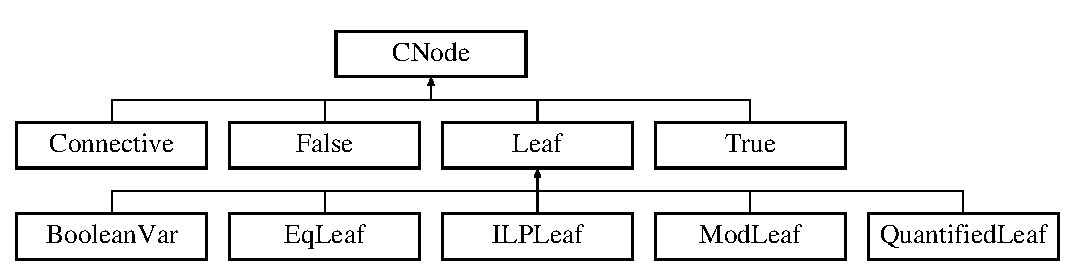
\includegraphics[height=3.000000cm]{classCNode}
\end{center}
\end{figure}
\subsection*{\-Classes}
\begin{DoxyCompactItemize}
\item 
struct {\bfseries refactor\-\_\-lessthan}
\end{DoxyCompactItemize}
\subsection*{\-Public \-Member \-Functions}
\begin{DoxyCompactItemize}
\item 
\hypertarget{classCNode_a160d72ba87c7daee766f2a4386a25e48}{\hyperlink{classCNode}{\-C\-Node} $\ast$ {\bfseries get\-\_\-simplification} (simplification\-\_\-level min\-\_\-level)}\label{classCNode_a160d72ba87c7daee766f2a4386a25e48}

\item 
\hypertarget{classCNode_abc5894d98b671e977d7659b42fd65176}{void {\bfseries set\-\_\-simplification} (\hyperlink{classCNode}{\-C\-Node} $\ast$simplified\-\_\-node, simplification\-\_\-level level)}\label{classCNode_abc5894d98b671e977d7659b42fd65176}

\item 
\hypertarget{classCNode_ae815e6683207015e30dcd66104e02434}{\hyperlink{classCNode}{\-C\-Node} $\ast$ {\bfseries refactor} ()}\label{classCNode_ae815e6683207015e30dcd66104e02434}

\item 
\hypertarget{classCNode_a890c35e430066c0c1e88e9918f9cafca}{\hyperlink{classCNode}{\-C\-Node} $\ast$ {\bfseries make\-\_\-canonical} ()}\label{classCNode_a890c35e430066c0c1e88e9918f9cafca}

\item 
\hypertarget{classCNode_a7765b18fe194fb0fb07e9bdf98d70889}{bool {\bfseries check\-\_\-canonical} ()}\label{classCNode_a7765b18fe194fb0fb07e9bdf98d70889}

\item 
\hypertarget{classCNode_a5e5ce9b83eea3a92484e1ba930067580}{\hyperlink{classCNode}{\-C\-Node} $\ast$ {\bfseries get\-\_\-attribute\-\_\-constraints} ()}\label{classCNode_a5e5ce9b83eea3a92484e1ba930067580}

\item 
\hypertarget{classCNode_a2a8156e96d3621d58bfe43cc91d7aa8a}{virtual \hyperlink{classCNode}{\-C\-Node} $\ast$ {\bfseries substitute} (map$<$ \hyperlink{classTerm}{\-Term} $\ast$, \hyperlink{classTerm}{\-Term} $\ast$ $>$ \&subs)=0}\label{classCNode_a2a8156e96d3621d58bfe43cc91d7aa8a}

\item 
\hypertarget{classCNode_aaca668f2d986e480599bd69adeeeea39}{\hyperlink{classCNode}{\-C\-Node} $\ast$ {\bfseries substitute} (\hyperlink{classTerm}{\-Term} $\ast$($\ast$sub\-\_\-func)(\hyperlink{classTerm}{\-Term} $\ast$t))}\label{classCNode_aaca668f2d986e480599bd69adeeeea39}

\item 
\hypertarget{classCNode_aa6c73cd96659f601a7477f1faad7affc}{\hyperlink{classCNode}{\-C\-Node} $\ast$ {\bfseries substitute} (\hyperlink{classTerm}{\-Term} $\ast$t1, \hyperlink{classTerm}{\-Term} $\ast$t2)}\label{classCNode_aa6c73cd96659f601a7477f1faad7affc}

\item 
\hypertarget{classCNode_a05a2e1e7856e0dd08bfcdbeb931b3314}{\hyperlink{classCNode}{\-C\-Node} $\ast$ {\bfseries substitute} (\hyperlink{classTerm}{\-Term} $\ast$($\ast$sub\-\_\-func)(\hyperlink{classTerm}{\-Term} $\ast$t, void $\ast$data), void $\ast$my\-\_\-data)}\label{classCNode_a05a2e1e7856e0dd08bfcdbeb931b3314}

\item 
\hypertarget{classCNode_a1d307f77bff582d014e8744f01dd3590}{\hyperlink{classCNode}{\-C\-Node} $\ast$ {\bfseries substitute} (map$<$ \hyperlink{classCNode}{\-C\-Node} $\ast$, \hyperlink{classCNode}{\-C\-Node} $\ast$ $>$ \&subs)}\label{classCNode_a1d307f77bff582d014e8744f01dd3590}

\item 
\hypertarget{classCNode_aa05994b70eb79ef5e710d9701915ddea}{cnode\-\_\-type {\bfseries get\-\_\-type} () const }\label{classCNode_aa05994b70eb79ef5e710d9701915ddea}

\item 
\hypertarget{classCNode_a7aa6de21240ebf7cc484eb4758c99d77}{virtual bool {\bfseries operator==} (const \hyperlink{classCNode}{\-C\-Node} \&other)=0}\label{classCNode_a7aa6de21240ebf7cc484eb4758c99d77}

\item 
\hypertarget{classCNode_a306eb6bd36cdd5ae4d792b6707bb638c}{virtual string {\bfseries to\-\_\-string} ()=0}\label{classCNode_a306eb6bd36cdd5ae4d792b6707bb638c}

\item 
\hypertarget{classCNode_a44d94a128de88cbe26383459cc4473b3}{string {\bfseries to\-\_\-prefix\-\_\-notation} ()}\label{classCNode_a44d94a128de88cbe26383459cc4473b3}

\item 
\hypertarget{classCNode_a27715dd1f5669edcb611e50504043b7f}{bool {\bfseries is\-\_\-leaf} () const }\label{classCNode_a27715dd1f5669edcb611e50504043b7f}

\item 
\hypertarget{classCNode_a85bb30e59b95ddcf540d95c343496d35}{bool {\bfseries is\-\_\-literal} () const }\label{classCNode_a85bb30e59b95ddcf540d95c343496d35}

\item 
\hypertarget{classCNode_a7160054b9009ac754adf939fcede2c06}{bool {\bfseries is\-\_\-connective} () const }\label{classCNode_a7160054b9009ac754adf939fcede2c06}

\item 
\hypertarget{classCNode_a9f8ba18507cf325f16c27aefb2f08144}{bool {\bfseries is\-\_\-conjunct} () const }\label{classCNode_a9f8ba18507cf325f16c27aefb2f08144}

\item 
\hypertarget{classCNode_a844e27e25a8922209ff1692ae6176dc5}{bool {\bfseries is\-\_\-disjunct} () const }\label{classCNode_a844e27e25a8922209ff1692ae6176dc5}

\item 
\hypertarget{classCNode_a9cb25629fb582727223b4f7375229b2a}{bool {\bfseries has\-\_\-quantifier} () const }\label{classCNode_a9cb25629fb582727223b4f7375229b2a}

\item 
\hypertarget{classCNode_aeba7734a7bf98f7dd0c2555854cb7b77}{bool {\bfseries contains\-\_\-inequality} ()}\label{classCNode_aeba7734a7bf98f7dd0c2555854cb7b77}

\item 
\hypertarget{classCNode_ab501fd73558903d8acf3929edf125db1}{bool {\bfseries is\-\_\-constant} () const }\label{classCNode_ab501fd73558903d8acf3929edf125db1}

\item 
\hypertarget{classCNode_a35776e5a7020e14f06e2538f3ddb949b}{size\-\_\-t {\bfseries hash\-\_\-code} ()}\label{classCNode_a35776e5a7020e14f06e2538f3ddb949b}

\item 
\hypertarget{classCNode_acb109c93cc7db248648a32f9edc7004c}{void {\bfseries get\-\_\-vars} (set$<$ string $>$ \&vars)}\label{classCNode_acb109c93cc7db248648a32f9edc7004c}

\item 
\hypertarget{classCNode_a67e5a06823614885686a1b4742eeafec}{void {\bfseries get\-\_\-vars} (set$<$ int $>$ \&vars)}\label{classCNode_a67e5a06823614885686a1b4742eeafec}

\item 
\hypertarget{classCNode_a68ada4c5f7820ef613f2c0e28ec0ac10}{void {\bfseries get\-\_\-vars} (set$<$ \hyperlink{classTerm}{\-Term} $\ast$ $>$ \&vars)}\label{classCNode_a68ada4c5f7820ef613f2c0e28ec0ac10}

\item 
\hypertarget{classCNode_aa0a9793c7cc5d1f91c85e00e1138a4f8}{bool {\bfseries contains\-\_\-var} (int var\-\_\-id)}\label{classCNode_aa0a9793c7cc5d1f91c85e00e1138a4f8}

\item 
\hypertarget{classCNode_a10164153f252916e456e055c316d47a5}{bool {\bfseries contains\-\_\-term} (\hyperlink{classTerm}{\-Term} $\ast$t)}\label{classCNode_a10164153f252916e456e055c316d47a5}

\item 
\hypertarget{classCNode_a156bf58e215ebbdaac842f00b5e63918}{bool {\bfseries contains\-\_\-term} (set$<$ \hyperlink{classTerm}{\-Term} $\ast$ $>$ \&terms)}\label{classCNode_a156bf58e215ebbdaac842f00b5e63918}

\item 
\hypertarget{classCNode_a58ba20cf8663d331e3d673663aaaea3a}{\hyperlink{classCNode}{\-C\-Node} $\ast$ {\bfseries rename\-\_\-variable} (int old\-\_\-var\-\_\-id, int new\-\_\-var\-\_\-id)}\label{classCNode_a58ba20cf8663d331e3d673663aaaea3a}

\item 
\hypertarget{classCNode_aa25a2fba15e7aeb52174407a93aa4896}{\hyperlink{classCNode}{\-C\-Node} $\ast$ {\bfseries rename\-\_\-variables} (map$<$ int, int $>$ \&replacements)}\label{classCNode_aa25a2fba15e7aeb52174407a93aa4896}

\item 
\hypertarget{classCNode_a4e8f06ac7ad1d2bda0bb78fccc74d2aa}{void {\bfseries get\-\_\-nested\-\_\-terms} (set$<$ \hyperlink{classTerm}{\-Term} $\ast$ $>$ \&terms, bool include\-\_\-function\-\_\-subterms, bool include\-\_\-constants=true)}\label{classCNode_a4e8f06ac7ad1d2bda0bb78fccc74d2aa}

\item 
\hypertarget{classCNode_af8d20473d1835212ab5d5cfd1f4773af}{\hyperlink{classCNode}{\-C\-Node} $\ast$ {\bfseries add\-\_\-attributes} (set$<$ \hyperlink{classTerm}{\-Term} $\ast$ $>$ $\ast$which\-\_\-terms=\-N\-U\-L\-L)}\label{classCNode_af8d20473d1835212ab5d5cfd1f4773af}

\item 
\hypertarget{classCNode_a2b96f8c546f271a2d8843369fca71cfc}{\hyperlink{classTerm}{\-Term} $\ast$ {\bfseries contains\-\_\-term\-\_\-equality} (\hyperlink{classTerm}{\-Term} $\ast$t)}\label{classCNode_a2b96f8c546f271a2d8843369fca71cfc}

\item 
\hypertarget{classCNode_a1cc071b0fb85fc2c20fb3d502fdb5525}{void {\bfseries collect\-\_\-term\-\_\-equalities} (\hyperlink{classTerm}{\-Term} $\ast$t, set$<$ \hyperlink{classTerm}{\-Term} $\ast$ $>$ \&eqs)}\label{classCNode_a1cc071b0fb85fc2c20fb3d502fdb5525}

\item 
\hypertarget{classCNode_af1397150f71cdaeb70178322fdbb668f}{\hyperlink{classCNode}{\-C\-Node} $\ast$ {\bfseries replace\-\_\-leaves\-\_\-containing\-\_\-term} (\hyperlink{classTerm}{\-Term} $\ast$t, \hyperlink{classCNode}{\-C\-Node} $\ast$replacement)}\label{classCNode_af1397150f71cdaeb70178322fdbb668f}

\item 
\hypertarget{classCNode_a515775fb290af1c3592e607caa57641a}{\hyperlink{classCNode}{\-C\-Node} $\ast$ {\bfseries replace} (\hyperlink{classCNode}{\-C\-Node} $\ast$orig, \hyperlink{classCNode}{\-C\-Node} $\ast$replacement)}\label{classCNode_a515775fb290af1c3592e607caa57641a}

\item 
\hypertarget{classCNode_a91b43fd7e7aea2c5b0f05aece82b97d1}{int {\bfseries num\-\_\-leaves\-\_\-containing\-\_\-term} (\hyperlink{classTerm}{\-Term} $\ast$t)}\label{classCNode_a91b43fd7e7aea2c5b0f05aece82b97d1}

\item 
\hypertarget{classCNode_ab76c3b160eaf38f42660f9b7c58d075c}{void {\bfseries get\-\_\-all\-\_\-literals} (set$<$ \hyperlink{classCNode}{\-C\-Node} $\ast$ $>$ \&literals)}\label{classCNode_ab76c3b160eaf38f42660f9b7c58d075c}

\item 
\hypertarget{classCNode_afca74e7e830916abcc11e16c71a6f38e}{void {\bfseries get\-\_\-all\-\_\-leaves} (set$<$ \hyperlink{classCNode}{\-C\-Node} $\ast$ $>$ \&leaves)}\label{classCNode_afca74e7e830916abcc11e16c71a6f38e}

\item 
\hypertarget{classCNode_aa8f4b9b400fc9d2c5db0d81e63541522}{void {\bfseries get\-\_\-literals\-\_\-containing\-\_\-term} (\hyperlink{classTerm}{\-Term} $\ast$t, set$<$ \hyperlink{classCNode}{\-C\-Node} $\ast$ $>$ \&leaves)}\label{classCNode_aa8f4b9b400fc9d2c5db0d81e63541522}

\item 
\hypertarget{classCNode_ab4aff7ed0f90db7af3a89f37fd8f0c55}{\hyperlink{classCNode}{\-C\-Node} $\ast$ {\bfseries fold\-\_\-negated\-\_\-ilps} ()}\label{classCNode_ab4aff7ed0f90db7af3a89f37fd8f0c55}

\item 
\hypertarget{classCNode_ab1bdf2d02417c0e468cf30ba73c9fe4a}{int {\bfseries get\-\_\-size} ()}\label{classCNode_ab1bdf2d02417c0e468cf30ba73c9fe4a}

\item 
\hypertarget{classCNode_ab333c2f0b29753e4f627ce5576d317e0}{\hyperlink{classCNode}{\-C\-Node} $\ast$ {\bfseries evaluate\-\_\-assignment} (map$<$ \hyperlink{classTerm}{\-Term} $\ast$, \hyperlink{classSatValue}{\-Sat\-Value} $>$ \&assignment)}\label{classCNode_ab333c2f0b29753e4f627ce5576d317e0}

\item 
\hypertarget{classCNode_aff2111bfcd019bc2f7224d44b9482eb6}{\hyperlink{classCNode}{\-C\-Node} $\ast$ {\bfseries evaluate\-\_\-assignment} (map$<$ \hyperlink{classCNode}{\-C\-Node} $\ast$, bool $>$ \&assignments)}\label{classCNode_aff2111bfcd019bc2f7224d44b9482eb6}

\item 
\hypertarget{classCNode_a44103c28feda4d67c50b0f91160b1086}{void {\bfseries get\-\_\-all\-\_\-fun\-\_\-ids} (set$<$ int $>$ \&ids)}\label{classCNode_a44103c28feda4d67c50b0f91160b1086}

\item 
\hypertarget{classCNode_aab0f2a0f52799a112e1d99d4c175a60f}{void {\bfseries get\-\_\-all\-\_\-arguments} (int fun\-\_\-id, int arg\-\_\-num, set$<$ \hyperlink{classTerm}{\-Term} $\ast$ $>$ \&args)}\label{classCNode_aab0f2a0f52799a112e1d99d4c175a60f}

\item 
\hypertarget{classCNode_ab3e3c17251ab4a317677da0cda2ef9fa}{\hyperlink{classCNode}{\-C\-Node} $\ast$ {\bfseries replace\-\_\-first\-\_\-argument} (map$<$ int, \hyperlink{classTerm}{\-Term} $\ast$ $>$ \&fun\-\_\-id\-\_\-to\-\_\-replacement)}\label{classCNode_ab3e3c17251ab4a317677da0cda2ef9fa}

\item 
\hypertarget{classCNode_a6afbddb17f377f9d79c94eb819fcbe2a}{void {\bfseries get\-\_\-all\-\_\-first\-\_\-arguments} (set$<$ int $>$ \&fn\-\_\-ids, map$<$ int, set$<$ \hyperlink{classTerm}{\-Term} $\ast$ $>$ $>$ \&fn\-\_\-id\-\_\-to\-\_\-first\-\_\-arg)}\label{classCNode_a6afbddb17f377f9d79c94eb819fcbe2a}

\item 
\hypertarget{classCNode_a24fdd41a897f711b7bce2e7888b4ec28}{void {\bfseries get\-\_\-all\-\_\-ilp\-\_\-terms} (set$<$ \hyperlink{classTerm}{\-Term} $\ast$ $>$ \&ilp\-\_\-terms)}\label{classCNode_a24fdd41a897f711b7bce2e7888b4ec28}

\item 
\hypertarget{classCNode_a9cc7a165f14dd649110364501a58ed53}{\hyperlink{classCNode}{\-C\-Node} $\ast$ {\bfseries rewrite\-\_\-ilp\-\_\-neqs} (set$<$ \hyperlink{classTerm}{\-Term} $\ast$ $>$ \&ilp\-\_\-terms)}\label{classCNode_a9cc7a165f14dd649110364501a58ed53}

\item 
\hypertarget{classCNode_ab0cccd12453d30cc82776b52a53f75e9}{virtual \hyperlink{classCNode}{\-C\-Node} $\ast$ {\bfseries divide} (long int c, \hyperlink{classTerm}{\-Term} $\ast$t)}\label{classCNode_ab0cccd12453d30cc82776b52a53f75e9}

\item 
\hypertarget{classCNode_ab5de02af9464fdca7434f0b037bbf159}{\hyperlink{classCNode}{\-C\-Node} $\ast$ {\bfseries to\-\_\-cnf} ()}\label{classCNode_ab5de02af9464fdca7434f0b037bbf159}

\item 
\hypertarget{classCNode_a3103fd0a931004f3615ab72770ac3e58}{int {\bfseries num\-\_\-disjuncts} ()}\label{classCNode_a3103fd0a931004f3615ab72770ac3e58}

\end{DoxyCompactItemize}
\subsection*{\-Static \-Public \-Member \-Functions}
\begin{DoxyCompactItemize}
\item 
\hypertarget{classCNode_a586a4efdbfe15ab6140b2a29da4b23a3}{static \hyperlink{classCNode}{\-C\-Node} $\ast$ {\bfseries uniquify\-\_\-cnode} (\hyperlink{classCNode}{\-C\-Node} $\ast$node)}\label{classCNode_a586a4efdbfe15ab6140b2a29da4b23a3}

\item 
\hypertarget{classCNode_a5424ede8b98eed39f3470beb1107ed18}{static \hyperlink{classVarMap}{\-Var\-Map} \& {\bfseries get\-\_\-varmap} ()}\label{classCNode_a5424ede8b98eed39f3470beb1107ed18}

\item 
\hypertarget{classCNode_a7d36f97ba44a57e7e804ce49a14b3db8}{static \hyperlink{classCNode}{\-C\-Node} $\ast$ {\bfseries true\-\_\-node} ()}\label{classCNode_a7d36f97ba44a57e7e804ce49a14b3db8}

\item 
\hypertarget{classCNode_a0baf0dcb51794b19a3a68f943e30b7de}{static \hyperlink{classCNode}{\-C\-Node} $\ast$ {\bfseries false\-\_\-node} ()}\label{classCNode_a0baf0dcb51794b19a3a68f943e30b7de}

\item 
\hypertarget{classCNode_a3b71a2491bfdfa359149afd2561cb71c}{static void {\bfseries clear} ()}\label{classCNode_a3b71a2491bfdfa359149afd2561cb71c}

\end{DoxyCompactItemize}
\subsection*{\-Public \-Attributes}
\begin{DoxyCompactItemize}
\item 
\hypertarget{classCNode_aaee3fb295c130439701174a7515fad65}{size\-\_\-t {\bfseries hash\-\_\-c}}\label{classCNode_aaee3fb295c130439701174a7515fad65}

\item 
\hypertarget{classCNode_aa50d2210f7eee39e9bc7ed2953bec1ca}{cnode\-\_\-type {\bfseries node\-\_\-type}}\label{classCNode_aa50d2210f7eee39e9bc7ed2953bec1ca}

\item 
\hypertarget{classCNode_a411be485406f9bf1246758f5a3c59d69}{\hyperlink{classCNode}{\-C\-Node} $\ast$ {\bfseries negations\-\_\-folded}}\label{classCNode_a411be485406f9bf1246758f5a3c59d69}

\item 
\hypertarget{classCNode_a4cab46ea67148a730497a6b38179360e}{\hyperlink{classCNode}{\-C\-Node} $\ast$ {\bfseries negation}}\label{classCNode_a4cab46ea67148a730497a6b38179360e}

\item 
\hypertarget{classCNode_a5a22b508edc17fb622e0ec4a4118a55a}{\hyperlink{classCNode}{\-C\-Node} $\ast$ {\bfseries factorization}}\label{classCNode_a5a22b508edc17fb622e0ec4a4118a55a}

\end{DoxyCompactItemize}
\subsection*{\-Static \-Public \-Attributes}
\begin{DoxyCompactItemize}
\item 
\hypertarget{classCNode_a2e4ce67a4b7e4e29c86d0228b8828e9f}{static \hyperlink{classVarMap}{\-Var\-Map} {\bfseries vm}}\label{classCNode_a2e4ce67a4b7e4e29c86d0228b8828e9f}

\item 
\hypertarget{classCNode_aa013d9c147078efa7511d4de02ccd7cd}{static unordered\-\_\-set$<$ \hyperlink{classCNode}{\-C\-Node} \*
$\ast$, std\-::hash$<$ \hyperlink{classCNode}{\-C\-Node} $\ast$ $>$\*
, \hyperlink{structnode__eq}{node\-\_\-eq} $>$ {\bfseries nodes}}\label{classCNode_aa013d9c147078efa7511d4de02ccd7cd}

\item 
\hypertarget{classCNode_ae583b3d666a1b849e7dd5e654d8ebcb0}{static bool {\bfseries delete\-\_\-nodes} = true}\label{classCNode_ae583b3d666a1b849e7dd5e654d8ebcb0}

\item 
\hypertarget{classCNode_a12e1e19d4e274fc279e0db7ebf9b1d12}{static unordered\-\_\-map$<$ pair\*
$<$ int, \hyperlink{classCNode}{\-C\-Node} $\ast$ $>$, \hyperlink{classCNode}{\-C\-Node} $\ast$ $>$ {\bfseries simp\-\_\-map}}\label{classCNode_a12e1e19d4e274fc279e0db7ebf9b1d12}

\end{DoxyCompactItemize}
\subsection*{\-Static \-Protected \-Member \-Functions}
\begin{DoxyCompactItemize}
\item 
\hypertarget{classCNode_a16e4c5d20cb9176c9b31e269a7e37c47}{static \hyperlink{classCNode}{\-C\-Node} $\ast$ {\bfseries get\-\_\-node} (\hyperlink{classCNode}{\-C\-Node} $\ast$node)}\label{classCNode_a16e4c5d20cb9176c9b31e269a7e37c47}

\item 
\hypertarget{classCNode_a35b99bd090070bb2b6c9560d78773808}{static \hyperlink{classCNode}{\-C\-Node} $\ast$ {\bfseries uniquify\-\_\-cnode\-\_\-rec} (\hyperlink{classCNode}{\-C\-Node} $\ast$node)}\label{classCNode_a35b99bd090070bb2b6c9560d78773808}

\end{DoxyCompactItemize}
\subsection*{\-Static \-Protected \-Attributes}
\begin{DoxyCompactItemize}
\item 
\hypertarget{classCNode_a74efc8365bd9706fe45d4adfbbfab2ea}{static set$<$ \hyperlink{classCNode}{\-C\-Node} $\ast$ $>$ {\bfseries to\-\_\-delete}}\label{classCNode_a74efc8365bd9706fe45d4adfbbfab2ea}

\end{DoxyCompactItemize}
\subsection*{\-Friends}
\begin{DoxyCompactItemize}
\item 
\hypertarget{classCNode_a93def3190d5eacce69517079e5886ec2}{class {\bfseries \-Term}}\label{classCNode_a93def3190d5eacce69517079e5886ec2}

\item 
\hypertarget{classCNode_ac98d07dd8f7b70e16ccb9a01abf56b9c}{class {\bfseries boost\-::serialization\-::access}}\label{classCNode_ac98d07dd8f7b70e16ccb9a01abf56b9c}

\end{DoxyCompactItemize}


\-The documentation for this class was generated from the following files\-:\begin{DoxyCompactItemize}
\item 
cnode/\-C\-Node.\-h\item 
cnode/\-C\-Node.\-cpp\end{DoxyCompactItemize}

\hypertarget{structcnode__eq}{\section{cnode\-\_\-eq \-Struct \-Reference}
\label{structcnode__eq}\index{cnode\-\_\-eq@{cnode\-\_\-eq}}
}
\subsection*{\-Public \-Member \-Functions}
\begin{DoxyCompactItemize}
\item 
\hypertarget{structcnode__eq_a03fed13e2153bd44bdece94dad0b14f5}{bool {\bfseries operator()} (const \hyperlink{classCNode}{\-C\-Node} $\ast$const l1, const \hyperlink{classCNode}{\-C\-Node} $\ast$const l2) const }\label{structcnode__eq_a03fed13e2153bd44bdece94dad0b14f5}

\end{DoxyCompactItemize}


\-The documentation for this struct was generated from the following file\-:\begin{DoxyCompactItemize}
\item 
\-Constraint\-Solver.\-h\end{DoxyCompactItemize}

\hypertarget{classCompareCNode}{\section{\-Compare\-C\-Node \-Class \-Reference}
\label{classCompareCNode}\index{\-Compare\-C\-Node@{\-Compare\-C\-Node}}
}
\subsection*{\-Public \-Member \-Functions}
\begin{DoxyCompactItemize}
\item 
\hypertarget{classCompareCNode_a4c470063772797204a23e43755a9a9c0}{bool {\bfseries operator()} (const \hyperlink{classCNode}{\-C\-Node} $\ast$b1, const \hyperlink{classCNode}{\-C\-Node} $\ast$b2) const }\label{classCompareCNode_a4c470063772797204a23e43755a9a9c0}

\end{DoxyCompactItemize}


\-The documentation for this class was generated from the following files\-:\begin{DoxyCompactItemize}
\item 
cnode/\-C\-Node.\-h\item 
cnode/\-C\-Node.\-cpp\end{DoxyCompactItemize}

\hypertarget{classCompareFunctionTerm}{\section{\-Compare\-Function\-Term \-Class \-Reference}
\label{classCompareFunctionTerm}\index{\-Compare\-Function\-Term@{\-Compare\-Function\-Term}}
}
\subsection*{\-Public \-Member \-Functions}
\begin{DoxyCompactItemize}
\item 
\hypertarget{classCompareFunctionTerm_a7257b26b42314f59d775a01d55037b3f}{bool {\bfseries operator()} (const \hyperlink{classFunctionTerm}{\-Function\-Term} $\ast$\-\_\-b1, const \hyperlink{classFunctionTerm}{\-Function\-Term} $\ast$\-\_\-b2) const }\label{classCompareFunctionTerm_a7257b26b42314f59d775a01d55037b3f}

\end{DoxyCompactItemize}


\-The documentation for this class was generated from the following file\-:\begin{DoxyCompactItemize}
\item 
elimination/\-Existential\-Eliminator.\-cpp\end{DoxyCompactItemize}

\hypertarget{classCompareILPLeaf}{\section{\-Compare\-I\-L\-P\-Leaf \-Class \-Reference}
\label{classCompareILPLeaf}\index{\-Compare\-I\-L\-P\-Leaf@{\-Compare\-I\-L\-P\-Leaf}}
}
\subsection*{\-Public \-Member \-Functions}
\begin{DoxyCompactItemize}
\item 
\hypertarget{classCompareILPLeaf_ae16fed8ad4d1199922763068ff9504d5}{bool {\bfseries operator()} (const pair$<$ \hyperlink{classTerm}{\-Term} $\ast$, int $>$ b1, const pair$<$ \hyperlink{classTerm}{\-Term} $\ast$, int $>$ b2) const }\label{classCompareILPLeaf_ae16fed8ad4d1199922763068ff9504d5}

\end{DoxyCompactItemize}


\-The documentation for this class was generated from the following file\-:\begin{DoxyCompactItemize}
\item 
cnode/\-I\-L\-P\-Leaf.\-h\end{DoxyCompactItemize}

\hypertarget{classConflictDatabase}{\section{\-Conflict\-Database \-Class \-Reference}
\label{classConflictDatabase}\index{\-Conflict\-Database@{\-Conflict\-Database}}
}
\subsection*{\-Static \-Public \-Member \-Functions}
\begin{DoxyCompactItemize}
\item 
\hypertarget{classConflictDatabase_a326f5ce6a76e4e59407fe2226eadf0f4}{static void {\bfseries add\-\_\-conflict\-\_\-clause} (\hyperlink{classCNode}{\-C\-Node} $\ast$conflict\-\_\-clause)}\label{classConflictDatabase_a326f5ce6a76e4e59407fe2226eadf0f4}

\item 
\hypertarget{classConflictDatabase_acc5dd4bfec3a773ad8beb78b50d9a1d9}{static void {\bfseries get\-\_\-conflict\-\_\-clauses} (\hyperlink{classCNode}{\-C\-Node} $\ast$formula, set$<$ \hyperlink{classCNode}{\-C\-Node} $\ast$ $>$ \&conflict\-\_\-clauses)}\label{classConflictDatabase_acc5dd4bfec3a773ad8beb78b50d9a1d9}

\item 
\hypertarget{classConflictDatabase_a50c202ad3a9d21cbc777a4a1280e8f07}{static void {\bfseries clear} ()}\label{classConflictDatabase_a50c202ad3a9d21cbc777a4a1280e8f07}

\item 
\hypertarget{classConflictDatabase_a3051b79035042718fd84920dbdb8aca6}{static void {\bfseries print\-\_\-conflict\-\_\-clauses} ()}\label{classConflictDatabase_a3051b79035042718fd84920dbdb8aca6}

\end{DoxyCompactItemize}


\-The documentation for this class was generated from the following files\-:\begin{DoxyCompactItemize}
\item 
solver/\-Conflict\-Database.\-h\item 
solver/\-Conflict\-Database.\-cpp\end{DoxyCompactItemize}

\hypertarget{classConnective}{\section{\-Connective \-Class \-Reference}
\label{classConnective}\index{\-Connective@{\-Connective}}
}
\-Inheritance diagram for \-Connective\-:\begin{figure}[H]
\begin{center}
\leavevmode
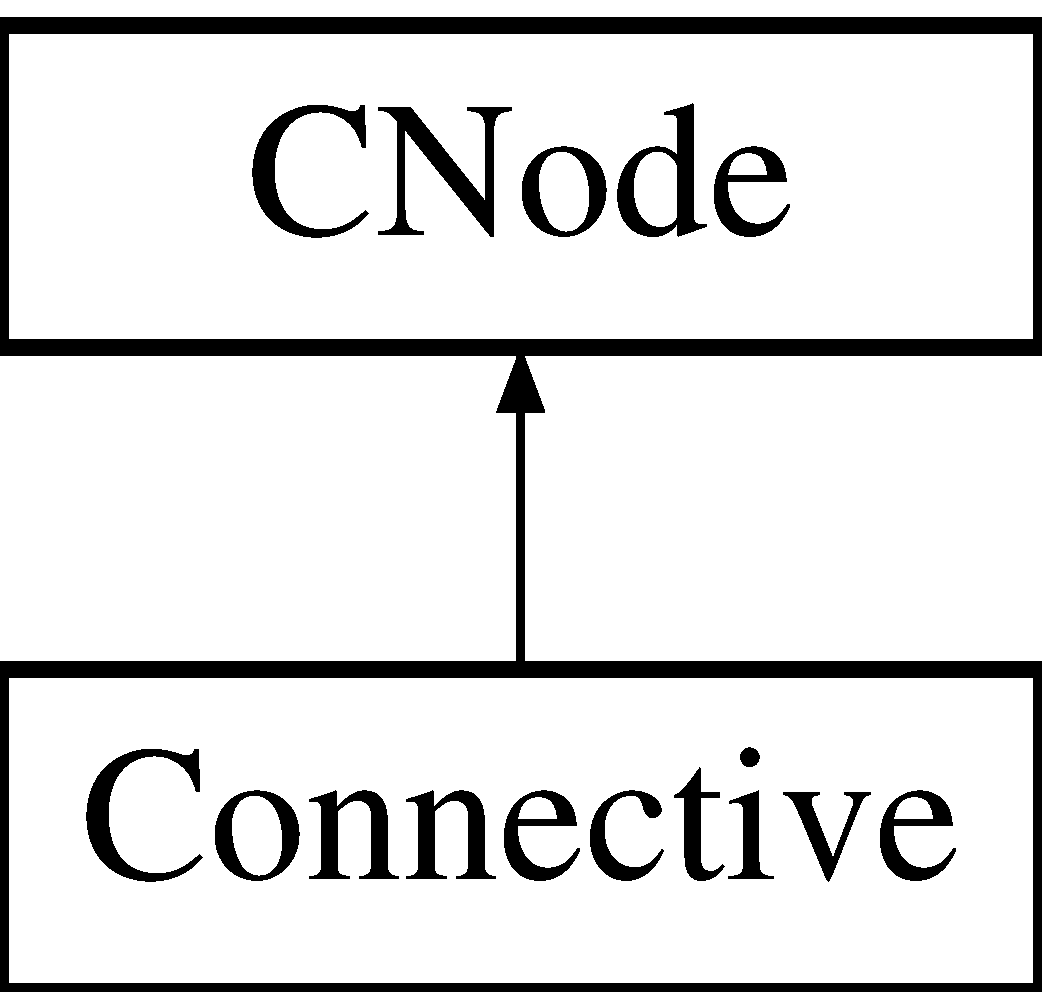
\includegraphics[height=2.000000cm]{classConnective}
\end{center}
\end{figure}
\subsection*{\-Public \-Member \-Functions}
\begin{DoxyCompactItemize}
\item 
\hypertarget{classConnective_a5fb6d4411e14493a4d8de27cc45bf616}{virtual bool {\bfseries operator==} (const \hyperlink{classCNode}{\-C\-Node} \&other)}\label{classConnective_a5fb6d4411e14493a4d8de27cc45bf616}

\item 
\hypertarget{classConnective_af8b03837853b2822a19cb9e500f3348b}{virtual string {\bfseries to\-\_\-string} ()}\label{classConnective_af8b03837853b2822a19cb9e500f3348b}

\item 
\hypertarget{classConnective_a735578c9ea3e025b1b11731e2adfc130}{const set$<$ \hyperlink{classCNode}{\-C\-Node} $\ast$ $>$ \& {\bfseries get\-\_\-operands} ()}\label{classConnective_a735578c9ea3e025b1b11731e2adfc130}

\item 
\hypertarget{classConnective_a0abec80116d43a285485d1a7e641766f}{virtual \hyperlink{classCNode}{\-C\-Node} $\ast$ {\bfseries substitute} (map$<$ \hyperlink{classTerm}{\-Term} $\ast$, \hyperlink{classTerm}{\-Term} $\ast$ $>$ \&subs)}\label{classConnective_a0abec80116d43a285485d1a7e641766f}

\end{DoxyCompactItemize}
\subsection*{\-Static \-Public \-Member \-Functions}
\begin{DoxyCompactItemize}
\item 
\hypertarget{classConnective_a9db2e5c1275ed1d7750ff42443642c5d}{static \hyperlink{classCNode}{\-C\-Node} $\ast$ {\bfseries make\-\_\-and} (const set$<$ \hyperlink{classCNode}{\-C\-Node} $\ast$ $>$ \&ops, bool simplify=true)}\label{classConnective_a9db2e5c1275ed1d7750ff42443642c5d}

\item 
\hypertarget{classConnective_a893b5c22ebdbc8f8729eccbf8044fff5}{static \hyperlink{classCNode}{\-C\-Node} $\ast$ {\bfseries make\-\_\-or} (const set$<$ \hyperlink{classCNode}{\-C\-Node} $\ast$ $>$ \&ops, bool simplify=true)}\label{classConnective_a893b5c22ebdbc8f8729eccbf8044fff5}

\item 
\hypertarget{classConnective_a2bfa7d0a5a2b483c951c2c141598544b}{static \hyperlink{classCNode}{\-C\-Node} $\ast$ {\bfseries make\-\_\-implies} (\hyperlink{classCNode}{\-C\-Node} $\ast$p, \hyperlink{classCNode}{\-C\-Node} $\ast$a)}\label{classConnective_a2bfa7d0a5a2b483c951c2c141598544b}

\item 
\hypertarget{classConnective_aa7a4c06828b2b006363505a6b467e5b0}{static \hyperlink{classCNode}{\-C\-Node} $\ast$ {\bfseries make\-\_\-not} (\hyperlink{classCNode}{\-C\-Node} $\ast$op)}\label{classConnective_aa7a4c06828b2b006363505a6b467e5b0}

\item 
\hypertarget{classConnective_a6d244aaf1e1f14cab26ea9d7d47d4995}{static \hyperlink{classCNode}{\-C\-Node} $\ast$ {\bfseries make} (cnode\-\_\-type connective\-\_\-type, const set$<$ \hyperlink{classCNode}{\-C\-Node} $\ast$ $>$ \&ops)}\label{classConnective_a6d244aaf1e1f14cab26ea9d7d47d4995}

\item 
\hypertarget{classConnective_a32888e60780cee951a359faef478c8d0}{static \hyperlink{classCNode}{\-C\-Node} $\ast$ {\bfseries make} (cnode\-\_\-type connective\-\_\-type, \hyperlink{classCNode}{\-C\-Node} $\ast$op1, \hyperlink{classCNode}{\-C\-Node} $\ast$op2)}\label{classConnective_a32888e60780cee951a359faef478c8d0}

\end{DoxyCompactItemize}
\subsection*{\-Friends}
\begin{DoxyCompactItemize}
\item 
\hypertarget{classConnective_a552ea17ad95fff16941105e4aefb0752}{class {\bfseries \-I\-L\-P\-Leaf}}\label{classConnective_a552ea17ad95fff16941105e4aefb0752}

\item 
\hypertarget{classConnective_a0657a422d4ddc5f4a0ff56931b7d2767}{class {\bfseries \-C\-Node}}\label{classConnective_a0657a422d4ddc5f4a0ff56931b7d2767}

\item 
\hypertarget{classConnective_ac98d07dd8f7b70e16ccb9a01abf56b9c}{class {\bfseries boost\-::serialization\-::access}}\label{classConnective_ac98d07dd8f7b70e16ccb9a01abf56b9c}

\end{DoxyCompactItemize}


\-The documentation for this class was generated from the following files\-:\begin{DoxyCompactItemize}
\item 
cnode/\-Connective.\-h\item 
cnode/\-Connective.\-cpp\end{DoxyCompactItemize}

\hypertarget{classConstantTerm}{\section{\-Constant\-Term \-Class \-Reference}
\label{classConstantTerm}\index{\-Constant\-Term@{\-Constant\-Term}}
}
\-Inheritance diagram for \-Constant\-Term\-:\begin{figure}[H]
\begin{center}
\leavevmode
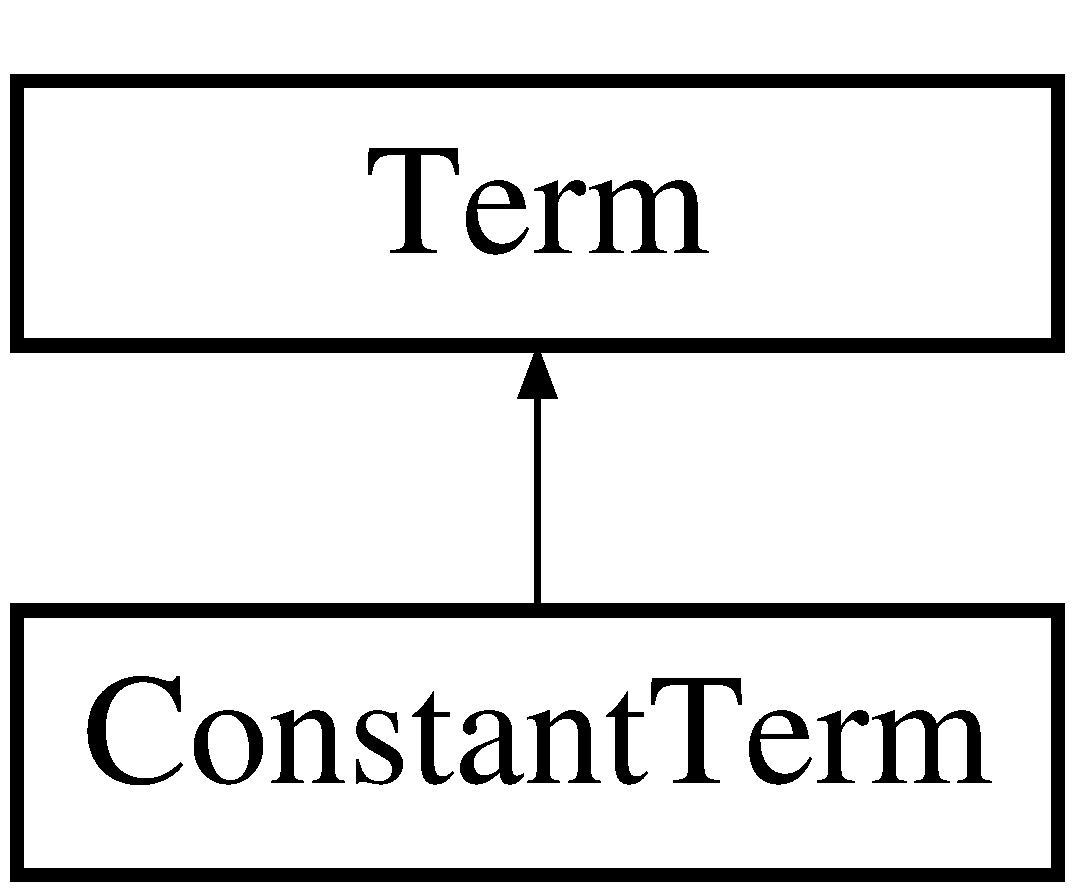
\includegraphics[height=2.000000cm]{classConstantTerm}
\end{center}
\end{figure}
\subsection*{\-Public \-Member \-Functions}
\begin{DoxyCompactItemize}
\item 
\hypertarget{classConstantTerm_abcdb55120fd16b9348a3a5b2f3a3c2fa}{{\bfseries \-Constant\-Term} (long int c)}\label{classConstantTerm_abcdb55120fd16b9348a3a5b2f3a3c2fa}

\item 
\hypertarget{classConstantTerm_ab7bd8a7f6ae006072ef51a2a9ec53bf0}{virtual bool {\bfseries operator==} (const \hyperlink{classTerm}{\-Term} \&other)}\label{classConstantTerm_ab7bd8a7f6ae006072ef51a2a9ec53bf0}

\item 
\hypertarget{classConstantTerm_ac720d945721c4d136a8bd8198fbf6f17}{virtual string {\bfseries to\-\_\-string} ()}\label{classConstantTerm_ac720d945721c4d136a8bd8198fbf6f17}

\item 
\hypertarget{classConstantTerm_a3fd40bae7e3822bf50fdd8f237a99bd7}{virtual \hyperlink{classTerm}{\-Term} $\ast$ {\bfseries substitute} (map$<$ \hyperlink{classTerm}{\-Term} $\ast$, \hyperlink{classTerm}{\-Term} $\ast$ $>$ \&subs)}\label{classConstantTerm_a3fd40bae7e3822bf50fdd8f237a99bd7}

\item 
\hypertarget{classConstantTerm_a541d6046999cccd83fdec132e09d2ee5}{long int {\bfseries get\-\_\-constant} ()}\label{classConstantTerm_a541d6046999cccd83fdec132e09d2ee5}

\end{DoxyCompactItemize}
\subsection*{\-Static \-Public \-Member \-Functions}
\begin{DoxyCompactItemize}
\item 
\hypertarget{classConstantTerm_a2b9c27b793e9dd5a2d97869dfab823cf}{static \hyperlink{classTerm}{\-Term} $\ast$ {\bfseries make} (long int c)}\label{classConstantTerm_a2b9c27b793e9dd5a2d97869dfab823cf}

\end{DoxyCompactItemize}
\subsection*{\-Friends}
\begin{DoxyCompactItemize}
\item 
\hypertarget{classConstantTerm_ac98d07dd8f7b70e16ccb9a01abf56b9c}{class {\bfseries boost\-::serialization\-::access}}\label{classConstantTerm_ac98d07dd8f7b70e16ccb9a01abf56b9c}

\end{DoxyCompactItemize}


\-The documentation for this class was generated from the following files\-:\begin{DoxyCompactItemize}
\item 
term/\-Constant\-Term.\-h\item 
term/\-Constant\-Term.\-cpp\end{DoxyCompactItemize}

\hypertarget{classConstraint}{\section{\-Constraint \-Class \-Reference}
\label{classConstraint}\index{\-Constraint@{\-Constraint}}
}
\subsection*{\-Public \-Member \-Functions}
\begin{DoxyCompactItemize}
\item 
\hyperlink{classConstraint_ae71d72d276e9659fabfc46fef811a028}{\-Constraint} (bool val)
\item 
\hypertarget{classConstraint_a00c534e4259ed3d1170bd4a4be0c791d}{{\bfseries \-Constraint} (const \hyperlink{classConstraint}{\-Constraint} \&nc, const \hyperlink{classConstraint}{\-Constraint} \&sc)}\label{classConstraint_a00c534e4259ed3d1170bd4a4be0c791d}

\item 
\hypertarget{classConstraint_a8a9db03093f7d3a866372091fbdb8ad1}{{\bfseries \-Constraint} (\hyperlink{classTerm}{\-Term} $\ast$t1, \hyperlink{classTerm}{\-Term} $\ast$t2, atom\-\_\-op\-\_\-type op)}\label{classConstraint_a8a9db03093f7d3a866372091fbdb8ad1}

\item 
\hypertarget{classConstraint_a425fef97454f148d33336ad5d2702efb}{{\bfseries \-Constraint} (const \hyperlink{classConstraint}{\-Constraint} \&other)}\label{classConstraint_a425fef97454f148d33336ad5d2702efb}

\item 
\hypertarget{classConstraint_a018537160b44de93f4cec08a5b98e566}{{\bfseries \-Constraint} (string s)}\label{classConstraint_a018537160b44de93f4cec08a5b98e566}

\item 
\hypertarget{classConstraint_a53f3ff0a5b48bc1d2ce09eff2bbeafd7}{{\bfseries \-Constraint} (const char $\ast$s)}\label{classConstraint_a53f3ff0a5b48bc1d2ce09eff2bbeafd7}

\item 
\hypertarget{classConstraint_a2add92afbe6070600d03e227c9707202}{{\bfseries \-Constraint} (\hyperlink{classCNode}{\-C\-Node} $\ast$n)}\label{classConstraint_a2add92afbe6070600d03e227c9707202}

\item 
\hypertarget{classConstraint_a11dec508c3495c846204417274363ea7}{bool {\bfseries sat} () const }\label{classConstraint_a11dec508c3495c846204417274363ea7}

\item 
\hypertarget{classConstraint_a9c5920cd6c466268623d02e6a8dec0a8}{bool {\bfseries unsat} () const }\label{classConstraint_a9c5920cd6c466268623d02e6a8dec0a8}

\item 
\hypertarget{classConstraint_a0aeb33d0859fe977b4ebe9a0c4388f80}{bool {\bfseries valid} () const }\label{classConstraint_a0aeb33d0859fe977b4ebe9a0c4388f80}

\item 
\hypertarget{classConstraint_a513104e3e2e3d937bf69bd31db952406}{bool {\bfseries equivalent} (\hyperlink{classConstraint}{\-Constraint} other) const }\label{classConstraint_a513104e3e2e3d937bf69bd31db952406}

\item 
\hypertarget{classConstraint_a16eef390b2a1174fee7302f8fa8ce47f}{bool {\bfseries sat\-\_\-discard} () const }\label{classConstraint_a16eef390b2a1174fee7302f8fa8ce47f}

\item 
\hypertarget{classConstraint_a9ec0c294cdf5617471b2f5dedcf576cc}{bool {\bfseries unsat\-\_\-discard} () const }\label{classConstraint_a9ec0c294cdf5617471b2f5dedcf576cc}

\item 
\hypertarget{classConstraint_abdfd75b78f0b60e837c9007c7384284d}{bool {\bfseries valid\-\_\-discard} () const }\label{classConstraint_abdfd75b78f0b60e837c9007c7384284d}

\item 
\hypertarget{classConstraint_a8cb788ba89071b63fb45c4101542b632}{\hyperlink{classConstraint}{\-Constraint} {\bfseries nc} () const }\label{classConstraint_a8cb788ba89071b63fb45c4101542b632}

\item 
\hypertarget{classConstraint_a341cc3ef346482fcb4e763662fd1c10c}{\hyperlink{classConstraint}{\-Constraint} {\bfseries sc} () const }\label{classConstraint_a341cc3ef346482fcb4e763662fd1c10c}

\item 
\hypertarget{classConstraint_a4c15a42e051b9d9f936e5c61f704cf6b}{int {\bfseries nc\-\_\-size} () const }\label{classConstraint_a4c15a42e051b9d9f936e5c61f704cf6b}

\item 
\hypertarget{classConstraint_a9cadd1975f3d26a4d58ce92362999a0b}{int {\bfseries sc\-\_\-size} () const }\label{classConstraint_a9cadd1975f3d26a4d58ce92362999a0b}

\item 
\hypertarget{classConstraint_ab4ea8f8060354f33b6a47757e919b6de}{bool {\bfseries is\-\_\-true} () const }\label{classConstraint_ab4ea8f8060354f33b6a47757e919b6de}

\item 
\hypertarget{classConstraint_adcd1a02849bd76c4aa40db13f24392a2}{bool {\bfseries is\-\_\-false} () const }\label{classConstraint_adcd1a02849bd76c4aa40db13f24392a2}

\item 
\hypertarget{classConstraint_a2a33670d51bf67ee84b788d51b68d4e5}{\hyperlink{classConstraint}{\-Constraint} {\bfseries operator\&} (const \hyperlink{classConstraint}{\-Constraint} \&other) const }\label{classConstraint_a2a33670d51bf67ee84b788d51b68d4e5}

\item 
\hypertarget{classConstraint_af5fc887697ec9958f0146c5c3d2dde3b}{\hyperlink{classConstraint}{\-Constraint} {\bfseries operator$|$} (const \hyperlink{classConstraint}{\-Constraint} \&other) const }\label{classConstraint_af5fc887697ec9958f0146c5c3d2dde3b}

\item 
\hypertarget{classConstraint_a7bb776021ac3f71c5d3fd2aaae573e50}{\hyperlink{classConstraint}{\-Constraint} {\bfseries abduce} (\hyperlink{classConstraint}{\-Constraint} b, const set$<$ \hyperlink{classConstraint}{\-Constraint} $>$ \&consistency\-\_\-constraints, map$<$ \hyperlink{classTerm}{\-Term} $\ast$, int $>$ \&costs) const }\label{classConstraint_a7bb776021ac3f71c5d3fd2aaae573e50}

\item 
\hypertarget{classConstraint_a0046df78524656d44014a637609867e5}{\hyperlink{classConstraint}{\-Constraint} {\bfseries abduce} (\hyperlink{classConstraint}{\-Constraint} b, const set$<$ \hyperlink{classConstraint}{\-Constraint} $>$ \&consistency\-\_\-constraints) const }\label{classConstraint_a0046df78524656d44014a637609867e5}

\item 
\hypertarget{classConstraint_a8e687501d399750ee3ede57853981128}{\hyperlink{classConstraint}{\-Constraint} {\bfseries abduce} (\hyperlink{classConstraint}{\-Constraint} b) const }\label{classConstraint_a8e687501d399750ee3ede57853981128}

\item 
\hypertarget{classConstraint_a31845ae694933cdb1df102b03ca15792}{void {\bfseries operator\&=} (const \hyperlink{classConstraint}{\-Constraint} \&other)}\label{classConstraint_a31845ae694933cdb1df102b03ca15792}

\item 
\hypertarget{classConstraint_abc1dedce9d25e37579700fd7a0756640}{void {\bfseries operator$|$=} (const \hyperlink{classConstraint}{\-Constraint} \&other)}\label{classConstraint_abc1dedce9d25e37579700fd7a0756640}

\item 
\hypertarget{classConstraint_a8f3d1d88c700cc778ab890d1a988beed}{\hyperlink{classConstraint}{\-Constraint} {\bfseries operator!} () const }\label{classConstraint_a8f3d1d88c700cc778ab890d1a988beed}

\item 
\hypertarget{classConstraint_a746cad20bfc4255820a3cc3333510f16}{void {\bfseries operator=} (const \hyperlink{classConstraint}{\-Constraint} \&other)}\label{classConstraint_a746cad20bfc4255820a3cc3333510f16}

\item 
\hypertarget{classConstraint_a8413aac9584a56afe3ab6d5038d3509a}{bool {\bfseries operator==} (const \hyperlink{classConstraint}{\-Constraint} \&other) const }\label{classConstraint_a8413aac9584a56afe3ab6d5038d3509a}

\item 
\hypertarget{classConstraint_a1d1067202e358f77ba72c4237b858f11}{bool {\bfseries operator!=} (const \hyperlink{classConstraint}{\-Constraint} \&other) const }\label{classConstraint_a1d1067202e358f77ba72c4237b858f11}

\item 
\hypertarget{classConstraint_ad74afe376931ccf0940c5cc60695536c}{bool {\bfseries implies} (const \hyperlink{classConstraint}{\-Constraint} \&other) const }\label{classConstraint_ad74afe376931ccf0940c5cc60695536c}

\item 
\hypertarget{classConstraint_a5836c0cfb47c3b6e61e2e99aa0893844}{bool {\bfseries operator$<$} (const \hyperlink{classConstraint}{\-Constraint} \&other) const }\label{classConstraint_a5836c0cfb47c3b6e61e2e99aa0893844}

\item 
\hypertarget{classConstraint_abe0d7e5f041e55fd5aacefbc1815b2a1}{bool {\bfseries is\-\_\-precise} () const }\label{classConstraint_abe0d7e5f041e55fd5aacefbc1815b2a1}

\item 
\hypertarget{classConstraint_a184cc1e313635131947554b72ae3faa9}{void {\bfseries eliminate\-\_\-evar} (\hyperlink{classVariableTerm}{\-Variable\-Term} $\ast$var)}\label{classConstraint_a184cc1e313635131947554b72ae3faa9}

\item 
\hypertarget{classConstraint_a2b3387858256afd188257eaa009da16d}{void {\bfseries eliminate\-\_\-evars} (set$<$ \hyperlink{classVariableTerm}{\-Variable\-Term} $\ast$ $>$ \&vars)}\label{classConstraint_a2b3387858256afd188257eaa009da16d}

\item 
\hypertarget{classConstraint_ac73c014f2e92c23f70392eb91d4c8565}{void {\bfseries eliminate\-\_\-uvar} (\hyperlink{classVariableTerm}{\-Variable\-Term} $\ast$var)}\label{classConstraint_ac73c014f2e92c23f70392eb91d4c8565}

\item 
\hypertarget{classConstraint_a12754a0a4ee272cea8fca8170f7cab5d}{void {\bfseries eliminate\-\_\-uvars} (set$<$ \hyperlink{classVariableTerm}{\-Variable\-Term} $\ast$ $>$ \&vars)}\label{classConstraint_a12754a0a4ee272cea8fca8170f7cab5d}

\item 
\hypertarget{classConstraint_ae8dfaa20ca8e1f4c464a40a9c11c3643}{bool {\bfseries contains\-\_\-inequality} ()}\label{classConstraint_ae8dfaa20ca8e1f4c464a40a9c11c3643}

\item 
\hypertarget{classConstraint_aa38c7080ec5d83c64c9093f4b81ec341}{void {\bfseries fresh\-\_\-id} ()}\label{classConstraint_aa38c7080ec5d83c64c9093f4b81ec341}

\item 
\hypertarget{classConstraint_a1b9f2421f5ac66f14524fdded2dfb762}{void {\bfseries eliminate\-\_\-free\-\_\-var} (\hyperlink{classVariableTerm}{\-Variable\-Term} $\ast$var)}\label{classConstraint_a1b9f2421f5ac66f14524fdded2dfb762}

\item 
\hypertarget{classConstraint_a5d4f06f6b68485a8e299e7b2d8b833b5}{void {\bfseries eliminate\-\_\-free\-\_\-vars} (set$<$ \hyperlink{classVariableTerm}{\-Variable\-Term} $\ast$ $>$ \&vars)}\label{classConstraint_a5d4f06f6b68485a8e299e7b2d8b833b5}

\item 
\hypertarget{classConstraint_a69517893aff23dee8ea80154467b2161}{void {\bfseries get\-\_\-terms} (set$<$ \hyperlink{classTerm}{\-Term} $\ast$ $>$ \&terms, bool include\-\_\-nested\-\_\-terms)}\label{classConstraint_a69517893aff23dee8ea80154467b2161}

\item 
\hypertarget{classConstraint_a06b67f3e9c44f5aab49007698fcd0b14}{\hyperlink{classTerm}{\-Term} $\ast$ {\bfseries find\-\_\-equality} (\hyperlink{classTerm}{\-Term} $\ast$t) const }\label{classConstraint_a06b67f3e9c44f5aab49007698fcd0b14}

\item 
\hypertarget{classConstraint_a5e2c9fc0f958461379dd08c0f55c7e51}{void {\bfseries find\-\_\-equalities} (\hyperlink{classTerm}{\-Term} $\ast$t, set$<$ \hyperlink{classTerm}{\-Term} $\ast$ $>$ \&eqs) const }\label{classConstraint_a5e2c9fc0f958461379dd08c0f55c7e51}

\item 
\hypertarget{classConstraint_a24eec2aa82235b851666c629df196f0a}{void {\bfseries replace\-\_\-term} (\hyperlink{classTerm}{\-Term} $\ast$to\-\_\-replace, \hyperlink{classTerm}{\-Term} $\ast$replacement)}\label{classConstraint_a24eec2aa82235b851666c629df196f0a}

\item 
\hypertarget{classConstraint_af9b206b82a008a4af7e1b575dc7d8ca7}{void {\bfseries replace\-\_\-terms} (map$<$ \hyperlink{classTerm}{\-Term} $\ast$, \hyperlink{classTerm}{\-Term} $\ast$ $>$ \&replacements)}\label{classConstraint_af9b206b82a008a4af7e1b575dc7d8ca7}

\item 
\hypertarget{classConstraint_a138adfd683910b897168e9e70fa10e42}{void {\bfseries replace\-\_\-constraint} (\hyperlink{classConstraint}{\-Constraint} to\-\_\-replace, \hyperlink{classConstraint}{\-Constraint} replacement)}\label{classConstraint_a138adfd683910b897168e9e70fa10e42}

\item 
\hypertarget{classConstraint_a81f4c55b35512008e41e3b5aeb1aa5e5}{void {\bfseries replace\-\_\-terms} (\hyperlink{classTerm}{\-Term} $\ast$($\ast$sub\-\_\-func)(\hyperlink{classTerm}{\-Term} $\ast$t, void $\ast$data), void $\ast$my\-\_\-data)}\label{classConstraint_a81f4c55b35512008e41e3b5aeb1aa5e5}

\item 
\hypertarget{classConstraint_ae1b1ebed8a9e9f7bee72831e047da334}{void {\bfseries get\-\_\-free\-\_\-variables} (set$<$ \hyperlink{classTerm}{\-Term} $\ast$ $>$ \&vars)}\label{classConstraint_ae1b1ebed8a9e9f7bee72831e047da334}

\item 
\hypertarget{classConstraint_a1d322a2774d5ec8b8c93c900dae0d984}{bool {\bfseries contains\-\_\-term} (\hyperlink{classTerm}{\-Term} $\ast$var)}\label{classConstraint_a1d322a2774d5ec8b8c93c900dae0d984}

\item 
\hypertarget{classConstraint_a2675221c52142359f0d76c9f84939352}{bool {\bfseries contains\-\_\-term} (set$<$ \hyperlink{classTerm}{\-Term} $\ast$ $>$ \&terms)}\label{classConstraint_a2675221c52142359f0d76c9f84939352}

\item 
\hypertarget{classConstraint_ae84415110bd11a02a9f1be31808e546d}{void {\bfseries propagate\-\_\-background} ()}\label{classConstraint_ae84415110bd11a02a9f1be31808e546d}

\item 
\hypertarget{classConstraint_a5b7687a87d44326b6b9e2cd63b4925f5}{void {\bfseries assume} (\hyperlink{classConstraint}{\-Constraint} c)}\label{classConstraint_a5b7687a87d44326b6b9e2cd63b4925f5}

\item 
\hypertarget{classConstraint_ae36861ed4c196be2d4e9824d6ba0c2d6}{bool {\bfseries has\-\_\-equality\-\_\-relation} (\hyperlink{classTerm}{\-Term} $\ast$t1, \hyperlink{classTerm}{\-Term} $\ast$t2)}\label{classConstraint_ae36861ed4c196be2d4e9824d6ba0c2d6}

\item 
\hypertarget{classConstraint_a7625a7c22ad175129c4fba0d67fb22b1}{void {\bfseries get\-\_\-disjunctive\-\_\-equalities} (\hyperlink{classTerm}{\-Term} $\ast$var, map$<$ \hyperlink{classTerm}{\-Term} $\ast$, \hyperlink{classConstraint}{\-Constraint} $>$ \&equalities)}\label{classConstraint_a7625a7c22ad175129c4fba0d67fb22b1}

\item 
\hypertarget{classConstraint_a0348a4d01b75f207d10b5ca8d526970f}{void {\bfseries divide} (long int c, \hyperlink{classTerm}{\-Term} $\ast$t)}\label{classConstraint_a0348a4d01b75f207d10b5ca8d526970f}

\item 
\hypertarget{classConstraint_aca5219e5b274f9ca2e0876b5cd41a45a}{bool {\bfseries get\-\_\-assignment} (set$<$ pair$<$ string, string $>$ $>$ \&assignments)}\label{classConstraint_aca5219e5b274f9ca2e0876b5cd41a45a}

\item 
\hypertarget{classConstraint_a714cc43955c92eaff09790db26bcce65}{bool {\bfseries get\-\_\-assignment} (map$<$ \hyperlink{classTerm}{\-Term} $\ast$, \hyperlink{classSatValue}{\-Sat\-Value} $>$ \&assignments)}\label{classConstraint_a714cc43955c92eaff09790db26bcce65}

\item 
\hypertarget{classConstraint_a02d6b2e562863ca2eae0d96a7b300dea}{void {\bfseries replace\-\_\-terms} (\hyperlink{classTerm}{\-Term} $\ast$($\ast$sub\-\_\-func)(\hyperlink{classTerm}{\-Term} $\ast$t))}\label{classConstraint_a02d6b2e562863ca2eae0d96a7b300dea}

\item 
\hypertarget{classConstraint_a947b983b8463eefe8d90f536211f4a10}{string {\bfseries to\-\_\-string} () const }\label{classConstraint_a947b983b8463eefe8d90f536211f4a10}

\item 
\hypertarget{classConstraint_a6f31b5e7a2f0df26f15ffd533753f8c8}{string {\bfseries debug\-\_\-string} ()}\label{classConstraint_a6f31b5e7a2f0df26f15ffd533753f8c8}

\item 
\hypertarget{classConstraint_a70a760c53060ed4d6b3810f92164d42c}{int {\bfseries msa} (map$<$ \hyperlink{classTerm}{\-Term} $\ast$, \hyperlink{classSatValue}{\-Sat\-Value} $>$ \&msa)}\label{classConstraint_a70a760c53060ed4d6b3810f92164d42c}

\item 
\hypertarget{classConstraint_aa22f7e399260fded2bb0c4601b6f56ca}{int {\bfseries msa} (set$<$ \hyperlink{classVariableTerm}{\-Variable\-Term} $\ast$ $>$ \&msa) const }\label{classConstraint_aa22f7e399260fded2bb0c4601b6f56ca}

\item 
\hypertarget{classConstraint_a5a399e2e9b5fb661a529eac2a9bb44fb}{int {\bfseries msa} (set$<$ \hyperlink{classVariableTerm}{\-Variable\-Term} $\ast$ $>$ \&msa, set$<$ \hyperlink{classConstraint}{\-Constraint} $>$ \&bg) const }\label{classConstraint_a5a399e2e9b5fb661a529eac2a9bb44fb}

\item 
\hypertarget{classConstraint_a7a2c968ae20470063ad0267349194df9}{int {\bfseries msa} (map$<$ \hyperlink{classTerm}{\-Term} $\ast$, \hyperlink{classSatValue}{\-Sat\-Value} $>$ \&msa, set$<$ \hyperlink{classConstraint}{\-Constraint} $>$ \&bg)}\label{classConstraint_a7a2c968ae20470063ad0267349194df9}

\item 
\hypertarget{classConstraint_a2479161a01c443f4eb224b7fb7217362}{int {\bfseries msa} (set$<$ \hyperlink{classVariableTerm}{\-Variable\-Term} $\ast$ $>$ \&msa, map$<$ \hyperlink{classVariableTerm}{\-Variable\-Term} $\ast$, int $>$ \&costs) const }\label{classConstraint_a2479161a01c443f4eb224b7fb7217362}

\item 
\hypertarget{classConstraint_a7c474fbddf288ae4d434ad522e3f77d2}{int {\bfseries msa} (set$<$ \hyperlink{classVariableTerm}{\-Variable\-Term} $\ast$ $>$ \&msa, set$<$ \hyperlink{classConstraint}{\-Constraint} $>$ \&bg, map$<$ \hyperlink{classVariableTerm}{\-Variable\-Term} $\ast$, int $>$ \&costs) const }\label{classConstraint_a7c474fbddf288ae4d434ad522e3f77d2}

\item 
\hypertarget{classConstraint_a59bc13545b1cba70b4f019510d0dab30}{int {\bfseries msa} (map$<$ \hyperlink{classTerm}{\-Term} $\ast$, \hyperlink{classSatValue}{\-Sat\-Value} $>$ \&msa, set$<$ \hyperlink{classConstraint}{\-Constraint} $>$ \&bg, map$<$ \hyperlink{classVariableTerm}{\-Variable\-Term} $\ast$, int $>$ \&costs)}\label{classConstraint_a59bc13545b1cba70b4f019510d0dab30}

\item 
\hypertarget{classConstraint_a7603703631bdfa99a92fc29ad23b59fd}{pair$<$ \hyperlink{classCNode}{\-C\-Node} $\ast$, \hyperlink{classCNode}{\-C\-Node} $\ast$ $>$ {\bfseries get\-\_\-cnodes} ()}\label{classConstraint_a7603703631bdfa99a92fc29ad23b59fd}

\item 
\hypertarget{classConstraint_a908183e353cf3c339b603a9c978cde39}{void {\bfseries to\-\_\-dnf} (set$<$ \hyperlink{classConstraint}{\-Constraint} $>$ \&dnf)}\label{classConstraint_a908183e353cf3c339b603a9c978cde39}

\item 
\hypertarget{classConstraint_aff927a53efaba215dda8c0a84ece19d0}{void {\bfseries to\-\_\-cnf} (set$<$ \hyperlink{classConstraint}{\-Constraint} $>$ \&cnf)}\label{classConstraint_aff927a53efaba215dda8c0a84ece19d0}

\end{DoxyCompactItemize}
\subsection*{\-Static \-Public \-Member \-Functions}
\begin{DoxyCompactItemize}
\item 
\hypertarget{classConstraint_ab8cca1b45048e8636c600447779d9a4e}{static void {\bfseries set\-\_\-geqz\-\_\-attribute} (\hyperlink{classTerm}{\-Term} $\ast$t)}\label{classConstraint_ab8cca1b45048e8636c600447779d9a4e}

\item 
\hypertarget{classConstraint_ac8e23416503e7bf0346b2edd9cbc1cd8}{static void {\bfseries set\-\_\-gtz\-\_\-attribute} (\hyperlink{classTerm}{\-Term} $\ast$t)}\label{classConstraint_ac8e23416503e7bf0346b2edd9cbc1cd8}

\item 
\hypertarget{classConstraint_a46d619dde16a00ac444ba79394a38ecd}{static void {\bfseries clear} ()}\label{classConstraint_a46d619dde16a00ac444ba79394a38ecd}

\item 
\hypertarget{classConstraint_a67937d78172d09bcaf40f23b7c710018}{static void {\bfseries add\-\_\-ground\-\_\-axiom} (\hyperlink{classConstraint}{\-Constraint} key, \hyperlink{classConstraint}{\-Constraint} c)}\label{classConstraint_a67937d78172d09bcaf40f23b7c710018}

\item 
\hypertarget{classConstraint_a307d00bfc95bf0daa524859beb86b564}{static void {\bfseries add\-\_\-quantified\-\_\-axiom} (\hyperlink{classConstraint}{\-Constraint} key, \hyperlink{classConstraint}{\-Constraint} c)}\label{classConstraint_a307d00bfc95bf0daa524859beb86b564}

\item 
\hypertarget{classConstraint_af7af81b8220a4c108232700174f04b82}{static void {\bfseries set\-\_\-background\-\_\-knowledge} (\hyperlink{classConstraint}{\-Constraint} c)}\label{classConstraint_af7af81b8220a4c108232700174f04b82}

\item 
\hypertarget{classConstraint_ab4098d783f79be9e34f7ba7e19eae1df}{static void {\bfseries replace\-\_\-term\-\_\-in\-\_\-axioms} (\hyperlink{classTerm}{\-Term} $\ast$old\-\_\-t, \hyperlink{classTerm}{\-Term} $\ast$new\-\_\-t)}\label{classConstraint_ab4098d783f79be9e34f7ba7e19eae1df}

\item 
\hypertarget{classConstraint_a2aab071fed7d175ba5a38df060f737bb}{static string {\bfseries background\-\_\-knowledge\-\_\-to\-\_\-string} ()}\label{classConstraint_a2aab071fed7d175ba5a38df060f737bb}

\item 
\hypertarget{classConstraint_a81da58b478cfc08940c997dddc7eed05}{static \hyperlink{classConstraint}{\-Constraint} {\bfseries get\-\_\-general\-\_\-background} ()}\label{classConstraint_a81da58b478cfc08940c997dddc7eed05}

\item 
\hypertarget{classConstraint_a40edd25142685c6b70b4ef1b829428b3}{static void {\bfseries clear\-\_\-background} ()}\label{classConstraint_a40edd25142685c6b70b4ef1b829428b3}

\item 
\hypertarget{classConstraint_a46b127b22500a32d9016a21a0c7c523c}{static void {\bfseries disable\-\_\-background} ()}\label{classConstraint_a46b127b22500a32d9016a21a0c7c523c}

\end{DoxyCompactItemize}
\subsection*{\-Static \-Public \-Attributes}
\begin{DoxyCompactItemize}
\item 
\hypertarget{classConstraint_ae55d1e2b3842e37c7125abf5d9fb03db}{static \hyperlink{classConstraintSolver}{\-Constraint\-Solver} {\bfseries cs}}\label{classConstraint_ae55d1e2b3842e37c7125abf5d9fb03db}

\end{DoxyCompactItemize}
\subsection*{\-Friends}
\begin{DoxyCompactItemize}
\item 
\hypertarget{classConstraint_ac98d07dd8f7b70e16ccb9a01abf56b9c}{class {\bfseries boost\-::serialization\-::access}}\label{classConstraint_ac98d07dd8f7b70e16ccb9a01abf56b9c}

\item 
\hypertarget{classConstraint_a5c4db00ea43b0e1ba711f807f6ddafc7}{struct {\bfseries std\-::hash$<$ Constraint $>$}}\label{classConstraint_a5c4db00ea43b0e1ba711f807f6ddafc7}

\item 
\hypertarget{classConstraint_a9604aeb393ba731519e459cdd02b09ff}{class {\bfseries \-Constraint\-Solver}}\label{classConstraint_a9604aeb393ba731519e459cdd02b09ff}

\item 
\hypertarget{classConstraint_a93def3190d5eacce69517079e5886ec2}{class {\bfseries \-Term}}\label{classConstraint_a93def3190d5eacce69517079e5886ec2}

\end{DoxyCompactItemize}


\subsection{\-Constructor \& \-Destructor \-Documentation}
\hypertarget{classConstraint_ae71d72d276e9659fabfc46fef811a028}{\index{\-Constraint@{\-Constraint}!\-Constraint@{\-Constraint}}
\index{\-Constraint@{\-Constraint}!Constraint@{\-Constraint}}
\subsubsection[{\-Constraint}]{\setlength{\rightskip}{0pt plus 5cm}\-Constraint\-::\-Constraint (
\begin{DoxyParamCaption}
\item[{bool}]{val}
\end{DoxyParamCaption}
)}}\label{classConstraint_ae71d72d276e9659fabfc46fef811a028}
\-Constructs boolean constant true/false 

\-The documentation for this class was generated from the following files\-:\begin{DoxyCompactItemize}
\item 
\-Constraint.\-h\item 
\-Constraint.\-cpp\end{DoxyCompactItemize}

\hypertarget{classConstraintSolver}{\section{\-Constraint\-Solver \-Class \-Reference}
\label{classConstraintSolver}\index{\-Constraint\-Solver@{\-Constraint\-Solver}}
}
\subsection*{\-Public \-Member \-Functions}
\begin{DoxyCompactItemize}
\item 
\hypertarget{classConstraintSolver_ad278d3c44ad966c1d816756350a49e2a}{void {\bfseries clear} ()}\label{classConstraintSolver_ad278d3c44ad966c1d816756350a49e2a}

\item 
\hypertarget{classConstraintSolver_abc3bd041971eb7c2a8c945fd345798bc}{void {\bfseries clear\-\_\-local\-\_\-data} ()}\label{classConstraintSolver_abc3bd041971eb7c2a8c945fd345798bc}

\item 
\hypertarget{classConstraintSolver_aba09ee6006bd332402370aa0273f29d8}{void {\bfseries clear\-\_\-stats} ()}\label{classConstraintSolver_aba09ee6006bd332402370aa0273f29d8}

\item 
\hypertarget{classConstraintSolver_a12fc56c78168495423040d1c3913fd7a}{string {\bfseries stats\-\_\-to\-\_\-string} ()}\label{classConstraintSolver_a12fc56c78168495423040d1c3913fd7a}

\end{DoxyCompactItemize}
\subsection*{\-Public \-Attributes}
\begin{DoxyCompactItemize}
\item 
\hypertarget{classConstraintSolver_a428f43f77725a42cb687e6b8f1a75659}{int {\bfseries num\-\_\-sat\-\_\-queries}}\label{classConstraintSolver_a428f43f77725a42cb687e6b8f1a75659}

\item 
\hypertarget{classConstraintSolver_a4a51de72ac1a6f7d9b4859a693e13b32}{int {\bfseries num\-\_\-bg\-\_\-queries}}\label{classConstraintSolver_a4a51de72ac1a6f7d9b4859a693e13b32}

\item 
\hypertarget{classConstraintSolver_a9f59908ea8c64a3c84a741fae2ef3863}{int {\bfseries solve\-\_\-time}}\label{classConstraintSolver_a9f59908ea8c64a3c84a741fae2ef3863}

\item 
\hypertarget{classConstraintSolver_afe5a1e9e69d4bcda19df66c174f227b8}{int {\bfseries eq\-\_\-time}}\label{classConstraintSolver_afe5a1e9e69d4bcda19df66c174f227b8}

\item 
\hypertarget{classConstraintSolver_a1b839e1c89ee06cf4ea4755c1d6dfa0c}{int {\bfseries num\-\_\-eqs}}\label{classConstraintSolver_a1b839e1c89ee06cf4ea4755c1d6dfa0c}

\item 
\hypertarget{classConstraintSolver_a65bc63411057c6e5aced8dbda0bcf537}{int {\bfseries bg\-\_\-simp\-\_\-time}}\label{classConstraintSolver_a65bc63411057c6e5aced8dbda0bcf537}

\item 
\hypertarget{classConstraintSolver_a217574336ec6ec9862e575e7d93aa660}{int {\bfseries num\-\_\-eliminate\-\_\-over\-\_\-queries}}\label{classConstraintSolver_a217574336ec6ec9862e575e7d93aa660}

\item 
\hypertarget{classConstraintSolver_a81d497f5e7c223161c22fe00015018b9}{int {\bfseries num\-\_\-eliminate\-\_\-under\-\_\-queries}}\label{classConstraintSolver_a81d497f5e7c223161c22fe00015018b9}

\item 
\hypertarget{classConstraintSolver_a78d9dd4dd6078ef21fa43d3f2b888d7e}{int {\bfseries eliminate\-\_\-over\-\_\-time}}\label{classConstraintSolver_a78d9dd4dd6078ef21fa43d3f2b888d7e}

\item 
\hypertarget{classConstraintSolver_a20ce49c30eab87d24b390a6aaa942971}{int {\bfseries eliminate\-\_\-under\-\_\-time}}\label{classConstraintSolver_a20ce49c30eab87d24b390a6aaa942971}

\end{DoxyCompactItemize}
\subsection*{\-Friends}
\begin{DoxyCompactItemize}
\item 
\hypertarget{classConstraintSolver_a697ed9eaa8955d595a023663ab1e8418}{class {\bfseries \-Constraint}}\label{classConstraintSolver_a697ed9eaa8955d595a023663ab1e8418}

\item 
\hypertarget{classConstraintSolver_a93def3190d5eacce69517079e5886ec2}{class {\bfseries \-Term}}\label{classConstraintSolver_a93def3190d5eacce69517079e5886ec2}

\end{DoxyCompactItemize}


\-The documentation for this class was generated from the following files\-:\begin{DoxyCompactItemize}
\item 
\-Constraint\-Solver.\-h\item 
\-Constraint\-Solver.\-cpp\end{DoxyCompactItemize}

\hypertarget{classCooper}{\section{\-Cooper \-Class \-Reference}
\label{classCooper}\index{\-Cooper@{\-Cooper}}
}
\subsection*{\-Public \-Member \-Functions}
\begin{DoxyCompactItemize}
\item 
\hypertarget{classCooper_a0c45eac5e0c933c60ca5c1a20983d9e1}{{\bfseries \-Cooper} (\hyperlink{classCNode}{\-C\-Node} $\ast$c, \hyperlink{classTerm}{\-Term} $\ast$elim\-\_\-t)}\label{classCooper_a0c45eac5e0c933c60ca5c1a20983d9e1}

\item 
\hypertarget{classCooper_acbfb11eb235246f921776450958bfa92}{\hyperlink{classCNode}{\-C\-Node} $\ast$ {\bfseries get\-\_\-result} ()}\label{classCooper_acbfb11eb235246f921776450958bfa92}

\end{DoxyCompactItemize}


\-The documentation for this class was generated from the following files\-:\begin{DoxyCompactItemize}
\item 
elimination/\-Cooper.\-h\item 
elimination/\-Cooper.\-cpp\end{DoxyCompactItemize}

\hypertarget{uniondata__type}{\section{data\-\_\-type \-Union \-Reference}
\label{uniondata__type}\index{data\-\_\-type@{data\-\_\-type}}
}
\subsection*{\-Public \-Attributes}
\begin{DoxyCompactItemize}
\item 
\hypertarget{uniondata__type_aca3953e2a01cbed3aacfbe4a4c1ac34e}{long int {\bfseries d}}\label{uniondata__type_aca3953e2a01cbed3aacfbe4a4c1ac34e}

\item 
\hypertarget{uniondata__type_abfeb2a93b035f875d6049f87f482c656}{mpz\-\_\-t {\bfseries i}}\label{uniondata__type_abfeb2a93b035f875d6049f87f482c656}

\end{DoxyCompactItemize}


\-The documentation for this union was generated from the following file\-:\begin{DoxyCompactItemize}
\item 
numeric-\/lib/bignum.\-h\end{DoxyCompactItemize}

\hypertarget{structDBClause}{\section{\-D\-B\-Clause \-Struct \-Reference}
\label{structDBClause}\index{\-D\-B\-Clause@{\-D\-B\-Clause}}
}
\subsection*{\-Public \-Member \-Functions}
\begin{DoxyCompactItemize}
\item 
\hypertarget{structDBClause_a83e0b7a5199569bb185463a536c80cbb}{{\bfseries \-D\-B\-Clause} (\hyperlink{classCNode}{\-C\-Node} $\ast$cl, set$<$ \hyperlink{classCNode}{\-C\-Node} $\ast$ $>$ \&l)}\label{structDBClause_a83e0b7a5199569bb185463a536c80cbb}

\end{DoxyCompactItemize}
\subsection*{\-Public \-Attributes}
\begin{DoxyCompactItemize}
\item 
\hypertarget{structDBClause_a2a5c384bc43691a6328110bfb5b7b98b}{\hyperlink{classCNode}{\-C\-Node} $\ast$ {\bfseries conflict\-\_\-clause}}\label{structDBClause_a2a5c384bc43691a6328110bfb5b7b98b}

\item 
\hypertarget{structDBClause_ac53163d7fd083c41b9eb7f89d5b256dc}{set$<$ \hyperlink{classCNode}{\-C\-Node} $\ast$ $>$ {\bfseries leaves}}\label{structDBClause_ac53163d7fd083c41b9eb7f89d5b256dc}

\end{DoxyCompactItemize}


\-The documentation for this struct was generated from the following files\-:\begin{DoxyCompactItemize}
\item 
solver/\-Conflict\-Database.\-h\item 
solver/\-Conflict\-Database.\-cpp\end{DoxyCompactItemize}

\hypertarget{structDBLeaf}{\section{\-D\-B\-Leaf \-Struct \-Reference}
\label{structDBLeaf}\index{\-D\-B\-Leaf@{\-D\-B\-Leaf}}
}
\subsection*{\-Public \-Member \-Functions}
\begin{DoxyCompactItemize}
\item 
\hypertarget{structDBLeaf_a714cc4ffefeadf3ff13b9ba448010a12}{{\bfseries \-D\-B\-Leaf} (\hyperlink{classLeaf}{\-Leaf} $\ast$l, \hyperlink{structDBClause}{\-D\-B\-Clause} $\ast$cl)}\label{structDBLeaf_a714cc4ffefeadf3ff13b9ba448010a12}

\end{DoxyCompactItemize}
\subsection*{\-Public \-Attributes}
\begin{DoxyCompactItemize}
\item 
\hypertarget{structDBLeaf_a5c755dbd54d03d5a0a835c61c2396342}{\hyperlink{classLeaf}{\-Leaf} $\ast$ {\bfseries l}}\label{structDBLeaf_a5c755dbd54d03d5a0a835c61c2396342}

\item 
\hypertarget{structDBLeaf_af8cc3f3efcb7cab4ddbade082ce81b21}{set$<$ \hyperlink{structDBClause}{\-D\-B\-Clause} $\ast$ $>$ {\bfseries conflict\-\_\-clauses}}\label{structDBLeaf_af8cc3f3efcb7cab4ddbade082ce81b21}

\end{DoxyCompactItemize}


\-The documentation for this struct was generated from the following files\-:\begin{DoxyCompactItemize}
\item 
solver/\-Conflict\-Database.\-h\item 
solver/\-Conflict\-Database.\-cpp\end{DoxyCompactItemize}

\hypertarget{structDeepEqual}{\section{\-Deep\-Equal$<$ \-K $>$ \-Struct \-Template \-Reference}
\label{structDeepEqual}\index{\-Deep\-Equal$<$ K $>$@{\-Deep\-Equal$<$ K $>$}}
}
\subsection*{\-Public \-Member \-Functions}
\begin{DoxyCompactItemize}
\item 
\hypertarget{structDeepEqual_ab33997826e0182fea574f49221e87342}{bool {\bfseries operator()} (const \-K $\ast$k1, const \-K $\ast$k2) const }\label{structDeepEqual_ab33997826e0182fea574f49221e87342}

\end{DoxyCompactItemize}
\subsubsection*{template$<$class K$>$ struct Deep\-Equal$<$ K $>$}



\-The documentation for this struct was generated from the following file\-:\begin{DoxyCompactItemize}
\item 
sat-\/solver/\-Map.\-h\end{DoxyCompactItemize}

\hypertarget{structDeepHash}{\section{\-Deep\-Hash$<$ \-K $>$ \-Struct \-Template \-Reference}
\label{structDeepHash}\index{\-Deep\-Hash$<$ K $>$@{\-Deep\-Hash$<$ K $>$}}
}
\subsection*{\-Public \-Member \-Functions}
\begin{DoxyCompactItemize}
\item 
\hypertarget{structDeepHash_a014f693e6a729f516fb1dfe4fd67d538}{uint32\-\_\-t {\bfseries operator()} (const \-K $\ast$k) const }\label{structDeepHash_a014f693e6a729f516fb1dfe4fd67d538}

\end{DoxyCompactItemize}
\subsubsection*{template$<$class K$>$ struct Deep\-Hash$<$ K $>$}



\-The documentation for this struct was generated from the following file\-:\begin{DoxyCompactItemize}
\item 
sat-\/solver/\-Map.\-h\end{DoxyCompactItemize}

\hypertarget{classDPLLSolver}{\section{\-D\-P\-L\-L\-Solver \-Class \-Reference}
\label{classDPLLSolver}\index{\-D\-P\-L\-L\-Solver@{\-D\-P\-L\-L\-Solver}}
}
\subsection*{\-Classes}
\begin{DoxyCompactItemize}
\item 
struct {\bfseries stack\-\_\-elem}
\end{DoxyCompactItemize}
\subsection*{\-Public \-Member \-Functions}
\begin{DoxyCompactItemize}
\item 
\hypertarget{classDPLLSolver_aaabd090084e867fb00c5ebb7ff82fef2}{{\bfseries \-D\-P\-L\-L\-Solver} (set$<$ \hyperlink{classTerm}{\-Term} $\ast$ $>$ \&ilp\-\_\-terms, map$<$ \hyperlink{classTerm}{\-Term} $\ast$, \hyperlink{classSatValue}{\-Sat\-Value} $>$ $\ast$assignments=\-N\-U\-L\-L)}\label{classDPLLSolver_aaabd090084e867fb00c5ebb7ff82fef2}

\item 
\hypertarget{classDPLLSolver_a610cf2273c5dc565c769c78cbf8c4901}{{\bfseries \-D\-P\-L\-L\-Solver} (\hyperlink{classCNode}{\-C\-Node} $\ast$theory\-\_\-tautologies, set$<$ \hyperlink{classTerm}{\-Term} $\ast$ $>$ \&ilp\-\_\-terms, map$<$ \hyperlink{classTerm}{\-Term} $\ast$, \hyperlink{classSatValue}{\-Sat\-Value} $>$ $\ast$assignments=\-N\-U\-L\-L)}\label{classDPLLSolver_a610cf2273c5dc565c769c78cbf8c4901}

\item 
\hypertarget{classDPLLSolver_ab6704d3098036e50cbc2cf6417d6a478}{void {\bfseries push} (\hyperlink{classCNode}{\-C\-Node} $\ast$c)}\label{classDPLLSolver_ab6704d3098036e50cbc2cf6417d6a478}

\item 
\hypertarget{classDPLLSolver_a8e30125c0474b450d5639dd4353b5828}{void {\bfseries pop} ()}\label{classDPLLSolver_a8e30125c0474b450d5639dd4353b5828}

\item 
\hypertarget{classDPLLSolver_a7da903735d63fb5a39160f1c564c7dfa}{\hyperlink{classCNode}{\-C\-Node} $\ast$ {\bfseries get\-\_\-stack} ()}\label{classDPLLSolver_a7da903735d63fb5a39160f1c564c7dfa}

\item 
\hypertarget{classDPLLSolver_a4c9e846203c9f0641a6aa88ffbe62d42}{void {\bfseries restrict} (\hyperlink{classCNode}{\-C\-Node} $\ast$background)}\label{classDPLLSolver_a4c9e846203c9f0641a6aa88ffbe62d42}

\item 
\hypertarget{classDPLLSolver_aa5b5907b0ca90447bd2fd57dc3a20b61}{bool {\bfseries is\-\_\-sat} ()}\label{classDPLLSolver_aa5b5907b0ca90447bd2fd57dc3a20b61}

\item 
\hypertarget{classDPLLSolver_ad631c1d00ab91fd8f62192cbd95ba21c}{\hyperlink{classCNode}{\-C\-Node} $\ast$ {\bfseries get\-\_\-background\-\_\-assumptions} ()}\label{classDPLLSolver_ad631c1d00ab91fd8f62192cbd95ba21c}

\item 
\hypertarget{classDPLLSolver_ab508b0a082d20e89ab49a0cdaa2479b6}{string {\bfseries get\-\_\-stats} ()}\label{classDPLLSolver_ab508b0a082d20e89ab49a0cdaa2479b6}

\item 
\hypertarget{classDPLLSolver_a3879075c66f882bd03d5950a39f8fa95}{\hyperlink{classCNode}{\-C\-Node} $\ast$ {\bfseries get\-\_\-current\-\_\-assignment} ()}\label{classDPLLSolver_a3879075c66f882bd03d5950a39f8fa95}

\item 
\hypertarget{classDPLLSolver_a506016ab888db5b911db88de4ba88fc2}{int {\bfseries get\-\_\-num\-\_\-consecutive\-\_\-boolean\-\_\-complete} () const }\label{classDPLLSolver_a506016ab888db5b911db88de4ba88fc2}

\item 
\hypertarget{classDPLLSolver_a9fcdffbba56b43867aa7c0df93b08bac}{double {\bfseries boolean\-\_\-complete\-\_\-ratio} () const }\label{classDPLLSolver_a9fcdffbba56b43867aa7c0df93b08bac}

\item 
\hypertarget{classDPLLSolver_aa1dcbd6358c3ceddff66a1c90e8bfed8}{double {\bfseries time\-\_\-verifying\-\_\-boolean\-\_\-assignment} () const }\label{classDPLLSolver_aa1dcbd6358c3ceddff66a1c90e8bfed8}

\item 
\hypertarget{classDPLLSolver_a0fd2424e651b2b8679f8ce4e12dd38f3}{int {\bfseries num\-\_\-clauses\-\_\-checked\-\_\-in\-\_\-theory} () const }\label{classDPLLSolver_a0fd2424e651b2b8679f8ce4e12dd38f3}

\item 
\hypertarget{classDPLLSolver_a54a36e043d82076fc80834e3fbeb470a}{\hyperlink{classCNode}{\-C\-Node} $\ast$ {\bfseries substitute\-\_\-partial\-\_\-assignment} (\hyperlink{classCNode}{\-C\-Node} $\ast$constraint)}\label{classDPLLSolver_a54a36e043d82076fc80834e3fbeb470a}

\end{DoxyCompactItemize}


\-The documentation for this class was generated from the following files\-:\begin{DoxyCompactItemize}
\item 
solver/\-D\-P\-L\-L\-Solver.\-h\item 
solver/\-D\-P\-L\-L\-Solver.\-cpp\end{DoxyCompactItemize}

\hypertarget{structeliminate__regression}{\section{eliminate\-\_\-regression \-Struct \-Reference}
\label{structeliminate__regression}\index{eliminate\-\_\-regression@{eliminate\-\_\-regression}}
}
\subsection*{\-Public \-Attributes}
\begin{DoxyCompactItemize}
\item 
\hypertarget{structeliminate__regression_a1157d737ce7deb0e2a58f303e658c51f}{string {\bfseries constraint}}\label{structeliminate__regression_a1157d737ce7deb0e2a58f303e658c51f}

\item 
\hypertarget{structeliminate__regression_a8e89e50d42be886e8525d2d9a468f350}{string {\bfseries elimination\-\_\-result}}\label{structeliminate__regression_a8e89e50d42be886e8525d2d9a468f350}

\end{DoxyCompactItemize}


\-The documentation for this struct was generated from the following file\-:\begin{DoxyCompactItemize}
\item 
ui/src/solver-\/ui.\-cpp\end{DoxyCompactItemize}

\hypertarget{classEqLeaf}{\section{\-Eq\-Leaf \-Class \-Reference}
\label{classEqLeaf}\index{\-Eq\-Leaf@{\-Eq\-Leaf}}
}
\-Inheritance diagram for \-Eq\-Leaf\-:\begin{figure}[H]
\begin{center}
\leavevmode
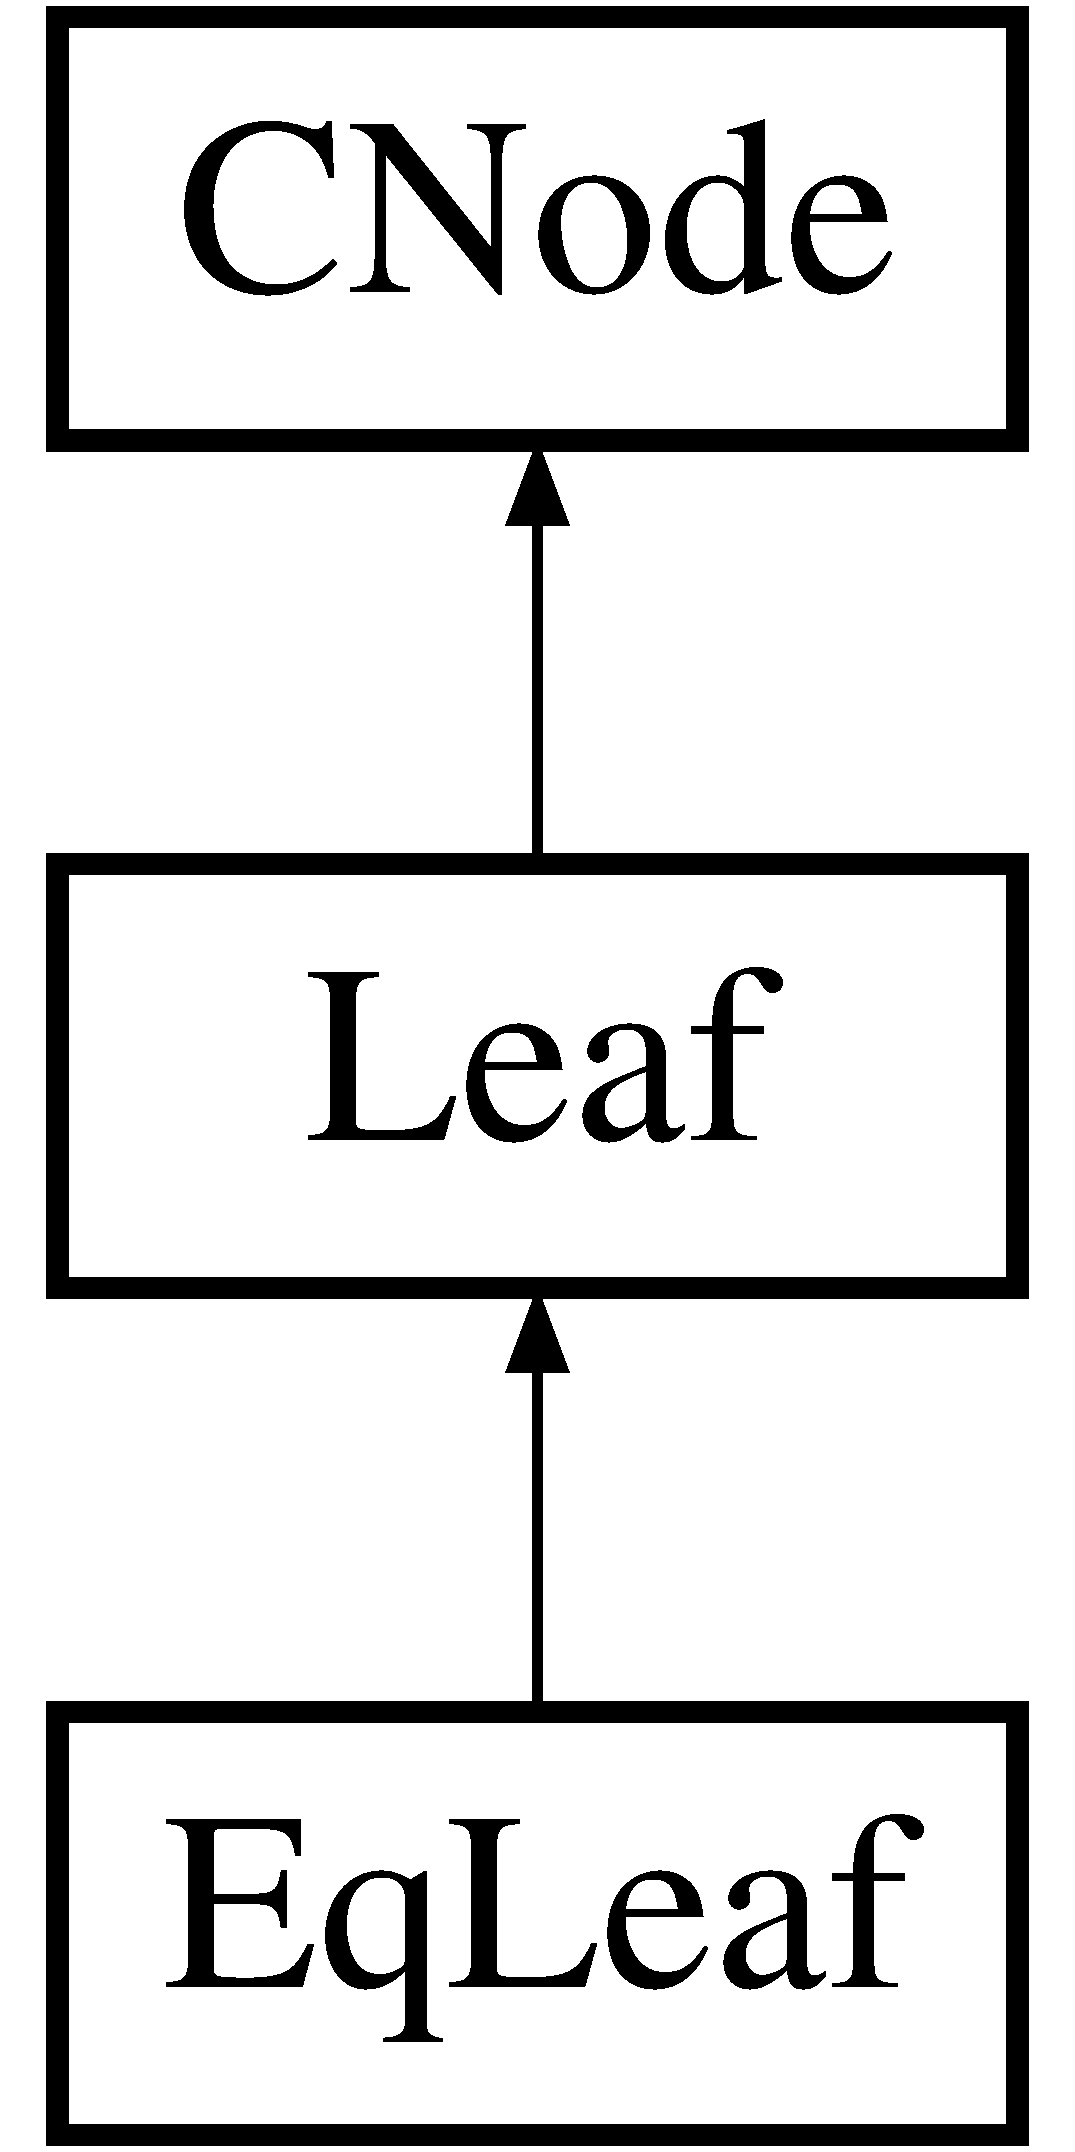
\includegraphics[height=3.000000cm]{classEqLeaf}
\end{center}
\end{figure}
\subsection*{\-Public \-Member \-Functions}
\begin{DoxyCompactItemize}
\item 
\hypertarget{classEqLeaf_ac6ce85eb42b25ad4874a5c8cdff44eda}{virtual bool {\bfseries operator==} (const \hyperlink{classCNode}{\-C\-Node} \&other)}\label{classEqLeaf_ac6ce85eb42b25ad4874a5c8cdff44eda}

\item 
\hypertarget{classEqLeaf_a4b3969b54279bbb77c932f7fdbf041b7}{virtual string {\bfseries to\-\_\-string} ()}\label{classEqLeaf_a4b3969b54279bbb77c932f7fdbf041b7}

\item 
\hypertarget{classEqLeaf_afed0df330cd40f9d00e8a7b77d7b6bef}{virtual \hyperlink{classCNode}{\-C\-Node} $\ast$ {\bfseries substitute} (map$<$ \hyperlink{classTerm}{\-Term} $\ast$, \hyperlink{classTerm}{\-Term} $\ast$ $>$ \&subs)}\label{classEqLeaf_afed0df330cd40f9d00e8a7b77d7b6bef}

\item 
\hypertarget{classEqLeaf_a3d070fd46c23c3da1195af86a142bf6d}{\hyperlink{classTerm}{\-Term} $\ast$ {\bfseries get\-\_\-lhs} ()}\label{classEqLeaf_a3d070fd46c23c3da1195af86a142bf6d}

\item 
\hypertarget{classEqLeaf_a234fdc257563c6ad10f1a9578b39191e}{\hyperlink{classTerm}{\-Term} $\ast$ {\bfseries get\-\_\-rhs} ()}\label{classEqLeaf_a234fdc257563c6ad10f1a9578b39191e}

\end{DoxyCompactItemize}
\subsection*{\-Static \-Public \-Member \-Functions}
\begin{DoxyCompactItemize}
\item 
\hypertarget{classEqLeaf_a23f7147fcee3e80acef2e09e4f7096d0}{static \hyperlink{classCNode}{\-C\-Node} $\ast$ {\bfseries make} (\hyperlink{classTerm}{\-Term} $\ast$lhs, \hyperlink{classTerm}{\-Term} $\ast$rhs)}\label{classEqLeaf_a23f7147fcee3e80acef2e09e4f7096d0}

\end{DoxyCompactItemize}
\subsection*{\-Protected \-Member \-Functions}
\begin{DoxyCompactItemize}
\item 
\hypertarget{classEqLeaf_a2b43d9474fd748cb3254aca661b69e68}{{\bfseries \-Eq\-Leaf} (\hyperlink{classTerm}{\-Term} $\ast$lhs, \hyperlink{classTerm}{\-Term} $\ast$rhs)}\label{classEqLeaf_a2b43d9474fd748cb3254aca661b69e68}

\end{DoxyCompactItemize}
\subsection*{\-Friends}
\begin{DoxyCompactItemize}
\item 
\hypertarget{classEqLeaf_ac98d07dd8f7b70e16ccb9a01abf56b9c}{class {\bfseries boost\-::serialization\-::access}}\label{classEqLeaf_ac98d07dd8f7b70e16ccb9a01abf56b9c}

\end{DoxyCompactItemize}


\-The documentation for this class was generated from the following files\-:\begin{DoxyCompactItemize}
\item 
cnode/\-Eq\-Leaf.\-h\item 
cnode/\-Eq\-Leaf.\-cpp\end{DoxyCompactItemize}

\hypertarget{structEqual}{\section{\-Equal$<$ \-K $>$ \-Struct \-Template \-Reference}
\label{structEqual}\index{\-Equal$<$ K $>$@{\-Equal$<$ K $>$}}
}
\subsection*{\-Public \-Member \-Functions}
\begin{DoxyCompactItemize}
\item 
\hypertarget{structEqual_aa134c69e7d7d04ac58043ed7f127e8d5}{bool {\bfseries operator()} (const \-K \&k1, const \-K \&k2) const }\label{structEqual_aa134c69e7d7d04ac58043ed7f127e8d5}

\end{DoxyCompactItemize}
\subsubsection*{template$<$class K$>$ struct Equal$<$ K $>$}



\-The documentation for this struct was generated from the following file\-:\begin{DoxyCompactItemize}
\item 
sat-\/solver/\-Map.\-h\end{DoxyCompactItemize}

\hypertarget{classEqualityFinder}{\section{\-Equality\-Finder \-Class \-Reference}
\label{classEqualityFinder}\index{\-Equality\-Finder@{\-Equality\-Finder}}
}
\subsection*{\-Public \-Member \-Functions}
\begin{DoxyCompactItemize}
\item 
\hypertarget{classEqualityFinder_a89494aed5b36818e300f60a280eb7496}{{\bfseries \-Equality\-Finder} (\hyperlink{classCNode}{\-C\-Node} $\ast$node, \hyperlink{classTerm}{\-Term} $\ast$var, bool find\-\_\-disjunctive\-\_\-eqs)}\label{classEqualityFinder_a89494aed5b36818e300f60a280eb7496}

\item 
\hypertarget{classEqualityFinder_a86ada1a0ee04376c9bc778025bc678d5}{const set$<$ \hyperlink{classTerm}{\-Term} $\ast$ $>$ \& {\bfseries get\-\_\-equalities} ()}\label{classEqualityFinder_a86ada1a0ee04376c9bc778025bc678d5}

\item 
\hypertarget{classEqualityFinder_a7f9323eda39ba6fecc3d1ca68d296361}{const map$<$ \hyperlink{classTerm}{\-Term} $\ast$, \hyperlink{classCNode}{\-C\-Node} $\ast$ $>$ \& {\bfseries get\-\_\-disjunctive\-\_\-equalities} ()}\label{classEqualityFinder_a7f9323eda39ba6fecc3d1ca68d296361}

\end{DoxyCompactItemize}


\-The documentation for this class was generated from the following files\-:\begin{DoxyCompactItemize}
\item 
solver/\-Equality\-Finder.\-h\item 
solver/\-Equality\-Finder.\-cpp\end{DoxyCompactItemize}

\hypertarget{classEquation}{\section{\-Equation \-Class \-Reference}
\label{classEquation}\index{\-Equation@{\-Equation}}
}
\subsection*{\-Public \-Member \-Functions}
\begin{DoxyCompactItemize}
\item 
\hypertarget{classEquation_a3d0b2d300421779d32991da6e75d8923}{{\bfseries \-Equation} (int cols, bool infinite)}\label{classEquation_a3d0b2d300421779d32991da6e75d8923}

\item 
\hypertarget{classEquation_a80df9d307bebd60b8df5aad3cde9b562}{void {\bfseries set\-\_\-initial\-\_\-value} (int c, \hyperlink{uniondata__type}{data\-\_\-type} d)}\label{classEquation_a80df9d307bebd60b8df5aad3cde9b562}

\item 
\hypertarget{classEquation_a5e1015cd498c3b66de2d0894f393f249}{size\-\_\-t {\bfseries compute\-\_\-hash\-\_\-d} ()}\label{classEquation_a5e1015cd498c3b66de2d0894f393f249}

\item 
\hypertarget{classEquation_a7001f49bc5c4988e6917c294589f8aa9}{size\-\_\-t {\bfseries compute\-\_\-hash\-\_\-i} ()}\label{classEquation_a7001f49bc5c4988e6917c294589f8aa9}

\item 
\hypertarget{classEquation_ad7116a9282cb349f9beb0b682a1b68bc}{void {\bfseries make\-\_\-infinite} ()}\label{classEquation_ad7116a9282cb349f9beb0b682a1b68bc}

\item 
\hypertarget{classEquation_a3c6502c0573d81abb203cf8856eb1dc1}{\hyperlink{classEquation}{\-Equation} $\ast$ {\bfseries clone} ()}\label{classEquation_a3c6502c0573d81abb203cf8856eb1dc1}

\item 
\hypertarget{classEquation_a582353148cbaaed08a132931033bab96}{void {\bfseries divide} (\hyperlink{classbignum}{bignum} b)}\label{classEquation_a582353148cbaaed08a132931033bab96}

\item 
\hypertarget{classEquation_a2ffaac9efb0d0f1190201a5da1625d23}{{\bfseries \-Equation} (int cols)}\label{classEquation_a2ffaac9efb0d0f1190201a5da1625d23}

\item 
\hypertarget{classEquation_a89987ec22fd6d12148217149076b42bc}{void {\bfseries set\-\_\-proof} ()}\label{classEquation_a89987ec22fd6d12148217149076b42bc}

\item 
\hypertarget{classEquation_af9da212e3e0d5da196c7ae3c981ee925}{void {\bfseries unset\-\_\-proof} ()}\label{classEquation_af9da212e3e0d5da196c7ae3c981ee925}

\item 
\hypertarget{classEquation_a8d8fd4ab3a72786ffbc0bf07153362ca}{bool {\bfseries is\-\_\-proof} ()}\label{classEquation_a8d8fd4ab3a72786ffbc0bf07153362ca}

\item 
\hypertarget{classEquation_a6fce9da19cf98288f3150279bd4c8e17}{\hyperlink{classbignum}{bignum} {\bfseries compute\-\_\-gcd} (bool skip\-\_\-last=false)}\label{classEquation_a6fce9da19cf98288f3150279bd4c8e17}

\item 
\hypertarget{classEquation_aa2b2811df7e0996d5432b30952a4ea79}{int {\bfseries get\-\_\-cols} ()}\label{classEquation_aa2b2811df7e0996d5432b30952a4ea79}

\item 
\hypertarget{classEquation_a3df4ed00b73ec516c53c86f379bf9c9c}{bool {\bfseries satisfies} (vector$<$ \hyperlink{classbigfraction}{bigfraction} $>$ \&a)}\label{classEquation_a3df4ed00b73ec516c53c86f379bf9c9c}

\item 
\hypertarget{classEquation_ae40ffbd2ba1d58b21b0d633ff593b422}{\hyperlink{classbigfraction}{bigfraction} {\bfseries evaluate} (vector$<$ \hyperlink{classbigfraction}{bigfraction} $>$ \&a)}\label{classEquation_ae40ffbd2ba1d58b21b0d633ff593b422}

\item 
\hypertarget{classEquation_a8a01e94de09a9e9ad0afe02b68780090}{void {\bfseries set} (int c, const \hyperlink{classbignum}{bignum} b)}\label{classEquation_a8a01e94de09a9e9ad0afe02b68780090}

\item 
\hypertarget{classEquation_a2ccd7f85ee2504faf9aa99b103c91ab8}{void {\bfseries flip\-\_\-sign} ()}\label{classEquation_a2ccd7f85ee2504faf9aa99b103c91ab8}

\item 
\hypertarget{classEquation_abda0dfa8da838efdf6ebb688d9181b58}{void {\bfseries flip\-\_\-sign} (int c)}\label{classEquation_abda0dfa8da838efdf6ebb688d9181b58}

\item 
\hypertarget{classEquation_a1e06388082f2d0053d59a1b002031359}{\hyperlink{classbignum}{bignum} {\bfseries get} (int c)}\label{classEquation_a1e06388082f2d0053d59a1b002031359}

\item 
\hypertarget{classEquation_a3f462be768a1a3de41082a105b136df5}{size\-\_\-t {\bfseries hash\-\_\-code} ()}\label{classEquation_a3f462be768a1a3de41082a105b136df5}

\item 
\hypertarget{classEquation_a56e0c6c802852672d550d7b3a3b2c7e1}{int {\bfseries num\-\_\-entries} ()}\label{classEquation_a56e0c6c802852672d550d7b3a3b2c7e1}

\item 
\hypertarget{classEquation_a4eb002a82db6629cc7c03e2aa7edbcd7}{string {\bfseries to\-\_\-string} ()}\label{classEquation_a4eb002a82db6629cc7c03e2aa7edbcd7}

\item 
\hypertarget{classEquation_afc920060931a12dd17d3eba1d5b841eb}{bool {\bfseries operator==} (\hyperlink{classEquation}{\-Equation} \&other)}\label{classEquation_afc920060931a12dd17d3eba1d5b841eb}

\item 
\hypertarget{classEquation_a63a03eff507ce27ce0e7847d5b64f2a0}{bool {\bfseries operator$<$} (\hyperlink{classEquation}{\-Equation} \&other)}\label{classEquation_a63a03eff507ce27ce0e7847d5b64f2a0}

\item 
\hypertarget{classEquation_aceed96723d9171e3ae90556d3f95d34d}{bool {\bfseries operator!=} (\hyperlink{classEquation}{\-Equation} \&other)}\label{classEquation_aceed96723d9171e3ae90556d3f95d34d}

\end{DoxyCompactItemize}
\subsection*{\-Public \-Attributes}
\begin{DoxyCompactItemize}
\item 
\hypertarget{classEquation_aff1a32ea7d7e1939439961668b604507}{\hyperlink{uniondata__type}{data\-\_\-type} $\ast$ {\bfseries eq}}\label{classEquation_aff1a32ea7d7e1939439961668b604507}

\item 
\hypertarget{classEquation_a46d28bf480c4f9f4d21e9f5c6c9e1ae5}{int {\bfseries cols}}\label{classEquation_a46d28bf480c4f9f4d21e9f5c6c9e1ae5}

\item 
\hypertarget{classEquation_a0dd3722641518121376463311d152fb2}{bool {\bfseries infinite}}\label{classEquation_a0dd3722641518121376463311d152fb2}

\item 
\hypertarget{classEquation_a7313041c526f4b27fead1c8474d72ba1}{bool {\bfseries proof}}\label{classEquation_a7313041c526f4b27fead1c8474d72ba1}

\end{DoxyCompactItemize}
\subsection*{\-Friends}
\begin{DoxyCompactItemize}
\item 
\hypertarget{classEquation_a719939672fd1aff22cf454d1d3468b00}{class {\bfseries slack\-\_\-matrix}}\label{classEquation_a719939672fd1aff22cf454d1d3468b00}

\item 
\hypertarget{classEquation_a948d3097bdf1b96c0bf30cf8abd5600e}{ostream \& {\bfseries operator$<$$<$} (ostream \&os, const \hyperlink{classEquation}{\-Equation} \&obj)}\label{classEquation_a948d3097bdf1b96c0bf30cf8abd5600e}

\end{DoxyCompactItemize}


\-The documentation for this class was generated from the following file\-:\begin{DoxyCompactItemize}
\item 
solver/\-Equation.\-h\end{DoxyCompactItemize}

\hypertarget{structequation__eq}{\section{equation\-\_\-eq \-Struct \-Reference}
\label{structequation__eq}\index{equation\-\_\-eq@{equation\-\_\-eq}}
}
\subsection*{\-Public \-Member \-Functions}
\begin{DoxyCompactItemize}
\item 
\hypertarget{structequation__eq_a12efd07dfa14fef54d83b88d85766d3a}{bool {\bfseries operator()} (const \hyperlink{classEquation}{\-Equation} $\ast$const \-\_\-e1, const \hyperlink{classEquation}{\-Equation} $\ast$const \-\_\-e2) const }\label{structequation__eq_a12efd07dfa14fef54d83b88d85766d3a}

\end{DoxyCompactItemize}


\-The documentation for this struct was generated from the following file\-:\begin{DoxyCompactItemize}
\item 
solver/\-Equation.\-h\end{DoxyCompactItemize}

\hypertarget{structequation__lt}{\section{equation\-\_\-lt \-Struct \-Reference}
\label{structequation__lt}\index{equation\-\_\-lt@{equation\-\_\-lt}}
}
\subsection*{\-Public \-Member \-Functions}
\begin{DoxyCompactItemize}
\item 
\hypertarget{structequation__lt_afa9c6862b5e09c5e15126715362c08df}{bool {\bfseries operator()} (const \hyperlink{classEquation}{\-Equation} $\ast$const \-\_\-e1, const \hyperlink{classEquation}{\-Equation} $\ast$const \-\_\-e2) const }\label{structequation__lt_afa9c6862b5e09c5e15126715362c08df}

\end{DoxyCompactItemize}


\-The documentation for this struct was generated from the following file\-:\begin{DoxyCompactItemize}
\item 
solver/\-Equation.\-h\end{DoxyCompactItemize}

\hypertarget{classExistentialEliminator}{\section{\-Existential\-Eliminator \-Class \-Reference}
\label{classExistentialEliminator}\index{\-Existential\-Eliminator@{\-Existential\-Eliminator}}
}
\subsection*{\-Public \-Member \-Functions}
\begin{DoxyCompactItemize}
\item 
\hypertarget{classExistentialEliminator_a67bb7978f5b99a559a5f61cf60be1fbd}{{\bfseries \-Existential\-Eliminator} (\hyperlink{classCNode}{\-C\-Node} $\ast$c, \hyperlink{classTerm}{\-Term} $\ast$t, bool overapproximation)}\label{classExistentialEliminator_a67bb7978f5b99a559a5f61cf60be1fbd}

\item 
\hypertarget{classExistentialEliminator_ae14a3917156d8feb30319a3da0f7be46}{\hyperlink{classCNode}{\-C\-Node} $\ast$ {\bfseries get\-\_\-result} ()}\label{classExistentialEliminator_ae14a3917156d8feb30319a3da0f7be46}

\end{DoxyCompactItemize}


\-The documentation for this class was generated from the following files\-:\begin{DoxyCompactItemize}
\item 
elimination/\-Existential\-Eliminator.\-h\item 
elimination/\-Existential\-Eliminator.\-cpp\end{DoxyCompactItemize}

\hypertarget{classFalse}{\section{\-False \-Class \-Reference}
\label{classFalse}\index{\-False@{\-False}}
}
\-Inheritance diagram for \-False\-:\begin{figure}[H]
\begin{center}
\leavevmode
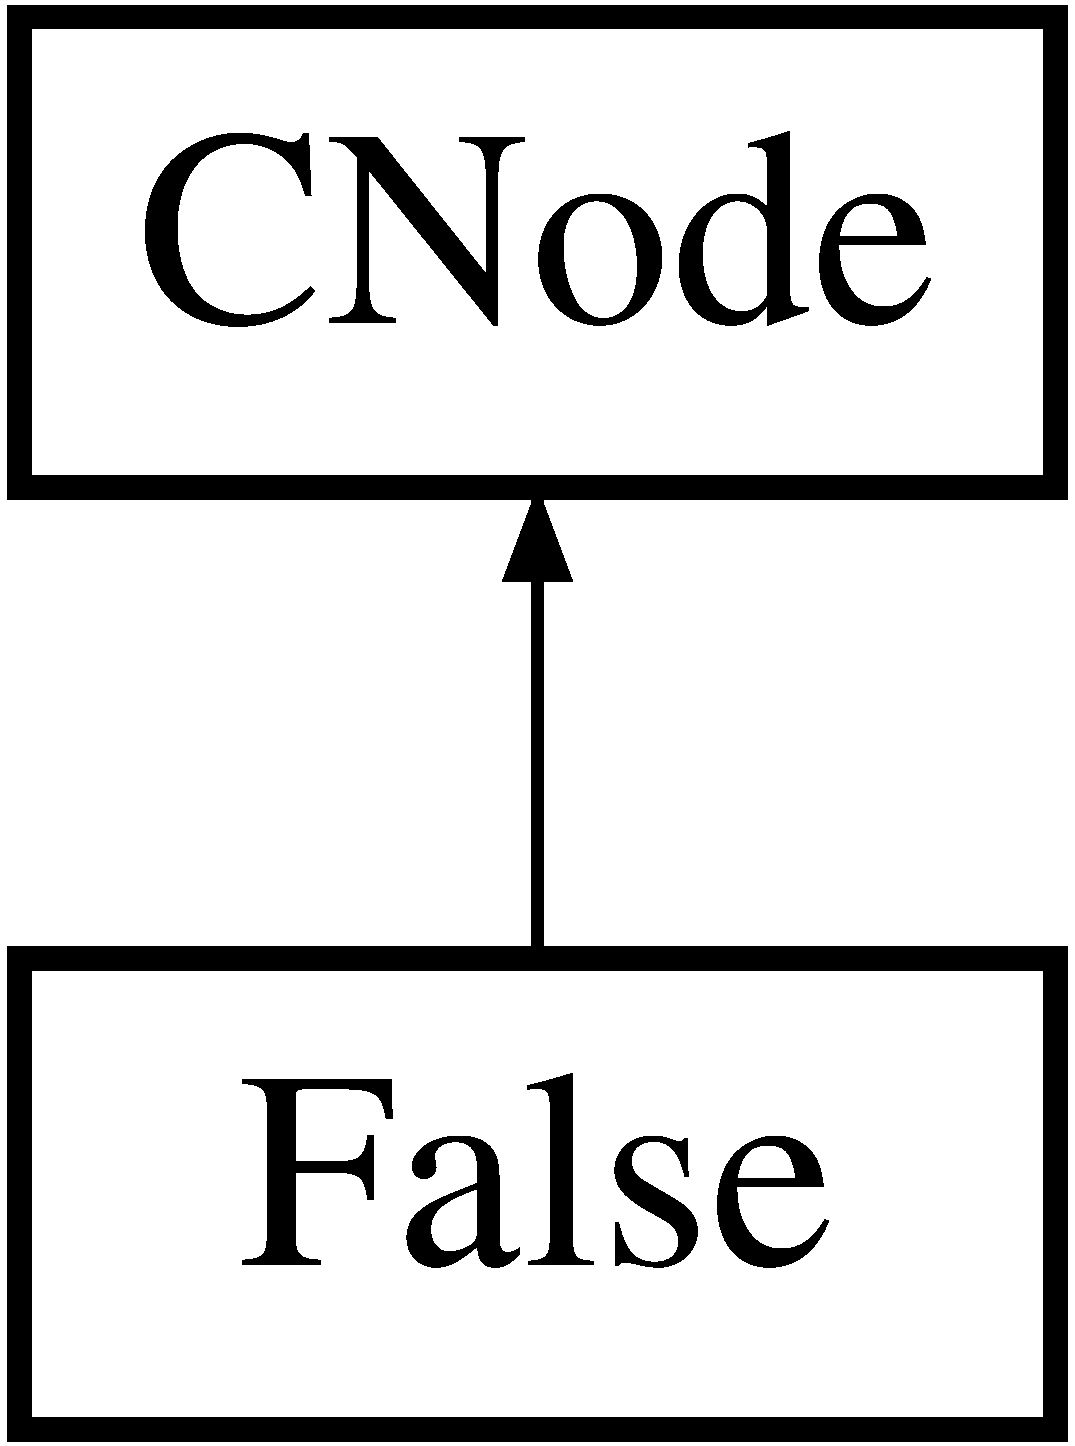
\includegraphics[height=2.000000cm]{classFalse}
\end{center}
\end{figure}
\subsection*{\-Public \-Member \-Functions}
\begin{DoxyCompactItemize}
\item 
\hypertarget{classFalse_aa5a4738c7d2296953282ead016ac6b25}{virtual bool {\bfseries operator==} (const \hyperlink{classCNode}{\-C\-Node} \&other)}\label{classFalse_aa5a4738c7d2296953282ead016ac6b25}

\item 
\hypertarget{classFalse_a1c34f63f8f6f3949f0ab9e44257b3061}{virtual \hyperlink{classCNode}{\-C\-Node} $\ast$ {\bfseries substitute} (map$<$ \hyperlink{classTerm}{\-Term} $\ast$, \hyperlink{classTerm}{\-Term} $\ast$ $>$ \&subs)}\label{classFalse_a1c34f63f8f6f3949f0ab9e44257b3061}

\item 
\hypertarget{classFalse_a1cae1258ee20b432f44bf20fb78ade0b}{virtual string {\bfseries to\-\_\-string} ()}\label{classFalse_a1cae1258ee20b432f44bf20fb78ade0b}

\end{DoxyCompactItemize}
\subsection*{\-Static \-Public \-Member \-Functions}
\begin{DoxyCompactItemize}
\item 
\hypertarget{classFalse_ae7d34903159164e27ac65c62660fc610}{static \hyperlink{classCNode}{\-C\-Node} $\ast$ {\bfseries make} ()}\label{classFalse_ae7d34903159164e27ac65c62660fc610}

\end{DoxyCompactItemize}
\subsection*{\-Friends}
\begin{DoxyCompactItemize}
\item 
\hypertarget{classFalse_ac98d07dd8f7b70e16ccb9a01abf56b9c}{class {\bfseries boost\-::serialization\-::access}}\label{classFalse_ac98d07dd8f7b70e16ccb9a01abf56b9c}

\item 
\hypertarget{classFalse_a0657a422d4ddc5f4a0ff56931b7d2767}{class {\bfseries \-C\-Node}}\label{classFalse_a0657a422d4ddc5f4a0ff56931b7d2767}

\end{DoxyCompactItemize}


\-The documentation for this class was generated from the following files\-:\begin{DoxyCompactItemize}
\item 
cnode/\-False.\-h\item 
cnode/\-False.\-cpp\end{DoxyCompactItemize}

\hypertarget{structfun__bg}{\section{fun\-\_\-bg \-Struct \-Reference}
\label{structfun__bg}\index{fun\-\_\-bg@{fun\-\_\-bg}}
}
\subsection*{\-Public \-Attributes}
\begin{DoxyCompactItemize}
\item 
\hypertarget{structfun__bg_ac08c75138f8571270e66c540873e3d5f}{\hyperlink{classCNode}{\-C\-Node} $\ast$ {\bfseries key}}\label{structfun__bg_ac08c75138f8571270e66c540873e3d5f}

\item 
\hypertarget{structfun__bg_a9e605822bd2112167a13fff953bb419c}{\hyperlink{classTerm}{\-Term} $\ast$ {\bfseries quantified\-\_\-var}}\label{structfun__bg_a9e605822bd2112167a13fff953bb419c}

\item 
\hypertarget{structfun__bg_a11758482a6c506138dfbebc9486a6eba}{\hyperlink{classCNode}{\-C\-Node} $\ast$ {\bfseries nc\-\_\-val}}\label{structfun__bg_a11758482a6c506138dfbebc9486a6eba}

\item 
\hypertarget{structfun__bg_a39d796262955c81e89ac9e51c03736e8}{\hyperlink{classCNode}{\-C\-Node} $\ast$ {\bfseries sc\-\_\-val}}\label{structfun__bg_a39d796262955c81e89ac9e51c03736e8}

\end{DoxyCompactItemize}


\-The documentation for this struct was generated from the following file\-:\begin{DoxyCompactItemize}
\item 
\-Constraint\-Solver.\-h\end{DoxyCompactItemize}

\hypertarget{classFunctionTerm}{\section{\-Function\-Term \-Class \-Reference}
\label{classFunctionTerm}\index{\-Function\-Term@{\-Function\-Term}}
}
\-Inheritance diagram for \-Function\-Term\-:\begin{figure}[H]
\begin{center}
\leavevmode
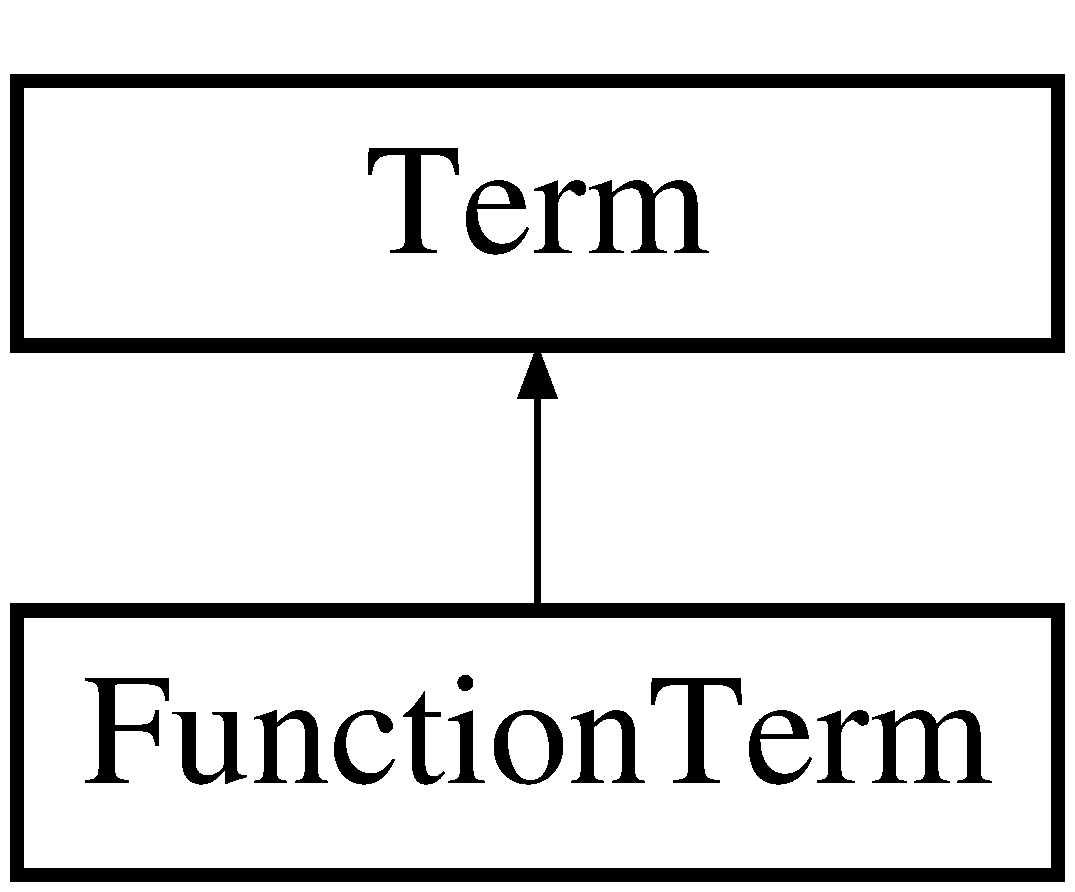
\includegraphics[height=2.000000cm]{classFunctionTerm}
\end{center}
\end{figure}
\subsection*{\-Public \-Member \-Functions}
\begin{DoxyCompactItemize}
\item 
\hypertarget{classFunctionTerm_a5d4e3e694d75d8431e7bf55092c37ce7}{{\footnotesize template$<$class Archive $>$ }\\void {\bfseries save} (\-Archive \&ar, const unsigned int version) const }\label{classFunctionTerm_a5d4e3e694d75d8431e7bf55092c37ce7}

\item 
\hypertarget{classFunctionTerm_a413d70e30ff5d361d676a13bd510224d}{{\footnotesize template$<$class Archive $>$ }\\void {\bfseries load} (\-Archive \&ar, const unsigned int version)}\label{classFunctionTerm_a413d70e30ff5d361d676a13bd510224d}

\item 
\hypertarget{classFunctionTerm_aea5a9451a9a792e9740ad7a655788610}{{\bfseries \-Function\-Term} (int id, const vector$<$ \hyperlink{classTerm}{\-Term} $\ast$ $>$ \&args, bool invertible, int attribute=0)}\label{classFunctionTerm_aea5a9451a9a792e9740ad7a655788610}

\item 
\hypertarget{classFunctionTerm_a16f50617f09e608064c08ea88ec12f10}{virtual bool {\bfseries operator==} (const \hyperlink{classTerm}{\-Term} \&other)}\label{classFunctionTerm_a16f50617f09e608064c08ea88ec12f10}

\item 
\hypertarget{classFunctionTerm_ae6cadfbb98234e9422e9e07240e6044a}{virtual string {\bfseries to\-\_\-string} ()}\label{classFunctionTerm_ae6cadfbb98234e9422e9e07240e6044a}

\item 
\hypertarget{classFunctionTerm_a1b81d3b0dd552eef335f6e12087bf5d0}{int {\bfseries get\-\_\-id} () const }\label{classFunctionTerm_a1b81d3b0dd552eef335f6e12087bf5d0}

\item 
\hypertarget{classFunctionTerm_a22fec1cbe07e0314fed0b388f37bd7c8}{bool {\bfseries is\-\_\-invertible} ()}\label{classFunctionTerm_a22fec1cbe07e0314fed0b388f37bd7c8}

\item 
\hypertarget{classFunctionTerm_ae527a349c1f27676e9d8c95129ba0630}{string {\bfseries get\-\_\-name} ()}\label{classFunctionTerm_ae527a349c1f27676e9d8c95129ba0630}

\item 
\hypertarget{classFunctionTerm_a9fc573a0638b61a2546273facd56741c}{virtual \hyperlink{classTerm}{\-Term} $\ast$ {\bfseries substitute} (map$<$ \hyperlink{classTerm}{\-Term} $\ast$, \hyperlink{classTerm}{\-Term} $\ast$ $>$ \&subs)}\label{classFunctionTerm_a9fc573a0638b61a2546273facd56741c}

\item 
\hypertarget{classFunctionTerm_a9ff7b53d253720ca7a465241b614f2bd}{const vector$<$ \hyperlink{classTerm}{\-Term} $\ast$ $>$ \& {\bfseries get\-\_\-args} ()}\label{classFunctionTerm_a9ff7b53d253720ca7a465241b614f2bd}

\item 
\hypertarget{classFunctionTerm_ac976c859fad01ce48128390f6a6fecb1}{int {\bfseries get\-\_\-id\-\_\-attribute} () const }\label{classFunctionTerm_ac976c859fad01ce48128390f6a6fecb1}

\end{DoxyCompactItemize}
\subsection*{\-Static \-Public \-Member \-Functions}
\begin{DoxyCompactItemize}
\item 
\hypertarget{classFunctionTerm_a475997b6b7d2a2ca4e80da2fa07f1543}{static \hyperlink{classTerm}{\-Term} $\ast$ {\bfseries make} (int id, vector$<$ \hyperlink{classTerm}{\-Term} $\ast$ $>$ \&args, bool invertible)}\label{classFunctionTerm_a475997b6b7d2a2ca4e80da2fa07f1543}

\item 
\hypertarget{classFunctionTerm_ac5092f73a70c2bd5c888dca2997e19b8}{static \hyperlink{classTerm}{\-Term} $\ast$ {\bfseries make} (string name, vector$<$ \hyperlink{classTerm}{\-Term} $\ast$ $>$ \&args, bool invertible)}\label{classFunctionTerm_ac5092f73a70c2bd5c888dca2997e19b8}

\end{DoxyCompactItemize}
\subsection*{\-Public \-Attributes}
\begin{DoxyCompactItemize}
\item 
\hypertarget{classFunctionTerm_a311b58312868fff403a0d1128f57d204}{int {\bfseries fun\-\_\-id}}\label{classFunctionTerm_a311b58312868fff403a0d1128f57d204}

\item 
\hypertarget{classFunctionTerm_a7794d59a801102a8447313d18be77afd}{vector$<$ \hyperlink{classTerm}{\-Term} $\ast$ $>$ {\bfseries args}}\label{classFunctionTerm_a7794d59a801102a8447313d18be77afd}

\item 
\hypertarget{classFunctionTerm_a4996a70d946b3d6af3ac586d6fcd3793}{bool {\bfseries invertible}}\label{classFunctionTerm_a4996a70d946b3d6af3ac586d6fcd3793}

\end{DoxyCompactItemize}
\subsection*{\-Protected \-Member \-Functions}
\begin{DoxyCompactItemize}
\item 
\hypertarget{classFunctionTerm_a7f1d077f0b9ce911ad615d7bd5ba3cac}{{\bfseries \-Function\-Term} (int id, \hyperlink{classTerm}{\-Term} $\ast$arg, bool invertible, int attribute=0)}\label{classFunctionTerm_a7f1d077f0b9ce911ad615d7bd5ba3cac}

\item 
\hypertarget{classFunctionTerm_a6170213bd26f3b728776c1f7fe87b3d7}{{\bfseries \-Function\-Term} (int id, \hyperlink{classTerm}{\-Term} $\ast$arg1, \hyperlink{classTerm}{\-Term} $\ast$arg2, bool invertible, int attribute=0)}\label{classFunctionTerm_a6170213bd26f3b728776c1f7fe87b3d7}

\item 
\hypertarget{classFunctionTerm_aeef76615552e8a539b1892e94ed1991b}{void {\bfseries compute\-\_\-hash\-\_\-code} ()}\label{classFunctionTerm_aeef76615552e8a539b1892e94ed1991b}

\end{DoxyCompactItemize}
\subsection*{\-Friends}
\begin{DoxyCompactItemize}
\item 
\hypertarget{classFunctionTerm_adebe709d4e5fe83b3c51c5605f625287}{class {\bfseries \-Address}}\label{classFunctionTerm_adebe709d4e5fe83b3c51c5605f625287}

\item 
\hypertarget{classFunctionTerm_aa1502d55736d0d860b8c757993f344f4}{class {\bfseries \-String\-Literal}}\label{classFunctionTerm_aa1502d55736d0d860b8c757993f344f4}

\item 
\hypertarget{classFunctionTerm_a758f8e4b1f004f64affee9def22769ff}{class {\bfseries \-Program\-Function}}\label{classFunctionTerm_a758f8e4b1f004f64affee9def22769ff}

\item 
\hypertarget{classFunctionTerm_aeafbb0e82d7e2b2377f7dc4a4df76254}{class {\bfseries \-Type\-Constant}}\label{classFunctionTerm_aeafbb0e82d7e2b2377f7dc4a4df76254}

\item 
\hypertarget{classFunctionTerm_ac98d07dd8f7b70e16ccb9a01abf56b9c}{class {\bfseries boost\-::serialization\-::access}}\label{classFunctionTerm_ac98d07dd8f7b70e16ccb9a01abf56b9c}

\end{DoxyCompactItemize}


\-The documentation for this class was generated from the following files\-:\begin{DoxyCompactItemize}
\item 
term/\-Function\-Term.\-h\item 
term/\-Function\-Term.\-cpp\end{DoxyCompactItemize}

\hypertarget{structHash}{\section{\-Hash$<$ \-K $>$ \-Struct \-Template \-Reference}
\label{structHash}\index{\-Hash$<$ K $>$@{\-Hash$<$ K $>$}}
}
\subsection*{\-Public \-Member \-Functions}
\begin{DoxyCompactItemize}
\item 
\hypertarget{structHash_a4a1c142a06baadd553bb81951fe7fa2e}{uint32\-\_\-t {\bfseries operator()} (const \-K \&k) const }\label{structHash_a4a1c142a06baadd553bb81951fe7fa2e}

\end{DoxyCompactItemize}
\subsubsection*{template$<$class K$>$ struct Hash$<$ K $>$}



\-The documentation for this struct was generated from the following file\-:\begin{DoxyCompactItemize}
\item 
sat-\/solver/\-Map.\-h\end{DoxyCompactItemize}

\hypertarget{classHeap}{\section{\-Heap$<$ \-Comp $>$ \-Class \-Template \-Reference}
\label{classHeap}\index{\-Heap$<$ Comp $>$@{\-Heap$<$ Comp $>$}}
}
\subsection*{\-Public \-Member \-Functions}
\begin{DoxyCompactItemize}
\item 
\hypertarget{classHeap_acec83ccbc9fd67b1e2fc9f182bd59317}{{\bfseries \-Heap} (const \-Comp \&c)}\label{classHeap_acec83ccbc9fd67b1e2fc9f182bd59317}

\item 
\hypertarget{classHeap_a1df0c4d5ea60b18a2f3e1c3ff5655c44}{int {\bfseries size} () const }\label{classHeap_a1df0c4d5ea60b18a2f3e1c3ff5655c44}

\item 
\hypertarget{classHeap_a35e73481fcd46b6be1e1f80a47507a50}{bool {\bfseries empty} () const }\label{classHeap_a35e73481fcd46b6be1e1f80a47507a50}

\item 
\hypertarget{classHeap_a4b4012639a72a9e763e370c414c24167}{bool {\bfseries in\-Heap} (int n) const }\label{classHeap_a4b4012639a72a9e763e370c414c24167}

\item 
\hypertarget{classHeap_ad4b243701b1944b645ec06a09a4a497a}{int {\bfseries operator\mbox{[}$\,$\mbox{]}} (int index) const }\label{classHeap_ad4b243701b1944b645ec06a09a4a497a}

\item 
\hypertarget{classHeap_a7766a74f069e51d829419b6bca3f5134}{void {\bfseries decrease} (int n)}\label{classHeap_a7766a74f069e51d829419b6bca3f5134}

\item 
\hypertarget{classHeap_a6f5ab48e1b3b99e704080628ce6fc666}{void {\bfseries increase\-\_\-} (int n)}\label{classHeap_a6f5ab48e1b3b99e704080628ce6fc666}

\item 
\hypertarget{classHeap_a078b00c9c59a7d46e4daa48ad81527a0}{void {\bfseries insert} (int n)}\label{classHeap_a078b00c9c59a7d46e4daa48ad81527a0}

\item 
\hypertarget{classHeap_a6ae9aab43f5e2ec23722a20113b802e4}{void {\bfseries init\-\_\-identical} (int n)}\label{classHeap_a6ae9aab43f5e2ec23722a20113b802e4}

\item 
\hypertarget{classHeap_a3b6378eebf64ba1fe99b139611ed2bbf}{int {\bfseries remove\-Min} ()}\label{classHeap_a3b6378eebf64ba1fe99b139611ed2bbf}

\item 
\hypertarget{classHeap_a3018b631f27fc84c7db692126e985e41}{void {\bfseries clear} (bool dealloc=false)}\label{classHeap_a3018b631f27fc84c7db692126e985e41}

\item 
\hypertarget{classHeap_a5819cfc5b50061d1e288881d3466f2ec}{void {\bfseries update} (int n)}\label{classHeap_a5819cfc5b50061d1e288881d3466f2ec}

\item 
\hypertarget{classHeap_ae0fad85e429c9eb0bf1d4e3d93d4fbbf}{{\footnotesize template$<$class F $>$ }\\void {\bfseries filter} (const \-F \&filt)}\label{classHeap_ae0fad85e429c9eb0bf1d4e3d93d4fbbf}

\item 
\hypertarget{classHeap_a2ecafb1795e9ea3fc9091db6884f2695}{bool {\bfseries heap\-Property} () const }\label{classHeap_a2ecafb1795e9ea3fc9091db6884f2695}

\item 
\hypertarget{classHeap_ab0e6f79043278fd47a609ccd864ef70c}{void {\bfseries set\-Bounds} (int n)}\label{classHeap_ab0e6f79043278fd47a609ccd864ef70c}

\item 
\hypertarget{classHeap_a8a82b5a31dc0ec7cb0cb729d4ac606b0}{void {\bfseries increase} (int n)}\label{classHeap_a8a82b5a31dc0ec7cb0cb729d4ac606b0}

\item 
\hypertarget{classHeap_a7e9f205407d038020f354eb67f09b7b4}{int {\bfseries getmin} ()}\label{classHeap_a7e9f205407d038020f354eb67f09b7b4}

\end{DoxyCompactItemize}
\subsubsection*{template$<$class \-Comp$>$ class Heap$<$ Comp $>$}



\-The documentation for this class was generated from the following file\-:\begin{DoxyCompactItemize}
\item 
sat-\/solver/\-Heap.\-h\end{DoxyCompactItemize}

\hypertarget{classILPLeaf}{\section{\-I\-L\-P\-Leaf \-Class \-Reference}
\label{classILPLeaf}\index{\-I\-L\-P\-Leaf@{\-I\-L\-P\-Leaf}}
}
\-Inheritance diagram for \-I\-L\-P\-Leaf\-:\begin{figure}[H]
\begin{center}
\leavevmode
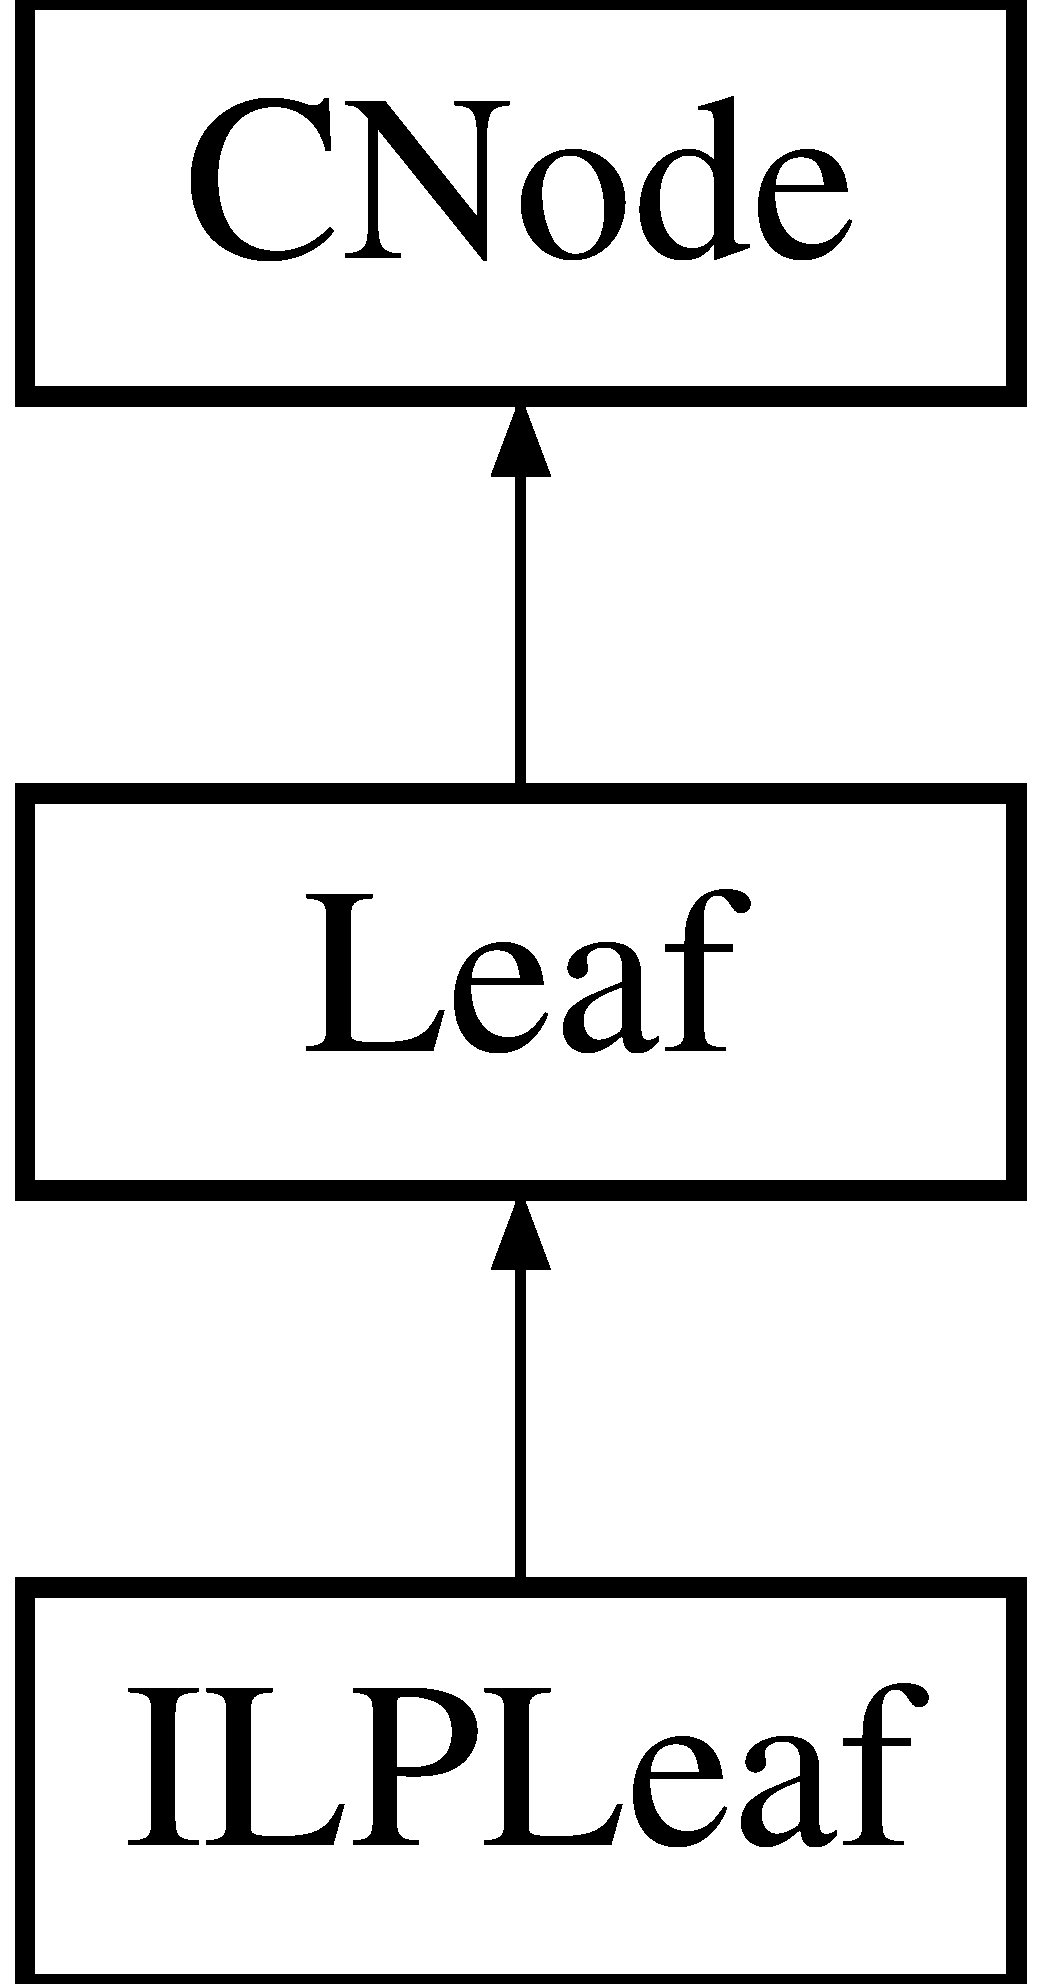
\includegraphics[height=3.000000cm]{classILPLeaf}
\end{center}
\end{figure}
\subsection*{\-Public \-Member \-Functions}
\begin{DoxyCompactItemize}
\item 
\hypertarget{classILPLeaf_a3683eed8b33a76cdd8a2a3e521029b28}{virtual bool {\bfseries operator==} (const \hyperlink{classCNode}{\-C\-Node} \&other)}\label{classILPLeaf_a3683eed8b33a76cdd8a2a3e521029b28}

\item 
\hypertarget{classILPLeaf_a888f4656b61bf03f7c2c7d3c7d45e7e2}{virtual string {\bfseries to\-\_\-string} ()}\label{classILPLeaf_a888f4656b61bf03f7c2c7d3c7d45e7e2}

\item 
\hypertarget{classILPLeaf_a0a694ab27b8c6a5a45926b97f4f60c51}{ilp\-\_\-leaf\-\_\-type {\bfseries get\-\_\-operator} ()}\label{classILPLeaf_a0a694ab27b8c6a5a45926b97f4f60c51}

\item 
\hypertarget{classILPLeaf_a601e640ff15c02f3a7c0ee5f4dc25a82}{const map$<$ \hyperlink{classTerm}{\-Term} $\ast$, long int $>$ \& {\bfseries get\-\_\-elems} ()}\label{classILPLeaf_a601e640ff15c02f3a7c0ee5f4dc25a82}

\item 
\hypertarget{classILPLeaf_a9ce63fa37098afe3d590a50d5862b8bc}{long int {\bfseries get\-\_\-constant} ()}\label{classILPLeaf_a9ce63fa37098afe3d590a50d5862b8bc}

\item 
\hypertarget{classILPLeaf_aec0b09c10a2f2e32609db6faf1e064bd}{long {\bfseries get\-\_\-coefficient} (\hyperlink{classTerm}{\-Term} $\ast$t)}\label{classILPLeaf_aec0b09c10a2f2e32609db6faf1e064bd}

\item 
\hypertarget{classILPLeaf_aaec744311d63d28f58fd130c218d828c}{bool {\bfseries contains\-\_\-elem} (\hyperlink{classTerm}{\-Term} $\ast$t)}\label{classILPLeaf_aaec744311d63d28f58fd130c218d828c}

\item 
\hypertarget{classILPLeaf_a456ddb011ba699d884e037c2054ac881}{\hyperlink{classCNode}{\-C\-Node} $\ast$ {\bfseries remove\-\_\-elem} (\hyperlink{classTerm}{\-Term} $\ast$t)}\label{classILPLeaf_a456ddb011ba699d884e037c2054ac881}

\item 
\hypertarget{classILPLeaf_abbaa583ce97c9061e3c8f2dff10884fc}{\hyperlink{classCNode}{\-C\-Node} $\ast$ {\bfseries negate} (bool remove\-\_\-all\-\_\-negations=false)}\label{classILPLeaf_abbaa583ce97c9061e3c8f2dff10884fc}

\item 
\hypertarget{classILPLeaf_a4fd0cbc6c3ee5f89b7e7a1146b39b6c6}{virtual \hyperlink{classCNode}{\-C\-Node} $\ast$ {\bfseries substitute} (map$<$ \hyperlink{classTerm}{\-Term} $\ast$, \hyperlink{classTerm}{\-Term} $\ast$ $>$ \&subs)}\label{classILPLeaf_a4fd0cbc6c3ee5f89b7e7a1146b39b6c6}

\item 
\hypertarget{classILPLeaf_a1351d142419128c4da2cfde59970f5e2}{\hyperlink{classCNode}{\-C\-Node} $\ast$ {\bfseries multiply} (long int factor)}\label{classILPLeaf_a1351d142419128c4da2cfde59970f5e2}

\item 
\hypertarget{classILPLeaf_a2a2a3f3c521e9668a3b74e4914ca1819}{\hyperlink{classCNode}{\-C\-Node} $\ast$ {\bfseries add} (\hyperlink{classILPLeaf}{\-I\-L\-P\-Leaf} $\ast$other)}\label{classILPLeaf_a2a2a3f3c521e9668a3b74e4914ca1819}

\item 
\hypertarget{classILPLeaf_ae866511969891fe9d213038e900cfc25}{string {\bfseries pretty\-\_\-print\-\_\-ilp} (bool neg)}\label{classILPLeaf_ae866511969891fe9d213038e900cfc25}

\item 
\hypertarget{classILPLeaf_af1aed72a3fcf4662a7c60e240fe368cc}{virtual \hyperlink{classCNode}{\-C\-Node} $\ast$ {\bfseries divide} (long int c, \hyperlink{classTerm}{\-Term} $\ast$t)}\label{classILPLeaf_af1aed72a3fcf4662a7c60e240fe368cc}

\end{DoxyCompactItemize}
\subsection*{\-Static \-Public \-Member \-Functions}
\begin{DoxyCompactItemize}
\item 
\hypertarget{classILPLeaf_abf0eed608f5cd1950919b43883207323}{static \hyperlink{classCNode}{\-C\-Node} $\ast$ {\bfseries make} (ilp\-\_\-leaf\-\_\-type kind, const map$<$ \hyperlink{classTerm}{\-Term} $\ast$, long int $>$ \&elems, long int constant)}\label{classILPLeaf_abf0eed608f5cd1950919b43883207323}

\item 
\hypertarget{classILPLeaf_a643b96a6a598b0ab389feb2f32a91470}{static \hyperlink{classCNode}{\-C\-Node} $\ast$ {\bfseries make} (\hyperlink{classTerm}{\-Term} $\ast$t1, \hyperlink{classTerm}{\-Term} $\ast$t2, ilp\-\_\-leaf\-\_\-type kind)}\label{classILPLeaf_a643b96a6a598b0ab389feb2f32a91470}

\item 
\hypertarget{classILPLeaf_a115dddc2676faf2f1322c27ab2ac57d0}{static string {\bfseries ilp\-\_\-leaf\-\_\-type\-\_\-to\-\_\-string} (ilp\-\_\-leaf\-\_\-type t)}\label{classILPLeaf_a115dddc2676faf2f1322c27ab2ac57d0}

\end{DoxyCompactItemize}
\subsection*{\-Protected \-Member \-Functions}
\begin{DoxyCompactItemize}
\item 
\hypertarget{classILPLeaf_acd83ccdf9b353bf2ffb97f0e67238981}{{\bfseries \-I\-L\-P\-Leaf} (ilp\-\_\-leaf\-\_\-type kind, const map$<$ \hyperlink{classTerm}{\-Term} $\ast$, long int $>$ \&elems, long int constant)}\label{classILPLeaf_acd83ccdf9b353bf2ffb97f0e67238981}

\end{DoxyCompactItemize}
\subsection*{\-Friends}
\begin{DoxyCompactItemize}
\item 
\hypertarget{classILPLeaf_ac98d07dd8f7b70e16ccb9a01abf56b9c}{class {\bfseries boost\-::serialization\-::access}}\label{classILPLeaf_ac98d07dd8f7b70e16ccb9a01abf56b9c}

\end{DoxyCompactItemize}


\-The documentation for this class was generated from the following files\-:\begin{DoxyCompactItemize}
\item 
cnode/\-I\-L\-P\-Leaf.\-h\item 
cnode/\-I\-L\-P\-Leaf.\-cpp\end{DoxyCompactItemize}

\hypertarget{classILPQuery}{\section{\-I\-L\-P\-Query \-Class \-Reference}
\label{classILPQuery}\index{\-I\-L\-P\-Query@{\-I\-L\-P\-Query}}
}
\subsection*{\-Public \-Member \-Functions}
\begin{DoxyCompactItemize}
\item 
\hypertarget{classILPQuery_a6e1f24a8f3c18f0ec9f174e3e675a7d5}{{\bfseries \-I\-L\-P\-Query} (\hyperlink{classTerm}{\-Term} $\ast$rhs, \hyperlink{classTerm}{\-Term} $\ast$lhs)}\label{classILPQuery_a6e1f24a8f3c18f0ec9f174e3e675a7d5}

\item 
\hypertarget{classILPQuery_abbcb314b455ec2954fbe25915d1c50c4}{string {\bfseries to\-\_\-string} ()}\label{classILPQuery_abbcb314b455ec2954fbe25915d1c50c4}

\end{DoxyCompactItemize}
\subsection*{\-Public \-Attributes}
\begin{DoxyCompactItemize}
\item 
\hypertarget{classILPQuery_aa6d087d78bb93e1ad5ab6c1dda0ee56d}{\hyperlink{classTerm}{\-Term} $\ast$ {\bfseries t1}}\label{classILPQuery_aa6d087d78bb93e1ad5ab6c1dda0ee56d}

\item 
\hypertarget{classILPQuery_a5360d1ed1edda5715ef417bde6bf31dd}{\hyperlink{classTerm}{\-Term} $\ast$ {\bfseries t2}}\label{classILPQuery_a5360d1ed1edda5715ef417bde6bf31dd}

\end{DoxyCompactItemize}


\-The documentation for this class was generated from the following files\-:\begin{DoxyCompactItemize}
\item 
solver/\-Interaction\-Manager.\-h\item 
solver/\-Interaction\-Manager.\-cpp\end{DoxyCompactItemize}

\hypertarget{classInteractionManager}{\section{\-Interaction\-Manager \-Class \-Reference}
\label{classInteractionManager}\index{\-Interaction\-Manager@{\-Interaction\-Manager}}
}
\subsection*{\-Public \-Member \-Functions}
\begin{DoxyCompactItemize}
\item 
\hypertarget{classInteractionManager_a48325cce50121fb4263f9104e0c7803f}{{\bfseries \-Interaction\-Manager} (\hyperlink{classClauseSolve}{\-Clause\-Solve} $\ast$s, set$<$ \hyperlink{classTerm}{\-Term} $\ast$ $>$ \&equality\-\_\-terms, set$<$ int $>$ \&function\-\_\-terms)}\label{classInteractionManager_a48325cce50121fb4263f9104e0c7803f}

\item 
\hypertarget{classInteractionManager_a93d127911d029b27977b3fcc442c375a}{bool {\bfseries add\-\_\-inferred\-\_\-equalities} ()}\label{classInteractionManager_a93d127911d029b27977b3fcc442c375a}

\item 
\hypertarget{classInteractionManager_a45eded00bd7b495ffd84f9a39b2cd649}{bool {\bfseries add\-\_\-inferred\-\_\-inequalities} ()}\label{classInteractionManager_a45eded00bd7b495ffd84f9a39b2cd649}

\item 
\hypertarget{classInteractionManager_a6e274b0bb9a96546781929f5175b43e8}{void {\bfseries build\-\_\-queries} ()}\label{classInteractionManager_a6e274b0bb9a96546781929f5175b43e8}

\item 
\hypertarget{classInteractionManager_a528262e6fa3c668032ee3ffd264e2767}{set$<$ \hyperlink{classILPQuery}{\-I\-L\-P\-Query} $\ast$ $>$ \& {\bfseries get\-\_\-queries} ()}\label{classInteractionManager_a528262e6fa3c668032ee3ffd264e2767}

\item 
\hypertarget{classInteractionManager_a32feeadb0b83bb4b14b944a144ce9035}{set$<$ \hyperlink{classILPQuery}{\-I\-L\-P\-Query} $\ast$ $>$ \& {\bfseries refine\-\_\-queries} ()}\label{classInteractionManager_a32feeadb0b83bb4b14b944a144ce9035}

\item 
\hypertarget{classInteractionManager_a95aad63b3dcf27795fa9b60cc076f974}{string {\bfseries queries\-\_\-to\-\_\-string} ()}\label{classInteractionManager_a95aad63b3dcf27795fa9b60cc076f974}

\end{DoxyCompactItemize}


\-The documentation for this class was generated from the following files\-:\begin{DoxyCompactItemize}
\item 
solver/\-Interaction\-Manager.\-h\item 
solver/\-Interaction\-Manager.\-cpp\end{DoxyCompactItemize}

\hypertarget{classLeaf}{\section{\-Leaf \-Class \-Reference}
\label{classLeaf}\index{\-Leaf@{\-Leaf}}
}
\-Inheritance diagram for \-Leaf\-:\begin{figure}[H]
\begin{center}
\leavevmode
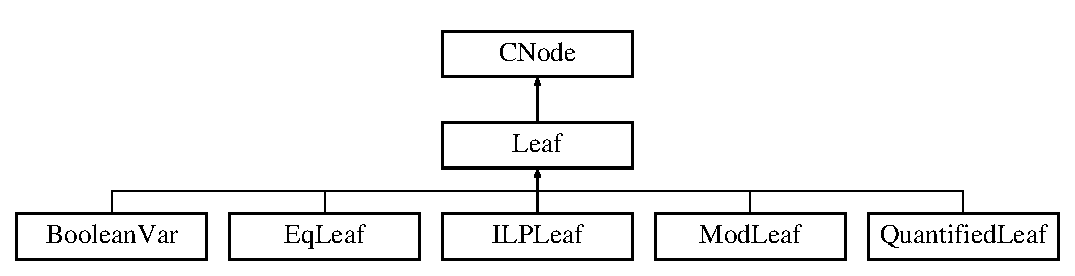
\includegraphics[height=3.000000cm]{classLeaf}
\end{center}
\end{figure}
\subsection*{\-Public \-Member \-Functions}
\begin{DoxyCompactItemize}
\item 
\hypertarget{classLeaf_aefbb7d9d2a72b85db191acbe798b6787}{virtual string {\bfseries to\-\_\-string} ()=0}\label{classLeaf_aefbb7d9d2a72b85db191acbe798b6787}

\end{DoxyCompactItemize}
\subsection*{\-Friends}
\begin{DoxyCompactItemize}
\item 
\hypertarget{classLeaf_ac98d07dd8f7b70e16ccb9a01abf56b9c}{class {\bfseries boost\-::serialization\-::access}}\label{classLeaf_ac98d07dd8f7b70e16ccb9a01abf56b9c}

\end{DoxyCompactItemize}


\-The documentation for this class was generated from the following files\-:\begin{DoxyCompactItemize}
\item 
cnode/\-Leaf.\-h\item 
cnode/\-Leaf.\-cpp\end{DoxyCompactItemize}

\hypertarget{structLessThan__default}{\section{\-Less\-Than\-\_\-default$<$ \-T $>$ \-Struct \-Template \-Reference}
\label{structLessThan__default}\index{\-Less\-Than\-\_\-default$<$ T $>$@{\-Less\-Than\-\_\-default$<$ T $>$}}
}
\subsection*{\-Public \-Member \-Functions}
\begin{DoxyCompactItemize}
\item 
\hypertarget{structLessThan__default_a0888e32196c15a7b2a0813d56fd3276b}{bool {\bfseries operator()} (\-T x, \-T y)}\label{structLessThan__default_a0888e32196c15a7b2a0813d56fd3276b}

\end{DoxyCompactItemize}
\subsubsection*{template$<$class T$>$ struct Less\-Than\-\_\-default$<$ T $>$}



\-The documentation for this struct was generated from the following file\-:\begin{DoxyCompactItemize}
\item 
sat-\/solver/\-Sort.\-h\end{DoxyCompactItemize}

\hypertarget{classMap}{\section{\-Map$<$ \-K, \-D, \-H, \-E $>$ \-Class \-Template \-Reference}
\label{classMap}\index{\-Map$<$ K, D, H, E $>$@{\-Map$<$ K, D, H, E $>$}}
}
\subsection*{\-Classes}
\begin{DoxyCompactItemize}
\item 
struct {\bfseries \-Pair}
\end{DoxyCompactItemize}
\subsection*{\-Public \-Member \-Functions}
\begin{DoxyCompactItemize}
\item 
\hypertarget{classMap_ae414440bb0972d00e2ad5ca4d56342b8}{{\bfseries \-Map} (const \-H \&h, const \-E \&e)}\label{classMap_ae414440bb0972d00e2ad5ca4d56342b8}

\item 
\hypertarget{classMap_ac50d9fbcde7f9bfb8532e29c1338a93b}{void {\bfseries insert} (const \-K \&k, const \-D \&d)}\label{classMap_ac50d9fbcde7f9bfb8532e29c1338a93b}

\item 
\hypertarget{classMap_a7ff0932fba67aec07797962f6189c300}{bool {\bfseries peek} (const \-K \&k, \-D \&d)}\label{classMap_a7ff0932fba67aec07797962f6189c300}

\item 
\hypertarget{classMap_a364147a784045f445ed41ebf3e2df29c}{void {\bfseries remove} (const \-K \&k)}\label{classMap_a364147a784045f445ed41ebf3e2df29c}

\item 
\hypertarget{classMap_af4e6d1eb23e08786d2f790ef86ebff2d}{void {\bfseries clear} ()}\label{classMap_af4e6d1eb23e08786d2f790ef86ebff2d}

\end{DoxyCompactItemize}
\subsubsection*{template$<$class \-K, class \-D, class \-H = \-Hash$<$\-K$>$, class \-E = \-Equal$<$\-K$>$$>$ class Map$<$ K, D, H, E $>$}



\-The documentation for this class was generated from the following file\-:\begin{DoxyCompactItemize}
\item 
sat-\/solver/\-Map.\-h\end{DoxyCompactItemize}

\hypertarget{classmatrix}{\section{matrix \-Class \-Reference}
\label{classmatrix}\index{matrix@{matrix}}
}
\subsection*{\-Public \-Member \-Functions}
\begin{DoxyCompactItemize}
\item 
\hypertarget{classmatrix_a3c6fcf718dcee66b64c02a49fc95d453}{{\bfseries matrix} (int rows, int num\-\_\-vars, vector$<$ string $>$ $\ast$vars)}\label{classmatrix_a3c6fcf718dcee66b64c02a49fc95d453}

\item 
\hypertarget{classmatrix_a9e077c39ae45c2912bba77eb93a296d1}{{\bfseries matrix} (int rows, int cols)}\label{classmatrix_a9e077c39ae45c2912bba77eb93a296d1}

\item 
\hypertarget{classmatrix_a5fd2825c8ca21d023209845f31becc9f}{int {\bfseries num\-\_\-rows} ()}\label{classmatrix_a5fd2825c8ca21d023209845f31becc9f}

\item 
\hypertarget{classmatrix_ac3244bb0c7739890bf309d216e23a055}{int {\bfseries num\-\_\-vars} ()}\label{classmatrix_ac3244bb0c7739890bf309d216e23a055}

\item 
\hypertarget{classmatrix_a04f1d120c6ad17cac1e15ad26e07fb47}{int {\bfseries num\-\_\-cols} ()}\label{classmatrix_a04f1d120c6ad17cac1e15ad26e07fb47}

\item 
\hypertarget{classmatrix_a48c71476541b8b226973016f146484b9}{{\bfseries matrix} (const \hyperlink{classmatrix}{matrix} \&other, int new\-\_\-rows=-\/1)}\label{classmatrix_a48c71476541b8b226973016f146484b9}

\item 
\hypertarget{classmatrix_a01d679e9b5a43a8db13eef2ea7c4653c}{void {\bfseries simplify\-\_\-matrix} ()}\label{classmatrix_a01d679e9b5a43a8db13eef2ea7c4653c}

\item 
\hypertarget{classmatrix_ab72918afc60a2f4ec582de7f89b582ac}{void {\bfseries set} (int r, int c, \hyperlink{classbignum}{bignum} v)}\label{classmatrix_ab72918afc60a2f4ec582de7f89b582ac}

\item 
\hypertarget{classmatrix_a392d201cede47f99cebf3fe683ac1db0}{void {\bfseries set} (int r, int c, long int i)}\label{classmatrix_a392d201cede47f99cebf3fe683ac1db0}

\item 
\hypertarget{classmatrix_af48c96d206d8007ec88dadba77529fde}{\hyperlink{classbignum}{bignum} {\bfseries get} (int r, int c)}\label{classmatrix_af48c96d206d8007ec88dadba77529fde}

\item 
\hypertarget{classmatrix_a7662abc6ef708f9ef6585628091e0968}{void {\bfseries multiply\-\_\-row} (int r, \hyperlink{classbignum}{bignum} f)}\label{classmatrix_a7662abc6ef708f9ef6585628091e0968}

\item 
\hypertarget{classmatrix_a52330a6367fbef44d008000a6e8e22e7}{void {\bfseries flip\-\_\-row\-\_\-sign} (int r)}\label{classmatrix_a52330a6367fbef44d008000a6e8e22e7}

\item 
\hypertarget{classmatrix_a4fb197f10e386909e2c990e2171ceeca}{void {\bfseries divide\-\_\-row} (int r, \hyperlink{classbignum}{bignum} f)}\label{classmatrix_a4fb197f10e386909e2c990e2171ceeca}

\item 
\hypertarget{classmatrix_a4cfb024cd09bd851fc00a453ca315960}{void {\bfseries add\-\_\-row} (int r, \hyperlink{classbignum}{bignum} f)}\label{classmatrix_a4cfb024cd09bd851fc00a453ca315960}

\item 
\hypertarget{classmatrix_a830c40d1d028da32195d647923865ad2}{void {\bfseries delete\-\_\-bigrow} (int r)}\label{classmatrix_a830c40d1d028da32195d647923865ad2}

\item 
\hypertarget{classmatrix_ab6bf699286d426f4e768facdef4808e8}{string {\bfseries to\-\_\-string} ()}\label{classmatrix_ab6bf699286d426f4e768facdef4808e8}

\item 
\hypertarget{classmatrix_a77d3e3ff3d4a887509d2f4fc2b854cd2}{\hyperlink{classbignum}{bignum} {\bfseries get\-\_\-coef\-\_\-gcd} (int r)}\label{classmatrix_a77d3e3ff3d4a887509d2f4fc2b854cd2}

\item 
\hypertarget{classmatrix_aa08a8b818aff21a0b111a247661f6ec0}{vector$<$ string $>$ \& {\bfseries get\-\_\-vars} ()}\label{classmatrix_aa08a8b818aff21a0b111a247661f6ec0}

\item 
\hypertarget{classmatrix_aa2d436298cfd2e6d1fb0dbd3551c83ad}{int {\bfseries get\-\_\-pivot} (int r)}\label{classmatrix_aa2d436298cfd2e6d1fb0dbd3551c83ad}

\item 
\hypertarget{classmatrix_a86510224f830f6c92ca415df037727aa}{\hyperlink{classbignum}{bignum} {\bfseries get\-\_\-constant} (int r)}\label{classmatrix_a86510224f830f6c92ca415df037727aa}

\item 
\hypertarget{classmatrix_a806dfaa0efa6f3b3b89aaad05265782a}{void {\bfseries set\-\_\-constant} (int r, \hyperlink{classbignum}{bignum} b)}\label{classmatrix_a806dfaa0efa6f3b3b89aaad05265782a}

\item 
\hypertarget{classmatrix_accea607c2f03c6b146dbbe9e7485f442}{void {\bfseries set\-\_\-pivot} (int r, int p)}\label{classmatrix_accea607c2f03c6b146dbbe9e7485f442}

\item 
\hypertarget{classmatrix_a60f033001cb12ece250d24e7d4a2877d}{int {\bfseries get\-\_\-first\-\_\-positive\-\_\-index} (int r)}\label{classmatrix_a60f033001cb12ece250d24e7d4a2877d}

\item 
\hypertarget{classmatrix_ad37aac40673b23a7a51e1442ce324cf8}{void {\bfseries pivot} (int pivot\-\_\-row, int pivot\-\_\-index, bool simplify=true)}\label{classmatrix_ad37aac40673b23a7a51e1442ce324cf8}

\item 
\hypertarget{classmatrix_aab888ed9660b734a8e14ae8db9ebf320}{void {\bfseries multiply} (\hyperlink{classmatrix}{matrix} \&op, \hyperlink{classmatrix}{matrix} \&result)}\label{classmatrix_aab888ed9660b734a8e14ae8db9ebf320}

\item 
\hypertarget{classmatrix_a1b0be29630a770624c7ee93641547d55}{\hyperlink{classbignum}{bignum} {\bfseries dot\-\_\-product} (int r, int cc, \hyperlink{classmatrix}{matrix} \&op)}\label{classmatrix_a1b0be29630a770624c7ee93641547d55}

\item 
\hypertarget{classmatrix_a098decbf12b8c5b66575d17fce4c7f1f}{void {\bfseries compute\-\_\-redundant\-\_\-rows} (std\-::set$<$ int $>$ \&red\-\_\-rows)}\label{classmatrix_a098decbf12b8c5b66575d17fce4c7f1f}

\item 
\hypertarget{classmatrix_a5323b59c82073276e1facbd22abcf8f1}{\hyperlink{classbignum}{bignum} {\bfseries invert} (\hyperlink{classmatrix}{matrix} \&result)}\label{classmatrix_a5323b59c82073276e1facbd22abcf8f1}

\item 
\hypertarget{classmatrix_a3a708f73636f1302b91c99183381b443}{void {\bfseries vector\-\_\-multiply} (\hyperlink{classbignum}{bignum} $\ast$b, \hyperlink{classbignum}{bignum} $\ast$res)}\label{classmatrix_a3a708f73636f1302b91c99183381b443}

\item 
\hypertarget{classmatrix_ac304b39759d0551990b3da0f00309cfa}{void {\bfseries row\-\_\-vector\-\_\-multiply} (\hyperlink{classbignum}{bignum} $\ast$b, \hyperlink{classbignum}{bignum} $\ast$res)}\label{classmatrix_ac304b39759d0551990b3da0f00309cfa}

\end{DoxyCompactItemize}
\subsection*{\-Protected \-Attributes}
\begin{DoxyCompactItemize}
\item 
\hypertarget{classmatrix_aef4166e34912a3aa6a3a094bc04e3c40}{\hyperlink{uniondata__type}{data\-\_\-type} $\ast$ {\bfseries dmatrix}}\label{classmatrix_aef4166e34912a3aa6a3a094bc04e3c40}

\item 
\hypertarget{classmatrix_a4b1510b3427815ae114b66d1bea22ca3}{const int {\bfseries rows}}\label{classmatrix_a4b1510b3427815ae114b66d1bea22ca3}

\item 
\hypertarget{classmatrix_a2a42ae1be2a3ba1224fb52ce611b0302}{const int {\bfseries cols}}\label{classmatrix_a2a42ae1be2a3ba1224fb52ce611b0302}

\item 
\hypertarget{classmatrix_a176a31f6dd3ed4b142665b2d2ac322ba}{const int {\bfseries mcols}}\label{classmatrix_a176a31f6dd3ed4b142665b2d2ac322ba}

\item 
\hypertarget{classmatrix_ae0a8f696146fca04ecce08c9c3262001}{bool $\ast$ {\bfseries big\-\_\-rows}}\label{classmatrix_ae0a8f696146fca04ecce08c9c3262001}

\item 
\hypertarget{classmatrix_ade936c553987bac183e839b36553d2ff}{vector$<$ string $>$ $\ast$ {\bfseries vars}}\label{classmatrix_ade936c553987bac183e839b36553d2ff}

\end{DoxyCompactItemize}
\subsection*{\-Friends}
\begin{DoxyCompactItemize}
\item 
\hypertarget{classmatrix_a719939672fd1aff22cf454d1d3468b00}{class {\bfseries slack\-\_\-matrix}}\label{classmatrix_a719939672fd1aff22cf454d1d3468b00}

\item 
\hypertarget{classmatrix_a50c021c146677e930106663ea7d32920}{ostream \& {\bfseries operator$<$$<$} (ostream \&os, const \hyperlink{classmatrix}{matrix} \&obj)}\label{classmatrix_a50c021c146677e930106663ea7d32920}

\end{DoxyCompactItemize}


\-The documentation for this class was generated from the following file\-:\begin{DoxyCompactItemize}
\item 
numeric-\/lib/matrix.\-h\end{DoxyCompactItemize}

\hypertarget{classminisat_1_1Clause}{\section{minisat\-:\-:\-Clause \-Class \-Reference}
\label{classminisat_1_1Clause}\index{minisat\-::\-Clause@{minisat\-::\-Clause}}
}
\subsection*{\-Public \-Member \-Functions}
\begin{DoxyCompactItemize}
\item 
\hypertarget{classminisat_1_1Clause_ac3a9649256caf12f9a30c0ab35f35ce2}{void {\bfseries calc\-Abstraction} ()}\label{classminisat_1_1Clause_ac3a9649256caf12f9a30c0ab35f35ce2}

\item 
\hypertarget{classminisat_1_1Clause_af250c4e9e6ff7cf00f584e498517f1b1}{{\footnotesize template$<$class V $>$ }\\{\bfseries \-Clause} (const \-V \&ps, bool learnt)}\label{classminisat_1_1Clause_af250c4e9e6ff7cf00f584e498517f1b1}

\item 
\hypertarget{classminisat_1_1Clause_a27633b3f0195f133bf55dbd584dcb8a5}{int {\bfseries size} () const }\label{classminisat_1_1Clause_a27633b3f0195f133bf55dbd584dcb8a5}

\item 
\hypertarget{classminisat_1_1Clause_adedd9082f324b8da8e2184f072efd7bb}{void {\bfseries shrink} (int i)}\label{classminisat_1_1Clause_adedd9082f324b8da8e2184f072efd7bb}

\item 
\hypertarget{classminisat_1_1Clause_a414aac489e812813c56b80a8df075b68}{void {\bfseries pop} ()}\label{classminisat_1_1Clause_a414aac489e812813c56b80a8df075b68}

\item 
\hypertarget{classminisat_1_1Clause_a2f2935ff4862f69f2de9cc7707e5c3df}{bool {\bfseries learnt} () const }\label{classminisat_1_1Clause_a2f2935ff4862f69f2de9cc7707e5c3df}

\item 
\hypertarget{classminisat_1_1Clause_ae7a34f8c9f01e2e96529e9ab5df9fb44}{uint32\-\_\-t {\bfseries mark} () const }\label{classminisat_1_1Clause_ae7a34f8c9f01e2e96529e9ab5df9fb44}

\item 
\hypertarget{classminisat_1_1Clause_adcdb39ea3fe9f72b57f1916bd25ca210}{void {\bfseries mark} (uint32\-\_\-t m)}\label{classminisat_1_1Clause_adcdb39ea3fe9f72b57f1916bd25ca210}

\item 
\hypertarget{classminisat_1_1Clause_aaa8fd0a112db44127929f27fc0e48b59}{const \hyperlink{classminisat_1_1Lit}{\-Lit} \& {\bfseries last} () const }\label{classminisat_1_1Clause_aaa8fd0a112db44127929f27fc0e48b59}

\item 
\hypertarget{classminisat_1_1Clause_a9a7d4f0474ab02e69ce1b60346223d90}{\hyperlink{classminisat_1_1Lit}{\-Lit} \& {\bfseries operator\mbox{[}$\,$\mbox{]}} (int i)}\label{classminisat_1_1Clause_a9a7d4f0474ab02e69ce1b60346223d90}

\item 
\hypertarget{classminisat_1_1Clause_a7dd5884fad4e89167af640b157d47242}{\hyperlink{classminisat_1_1Lit}{\-Lit} {\bfseries operator\mbox{[}$\,$\mbox{]}} (int i) const }\label{classminisat_1_1Clause_a7dd5884fad4e89167af640b157d47242}

\item 
\hypertarget{classminisat_1_1Clause_aa155f72761fd6ae3dbfb4e9fb585dd89}{{\bfseries operator const Lit $\ast$} (void) const }\label{classminisat_1_1Clause_aa155f72761fd6ae3dbfb4e9fb585dd89}

\item 
\hypertarget{classminisat_1_1Clause_a87cc448beebde4f77c7705313686844e}{float \& {\bfseries activity} ()}\label{classminisat_1_1Clause_a87cc448beebde4f77c7705313686844e}

\item 
\hypertarget{classminisat_1_1Clause_a9d507f407c60f6e18efa226ed15ea8f7}{uint32\-\_\-t {\bfseries abstraction} () const }\label{classminisat_1_1Clause_a9d507f407c60f6e18efa226ed15ea8f7}

\item 
\hypertarget{classminisat_1_1Clause_a41e0dbfe44bba9ec2feb534b33650cc7}{\hyperlink{classminisat_1_1Lit}{\-Lit} {\bfseries subsumes} (const \hyperlink{classminisat_1_1Clause}{\-Clause} \&other) const }\label{classminisat_1_1Clause_a41e0dbfe44bba9ec2feb534b33650cc7}

\item 
\hypertarget{classminisat_1_1Clause_a560a85f4be9bb5d29ce2768975afd179}{void {\bfseries strengthen} (\hyperlink{classminisat_1_1Lit}{\-Lit} p)}\label{classminisat_1_1Clause_a560a85f4be9bb5d29ce2768975afd179}

\end{DoxyCompactItemize}
\subsection*{\-Public \-Attributes}
\begin{DoxyCompactItemize}
\item 
\hypertarget{classminisat_1_1Clause_a9e7e20014b409aa6f5d25c887c95be6b}{uint32\-\_\-t {\bfseries size\-\_\-etc}}\label{classminisat_1_1Clause_a9e7e20014b409aa6f5d25c887c95be6b}

\item 
\hypertarget{classminisat_1_1Clause_a5cdb1fac21d16020c4449f2a2138600c}{\begin{tabbing}
xx\=xx\=xx\=xx\=xx\=xx\=xx\=xx\=xx\=\kill
union \{\\
\>float {\bfseries act}\\
\>uint32\_t {\bfseries abst}\\
\} {\bfseries extra}}\label{classminisat_1_1Clause_a5cdb1fac21d16020c4449f2a2138600c}
\\

\end{tabbing}\item 
\hypertarget{classminisat_1_1Clause_a0da7f50eeaf03c1687628f8c6f5b8b97}{\hyperlink{classminisat_1_1Lit}{\-Lit} {\bfseries data} \mbox{[}0\mbox{]}}\label{classminisat_1_1Clause_a0da7f50eeaf03c1687628f8c6f5b8b97}

\end{DoxyCompactItemize}
\subsection*{\-Friends}
\begin{DoxyCompactItemize}
\item 
\hypertarget{classminisat_1_1Clause_ade1ab499468845e11dda5e89414bea02}{{\footnotesize template$<$class V $>$ }\\\hyperlink{classminisat_1_1Clause}{\-Clause} $\ast$ {\bfseries \-Clause\-\_\-new} (const \-V \&ps, bool learnt=false)}\label{classminisat_1_1Clause_ade1ab499468845e11dda5e89414bea02}

\end{DoxyCompactItemize}


\-The documentation for this class was generated from the following file\-:\begin{DoxyCompactItemize}
\item 
sat-\/solver/\-Solver\-Types.\-h\end{DoxyCompactItemize}

\hypertarget{classminisat_1_1lbool}{\section{minisat\-:\-:lbool \-Class \-Reference}
\label{classminisat_1_1lbool}\index{minisat\-::lbool@{minisat\-::lbool}}
}
\subsection*{\-Public \-Member \-Functions}
\begin{DoxyCompactItemize}
\item 
\hypertarget{classminisat_1_1lbool_aa5c3b37484a98cf4b1d5fb14dcd59ebd}{{\bfseries lbool} (bool x)}\label{classminisat_1_1lbool_aa5c3b37484a98cf4b1d5fb14dcd59ebd}

\item 
\hypertarget{classminisat_1_1lbool_ac611024879b88b3e9925b6e6deed385c}{int {\bfseries to\-Int} (void) const }\label{classminisat_1_1lbool_ac611024879b88b3e9925b6e6deed385c}

\item 
\hypertarget{classminisat_1_1lbool_a8b311b5023261cff154a1aec360a3447}{bool {\bfseries operator==} (\hyperlink{classminisat_1_1lbool}{lbool} b) const }\label{classminisat_1_1lbool_a8b311b5023261cff154a1aec360a3447}

\item 
\hypertarget{classminisat_1_1lbool_ad5d0fca2b632dc3f87795dd96a6824ad}{bool {\bfseries operator!=} (\hyperlink{classminisat_1_1lbool}{lbool} b) const }\label{classminisat_1_1lbool_ad5d0fca2b632dc3f87795dd96a6824ad}

\item 
\hypertarget{classminisat_1_1lbool_aaaa113fbda0516ebb9eee61ea0c8456b}{\hyperlink{classminisat_1_1lbool}{lbool} {\bfseries operator$^\wedge$} (bool b) const }\label{classminisat_1_1lbool_aaaa113fbda0516ebb9eee61ea0c8456b}

\end{DoxyCompactItemize}
\subsection*{\-Friends}
\begin{DoxyCompactItemize}
\item 
\hypertarget{classminisat_1_1lbool_a5515cdd2062167de7cc7d58925022893}{int {\bfseries to\-Int} (\hyperlink{classminisat_1_1lbool}{lbool} l)}\label{classminisat_1_1lbool_a5515cdd2062167de7cc7d58925022893}

\item 
\hypertarget{classminisat_1_1lbool_aa12c81454d0d55212d8f4d5937c0b664}{\hyperlink{classminisat_1_1lbool}{lbool} {\bfseries to\-Lbool} (int v)}\label{classminisat_1_1lbool_aa12c81454d0d55212d8f4d5937c0b664}

\end{DoxyCompactItemize}


\-The documentation for this class was generated from the following file\-:\begin{DoxyCompactItemize}
\item 
sat-\/solver/\-Solver\-Types.\-h\end{DoxyCompactItemize}

\hypertarget{classminisat_1_1Lit}{\section{minisat\-:\-:\-Lit \-Class \-Reference}
\label{classminisat_1_1Lit}\index{minisat\-::\-Lit@{minisat\-::\-Lit}}
}
\subsection*{\-Public \-Member \-Functions}
\begin{DoxyCompactItemize}
\item 
\hypertarget{classminisat_1_1Lit_a0adee251c14fbd672775876df273c8f4}{{\bfseries \-Lit} (\-Var var, bool sign=false)}\label{classminisat_1_1Lit_a0adee251c14fbd672775876df273c8f4}

\item 
\hypertarget{classminisat_1_1Lit_adba3572dbc2ba73675ad5b60cf479383}{bool {\bfseries operator==} (\hyperlink{classminisat_1_1Lit}{\-Lit} p) const }\label{classminisat_1_1Lit_adba3572dbc2ba73675ad5b60cf479383}

\item 
\hypertarget{classminisat_1_1Lit_a9c13f6f28275912311740202058052db}{bool {\bfseries operator!=} (\hyperlink{classminisat_1_1Lit}{\-Lit} p) const }\label{classminisat_1_1Lit_a9c13f6f28275912311740202058052db}

\item 
\hypertarget{classminisat_1_1Lit_a50c0e944d2a54ac7d7c8080570378b04}{bool {\bfseries operator$<$} (\hyperlink{classminisat_1_1Lit}{\-Lit} p) const }\label{classminisat_1_1Lit_a50c0e944d2a54ac7d7c8080570378b04}

\end{DoxyCompactItemize}
\subsection*{\-Friends}
\begin{DoxyCompactItemize}
\item 
\hypertarget{classminisat_1_1Lit_a91d2f638120abed8e4805944d2c7cdfa}{int {\bfseries to\-Int} (\hyperlink{classminisat_1_1Lit}{\-Lit} p)}\label{classminisat_1_1Lit_a91d2f638120abed8e4805944d2c7cdfa}

\item 
\hypertarget{classminisat_1_1Lit_a6e64930cba3b8ce1e7eac81882c629da}{\hyperlink{classminisat_1_1Lit}{\-Lit} {\bfseries to\-Lit} (int i)}\label{classminisat_1_1Lit_a6e64930cba3b8ce1e7eac81882c629da}

\item 
\hypertarget{classminisat_1_1Lit_ab3d4f02961125d23e21b1006f9c864ea}{\hyperlink{classminisat_1_1Lit}{\-Lit} {\bfseries operator$\sim$} (\hyperlink{classminisat_1_1Lit}{\-Lit} p)}\label{classminisat_1_1Lit_ab3d4f02961125d23e21b1006f9c864ea}

\item 
\hypertarget{classminisat_1_1Lit_abac8837ff5c5dc924bd3167c1f3de4e3}{bool {\bfseries sign} (\hyperlink{classminisat_1_1Lit}{\-Lit} p)}\label{classminisat_1_1Lit_abac8837ff5c5dc924bd3167c1f3de4e3}

\item 
\hypertarget{classminisat_1_1Lit_ab6aab3ebb95e2adea129320703677ef2}{int {\bfseries var} (\hyperlink{classminisat_1_1Lit}{\-Lit} p)}\label{classminisat_1_1Lit_ab6aab3ebb95e2adea129320703677ef2}

\item 
\hypertarget{classminisat_1_1Lit_a0805f5aad4f501ef229f2f0679b8c7bb}{\hyperlink{classminisat_1_1Lit}{\-Lit} {\bfseries unsign} (\hyperlink{classminisat_1_1Lit}{\-Lit} p)}\label{classminisat_1_1Lit_a0805f5aad4f501ef229f2f0679b8c7bb}

\item 
\hypertarget{classminisat_1_1Lit_a0fcb5a149a59bd1d29e90dc27037ad8b}{\hyperlink{classminisat_1_1Lit}{\-Lit} {\bfseries id} (\hyperlink{classminisat_1_1Lit}{\-Lit} p, bool sgn)}\label{classminisat_1_1Lit_a0fcb5a149a59bd1d29e90dc27037ad8b}

\end{DoxyCompactItemize}


\-The documentation for this class was generated from the following file\-:\begin{DoxyCompactItemize}
\item 
sat-\/solver/\-Solver\-Types.\-h\end{DoxyCompactItemize}

\hypertarget{structminisat_1_1reduceDB__lt}{\section{minisat\-:\-:reduce\-D\-B\-\_\-lt \-Struct \-Reference}
\label{structminisat_1_1reduceDB__lt}\index{minisat\-::reduce\-D\-B\-\_\-lt@{minisat\-::reduce\-D\-B\-\_\-lt}}
}
\subsection*{\-Public \-Member \-Functions}
\begin{DoxyCompactItemize}
\item 
\hypertarget{structminisat_1_1reduceDB__lt_a018f075d163f3bb1885f3f35d4cd826f}{bool {\bfseries operator()} (\hyperlink{classminisat_1_1Clause}{\-Clause} $\ast$x, \hyperlink{classminisat_1_1Clause}{\-Clause} $\ast$y)}\label{structminisat_1_1reduceDB__lt_a018f075d163f3bb1885f3f35d4cd826f}

\end{DoxyCompactItemize}


\-The documentation for this struct was generated from the following file\-:\begin{DoxyCompactItemize}
\item 
sat-\/solver/\-Sat\-Solver.\-cpp\end{DoxyCompactItemize}

\hypertarget{classminisat_1_1Solver}{\section{minisat\-:\-:\-Solver \-Class \-Reference}
\label{classminisat_1_1Solver}\index{minisat\-::\-Solver@{minisat\-::\-Solver}}
}
\subsection*{\-Classes}
\begin{DoxyCompactItemize}
\item 
struct \hyperlink{structminisat_1_1Solver_1_1VarFilter}{\-Var\-Filter}
\item 
struct \hyperlink{structminisat_1_1Solver_1_1VarOrderLt}{\-Var\-Order\-Lt}
\end{DoxyCompactItemize}
\subsection*{\-Public \-Types}
\begin{DoxyCompactItemize}
\item 
enum \{ {\bfseries polarity\-\_\-true} =  0, 
{\bfseries polarity\-\_\-false} =  1, 
{\bfseries polarity\-\_\-user} =  2, 
{\bfseries polarity\-\_\-rnd} =  3
 \}
\end{DoxyCompactItemize}
\subsection*{\-Public \-Member \-Functions}
\begin{DoxyCompactItemize}
\item 
\hypertarget{classminisat_1_1Solver_acaa799fb7a3b4d8c029a3a00bcf66592}{\-Var {\bfseries new\-Var} (bool polarity=true, bool dvar=true)}\label{classminisat_1_1Solver_acaa799fb7a3b4d8c029a3a00bcf66592}

\item 
\hypertarget{classminisat_1_1Solver_a60e864b871d48c56ce25222dfc12f482}{void {\bfseries reserve\-Vars} (int num\-\_\-vars)}\label{classminisat_1_1Solver_a60e864b871d48c56ce25222dfc12f482}

\item 
\hypertarget{classminisat_1_1Solver_afa9a41efb60934554ee0d1088feddb25}{bool {\bfseries add\-Clause} (\hyperlink{classvec}{vec}$<$ \hyperlink{classminisat_1_1Lit}{\-Lit} $>$ \&ps)}\label{classminisat_1_1Solver_afa9a41efb60934554ee0d1088feddb25}

\item 
\hypertarget{classminisat_1_1Solver_ad1a30caa31b68223f269026a9ae6938e}{bool {\bfseries simplify} ()}\label{classminisat_1_1Solver_ad1a30caa31b68223f269026a9ae6938e}

\item 
\hypertarget{classminisat_1_1Solver_ab9c22c13ea75fe01d03cdc2c04291580}{bool {\bfseries solve} (const \hyperlink{classvec}{vec}$<$ \hyperlink{classminisat_1_1Lit}{\-Lit} $>$ \&assumps)}\label{classminisat_1_1Solver_ab9c22c13ea75fe01d03cdc2c04291580}

\item 
\hypertarget{classminisat_1_1Solver_ab94b515674d8606b96036cb985872532}{bool {\bfseries solve} ()}\label{classminisat_1_1Solver_ab94b515674d8606b96036cb985872532}

\item 
\hypertarget{classminisat_1_1Solver_ace28147fe166b1e64ab263e9e95b17e6}{bool {\bfseries okay} () const }\label{classminisat_1_1Solver_ace28147fe166b1e64ab263e9e95b17e6}

\item 
\hypertarget{classminisat_1_1Solver_aeb7eac8e1304ae120be4a1aecccc3e72}{void {\bfseries set\-Polarity} (\-Var v, bool b)}\label{classminisat_1_1Solver_aeb7eac8e1304ae120be4a1aecccc3e72}

\item 
\hypertarget{classminisat_1_1Solver_a9e222d3293b7eb02266e03b96ca7ec9e}{void {\bfseries set\-Decision\-Var} (\-Var v, bool b)}\label{classminisat_1_1Solver_a9e222d3293b7eb02266e03b96ca7ec9e}

\item 
\hypertarget{classminisat_1_1Solver_a6fb0f3f37c39c327ca85eaec1d68f2bd}{\hyperlink{classminisat_1_1lbool}{lbool} {\bfseries value} (\-Var x) const }\label{classminisat_1_1Solver_a6fb0f3f37c39c327ca85eaec1d68f2bd}

\item 
\hypertarget{classminisat_1_1Solver_a4b3148c900ed69f19bd686bbf05fb92d}{\hyperlink{classminisat_1_1lbool}{lbool} {\bfseries value} (\hyperlink{classminisat_1_1Lit}{\-Lit} p) const }\label{classminisat_1_1Solver_a4b3148c900ed69f19bd686bbf05fb92d}

\item 
\hypertarget{classminisat_1_1Solver_a4e115b4916b6420d7f20dcf95f609012}{\hyperlink{classminisat_1_1lbool}{lbool} {\bfseries model\-Value} (\hyperlink{classminisat_1_1Lit}{\-Lit} p) const }\label{classminisat_1_1Solver_a4e115b4916b6420d7f20dcf95f609012}

\item 
\hypertarget{classminisat_1_1Solver_a1d254d9313ac40750106fb133cb2ed7c}{int {\bfseries n\-Assigns} () const }\label{classminisat_1_1Solver_a1d254d9313ac40750106fb133cb2ed7c}

\item 
\hypertarget{classminisat_1_1Solver_a7f83bea6321151df4ac5de0cb86a1e5f}{int {\bfseries n\-Clauses} () const }\label{classminisat_1_1Solver_a7f83bea6321151df4ac5de0cb86a1e5f}

\item 
\hypertarget{classminisat_1_1Solver_a72343e73fe11cd3c0ab392aa437a35d4}{int {\bfseries n\-Learnts} () const }\label{classminisat_1_1Solver_a72343e73fe11cd3c0ab392aa437a35d4}

\item 
\hypertarget{classminisat_1_1Solver_a2809effd4082689e169a810561542ebd}{int {\bfseries n\-Vars} () const }\label{classminisat_1_1Solver_a2809effd4082689e169a810561542ebd}

\item 
\hypertarget{classminisat_1_1Solver_aca0943c1730650cb30741c3a9fc52fb0}{void {\bfseries insert\-Var\-Order} (\-Var x)}\label{classminisat_1_1Solver_aca0943c1730650cb30741c3a9fc52fb0}

\item 
\hypertarget{classminisat_1_1Solver_a3dbd0b4ebf3251b159041a99ca9c47b1}{\hyperlink{classminisat_1_1Lit}{\-Lit} {\bfseries pick\-Branch\-Lit} (int polarity\-\_\-mode, double random\-\_\-var\-\_\-freq)}\label{classminisat_1_1Solver_a3dbd0b4ebf3251b159041a99ca9c47b1}

\item 
\hypertarget{classminisat_1_1Solver_a1bdb9047759bacc841b8b51c8bf55728}{void {\bfseries new\-Decision\-Level} ()}\label{classminisat_1_1Solver_a1bdb9047759bacc841b8b51c8bf55728}

\item 
\hypertarget{classminisat_1_1Solver_a66e329bbd1e82d0bc4ecf701c796e81e}{void {\bfseries unchecked\-Enqueue} (\hyperlink{classminisat_1_1Lit}{\-Lit} p, \hyperlink{classminisat_1_1Clause}{\-Clause} $\ast$from=\-N\-U\-L\-L)}\label{classminisat_1_1Solver_a66e329bbd1e82d0bc4ecf701c796e81e}

\item 
\hypertarget{classminisat_1_1Solver_a212330717b0a35e5d60edc878ba0b64c}{bool {\bfseries enqueue} (\hyperlink{classminisat_1_1Lit}{\-Lit} p, \hyperlink{classminisat_1_1Clause}{\-Clause} $\ast$from=\-N\-U\-L\-L)}\label{classminisat_1_1Solver_a212330717b0a35e5d60edc878ba0b64c}

\item 
\hypertarget{classminisat_1_1Solver_a85edcbe8e98f7f07f23717afa9e154d8}{\hyperlink{classminisat_1_1Clause}{\-Clause} $\ast$ {\bfseries propagate} ()}\label{classminisat_1_1Solver_a85edcbe8e98f7f07f23717afa9e154d8}

\item 
\hypertarget{classminisat_1_1Solver_a2fb2d91a89d728cdf90f04703d2f51d7}{void {\bfseries cancel\-Until} (int level)}\label{classminisat_1_1Solver_a2fb2d91a89d728cdf90f04703d2f51d7}

\item 
\hypertarget{classminisat_1_1Solver_ad1f4a3bb135e0e6aac4a78e1eb7da1bc}{void {\bfseries analyze} (\hyperlink{classminisat_1_1Clause}{\-Clause} $\ast$confl, \hyperlink{classvec}{vec}$<$ \hyperlink{classminisat_1_1Lit}{\-Lit} $>$ \&out\-\_\-learnt, int \&out\-\_\-btlevel)}\label{classminisat_1_1Solver_ad1f4a3bb135e0e6aac4a78e1eb7da1bc}

\item 
\hypertarget{classminisat_1_1Solver_a846b00fd76a19f9d37bacd5449287e79}{void {\bfseries analyze\-Final} (\hyperlink{classminisat_1_1Lit}{\-Lit} p, \hyperlink{classvec}{vec}$<$ \hyperlink{classminisat_1_1Lit}{\-Lit} $>$ \&out\-\_\-conflict)}\label{classminisat_1_1Solver_a846b00fd76a19f9d37bacd5449287e79}

\item 
\hypertarget{classminisat_1_1Solver_a34c914a297ff193536e38d0e93929b68}{bool {\bfseries lit\-Redundant} (\hyperlink{classminisat_1_1Lit}{\-Lit} p, uint32\-\_\-t abstract\-\_\-levels)}\label{classminisat_1_1Solver_a34c914a297ff193536e38d0e93929b68}

\item 
\hypertarget{classminisat_1_1Solver_a32afacb281ce08a57742dbc8f41564bc}{\hyperlink{classminisat_1_1lbool}{lbool} {\bfseries search} (int nof\-\_\-conflicts, int nof\-\_\-learnts)}\label{classminisat_1_1Solver_a32afacb281ce08a57742dbc8f41564bc}

\item 
\hypertarget{classminisat_1_1Solver_a62eea2c00917497fbfb843bf9ca4482e}{void {\bfseries reduce\-D\-B} ()}\label{classminisat_1_1Solver_a62eea2c00917497fbfb843bf9ca4482e}

\item 
\hypertarget{classminisat_1_1Solver_a7e324d755d10d7edd5e440b928977a31}{void {\bfseries remove\-Satisfied} (\hyperlink{classvec}{vec}$<$ \hyperlink{classminisat_1_1Clause}{\-Clause} $\ast$ $>$ \&cs)}\label{classminisat_1_1Solver_a7e324d755d10d7edd5e440b928977a31}

\item 
\hypertarget{classminisat_1_1Solver_aa8a58ee7c65c5c72abf9d758a33d4d36}{void {\bfseries var\-Decay\-Activity} ()}\label{classminisat_1_1Solver_aa8a58ee7c65c5c72abf9d758a33d4d36}

\item 
\hypertarget{classminisat_1_1Solver_ad0fba914fa58e2c9c4c5c99101473b4e}{void {\bfseries var\-Bump\-Activity} (\-Var v)}\label{classminisat_1_1Solver_ad0fba914fa58e2c9c4c5c99101473b4e}

\item 
\hypertarget{classminisat_1_1Solver_ae1084f657969d6d1c8c4f0063a6a5fe9}{void {\bfseries cla\-Decay\-Activity} ()}\label{classminisat_1_1Solver_ae1084f657969d6d1c8c4f0063a6a5fe9}

\item 
\hypertarget{classminisat_1_1Solver_ad7595abd5cb5a12d57226588387a692b}{void {\bfseries cla\-Bump\-Activity} (\hyperlink{classminisat_1_1Clause}{\-Clause} \&c)}\label{classminisat_1_1Solver_ad7595abd5cb5a12d57226588387a692b}

\item 
\hypertarget{classminisat_1_1Solver_a56a38156f178f527c474f3624307baf5}{void {\bfseries attach\-Clause} (\hyperlink{classminisat_1_1Clause}{\-Clause} \&c)}\label{classminisat_1_1Solver_a56a38156f178f527c474f3624307baf5}

\item 
\hypertarget{classminisat_1_1Solver_ad4d207b2837d3706de6a3445992481c7}{void {\bfseries detach\-Clause} (\hyperlink{classminisat_1_1Clause}{\-Clause} \&c)}\label{classminisat_1_1Solver_ad4d207b2837d3706de6a3445992481c7}

\item 
\hypertarget{classminisat_1_1Solver_a674d43a50a9ff7559556fb5726ecd975}{void {\bfseries remove\-Clause} (\hyperlink{classminisat_1_1Clause}{\-Clause} \&c)}\label{classminisat_1_1Solver_a674d43a50a9ff7559556fb5726ecd975}

\item 
\hypertarget{classminisat_1_1Solver_a42685661aa661a8ac2846650a10bb56b}{bool {\bfseries locked} (const \hyperlink{classminisat_1_1Clause}{\-Clause} \&c) const }\label{classminisat_1_1Solver_a42685661aa661a8ac2846650a10bb56b}

\item 
\hypertarget{classminisat_1_1Solver_acbe150d7743f8ed2a975446aeac996bb}{bool {\bfseries satisfied} (const \hyperlink{classminisat_1_1Clause}{\-Clause} \&c) const }\label{classminisat_1_1Solver_acbe150d7743f8ed2a975446aeac996bb}

\item 
\hypertarget{classminisat_1_1Solver_aa26b6fd401fe84eddac8ce811a14affb}{int {\bfseries decision\-Level} () const }\label{classminisat_1_1Solver_aa26b6fd401fe84eddac8ce811a14affb}

\item 
\hypertarget{classminisat_1_1Solver_ad187dbe52dee4abb634728f848e2a585}{uint32\-\_\-t {\bfseries abstract\-Level} (\-Var x) const }\label{classminisat_1_1Solver_ad187dbe52dee4abb634728f848e2a585}

\item 
\hypertarget{classminisat_1_1Solver_a5f43b1d3483ea25964f1f2d14f3352d1}{double {\bfseries progress\-Estimate} () const }\label{classminisat_1_1Solver_a5f43b1d3483ea25964f1f2d14f3352d1}

\item 
\hypertarget{classminisat_1_1Solver_a49e9496fe40bfa1debd8b53008649696}{void {\bfseries print\-Lit} (\hyperlink{classminisat_1_1Lit}{\-Lit} l)}\label{classminisat_1_1Solver_a49e9496fe40bfa1debd8b53008649696}

\item 
\hypertarget{classminisat_1_1Solver_a49c4cc66f0dea77371277aae8fb4808e}{{\footnotesize template$<$class C $>$ }\\void {\bfseries print\-Clause} (const \-C \&c)}\label{classminisat_1_1Solver_a49c4cc66f0dea77371277aae8fb4808e}

\item 
\hypertarget{classminisat_1_1Solver_a271efa3932b1a6ab7d21a1c24c0fd4d4}{void {\bfseries verify\-Model} ()}\label{classminisat_1_1Solver_a271efa3932b1a6ab7d21a1c24c0fd4d4}

\item 
\hypertarget{classminisat_1_1Solver_afbf92c5cd945be5d0544a85989599df3}{void {\bfseries check\-Literal\-Count} ()}\label{classminisat_1_1Solver_afbf92c5cd945be5d0544a85989599df3}

\item 
\hypertarget{classminisat_1_1Solver_a59d68c94e4cdd013e8cdf32d3c77e76a}{string {\bfseries clause\-\_\-to\-\_\-string} (\hyperlink{classminisat_1_1Clause}{\-Clause} \&c)}\label{classminisat_1_1Solver_a59d68c94e4cdd013e8cdf32d3c77e76a}

\end{DoxyCompactItemize}
\subsection*{\-Static \-Public \-Member \-Functions}
\begin{DoxyCompactItemize}
\item 
\hypertarget{classminisat_1_1Solver_ab4eba9ff2ad0f5fe5d3a91fe8df50f7d}{static double {\bfseries drand} (double \&seed)}\label{classminisat_1_1Solver_ab4eba9ff2ad0f5fe5d3a91fe8df50f7d}

\item 
\hypertarget{classminisat_1_1Solver_a4bc83f52cac0f66b3e4b2dcfbc67b0dc}{static int {\bfseries irand} (double \&seed, int size)}\label{classminisat_1_1Solver_a4bc83f52cac0f66b3e4b2dcfbc67b0dc}

\end{DoxyCompactItemize}
\subsection*{\-Public \-Attributes}
\begin{DoxyCompactItemize}
\item 
\hypertarget{classminisat_1_1Solver_aa32eff9dc031271230c84f312c6680d7}{\hyperlink{classvec}{vec}$<$ \hyperlink{classminisat_1_1lbool}{lbool} $>$ {\bfseries model}}\label{classminisat_1_1Solver_aa32eff9dc031271230c84f312c6680d7}

\item 
\hypertarget{classminisat_1_1Solver_a3cc965bf0cafa90e013d7a3cb51fc00b}{\hyperlink{classvec}{vec}$<$ \hyperlink{classminisat_1_1Lit}{\-Lit} $>$ {\bfseries conflict}}\label{classminisat_1_1Solver_a3cc965bf0cafa90e013d7a3cb51fc00b}

\item 
\hypertarget{classminisat_1_1Solver_a03cfe9a448d10a47d8dcb74c13a64952}{double {\bfseries var\-\_\-decay}}\label{classminisat_1_1Solver_a03cfe9a448d10a47d8dcb74c13a64952}

\item 
\hypertarget{classminisat_1_1Solver_a707ac3b4d8a7affe2e365c7b293fc973}{double {\bfseries clause\-\_\-decay}}\label{classminisat_1_1Solver_a707ac3b4d8a7affe2e365c7b293fc973}

\item 
\hypertarget{classminisat_1_1Solver_af194ac5643b66f2e2c1a781aae46b49a}{double {\bfseries random\-\_\-var\-\_\-freq}}\label{classminisat_1_1Solver_af194ac5643b66f2e2c1a781aae46b49a}

\item 
\hypertarget{classminisat_1_1Solver_a9b3111e738fd8218e66d7ba5702a9de2}{int {\bfseries restart\-\_\-first}}\label{classminisat_1_1Solver_a9b3111e738fd8218e66d7ba5702a9de2}

\item 
\hypertarget{classminisat_1_1Solver_ae05b94e624e650907e64fd81162e8273}{double {\bfseries restart\-\_\-inc}}\label{classminisat_1_1Solver_ae05b94e624e650907e64fd81162e8273}

\item 
\hypertarget{classminisat_1_1Solver_a093f4791e30895b7151470c04c62ec22}{double {\bfseries learntsize\-\_\-factor}}\label{classminisat_1_1Solver_a093f4791e30895b7151470c04c62ec22}

\item 
\hypertarget{classminisat_1_1Solver_aa1cf87436da8c7c644015c20c96f4563}{double {\bfseries learntsize\-\_\-inc}}\label{classminisat_1_1Solver_aa1cf87436da8c7c644015c20c96f4563}

\item 
\hypertarget{classminisat_1_1Solver_af521c981b1f803cb258ed13c33967754}{bool {\bfseries expensive\-\_\-ccmin}}\label{classminisat_1_1Solver_af521c981b1f803cb258ed13c33967754}

\item 
\hypertarget{classminisat_1_1Solver_a5854f2e1ac00f115786fe147aa665628}{int {\bfseries polarity\-\_\-mode}}\label{classminisat_1_1Solver_a5854f2e1ac00f115786fe147aa665628}

\item 
\hypertarget{classminisat_1_1Solver_abed74544035f7329edc3d957cbb6be3f}{int {\bfseries verbosity}}\label{classminisat_1_1Solver_abed74544035f7329edc3d957cbb6be3f}

\item 
\hypertarget{classminisat_1_1Solver_a3da608cf70c423ebfb567737e3c42e65}{uint64\-\_\-t {\bfseries starts}}\label{classminisat_1_1Solver_a3da608cf70c423ebfb567737e3c42e65}

\item 
\hypertarget{classminisat_1_1Solver_a6b4fc2b7ecc787c178bf8ab8cb7bf625}{uint64\-\_\-t {\bfseries decisions}}\label{classminisat_1_1Solver_a6b4fc2b7ecc787c178bf8ab8cb7bf625}

\item 
\hypertarget{classminisat_1_1Solver_ab07fbd13087bfd76fd2f2d588141a5a7}{uint64\-\_\-t {\bfseries rnd\-\_\-decisions}}\label{classminisat_1_1Solver_ab07fbd13087bfd76fd2f2d588141a5a7}

\item 
\hypertarget{classminisat_1_1Solver_a7b678e72880b9b535e5756fd6ca22bba}{uint64\-\_\-t {\bfseries propagations}}\label{classminisat_1_1Solver_a7b678e72880b9b535e5756fd6ca22bba}

\item 
\hypertarget{classminisat_1_1Solver_acdef1485dcd128e16494e7f8464eb49c}{uint64\-\_\-t {\bfseries conflicts}}\label{classminisat_1_1Solver_acdef1485dcd128e16494e7f8464eb49c}

\item 
\hypertarget{classminisat_1_1Solver_acb994c0215c370daef073312dec59d57}{uint64\-\_\-t {\bfseries clauses\-\_\-literals}}\label{classminisat_1_1Solver_acb994c0215c370daef073312dec59d57}

\item 
\hypertarget{classminisat_1_1Solver_a1bbd80ada4396f3aecf8d3616c762359}{uint64\-\_\-t {\bfseries learnts\-\_\-literals}}\label{classminisat_1_1Solver_a1bbd80ada4396f3aecf8d3616c762359}

\item 
\hypertarget{classminisat_1_1Solver_ab6b2d64aa3264f5918a499e4054baa35}{uint64\-\_\-t {\bfseries max\-\_\-literals}}\label{classminisat_1_1Solver_ab6b2d64aa3264f5918a499e4054baa35}

\item 
\hypertarget{classminisat_1_1Solver_ad8ee308d0f7f0c74ef9f647070249c55}{uint64\-\_\-t {\bfseries tot\-\_\-literals}}\label{classminisat_1_1Solver_ad8ee308d0f7f0c74ef9f647070249c55}

\item 
\hypertarget{classminisat_1_1Solver_ac114bf69779df4cdec5d311469ee5449}{bool {\bfseries ok}}\label{classminisat_1_1Solver_ac114bf69779df4cdec5d311469ee5449}

\item 
\hypertarget{classminisat_1_1Solver_a3cb10a583bbcaa1625f9e2b71703f169}{\hyperlink{classvec}{vec}$<$ \hyperlink{classminisat_1_1Clause}{\-Clause} $\ast$ $>$ {\bfseries clauses}}\label{classminisat_1_1Solver_a3cb10a583bbcaa1625f9e2b71703f169}

\item 
\hypertarget{classminisat_1_1Solver_ad34ab590cd9962ecbac9a12bc900ef66}{\hyperlink{classvec}{vec}$<$ \hyperlink{classminisat_1_1Clause}{\-Clause} $\ast$ $>$ {\bfseries learnts}}\label{classminisat_1_1Solver_ad34ab590cd9962ecbac9a12bc900ef66}

\item 
\hypertarget{classminisat_1_1Solver_ac92e97f47895e02f0125b29f1f061c07}{double {\bfseries cla\-\_\-inc}}\label{classminisat_1_1Solver_ac92e97f47895e02f0125b29f1f061c07}

\item 
\hypertarget{classminisat_1_1Solver_abb4e468ba8b41d95f9980f9adac3265e}{\hyperlink{classvec}{vec}$<$ double $>$ {\bfseries activity}}\label{classminisat_1_1Solver_abb4e468ba8b41d95f9980f9adac3265e}

\item 
\hypertarget{classminisat_1_1Solver_a1e21e41abdede483ce4eec6e216db80b}{double {\bfseries var\-\_\-inc}}\label{classminisat_1_1Solver_a1e21e41abdede483ce4eec6e216db80b}

\item 
\hypertarget{classminisat_1_1Solver_aface20e5aff07345dee9b670e0b01500}{\hyperlink{classvec}{vec}$<$ \hyperlink{classvec}{vec}$<$ \hyperlink{classminisat_1_1Clause}{\-Clause} $\ast$ $>$ $>$ {\bfseries watches}}\label{classminisat_1_1Solver_aface20e5aff07345dee9b670e0b01500}

\item 
\hypertarget{classminisat_1_1Solver_ac470fd1d7ad6e204fc7d8e7c62ef155f}{\hyperlink{classvec}{vec}$<$ char $>$ {\bfseries assigns}}\label{classminisat_1_1Solver_ac470fd1d7ad6e204fc7d8e7c62ef155f}

\item 
\hypertarget{classminisat_1_1Solver_ad6eb80e216f4d0f1e48e9df5a2ec5339}{\hyperlink{classvec}{vec}$<$ char $>$ {\bfseries polarity}}\label{classminisat_1_1Solver_ad6eb80e216f4d0f1e48e9df5a2ec5339}

\item 
\hypertarget{classminisat_1_1Solver_ae87f02737bef82b66fd6a6e4e97053d9}{\hyperlink{classvec}{vec}$<$ char $>$ {\bfseries decision\-\_\-var}}\label{classminisat_1_1Solver_ae87f02737bef82b66fd6a6e4e97053d9}

\item 
\hypertarget{classminisat_1_1Solver_ad3df42ecf0c4e079847901949c932f14}{\hyperlink{classvec}{vec}$<$ \hyperlink{classminisat_1_1Lit}{\-Lit} $>$ {\bfseries trail}}\label{classminisat_1_1Solver_ad3df42ecf0c4e079847901949c932f14}

\item 
\hypertarget{classminisat_1_1Solver_ac67c7bf03ab665f803516823dc3e3ae2}{\hyperlink{classvec}{vec}$<$ int $>$ {\bfseries trail\-\_\-lim}}\label{classminisat_1_1Solver_ac67c7bf03ab665f803516823dc3e3ae2}

\item 
\hypertarget{classminisat_1_1Solver_a4363a684b624ed1e10a294617518cfc5}{\hyperlink{classvec}{vec}$<$ \hyperlink{classminisat_1_1Clause}{\-Clause} $\ast$ $>$ {\bfseries reason}}\label{classminisat_1_1Solver_a4363a684b624ed1e10a294617518cfc5}

\item 
\hypertarget{classminisat_1_1Solver_a3a67329ff5d8fcc93433c9521655f005}{\hyperlink{classvec}{vec}$<$ int $>$ {\bfseries level}}\label{classminisat_1_1Solver_a3a67329ff5d8fcc93433c9521655f005}

\item 
\hypertarget{classminisat_1_1Solver_a4399d3a1a9b3eb61ea99e14198df2fa6}{int {\bfseries qhead}}\label{classminisat_1_1Solver_a4399d3a1a9b3eb61ea99e14198df2fa6}

\item 
\hypertarget{classminisat_1_1Solver_a8546336a3b94925c4f4f6d0bae503c3d}{int {\bfseries simp\-D\-B\-\_\-assigns}}\label{classminisat_1_1Solver_a8546336a3b94925c4f4f6d0bae503c3d}

\item 
\hypertarget{classminisat_1_1Solver_a5b7878dd126b28c9891e3d0f0fbb81aa}{int64\-\_\-t {\bfseries simp\-D\-B\-\_\-props}}\label{classminisat_1_1Solver_a5b7878dd126b28c9891e3d0f0fbb81aa}

\item 
\hypertarget{classminisat_1_1Solver_ab22235fd1b8a1c8328b05a1eba508418}{\hyperlink{classvec}{vec}$<$ \hyperlink{classminisat_1_1Lit}{\-Lit} $>$ {\bfseries assumptions}}\label{classminisat_1_1Solver_ab22235fd1b8a1c8328b05a1eba508418}

\item 
\hypertarget{classminisat_1_1Solver_acfabf53fdcbc2b21e1eef0bb0219a8fd}{\hyperlink{classHeap}{\-Heap}$<$ \hyperlink{structminisat_1_1Solver_1_1VarOrderLt}{\-Var\-Order\-Lt} $>$ {\bfseries order\-\_\-heap}}\label{classminisat_1_1Solver_acfabf53fdcbc2b21e1eef0bb0219a8fd}

\item 
\hypertarget{classminisat_1_1Solver_abffc0abeb571c6b6f57b92874130d24d}{double {\bfseries random\-\_\-seed}}\label{classminisat_1_1Solver_abffc0abeb571c6b6f57b92874130d24d}

\item 
\hypertarget{classminisat_1_1Solver_a6259a3da45b36d8ac424d3632c0f6642}{double {\bfseries progress\-\_\-estimate}}\label{classminisat_1_1Solver_a6259a3da45b36d8ac424d3632c0f6642}

\item 
\hypertarget{classminisat_1_1Solver_ac7d6f6d12f0f0122441b644fde2f2bdb}{bool {\bfseries remove\-\_\-satisfied}}\label{classminisat_1_1Solver_ac7d6f6d12f0f0122441b644fde2f2bdb}

\item 
\hypertarget{classminisat_1_1Solver_a7171ba25c8aa7f353968b1b7fed948c0}{\hyperlink{classvec}{vec}$<$ char $>$ {\bfseries seen}}\label{classminisat_1_1Solver_a7171ba25c8aa7f353968b1b7fed948c0}

\item 
\hypertarget{classminisat_1_1Solver_ac8081a2a3d2ca4eef4c0732a3d664f20}{\hyperlink{classvec}{vec}$<$ \hyperlink{classminisat_1_1Lit}{\-Lit} $>$ {\bfseries analyze\-\_\-stack}}\label{classminisat_1_1Solver_ac8081a2a3d2ca4eef4c0732a3d664f20}

\item 
\hypertarget{classminisat_1_1Solver_a6300ba1bdf5bf7055b708f758e1f1305}{\hyperlink{classvec}{vec}$<$ \hyperlink{classminisat_1_1Lit}{\-Lit} $>$ {\bfseries analyze\-\_\-toclear}}\label{classminisat_1_1Solver_a6300ba1bdf5bf7055b708f758e1f1305}

\item 
\hypertarget{classminisat_1_1Solver_af7843e280d603ff54a16e5a89e394ace}{\hyperlink{classvec}{vec}$<$ \hyperlink{classminisat_1_1Lit}{\-Lit} $>$ {\bfseries add\-\_\-tmp}}\label{classminisat_1_1Solver_af7843e280d603ff54a16e5a89e394ace}

\end{DoxyCompactItemize}
\subsection*{\-Friends}
\begin{DoxyCompactItemize}
\item 
\hypertarget{classminisat_1_1Solver_ad40549db2de1c4174c0d0f12a3809a22}{class {\bfseries \-Skeleton\-Solver}}\label{classminisat_1_1Solver_ad40549db2de1c4174c0d0f12a3809a22}

\item 
\hypertarget{classminisat_1_1Solver_aa6615b3eef45ee83d681107d6a6de37e}{class {\bfseries \-Var\-Filter}}\label{classminisat_1_1Solver_aa6615b3eef45ee83d681107d6a6de37e}

\end{DoxyCompactItemize}


\-The documentation for this class was generated from the following files\-:\begin{DoxyCompactItemize}
\item 
sat-\/solver/\-Sat\-Solver.\-h\item 
sat-\/solver/\-Sat\-Solver.\-cpp\end{DoxyCompactItemize}

\hypertarget{structminisat_1_1Solver_1_1VarFilter}{\section{minisat\-:\-:\-Solver\-:\-:\-Var\-Filter \-Struct \-Reference}
\label{structminisat_1_1Solver_1_1VarFilter}\index{minisat\-::\-Solver\-::\-Var\-Filter@{minisat\-::\-Solver\-::\-Var\-Filter}}
}
\subsection*{\-Public \-Member \-Functions}
\begin{DoxyCompactItemize}
\item 
\hypertarget{structminisat_1_1Solver_1_1VarFilter_a0b72bff35c362ec82d71a1f413e2ed6a}{{\bfseries \-Var\-Filter} (const \hyperlink{classminisat_1_1Solver}{\-Solver} \&\-\_\-s)}\label{structminisat_1_1Solver_1_1VarFilter_a0b72bff35c362ec82d71a1f413e2ed6a}

\item 
\hypertarget{structminisat_1_1Solver_1_1VarFilter_ad53511032c17b02381d2e77c0cb9458a}{bool {\bfseries operator()} (\-Var v) const }\label{structminisat_1_1Solver_1_1VarFilter_ad53511032c17b02381d2e77c0cb9458a}

\end{DoxyCompactItemize}
\subsection*{\-Public \-Attributes}
\begin{DoxyCompactItemize}
\item 
\hypertarget{structminisat_1_1Solver_1_1VarFilter_ab967e27017d00767752f72b3635c2f17}{const \hyperlink{classminisat_1_1Solver}{\-Solver} \& {\bfseries s}}\label{structminisat_1_1Solver_1_1VarFilter_ab967e27017d00767752f72b3635c2f17}

\end{DoxyCompactItemize}


\-The documentation for this struct was generated from the following file\-:\begin{DoxyCompactItemize}
\item 
sat-\/solver/\-Sat\-Solver.\-h\end{DoxyCompactItemize}

\hypertarget{structminisat_1_1Solver_1_1VarOrderLt}{\section{minisat\-:\-:\-Solver\-:\-:\-Var\-Order\-Lt \-Struct \-Reference}
\label{structminisat_1_1Solver_1_1VarOrderLt}\index{minisat\-::\-Solver\-::\-Var\-Order\-Lt@{minisat\-::\-Solver\-::\-Var\-Order\-Lt}}
}
\subsection*{\-Public \-Member \-Functions}
\begin{DoxyCompactItemize}
\item 
\hypertarget{structminisat_1_1Solver_1_1VarOrderLt_a4630a5022ac3bc3f94539ac8763a2f7a}{bool {\bfseries operator()} (\-Var x, \-Var y) const }\label{structminisat_1_1Solver_1_1VarOrderLt_a4630a5022ac3bc3f94539ac8763a2f7a}

\item 
\hypertarget{structminisat_1_1Solver_1_1VarOrderLt_af732e389eedbf9aa3c5a2125884d80e7}{{\bfseries \-Var\-Order\-Lt} (const \hyperlink{classvec}{vec}$<$ double $>$ \&act)}\label{structminisat_1_1Solver_1_1VarOrderLt_af732e389eedbf9aa3c5a2125884d80e7}

\end{DoxyCompactItemize}
\subsection*{\-Public \-Attributes}
\begin{DoxyCompactItemize}
\item 
\hypertarget{structminisat_1_1Solver_1_1VarOrderLt_a93b95025ebbb119c071e6a12324d8a7b}{const \hyperlink{classvec}{vec}$<$ double $>$ \& {\bfseries activity}}\label{structminisat_1_1Solver_1_1VarOrderLt_a93b95025ebbb119c071e6a12324d8a7b}

\end{DoxyCompactItemize}


\-The documentation for this struct was generated from the following file\-:\begin{DoxyCompactItemize}
\item 
sat-\/solver/\-Sat\-Solver.\-h\end{DoxyCompactItemize}

\hypertarget{classMinPrimeImplicant}{\section{\-Min\-Prime\-Implicant \-Class \-Reference}
\label{classMinPrimeImplicant}\index{\-Min\-Prime\-Implicant@{\-Min\-Prime\-Implicant}}
}
\subsection*{\-Public \-Member \-Functions}
\begin{DoxyCompactItemize}
\item 
\hypertarget{classMinPrimeImplicant_ab3e936e1a5035c86e04dd7a29c7df3e1}{{\bfseries \-Min\-Prime\-Implicant} (\hyperlink{classCNode}{\-C\-Node} $\ast$c, set$<$ \hyperlink{classCNode}{\-C\-Node} $\ast$ $>$ \&background, map$<$ \hyperlink{classVariableTerm}{\-Variable\-Term} $\ast$, int $>$ \&costs)}\label{classMinPrimeImplicant_ab3e936e1a5035c86e04dd7a29c7df3e1}

\item 
\hypertarget{classMinPrimeImplicant_a1a61691e86ca0506d6aad66e4867a267}{int {\bfseries get\-\_\-cost} ()}\label{classMinPrimeImplicant_a1a61691e86ca0506d6aad66e4867a267}

\item 
\hypertarget{classMinPrimeImplicant_ab99cc014b2df3c1867a88e4f133b0a14}{const map$<$ \hyperlink{classTerm}{\-Term} $\ast$, \hyperlink{classSatValue}{\-Sat\-Value} $>$ \& {\bfseries get\-\_\-min\-\_\-assignment} ()}\label{classMinPrimeImplicant_ab99cc014b2df3c1867a88e4f133b0a14}

\end{DoxyCompactItemize}


\-The documentation for this class was generated from the following files\-:\begin{DoxyCompactItemize}
\item 
solver/\-Min\-Prime\-Implicant.\-h\item 
solver/\-Min\-Prime\-Implicant.\-cpp\end{DoxyCompactItemize}

\hypertarget{classModLeaf}{\section{\-Mod\-Leaf \-Class \-Reference}
\label{classModLeaf}\index{\-Mod\-Leaf@{\-Mod\-Leaf}}
}
\-Inheritance diagram for \-Mod\-Leaf\-:\begin{figure}[H]
\begin{center}
\leavevmode
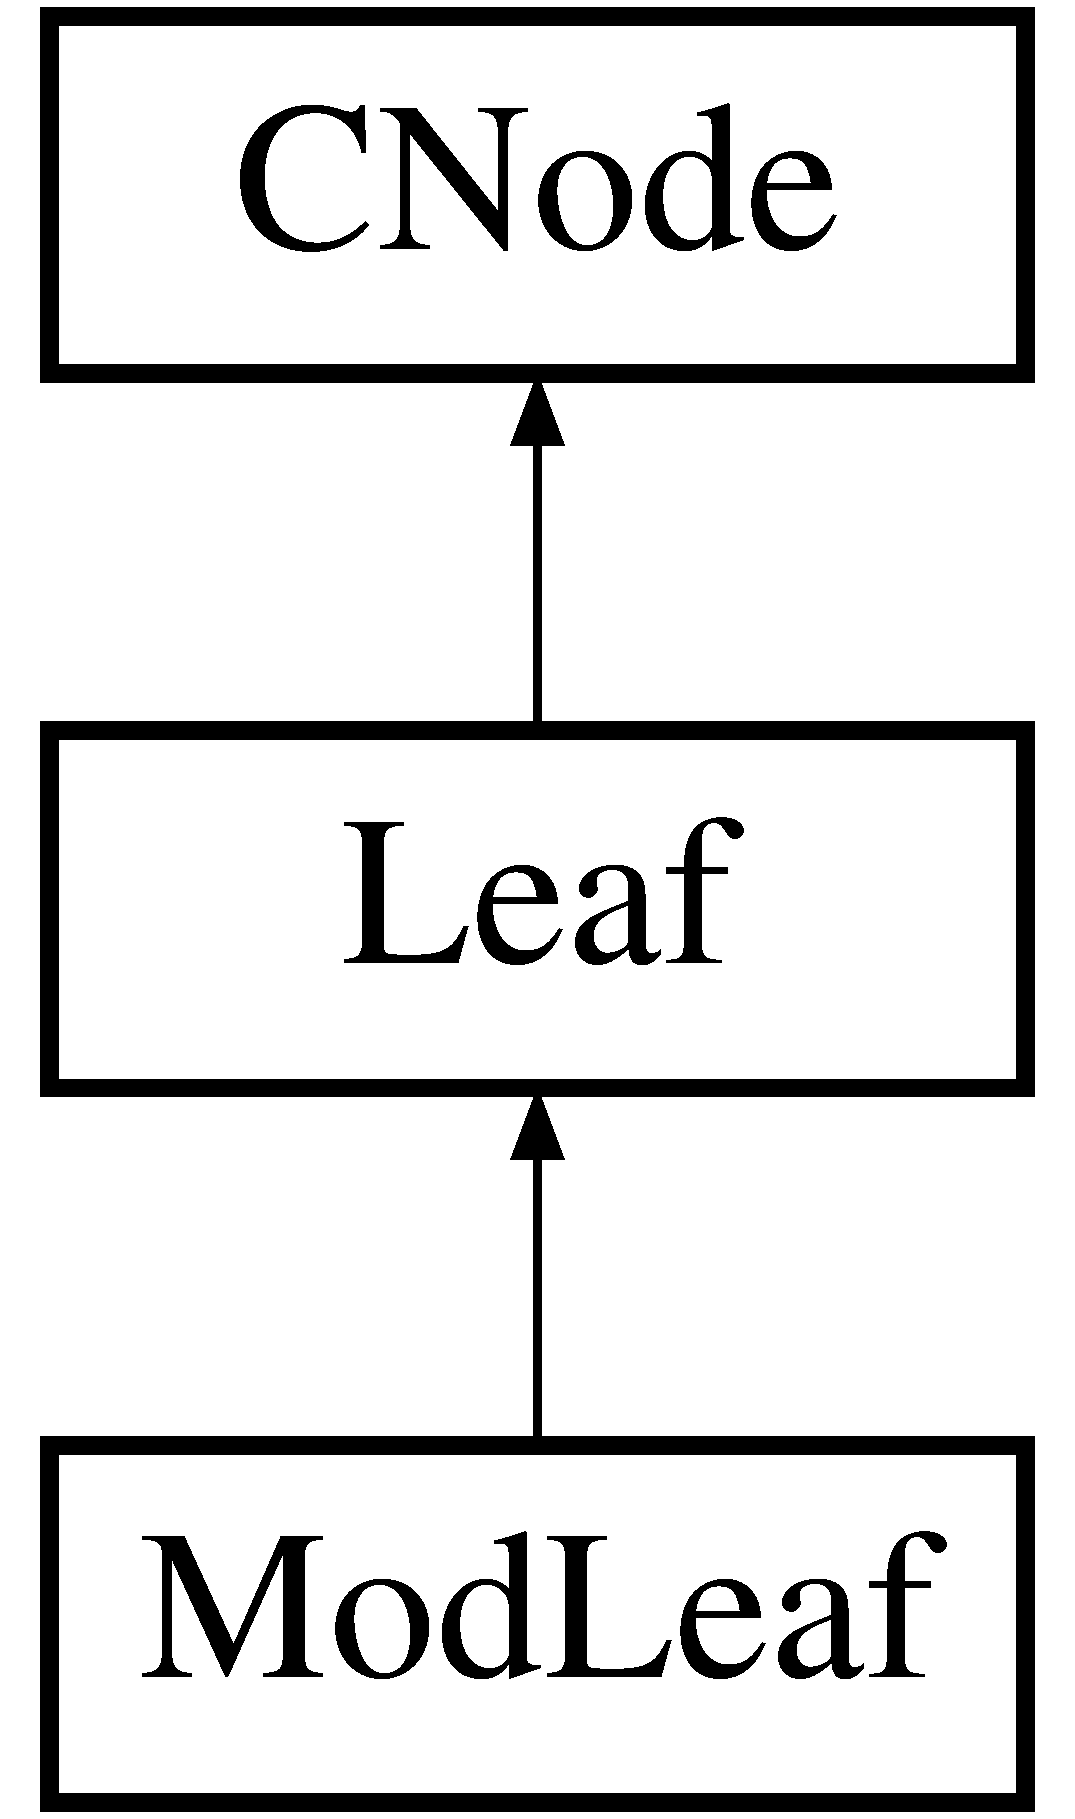
\includegraphics[height=3.000000cm]{classModLeaf}
\end{center}
\end{figure}
\subsection*{\-Public \-Member \-Functions}
\begin{DoxyCompactItemize}
\item 
\hypertarget{classModLeaf_a5828eba46e2ec9de959db626779f3337}{\hyperlink{classTerm}{\-Term} $\ast$ {\bfseries get\-\_\-term} ()}\label{classModLeaf_a5828eba46e2ec9de959db626779f3337}

\item 
\hypertarget{classModLeaf_ae41cfdbd628e3ef2055527d7a9a332f4}{long int {\bfseries get\-\_\-mod\-\_\-constant} ()}\label{classModLeaf_ae41cfdbd628e3ef2055527d7a9a332f4}

\item 
\hypertarget{classModLeaf_a92f1a0251e0c32a27387ac2b9599a2c9}{void {\bfseries to\-\_\-ilp} (set$<$ \hyperlink{classILPLeaf}{\-I\-L\-P\-Leaf} $\ast$ $>$ \&ilp\-\_\-leaves, bool pos, int temp\-\_\-id)}\label{classModLeaf_a92f1a0251e0c32a27387ac2b9599a2c9}

\item 
\hypertarget{classModLeaf_a9edb8af1b7ff81da17b099391a435b26}{virtual bool {\bfseries operator==} (const \hyperlink{classCNode}{\-C\-Node} \&other)}\label{classModLeaf_a9edb8af1b7ff81da17b099391a435b26}

\item 
\hypertarget{classModLeaf_a415e2fed13664bf2b850bb76d068c843}{virtual \hyperlink{classCNode}{\-C\-Node} $\ast$ {\bfseries substitute} (map$<$ \hyperlink{classTerm}{\-Term} $\ast$, \hyperlink{classTerm}{\-Term} $\ast$ $>$ \&subs)}\label{classModLeaf_a415e2fed13664bf2b850bb76d068c843}

\item 
\hypertarget{classModLeaf_aea07a828e00ab8f36326e3bcc16eb72f}{virtual string {\bfseries to\-\_\-string} ()}\label{classModLeaf_aea07a828e00ab8f36326e3bcc16eb72f}

\item 
\hypertarget{classModLeaf_a313b14e933bbf213c3ff378e82919918}{\hyperlink{classVariableTerm}{\-Variable\-Term} $\ast$ {\bfseries get\-\_\-ilp\-\_\-temp} (int temp\-\_\-id)}\label{classModLeaf_a313b14e933bbf213c3ff378e82919918}

\item 
\hypertarget{classModLeaf_a4be49a149d49b10182179a5ca58cd417}{pair$<$ \hyperlink{classVariableTerm}{\-Variable\-Term} \*
$\ast$, \hyperlink{classVariableTerm}{\-Variable\-Term} $\ast$ $>$ {\bfseries get\-\_\-ilp\-\_\-temps} (int temp\-\_\-id)}\label{classModLeaf_a4be49a149d49b10182179a5ca58cd417}

\end{DoxyCompactItemize}
\subsection*{\-Static \-Public \-Member \-Functions}
\begin{DoxyCompactItemize}
\item 
\hypertarget{classModLeaf_a9687353c013510b29fef1b126a9d0185}{static \hyperlink{classCNode}{\-C\-Node} $\ast$ {\bfseries make} (\hyperlink{classTerm}{\-Term} $\ast$t, long int k, \hyperlink{classTerm}{\-Term} $\ast$r)}\label{classModLeaf_a9687353c013510b29fef1b126a9d0185}

\item 
\hypertarget{classModLeaf_a91e39eacd261b1f463a45081dede7d41}{static \hyperlink{classCNode}{\-C\-Node} $\ast$ {\bfseries make} (\hyperlink{classTerm}{\-Term} $\ast$t, long int k, long int r)}\label{classModLeaf_a91e39eacd261b1f463a45081dede7d41}

\item 
\hypertarget{classModLeaf_abf7788797fec8d1b195f046e4ffa0ee0}{static \hyperlink{classCNode}{\-C\-Node} $\ast$ {\bfseries make} (\hyperlink{classTerm}{\-Term} $\ast$t, long int k)}\label{classModLeaf_abf7788797fec8d1b195f046e4ffa0ee0}

\end{DoxyCompactItemize}
\subsection*{\-Protected \-Member \-Functions}
\begin{DoxyCompactItemize}
\item 
\hypertarget{classModLeaf_a463bf691a2eed88a4993794f1a5a7564}{{\bfseries \-Mod\-Leaf} (\hyperlink{classTerm}{\-Term} $\ast$t, long int k)}\label{classModLeaf_a463bf691a2eed88a4993794f1a5a7564}

\end{DoxyCompactItemize}
\subsection*{\-Friends}
\begin{DoxyCompactItemize}
\item 
\hypertarget{classModLeaf_ac98d07dd8f7b70e16ccb9a01abf56b9c}{class {\bfseries boost\-::serialization\-::access}}\label{classModLeaf_ac98d07dd8f7b70e16ccb9a01abf56b9c}

\end{DoxyCompactItemize}


\-The documentation for this class was generated from the following files\-:\begin{DoxyCompactItemize}
\item 
cnode/\-Mod\-Leaf.\-h\item 
cnode/\-Mod\-Leaf.\-cpp\end{DoxyCompactItemize}

\hypertarget{classMSAFinder}{\section{\-M\-S\-A\-Finder \-Class \-Reference}
\label{classMSAFinder}\index{\-M\-S\-A\-Finder@{\-M\-S\-A\-Finder}}
}
\subsection*{\-Public \-Member \-Functions}
\begin{DoxyCompactItemize}
\item 
\hypertarget{classMSAFinder_a2a25978d31ed79fb09f7a94cad9d181d}{{\bfseries \-M\-S\-A\-Finder} (\hyperlink{classCNode}{\-C\-Node} $\ast$node, map$<$ \hyperlink{classVariableTerm}{\-Variable\-Term} $\ast$, int $>$ \&costs)}\label{classMSAFinder_a2a25978d31ed79fb09f7a94cad9d181d}

\item 
\hypertarget{classMSAFinder_ab32e9c297724f65fdf6b2b6b7c07473f}{{\bfseries \-M\-S\-A\-Finder} (\hyperlink{classCNode}{\-C\-Node} $\ast$c, set$<$ \hyperlink{classCNode}{\-C\-Node} $\ast$ $>$ \&background, map$<$ \hyperlink{classVariableTerm}{\-Variable\-Term} $\ast$, int $>$ \&costs)}\label{classMSAFinder_ab32e9c297724f65fdf6b2b6b7c07473f}

\item 
\hypertarget{classMSAFinder_a4ac67540b4837447192a3edee8f5bb82}{const set$<$ \hyperlink{classVariableTerm}{\-Variable\-Term} $\ast$ $>$ \& {\bfseries get\-\_\-vars\-\_\-in\-\_\-msa} ()}\label{classMSAFinder_a4ac67540b4837447192a3edee8f5bb82}

\item 
\hypertarget{classMSAFinder_a43f453ab387cbed3cda1e12bea45b896}{int {\bfseries get\-\_\-cost} ()}\label{classMSAFinder_a43f453ab387cbed3cda1e12bea45b896}

\item 
\hypertarget{classMSAFinder_a49f093494327a0fd187fe21df8bb9345}{string {\bfseries get\-\_\-stats} ()}\label{classMSAFinder_a49f093494327a0fd187fe21df8bb9345}

\item 
\hypertarget{classMSAFinder_ab79f4be9438081d31b0042a58c5dfb31}{string {\bfseries res\-\_\-to\-\_\-string} ()}\label{classMSAFinder_ab79f4be9438081d31b0042a58c5dfb31}

\end{DoxyCompactItemize}
\subsection*{\-Public \-Attributes}
\begin{DoxyCompactItemize}
\item 
\hypertarget{classMSAFinder_a4f3a5aabfec12ac2c746d73bff086fad}{\hyperlink{classCNode}{\-C\-Node} $\ast$ {\bfseries node}}\label{classMSAFinder_a4f3a5aabfec12ac2c746d73bff086fad}

\item 
\hypertarget{classMSAFinder_aec0b42aac87eec1e9ab9ea609dc33a73}{map$<$ \hyperlink{classVariableTerm}{\-Variable\-Term} $\ast$, int $>$ \& {\bfseries costs}}\label{classMSAFinder_aec0b42aac87eec1e9ab9ea609dc33a73}

\item 
\hypertarget{classMSAFinder_a85e3b87a536e1ade8780db1ffa196ab6}{int {\bfseries min\-\_\-estimate}}\label{classMSAFinder_a85e3b87a536e1ade8780db1ffa196ab6}

\item 
\hypertarget{classMSAFinder_aef83482fbb0c7eae2885683b6004cc8e}{set$<$ \hyperlink{classVariableTerm}{\-Variable\-Term} $\ast$ $>$ {\bfseries msa}}\label{classMSAFinder_aef83482fbb0c7eae2885683b6004cc8e}

\item 
\hypertarget{classMSAFinder_af202e914a39d5288888d69d43f42cc41}{map$<$ \hyperlink{classVariableTerm}{\-Variable\-Term} $\ast$, \hyperlink{classTerm}{\-Term} $\ast$ $>$ {\bfseries var\-\_\-to\-\_\-fun\-\_\-map}}\label{classMSAFinder_af202e914a39d5288888d69d43f42cc41}

\item 
\hypertarget{classMSAFinder_a3f487ac299a4a57c44fbffc94ffeeb8e}{map$<$ \hyperlink{classTerm}{\-Term} $\ast$, set$<$ set$<$ \hyperlink{classTerm}{\-Term} $\ast$ $>$ $>$ $>$ {\bfseries dependencies}}\label{classMSAFinder_a3f487ac299a4a57c44fbffc94ffeeb8e}

\item 
\hypertarget{classMSAFinder_a342d81bbf463c5924cd1d673447b9b16}{int {\bfseries mpi\-\_\-estimate}}\label{classMSAFinder_a342d81bbf463c5924cd1d673447b9b16}

\item 
\hypertarget{classMSAFinder_a419dd9b3e2bdef459a813a1b3c85d286}{int {\bfseries fun\-\_\-counter}}\label{classMSAFinder_a419dd9b3e2bdef459a813a1b3c85d286}

\item 
\hypertarget{classMSAFinder_a5e2ee66762738511ae6505d702d39f83}{int {\bfseries num\-\_\-e\-\_\-elims}}\label{classMSAFinder_a5e2ee66762738511ae6505d702d39f83}

\item 
\hypertarget{classMSAFinder_a9fc51cfb947318b263392a048cd759d0}{int {\bfseries e\-\_\-elim\-\_\-time}}\label{classMSAFinder_a9fc51cfb947318b263392a048cd759d0}

\item 
\hypertarget{classMSAFinder_af5d685140bc2bbca181b8d6e4c6a2987}{int {\bfseries num\-\_\-a\-\_\-elims}}\label{classMSAFinder_af5d685140bc2bbca181b8d6e4c6a2987}

\item 
\hypertarget{classMSAFinder_a14cb7b8e44dbabf194a515e832a4af94}{int {\bfseries a\-\_\-elim\-\_\-time}}\label{classMSAFinder_a14cb7b8e44dbabf194a515e832a4af94}

\item 
\hypertarget{classMSAFinder_a421e15cf6cce0a7c42542449df47e9b8}{int {\bfseries a\-\_\-approximate}}\label{classMSAFinder_a421e15cf6cce0a7c42542449df47e9b8}

\item 
\hypertarget{classMSAFinder_ad362b36bca3886acbed19bb5c0563cfa}{int {\bfseries a\-\_\-approximate\-\_\-time}}\label{classMSAFinder_ad362b36bca3886acbed19bb5c0563cfa}

\item 
\hypertarget{classMSAFinder_aaf66c483fd42f4efa4e8f9efab0ce726}{int {\bfseries num\-\_\-unsat\-\_\-universal}}\label{classMSAFinder_aaf66c483fd42f4efa4e8f9efab0ce726}

\item 
\hypertarget{classMSAFinder_ab2356dba9e517906627e119f3510d44b}{int {\bfseries num\-\_\-unsat\-\_\-approx\-\_\-universal}}\label{classMSAFinder_ab2356dba9e517906627e119f3510d44b}

\item 
\hypertarget{classMSAFinder_a7851b9b4684eaa4ee979c4009ea14956}{int {\bfseries dependence\-\_\-time}}\label{classMSAFinder_a7851b9b4684eaa4ee979c4009ea14956}

\item 
\hypertarget{classMSAFinder_ae801e8c605d4c6922ec49cbff47e88f3}{int {\bfseries num\-\_\-dep\-\_\-success}}\label{classMSAFinder_ae801e8c605d4c6922ec49cbff47e88f3}

\item 
\hypertarget{classMSAFinder_a4db5a809f0bb9b43881298c88abffe53}{int {\bfseries simplify\-\_\-time}}\label{classMSAFinder_a4db5a809f0bb9b43881298c88abffe53}

\item 
\hypertarget{classMSAFinder_a025777870f3a665e6d44f0ff605f7592}{int {\bfseries mpi\-\_\-time}}\label{classMSAFinder_a025777870f3a665e6d44f0ff605f7592}

\item 
\hypertarget{classMSAFinder_a1c83e8e87c58558da27167916c89abf4}{int {\bfseries prune1\-\_\-solve}}\label{classMSAFinder_a1c83e8e87c58558da27167916c89abf4}

\item 
\hypertarget{classMSAFinder_a169289fa1519ad78fbd4c2e112cfa844}{int {\bfseries prune2\-\_\-solve}}\label{classMSAFinder_a169289fa1519ad78fbd4c2e112cfa844}

\item 
\hypertarget{classMSAFinder_aed6453abcfd412a1013cb7cea46c501c}{int {\bfseries e\-\_\-only}}\label{classMSAFinder_aed6453abcfd412a1013cb7cea46c501c}

\item 
\hypertarget{classMSAFinder_a6558a1c7b4874e5ce07344dd440ebe97}{int {\bfseries a\-\_\-only}}\label{classMSAFinder_a6558a1c7b4874e5ce07344dd440ebe97}

\item 
\hypertarget{classMSAFinder_aef3c091db425df97637b9480e17aac55}{int {\bfseries total}}\label{classMSAFinder_aef3c091db425df97637b9480e17aac55}

\item 
\hypertarget{classMSAFinder_aa61506b9343333d49263a7780c71393d}{int {\bfseries cost\-\_\-pruned}}\label{classMSAFinder_aa61506b9343333d49263a7780c71393d}

\item 
\hypertarget{classMSAFinder_ac680e97f6d2e20bab5a4d7711727869d}{int {\bfseries max\-\_\-cost}}\label{classMSAFinder_ac680e97f6d2e20bab5a4d7711727869d}

\item 
\hypertarget{classMSAFinder_aaf89914b503c4b2f9390e2c02f05a667}{set$<$ \hyperlink{classTerm}{\-Term} $\ast$ $>$ {\bfseries vars\-\_\-in\-\_\-min\-\_\-pi}}\label{classMSAFinder_aaf89914b503c4b2f9390e2c02f05a667}

\end{DoxyCompactItemize}


\-The documentation for this class was generated from the following files\-:\begin{DoxyCompactItemize}
\item 
solver/\-M\-S\-A\-Finder.\-h\item 
solver/\-M\-S\-A\-Finder.\-cpp\end{DoxyCompactItemize}

\hypertarget{structnode__eq}{\section{node\-\_\-eq \-Struct \-Reference}
\label{structnode__eq}\index{node\-\_\-eq@{node\-\_\-eq}}
}
\subsection*{\-Public \-Member \-Functions}
\begin{DoxyCompactItemize}
\item 
\hypertarget{structnode__eq_a96000e1dd0e3f726c05c4f98f98cd2b7}{bool {\bfseries operator()} (const \hyperlink{classCNode}{\-C\-Node} $\ast$l1, const \hyperlink{classCNode}{\-C\-Node} $\ast$l2) const }\label{structnode__eq_a96000e1dd0e3f726c05c4f98f98cd2b7}

\end{DoxyCompactItemize}


\-The documentation for this struct was generated from the following files\-:\begin{DoxyCompactItemize}
\item 
cnode/\-C\-Node.\-h\item 
cnode/\-C\-Node.\-cpp\end{DoxyCompactItemize}

\hypertarget{classNormalForm}{\section{\-Normal\-Form \-Class \-Reference}
\label{classNormalForm}\index{\-Normal\-Form@{\-Normal\-Form}}
}
\subsection*{\-Public \-Member \-Functions}
\begin{DoxyCompactItemize}
\item 
\hypertarget{classNormalForm_aec09071c299bcae2ac856aa546e08a20}{{\bfseries \-Normal\-Form} (\hyperlink{classCNode}{\-C\-Node} $\ast$n, bool is\-\_\-dnf)}\label{classNormalForm_aec09071c299bcae2ac856aa546e08a20}

\item 
\hypertarget{classNormalForm_acc0a30a393e9fb0bb300151e421908ad}{set$<$ \hyperlink{classClause}{\-Clause} $\ast$ $>$ $\ast$ {\bfseries get\-\_\-clauses} ()}\label{classNormalForm_acc0a30a393e9fb0bb300151e421908ad}

\item 
\hypertarget{classNormalForm_af7a02c573646d49b0d9b237f2d816706}{string {\bfseries to\-\_\-string} (\hyperlink{classVarMap}{\-Var\-Map} \&vm)}\label{classNormalForm_af7a02c573646d49b0d9b237f2d816706}

\item 
\hypertarget{classNormalForm_a1aada9f719a46070fd4dbc3ed7c21875}{\hyperlink{classCNode}{\-C\-Node} $\ast$ {\bfseries get\-\_\-constraint} ()}\label{classNormalForm_a1aada9f719a46070fd4dbc3ed7c21875}

\end{DoxyCompactItemize}
\subsection*{\-Static \-Public \-Member \-Functions}
\begin{DoxyCompactItemize}
\item 
\hypertarget{classNormalForm_ac71bf2b54a1fa6959bf8dde54a295996}{static \hyperlink{classCNode}{\-C\-Node} $\ast$ {\bfseries get\-\_\-constraint\-\_\-from\-\_\-clause} (\hyperlink{classClause}{\-Clause} $\ast$c, bool use\-\_\-and)}\label{classNormalForm_ac71bf2b54a1fa6959bf8dde54a295996}

\end{DoxyCompactItemize}


\-The documentation for this class was generated from the following files\-:\begin{DoxyCompactItemize}
\item 
solver/\-Normal\-Form.\-h\item 
solver/\-Normal\-Form.\-cpp\end{DoxyCompactItemize}

\hypertarget{classOptimizer}{\section{\-Optimizer \-Class \-Reference}
\label{classOptimizer}\index{\-Optimizer@{\-Optimizer}}
}
\subsection*{\-Public \-Member \-Functions}
\begin{DoxyCompactItemize}
\item 
\hypertarget{classOptimizer_a35ee40c7e5bd5735eb8fc7ea121961a4}{{\bfseries \-Optimizer} (\hyperlink{classCNode}{\-C\-Node} $\ast$c, \hyperlink{classTerm}{\-Term} $\ast$cost\-\_\-fn, bool min, long int bound, int num\-\_\-iterations=-\/1)}\label{classOptimizer_a35ee40c7e5bd5735eb8fc7ea121961a4}

\item 
\hypertarget{classOptimizer_a6125345c0b713278e989ffe2918839d1}{long int {\bfseries get\-\_\-optimal\-\_\-cost} ()}\label{classOptimizer_a6125345c0b713278e989ffe2918839d1}

\item 
\hypertarget{classOptimizer_aa945fcb4b4e2614d82f9d9e1eb64d759}{const map$<$ \hyperlink{classTerm}{\-Term} $\ast$, \hyperlink{classSatValue}{\-Sat\-Value} $>$ \& {\bfseries get\-\_\-assignment} ()}\label{classOptimizer_aa945fcb4b4e2614d82f9d9e1eb64d759}

\item 
\hypertarget{classOptimizer_a986f4b83737d16a76be1943200f750f1}{string {\bfseries get\-\_\-stats} ()}\label{classOptimizer_a986f4b83737d16a76be1943200f750f1}

\end{DoxyCompactItemize}


\-The documentation for this class was generated from the following files\-:\begin{DoxyCompactItemize}
\item 
solver/\-Optimizer.\-h\item 
solver/\-Optimizer.\-cpp\end{DoxyCompactItemize}

\hypertarget{classOptionColumns}{\section{\-Option\-Columns \-Class \-Reference}
\label{classOptionColumns}\index{\-Option\-Columns@{\-Option\-Columns}}
}
\subsection*{\-Public \-Attributes}
\begin{DoxyCompactItemize}
\item 
\hypertarget{classOptionColumns_a95f0d7286b169d66b107a5bec36e2c7a}{\-Gtk\-::\-Tree\-Model\-Column$<$ string $>$ {\bfseries col\-\_\-id}}\label{classOptionColumns_a95f0d7286b169d66b107a5bec36e2c7a}

\end{DoxyCompactItemize}


\-The documentation for this class was generated from the following file\-:\begin{DoxyCompactItemize}
\item 
ui/src/solver-\/ui.\-cpp\end{DoxyCompactItemize}

\hypertarget{unionparse__res__union}{\section{parse\-\_\-res\-\_\-union \-Union \-Reference}
\label{unionparse__res__union}\index{parse\-\_\-res\-\_\-union@{parse\-\_\-res\-\_\-union}}
}
\subsection*{\-Public \-Attributes}
\begin{DoxyCompactItemize}
\item 
\hypertarget{unionparse__res__union_aae9e9d66a34463b4a5f08724c9cb6f07}{\hyperlink{classCNode}{\-C\-Node} $\ast$ {\bfseries c}}\label{unionparse__res__union_aae9e9d66a34463b4a5f08724c9cb6f07}

\item 
\hypertarget{unionparse__res__union_a47eeb8862a489e7a539fea78f7315638}{\hyperlink{classTerm}{\-Term} $\ast$ {\bfseries t}}\label{unionparse__res__union_a47eeb8862a489e7a539fea78f7315638}

\item 
\hypertarget{unionparse__res__union_ab8d40a5315ced30ab697807bbf9e510d}{string $\ast$ {\bfseries s}}\label{unionparse__res__union_ab8d40a5315ced30ab697807bbf9e510d}

\end{DoxyCompactItemize}


\-The documentation for this union was generated from the following files\-:\begin{DoxyCompactItemize}
\item 
parser/mistral-\/parser-\/defs.\-h\item 
smtparser/smt-\/parser-\/defs.\-h\end{DoxyCompactItemize}

\hypertarget{structparse__result}{\section{parse\-\_\-result \-Struct \-Reference}
\label{structparse__result}\index{parse\-\_\-result@{parse\-\_\-result}}
}
\subsection*{\-Public \-Attributes}
\begin{DoxyCompactItemize}
\item 
\hypertarget{structparse__result_aed1a4ff6458f5ec2733581b60c350588}{\-P\-A\-R\-S\-E\-\_\-\-K\-I\-N\-D {\bfseries kind}}\label{structparse__result_aed1a4ff6458f5ec2733581b60c350588}

\item 
\hypertarget{structparse__result_a906c64fe973951f0b44e3a38017ff579}{\hyperlink{unionparse__res__union}{parse\-\_\-res\-\_\-union} {\bfseries res}}\label{structparse__result_a906c64fe973951f0b44e3a38017ff579}

\end{DoxyCompactItemize}


\-The documentation for this struct was generated from the following files\-:\begin{DoxyCompactItemize}
\item 
parser/mistral-\/parser-\/defs.\-h\item 
smtparser/smt-\/parser-\/defs.\-h\end{DoxyCompactItemize}

\hypertarget{classQuantifiedLeaf}{\section{\-Quantified\-Leaf \-Class \-Reference}
\label{classQuantifiedLeaf}\index{\-Quantified\-Leaf@{\-Quantified\-Leaf}}
}
\-Inheritance diagram for \-Quantified\-Leaf\-:\begin{figure}[H]
\begin{center}
\leavevmode
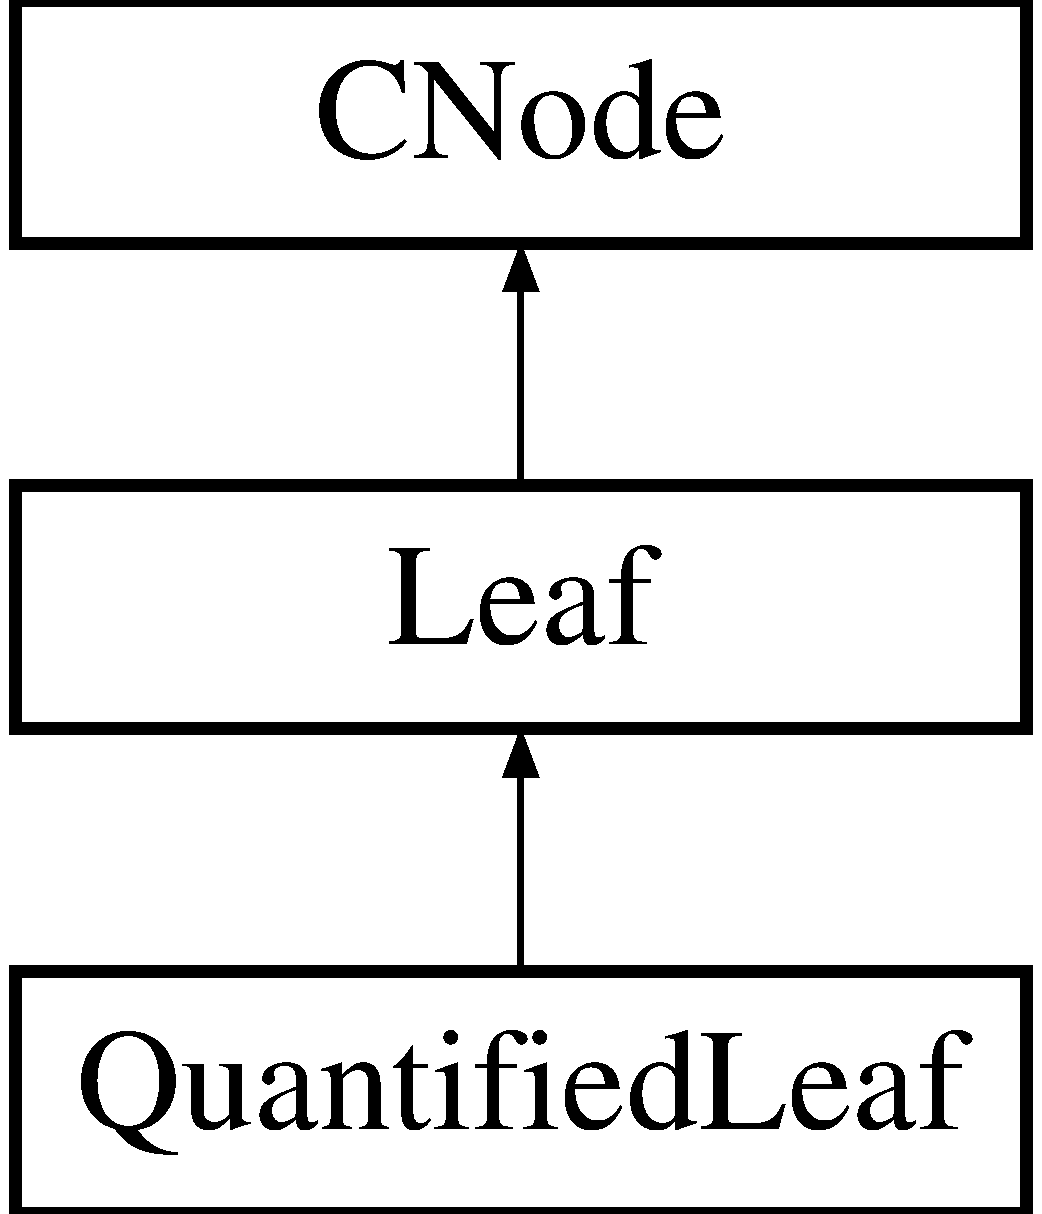
\includegraphics[height=3.000000cm]{classQuantifiedLeaf}
\end{center}
\end{figure}
\subsection*{\-Public \-Member \-Functions}
\begin{DoxyCompactItemize}
\item 
\hypertarget{classQuantifiedLeaf_a10affbbc61d18f065e230d4848ef2e55}{set$<$ int $>$ \& {\bfseries get\-\_\-quantified\-\_\-vars} ()}\label{classQuantifiedLeaf_a10affbbc61d18f065e230d4848ef2e55}

\item 
\hypertarget{classQuantifiedLeaf_a6aef6c1fa3451ed60857d60c77dfd94a}{\hyperlink{classCNode}{\-C\-Node} $\ast$ {\bfseries get\-\_\-index\-\_\-guard} ()}\label{classQuantifiedLeaf_a6aef6c1fa3451ed60857d60c77dfd94a}

\item 
\hypertarget{classQuantifiedLeaf_aa8b0d5eab65f9a0b2957e9eab5af6dfd}{\hyperlink{classCNode}{\-C\-Node} $\ast$ {\bfseries get\-\_\-value\-\_\-guard} ()}\label{classQuantifiedLeaf_aa8b0d5eab65f9a0b2957e9eab5af6dfd}

\item 
\hypertarget{classQuantifiedLeaf_ab46b71c4cb35fbf9ab3d31ca915423b8}{virtual bool {\bfseries operator==} (const \hyperlink{classCNode}{\-C\-Node} \&other)}\label{classQuantifiedLeaf_ab46b71c4cb35fbf9ab3d31ca915423b8}

\item 
\hypertarget{classQuantifiedLeaf_aec92f796105418177b33b169ed32c4f0}{virtual string {\bfseries to\-\_\-string} ()}\label{classQuantifiedLeaf_aec92f796105418177b33b169ed32c4f0}

\item 
\hypertarget{classQuantifiedLeaf_a56f45ca0ee111c4f8fee1c511fba1add}{virtual \hyperlink{classCNode}{\-C\-Node} $\ast$ {\bfseries substitute} (map$<$ \hyperlink{classTerm}{\-Term} $\ast$, \hyperlink{classTerm}{\-Term} $\ast$ $>$ \&subs)}\label{classQuantifiedLeaf_a56f45ca0ee111c4f8fee1c511fba1add}

\end{DoxyCompactItemize}
\subsection*{\-Static \-Public \-Member \-Functions}
\begin{DoxyCompactItemize}
\item 
\hypertarget{classQuantifiedLeaf_a7161b27997f0d66fbb4ab491c777619e}{static \hyperlink{classCNode}{\-C\-Node} $\ast$ {\bfseries make} (set$<$ int $>$ \&q\-\_\-vars, \hyperlink{classCNode}{\-C\-Node} $\ast$index\-\_\-guard, \hyperlink{classCNode}{\-C\-Node} $\ast$value\-\_\-guard)}\label{classQuantifiedLeaf_a7161b27997f0d66fbb4ab491c777619e}

\end{DoxyCompactItemize}
\subsection*{\-Protected \-Member \-Functions}
\begin{DoxyCompactItemize}
\item 
\hypertarget{classQuantifiedLeaf_a577808987e7b5646592b282fb3f24386}{{\bfseries \-Quantified\-Leaf} (set$<$ int $>$ \&q\-\_\-vars, \hyperlink{classCNode}{\-C\-Node} $\ast$index\-\_\-guard, \hyperlink{classCNode}{\-C\-Node} $\ast$value\-\_\-guard)}\label{classQuantifiedLeaf_a577808987e7b5646592b282fb3f24386}

\end{DoxyCompactItemize}
\subsection*{\-Friends}
\begin{DoxyCompactItemize}
\item 
\hypertarget{classQuantifiedLeaf_ac98d07dd8f7b70e16ccb9a01abf56b9c}{class {\bfseries boost\-::serialization\-::access}}\label{classQuantifiedLeaf_ac98d07dd8f7b70e16ccb9a01abf56b9c}

\end{DoxyCompactItemize}


\-The documentation for this class was generated from the following files\-:\begin{DoxyCompactItemize}
\item 
cnode/\-Quantified\-Leaf.\-h\item 
cnode/\-Quantified\-Leaf.\-cpp\end{DoxyCompactItemize}

\hypertarget{classQueryComparator}{\section{\-Query\-Comparator \-Class \-Reference}
\label{classQueryComparator}\index{\-Query\-Comparator@{\-Query\-Comparator}}
}
\subsection*{\-Public \-Member \-Functions}
\begin{DoxyCompactItemize}
\item 
\hypertarget{classQueryComparator_a07bd1c21936f883c8f1870b5340c1f93}{bool {\bfseries operator()} (const \hyperlink{classILPQuery}{\-I\-L\-P\-Query} $\ast$const \&\-\_\-q1, const \hyperlink{classILPQuery}{\-I\-L\-P\-Query} $\ast$const \&\-\_\-q2) const }\label{classQueryComparator_a07bd1c21936f883c8f1870b5340c1f93}

\end{DoxyCompactItemize}


\-The documentation for this class was generated from the following file\-:\begin{DoxyCompactItemize}
\item 
solver/\-Interaction\-Manager.\-cpp\end{DoxyCompactItemize}

\hypertarget{classQueue}{\section{\-Queue$<$ \-T $>$ \-Class \-Template \-Reference}
\label{classQueue}\index{\-Queue$<$ T $>$@{\-Queue$<$ T $>$}}
}
\subsection*{\-Public \-Member \-Functions}
\begin{DoxyCompactItemize}
\item 
\hypertarget{classQueue_a1d313317eb2c8a1b41e2bf85f33f121b}{void {\bfseries insert} (\-T x)}\label{classQueue_a1d313317eb2c8a1b41e2bf85f33f121b}

\item 
\hypertarget{classQueue_a12e913387d6d082d473d7e8d919943d9}{\-T {\bfseries peek} () const }\label{classQueue_a12e913387d6d082d473d7e8d919943d9}

\item 
\hypertarget{classQueue_a02ea784625fe33b5793d00c3b02b4878}{void {\bfseries pop} ()}\label{classQueue_a02ea784625fe33b5793d00c3b02b4878}

\item 
\hypertarget{classQueue_a24d60f28f7ea91dfe71804f6c9b00805}{void {\bfseries clear} (bool dealloc=false)}\label{classQueue_a24d60f28f7ea91dfe71804f6c9b00805}

\item 
\hypertarget{classQueue_a05135474a17e883dc4fe2b0560032459}{int {\bfseries size} (void)}\label{classQueue_a05135474a17e883dc4fe2b0560032459}

\item 
\hypertarget{classQueue_acaefcc6efcb518de379b65c27befbc81}{const \-T \& {\bfseries operator\mbox{[}$\,$\mbox{]}} (int index) const }\label{classQueue_acaefcc6efcb518de379b65c27befbc81}

\end{DoxyCompactItemize}
\subsubsection*{template$<$class T$>$ class Queue$<$ T $>$}



\-The documentation for this class was generated from the following file\-:\begin{DoxyCompactItemize}
\item 
sat-\/solver/\-Queue.\-h\end{DoxyCompactItemize}

\hypertarget{structqvar}{\section{qvar \-Struct \-Reference}
\label{structqvar}\index{qvar@{qvar}}
}
\subsection*{\-Public \-Member \-Functions}
\begin{DoxyCompactItemize}
\item 
\hypertarget{structqvar_aca3d02f8800c57b7e4e474305bb70b03}{bool {\bfseries operator$<$} (const \hyperlink{structqvar}{qvar} \&other) const }\label{structqvar_aca3d02f8800c57b7e4e474305bb70b03}

\end{DoxyCompactItemize}
\subsection*{\-Public \-Attributes}
\begin{DoxyCompactItemize}
\item 
\hypertarget{structqvar_a8e0639b72797b150e0c2c39b6a76c118}{long int {\bfseries id}}\label{structqvar_a8e0639b72797b150e0c2c39b6a76c118}

\item 
\hypertarget{structqvar_a20f7da0b88ce7f066a2d05ac995fac9c}{int {\bfseries var\-\_\-id}}\label{structqvar_a20f7da0b88ce7f066a2d05ac995fac9c}

\end{DoxyCompactItemize}


\-The documentation for this struct was generated from the following file\-:\begin{DoxyCompactItemize}
\item 
solver/\-Universal\-Instantiator.\-h\end{DoxyCompactItemize}

\hypertarget{classRegressionModelColumns}{\section{\-Regression\-Model\-Columns \-Class \-Reference}
\label{classRegressionModelColumns}\index{\-Regression\-Model\-Columns@{\-Regression\-Model\-Columns}}
}
\subsection*{\-Public \-Attributes}
\begin{DoxyCompactItemize}
\item 
\hypertarget{classRegressionModelColumns_a234da2cc7ccd81da07989976a170041b}{\-Gtk\-::\-Tree\-Model\-Column$<$ string $>$ {\bfseries col\-\_\-id}}\label{classRegressionModelColumns_a234da2cc7ccd81da07989976a170041b}

\item 
\hypertarget{classRegressionModelColumns_a2047c46be9766377c95bf9440da98bd9}{\-Gtk\-::\-Tree\-Model\-Column$<$ string $>$ {\bfseries col\-\_\-status}}\label{classRegressionModelColumns_a2047c46be9766377c95bf9440da98bd9}

\item 
\hypertarget{classRegressionModelColumns_afbe7653effc4c5a879ec6cbd659d615e}{\-Gtk\-::\-Tree\-Model\-Column$<$ string $>$ {\bfseries col\-\_\-res}}\label{classRegressionModelColumns_afbe7653effc4c5a879ec6cbd659d615e}

\item 
\hypertarget{classRegressionModelColumns_a9d455f88270a82789612e1be36a45317}{\-Gtk\-::\-Tree\-Model\-Column$<$ string $>$ {\bfseries col\-\_\-time}}\label{classRegressionModelColumns_a9d455f88270a82789612e1be36a45317}

\item 
\hypertarget{classRegressionModelColumns_aa7175ca9177af7d051db93a52ce7870d}{\-Gtk\-::\-Tree\-Model\-Column$<$ string $>$ {\bfseries col\-\_\-size}}\label{classRegressionModelColumns_aa7175ca9177af7d051db93a52ce7870d}

\end{DoxyCompactItemize}


\-The documentation for this class was generated from the following file\-:\begin{DoxyCompactItemize}
\item 
ui/src/solver-\/ui.\-cpp\end{DoxyCompactItemize}

\hypertarget{classsail_1_1Variable}{\section{sail\-:\-:\-Variable \-Class \-Reference}
\label{classsail_1_1Variable}\index{sail\-::\-Variable@{sail\-::\-Variable}}
}


\-The documentation for this class was generated from the following file\-:\begin{DoxyCompactItemize}
\item 
ui/src/solver-\/ui.\-cpp\end{DoxyCompactItemize}

\hypertarget{classSatValue}{\section{\-Sat\-Value \-Class \-Reference}
\label{classSatValue}\index{\-Sat\-Value@{\-Sat\-Value}}
}
\subsection*{\-Public \-Member \-Functions}
\begin{DoxyCompactItemize}
\item 
\hypertarget{classSatValue_a51713b4832cc812f019dcfa00aaecc66}{string {\bfseries to\-\_\-string} ()}\label{classSatValue_a51713b4832cc812f019dcfa00aaecc66}

\end{DoxyCompactItemize}
\subsection*{\-Public \-Attributes}
\begin{DoxyCompactItemize}
\item 
\hypertarget{classSatValue_a19af7b15b65ae5ee0ab8669571d4fdd3}{bool {\bfseries integer}}\label{classSatValue_a19af7b15b65ae5ee0ab8669571d4fdd3}

\item 
\hypertarget{classSatValue_a5058f4386247e43eceb43f936fd32c88}{\hyperlink{classbignum}{bignum} {\bfseries value}}\label{classSatValue_a5058f4386247e43eceb43f936fd32c88}

\end{DoxyCompactItemize}


\-The documentation for this class was generated from the following files\-:\begin{DoxyCompactItemize}
\item 
solver/\-Sat\-Value.\-h\item 
solver/\-Sat\-Value.\-cpp\end{DoxyCompactItemize}

\hypertarget{classScopeTable}{\section{\-Scope\-Table \-Class \-Reference}
\label{classScopeTable}\index{\-Scope\-Table@{\-Scope\-Table}}
}
\subsection*{\-Public \-Member \-Functions}
\begin{DoxyCompactItemize}
\item 
\hypertarget{classScopeTable_a17b3cdf7da3172bd41bece4728ca85a6}{void {\bfseries push} ()}\label{classScopeTable_a17b3cdf7da3172bd41bece4728ca85a6}

\item 
\hypertarget{classScopeTable_aa45f000b7ee2e70d103614942df9e0e4}{void {\bfseries pop} ()}\label{classScopeTable_aa45f000b7ee2e70d103614942df9e0e4}

\item 
\hypertarget{classScopeTable_a3e4786d324e44f4716fc9b45827a9a7e}{void {\bfseries put} (const string \&name, \hyperlink{classTerm}{\-Term} $\ast$t)}\label{classScopeTable_a3e4786d324e44f4716fc9b45827a9a7e}

\item 
\hypertarget{classScopeTable_a597f78e8f195ffefabfbe0e7b258e565}{\hyperlink{classTerm}{\-Term} $\ast$ {\bfseries get} (const string \&name)}\label{classScopeTable_a597f78e8f195ffefabfbe0e7b258e565}

\end{DoxyCompactItemize}


\-The documentation for this class was generated from the following file\-:\begin{DoxyCompactItemize}
\item 
smtparser/smt-\/parser-\/defs.\-h\end{DoxyCompactItemize}

\hypertarget{classSimplifier}{\section{\-Simplifier \-Class \-Reference}
\label{classSimplifier}\index{\-Simplifier@{\-Simplifier}}
}
\subsection*{\-Public \-Member \-Functions}
\begin{DoxyCompactItemize}
\item 
\hypertarget{classSimplifier_ac167c99291fc8a823d20c0db8cda6da5}{{\bfseries \-Simplifier} (\hyperlink{classCNode}{\-C\-Node} $\ast$node, \hyperlink{classCNode}{\-C\-Node} $\ast$background)}\label{classSimplifier_ac167c99291fc8a823d20c0db8cda6da5}

\item 
\hypertarget{classSimplifier_ad4e03d8d662ec9f6a1f6c1f05c726d5c}{{\bfseries \-Simplifier} (\hyperlink{classCNode}{\-C\-Node} $\ast$node, \hyperlink{classDPLLSolver}{\-D\-P\-L\-L\-Solver} $\ast$dpll\-\_\-solver, bool switch\-\_\-to\-\_\-boolean)}\label{classSimplifier_ad4e03d8d662ec9f6a1f6c1f05c726d5c}

\item 
\hypertarget{classSimplifier_ab84e47ceab782bb416a5da55ce807607}{\hyperlink{classCNode}{\-C\-Node} $\ast$ {\bfseries get\-\_\-simplification} ()}\label{classSimplifier_ab84e47ceab782bb416a5da55ce807607}

\end{DoxyCompactItemize}


\-The documentation for this class was generated from the following files\-:\begin{DoxyCompactItemize}
\item 
solver/\-Simplifier.\-h\item 
solver/\-Simplifier.\-cpp\end{DoxyCompactItemize}

\hypertarget{classSkeletonSolver}{\section{\-Skeleton\-Solver \-Class \-Reference}
\label{classSkeletonSolver}\index{\-Skeleton\-Solver@{\-Skeleton\-Solver}}
}
\subsection*{\-Public \-Member \-Functions}
\begin{DoxyCompactItemize}
\item 
\hypertarget{classSkeletonSolver_a73dfc97133def9a8861467d31af88d8f}{void {\bfseries push} (\hyperlink{classCNode}{\-C\-Node} $\ast$node)}\label{classSkeletonSolver_a73dfc97133def9a8861467d31af88d8f}

\item 
\hypertarget{classSkeletonSolver_ac5eb3646f7d12db27cbb35ad97adc1a8}{void {\bfseries pop} ()}\label{classSkeletonSolver_ac5eb3646f7d12db27cbb35ad97adc1a8}

\item 
\hypertarget{classSkeletonSolver_a88ab27ecb26077e1aa7b774bd2fd2e61}{bool {\bfseries sat} ()}\label{classSkeletonSolver_a88ab27ecb26077e1aa7b774bd2fd2e61}

\item 
\hypertarget{classSkeletonSolver_ad4169e3dccfeb6af299d386b5c5ac4f0}{void {\bfseries add} (\hyperlink{classCNode}{\-C\-Node} $\ast$node)}\label{classSkeletonSolver_ad4169e3dccfeb6af299d386b5c5ac4f0}

\item 
\hypertarget{classSkeletonSolver_a371ded12d64584bd63c986a2f8d92cc4}{\hyperlink{classCNode}{\-C\-Node} $\ast$ {\bfseries make\-\_\-conjunct\-\_\-from\-\_\-sat\-\_\-assignment} (set$<$ \hyperlink{classCNode}{\-C\-Node} $\ast$ $>$ \&relevant\-\_\-leaves)}\label{classSkeletonSolver_a371ded12d64584bd63c986a2f8d92cc4}

\item 
\hypertarget{classSkeletonSolver_a09e5f00e69cadb09da2424481ac429bd}{string {\bfseries stats\-\_\-to\-\_\-string} ()}\label{classSkeletonSolver_a09e5f00e69cadb09da2424481ac429bd}

\end{DoxyCompactItemize}


\-The documentation for this class was generated from the following files\-:\begin{DoxyCompactItemize}
\item 
sat-\/solver/\-Skeleton\-Solver.\-h\item 
sat-\/solver/\-Skeleton\-Solver.\-cpp\end{DoxyCompactItemize}

\hypertarget{classslack__matrix}{\section{slack\-\_\-matrix \-Class \-Reference}
\label{classslack__matrix}\index{slack\-\_\-matrix@{slack\-\_\-matrix}}
}
\subsection*{\-Public \-Member \-Functions}
\begin{DoxyCompactItemize}
\item 
\hypertarget{classslack__matrix_a209c4c157ab1fc40ef400e2bd4b389c6}{{\bfseries slack\-\_\-matrix} (\-Matrix \&m)}\label{classslack__matrix_a209c4c157ab1fc40ef400e2bd4b389c6}

\item 
\hypertarget{classslack__matrix_af7a044eb7e13b9ad9779f00ffc79bbc8}{{\bfseries slack\-\_\-matrix} (\hyperlink{classslack__matrix}{slack\-\_\-matrix} \&m)}\label{classslack__matrix_af7a044eb7e13b9ad9779f00ffc79bbc8}

\item 
\hypertarget{classslack__matrix_ab52e34aa21233caa0aceee516677dd79}{\hyperlink{classbignum}{bignum} {\bfseries get} (int r, int c)}\label{classslack__matrix_ab52e34aa21233caa0aceee516677dd79}

\item 
\hypertarget{classslack__matrix_aae370c988e2fd49702e94e890425d587}{\hyperlink{classbignum}{bignum} {\bfseries get\-\_\-objective\-\_\-coefficient} (int c)}\label{classslack__matrix_aae370c988e2fd49702e94e890425d587}

\item 
\hypertarget{classslack__matrix_add8aefcf2ee320a8457f46364718d030}{\hyperlink{classbignum}{bignum} {\bfseries get\-\_\-objective\-\_\-constant} ()}\label{classslack__matrix_add8aefcf2ee320a8457f46364718d030}

\item 
\hypertarget{classslack__matrix_acaedf525d233784bb1593c36b30caac3}{void {\bfseries set\-\_\-objective\-\_\-coefficient} (int c, \hyperlink{classbignum}{bignum} val)}\label{classslack__matrix_acaedf525d233784bb1593c36b30caac3}

\item 
\hypertarget{classslack__matrix_ad0fdc97a5ab8d0e3ec4507c4470e5395}{vector$<$ string $>$ \& {\bfseries get\-\_\-orig\-\_\-vars} ()}\label{classslack__matrix_ad0fdc97a5ab8d0e3ec4507c4470e5395}

\item 
\hypertarget{classslack__matrix_abd17d4674e9dae75411245572e7aa251}{void {\bfseries set} (int r, int c, \hyperlink{classbignum}{bignum} e)}\label{classslack__matrix_abd17d4674e9dae75411245572e7aa251}

\item 
\hypertarget{classslack__matrix_a70eae736bf6d97429b9b6dc7765ebded}{int {\bfseries num\-\_\-constraints} ()}\label{classslack__matrix_a70eae736bf6d97429b9b6dc7765ebded}

\item 
\hypertarget{classslack__matrix_a958549312e943b2d9f587922a0f51346}{int {\bfseries num\-\_\-variables} ()}\label{classslack__matrix_a958549312e943b2d9f587922a0f51346}

\item 
\hypertarget{classslack__matrix_affa4daf76cc5b4724b05446bd70b5d60}{int {\bfseries num\-\_\-actual\-\_\-vars} ()}\label{classslack__matrix_affa4daf76cc5b4724b05446bd70b5d60}

\item 
\hypertarget{classslack__matrix_a6c6c5d6b5d49ca5f4c2cc395ae472e9d}{int {\bfseries get\-\_\-actual\-\_\-index} (int slack\-\_\-index)}\label{classslack__matrix_a6c6c5d6b5d49ca5f4c2cc395ae472e9d}

\item 
\hypertarget{classslack__matrix_ac522eae66f52c6900700e1b3e072cb81}{int {\bfseries get\-\_\-slack\-\_\-index} (int actual\-\_\-index)}\label{classslack__matrix_ac522eae66f52c6900700e1b3e072cb81}

\item 
\hypertarget{classslack__matrix_a158d17b457d4f2af4b656e9536027ffa}{bool {\bfseries is\-\_\-actual\-\_\-var} (int index)}\label{classslack__matrix_a158d17b457d4f2af4b656e9536027ffa}

\item 
\hypertarget{classslack__matrix_a7fbe25f6c14e50487a6f7a80e52dc41e}{bool {\bfseries is\-\_\-slack\-\_\-var} (int index)}\label{classslack__matrix_a7fbe25f6c14e50487a6f7a80e52dc41e}

\item 
\hypertarget{classslack__matrix_a9846692aa6e5dae7ca75bd24e2f52aba}{bool {\bfseries is\-\_\-primed\-\_\-var} (int index)}\label{classslack__matrix_a9846692aa6e5dae7ca75bd24e2f52aba}

\item 
\hypertarget{classslack__matrix_a26a6adbc089b61204cb69b95474e0ba3}{int {\bfseries get\-\_\-principal\-\_\-var} (int index)}\label{classslack__matrix_a26a6adbc089b61204cb69b95474e0ba3}

\item 
\hypertarget{classslack__matrix_a90305335c2cb151c1e0fb26a82270b47}{\hyperlink{classbignum}{bignum} {\bfseries get\-\_\-constant} (int r)}\label{classslack__matrix_a90305335c2cb151c1e0fb26a82270b47}

\item 
\hypertarget{classslack__matrix_a2ac027d1738305efe9fef42622de40dc}{void {\bfseries set\-\_\-constant} (int r, int val)}\label{classslack__matrix_a2ac027d1738305efe9fef42622de40dc}

\item 
\hypertarget{classslack__matrix_a8060f36bc8d3a3e5cb41cb7c1cf87742}{int {\bfseries get\-\_\-pivot} (int r)}\label{classslack__matrix_a8060f36bc8d3a3e5cb41cb7c1cf87742}

\item 
\hypertarget{classslack__matrix_a1aeb85353aa2cd64439ef0e75bd1e80e}{void {\bfseries set\-\_\-pivot} (int r, int pivot)}\label{classslack__matrix_a1aeb85353aa2cd64439ef0e75bd1e80e}

\item 
\hypertarget{classslack__matrix_a6bacdc376d1b004d9f5088beb58ed73f}{void {\bfseries multiply\-\_\-row} (int r, \hyperlink{classbignum}{bignum} factor)}\label{classslack__matrix_a6bacdc376d1b004d9f5088beb58ed73f}

\item 
\hypertarget{classslack__matrix_a288968dc7502607a2d931ebf5e07bcc7}{void {\bfseries pivot} (int r, int c)}\label{classslack__matrix_a288968dc7502607a2d931ebf5e07bcc7}

\item 
\hypertarget{classslack__matrix_ae4c603fb803cb740ece057ec76731960}{string {\bfseries get\-\_\-name} (int c)}\label{classslack__matrix_ae4c603fb803cb740ece057ec76731960}

\item 
\hypertarget{classslack__matrix_a5bf4d7c41dd5385eae106d1157f2f0eb}{string {\bfseries to\-\_\-string} ()}\label{classslack__matrix_a5bf4d7c41dd5385eae106d1157f2f0eb}

\item 
\hypertarget{classslack__matrix_aaf28359823598a060253021effbd3cee}{int {\bfseries get\-\_\-first\-\_\-positive\-\_\-index\-\_\-obj\-\_\-fun\-\_\-row} ()}\label{classslack__matrix_aaf28359823598a060253021effbd3cee}

\end{DoxyCompactItemize}
\subsection*{\-Friends}
\begin{DoxyCompactItemize}
\item 
\hypertarget{classslack__matrix_ae7a4722cdf4d6bfa64488091ec9cd1c7}{ostream \& {\bfseries operator$<$$<$} (ostream \&os, const \hyperlink{classslack__matrix}{slack\-\_\-matrix} \&obj)}\label{classslack__matrix_ae7a4722cdf4d6bfa64488091ec9cd1c7}

\end{DoxyCompactItemize}


\-The documentation for this class was generated from the following files\-:\begin{DoxyCompactItemize}
\item 
numeric-\/lib/slack\-\_\-matrix.\-h\item 
numeric-\/lib/slack\-\_\-matrix.\-cpp\end{DoxyCompactItemize}

\hypertarget{structsolve__regression}{\section{solve\-\_\-regression \-Struct \-Reference}
\label{structsolve__regression}\index{solve\-\_\-regression@{solve\-\_\-regression}}
}
\subsection*{\-Public \-Attributes}
\begin{DoxyCompactItemize}
\item 
\hypertarget{structsolve__regression_a6af04b21aabcf1137c225dbbdbdaba4d}{bool {\bfseries status}}\label{structsolve__regression_a6af04b21aabcf1137c225dbbdbdaba4d}

\item 
\hypertarget{structsolve__regression_a503c2a5017d7f76ab7bdf0346f9efb43}{string {\bfseries constraint}}\label{structsolve__regression_a503c2a5017d7f76ab7bdf0346f9efb43}

\end{DoxyCompactItemize}


\-The documentation for this struct was generated from the following file\-:\begin{DoxyCompactItemize}
\item 
ui/src/solver-\/ui.\-cpp\end{DoxyCompactItemize}

\hypertarget{structsolve__regression__result}{\section{solve\-\_\-regression\-\_\-result \-Struct \-Reference}
\label{structsolve__regression__result}\index{solve\-\_\-regression\-\_\-result@{solve\-\_\-regression\-\_\-result}}
}
\subsection*{\-Public \-Attributes}
\begin{DoxyCompactItemize}
\item 
\hypertarget{structsolve__regression__result_a480be46dbc7071cb7be8cdae59901232}{string {\bfseries id}}\label{structsolve__regression__result_a480be46dbc7071cb7be8cdae59901232}

\item 
\hypertarget{structsolve__regression__result_ac0e1326a67407d03d082d1c3a16525ba}{bool {\bfseries passed}}\label{structsolve__regression__result_ac0e1326a67407d03d082d1c3a16525ba}

\item 
\hypertarget{structsolve__regression__result_a9049726673e753b005dcf51ae88eb3f9}{sat\-\_\-query\-\_\-status {\bfseries actual\-\_\-status}}\label{structsolve__regression__result_a9049726673e753b005dcf51ae88eb3f9}

\item 
\hypertarget{structsolve__regression__result_a022003f6914899c873710d6dfcb9b1b4}{int {\bfseries ticks}}\label{structsolve__regression__result_a022003f6914899c873710d6dfcb9b1b4}

\item 
\hypertarget{structsolve__regression__result_a813c17519f64d4fc27b8c7490e146319}{int {\bfseries size}}\label{structsolve__regression__result_a813c17519f64d4fc27b8c7490e146319}

\end{DoxyCompactItemize}


\-The documentation for this struct was generated from the following file\-:\begin{DoxyCompactItemize}
\item 
ui/src/solver-\/ui.\-cpp\end{DoxyCompactItemize}

\hypertarget{classSolver}{\section{\-Solver \-Class \-Reference}
\label{classSolver}\index{\-Solver@{\-Solver}}
}
\-Inheritance diagram for \-Solver\-:\begin{figure}[H]
\begin{center}
\leavevmode
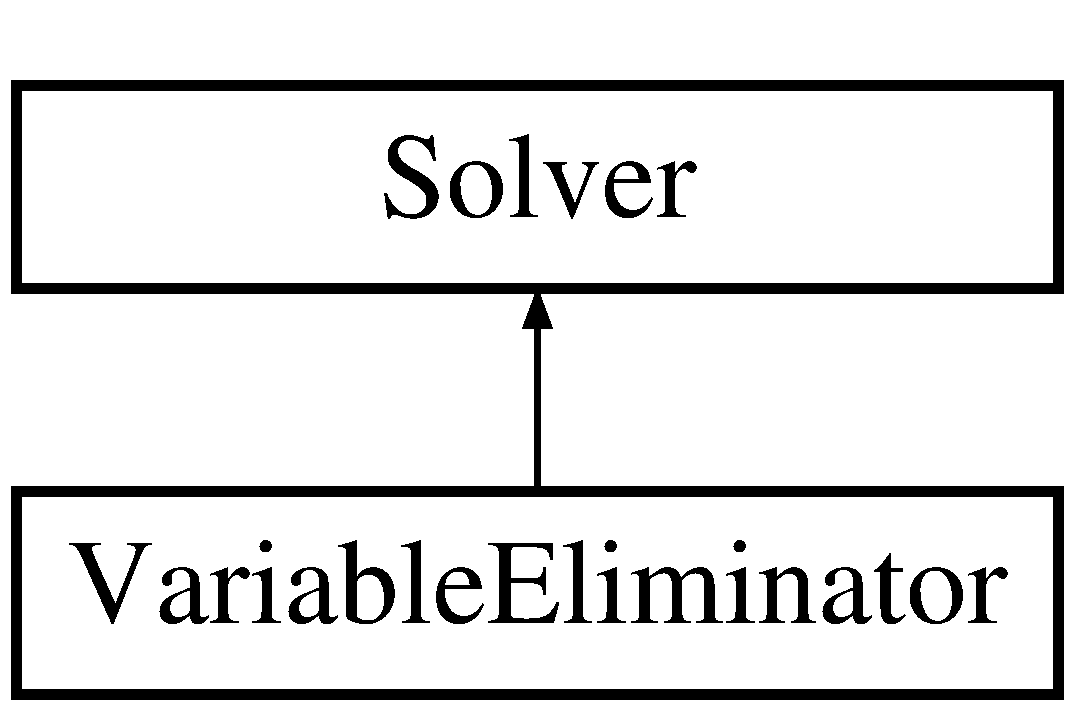
\includegraphics[height=2.000000cm]{classSolver}
\end{center}
\end{figure}
\subsection*{\-Public \-Member \-Functions}
\begin{DoxyCompactItemize}
\item 
\hypertarget{classSolver_a39f7b0b596e4ab7936b316e37a457035}{{\bfseries \-Solver} (\hyperlink{classCNode}{\-C\-Node} $\ast$node, simplification\-\_\-level level, map$<$ \hyperlink{classTerm}{\-Term} $\ast$, \hyperlink{classSatValue}{\-Sat\-Value} $>$ $\ast$assignments=\-N\-U\-L\-L, bool use\-\_\-dnf=false)}\label{classSolver_a39f7b0b596e4ab7936b316e37a457035}

\item 
\hypertarget{classSolver_a0d11a686e70c88fb02cb3556952f9589}{{\bfseries \-Solver} (\hyperlink{classCNode}{\-C\-Node} $\ast$node, \hyperlink{classCNode}{\-C\-Node} $\ast$assumptions, simplification\-\_\-level level, map$<$ \hyperlink{classTerm}{\-Term} $\ast$, \hyperlink{classSatValue}{\-Sat\-Value} $>$ $\ast$assignments=\-N\-U\-L\-L)}\label{classSolver_a0d11a686e70c88fb02cb3556952f9589}

\item 
\hypertarget{classSolver_a75acae58b51db12008c3128c37b0ef9a}{\hyperlink{classCNode}{\-C\-Node} $\ast$ {\bfseries solve} (\hyperlink{classCNode}{\-C\-Node} $\ast$node, \hyperlink{classCNode}{\-C\-Node} $\ast$assumptions, simplification\-\_\-level level, map$<$ \hyperlink{classTerm}{\-Term} $\ast$, \hyperlink{classSatValue}{\-Sat\-Value} $>$ $\ast$assignments)}\label{classSolver_a75acae58b51db12008c3128c37b0ef9a}

\item 
\hypertarget{classSolver_a7b24ed5645557b5c44aef05b265bf1ca}{\hyperlink{classCNode}{\-C\-Node} $\ast$ {\bfseries get\-\_\-result} ()}\label{classSolver_a7b24ed5645557b5c44aef05b265bf1ca}

\item 
\hypertarget{classSolver_a59e014be51c7dedaf0ea98357a70b158}{string {\bfseries get\-\_\-stats} ()}\label{classSolver_a59e014be51c7dedaf0ea98357a70b158}

\end{DoxyCompactItemize}
\subsection*{\-Static \-Public \-Member \-Functions}
\begin{DoxyCompactItemize}
\item 
\hypertarget{classSolver_acf62b72a293cc34ab8c87f17272a8c04}{static bool {\bfseries implies} (\hyperlink{classCNode}{\-C\-Node} $\ast$node1, \hyperlink{classCNode}{\-C\-Node} $\ast$node2)}\label{classSolver_acf62b72a293cc34ab8c87f17272a8c04}

\item 
\hypertarget{classSolver_aa8c6de3271be1d8cd99abafe45202a8f}{static bool {\bfseries equivalent} (\hyperlink{classCNode}{\-C\-Node} $\ast$node1, \hyperlink{classCNode}{\-C\-Node} $\ast$node2)}\label{classSolver_aa8c6de3271be1d8cd99abafe45202a8f}

\item 
\hypertarget{classSolver_ac86336f7c37d7eac95df6d58403e5d65}{static \hyperlink{classCNode}{\-C\-Node} $\ast$ {\bfseries get\-\_\-relevant\-\_\-background} (\hyperlink{classCNode}{\-C\-Node} $\ast$background, \hyperlink{classCNode}{\-C\-Node} $\ast$formula\-\_\-to\-\_\-simplify)}\label{classSolver_ac86336f7c37d7eac95df6d58403e5d65}

\end{DoxyCompactItemize}
\subsection*{\-Protected \-Member \-Functions}
\begin{DoxyCompactItemize}
\item 
\hypertarget{classSolver_ac2d16c892aea8c4e83ec3941ac16fc25}{\hyperlink{classCNode}{\-C\-Node} $\ast$ {\bfseries propagate\-\_\-equalities} (\hyperlink{classCNode}{\-C\-Node} $\ast$node, \hyperlink{classCNode}{\-C\-Node} $\ast$\&active\-\_\-constraint)}\label{classSolver_ac2d16c892aea8c4e83ec3941ac16fc25}

\item 
\hypertarget{classSolver_a71032cd9586a44c6eadd87333661f429}{void {\bfseries add\-\_\-to\-\_\-replacement\-\_\-map} (\hyperlink{classTerm}{\-Term} $\ast$to\-\_\-replace, \hyperlink{classTerm}{\-Term} $\ast$replacement, map$<$ \hyperlink{classTerm}{\-Term} $\ast$, \hyperlink{classTerm}{\-Term} $\ast$ $>$ \&replacement\-\_\-map)}\label{classSolver_a71032cd9586a44c6eadd87333661f429}

\end{DoxyCompactItemize}
\subsection*{\-Protected \-Attributes}
\begin{DoxyCompactItemize}
\item 
\hypertarget{classSolver_acab17162109917b090e1bb65db45410d}{int {\bfseries fresh\-\_\-var\-\_\-counter}}\label{classSolver_acab17162109917b090e1bb65db45410d}

\item 
\hypertarget{classSolver_a8bfe57e04a9266e094809eff9dac3b4d}{int {\bfseries solve\-\_\-count}}\label{classSolver_a8bfe57e04a9266e094809eff9dac3b4d}

\item 
\hypertarget{classSolver_acce9bd07ac7b9867f61526fff4841e05}{int {\bfseries literal\-\_\-count}}\label{classSolver_acce9bd07ac7b9867f61526fff4841e05}

\item 
\hypertarget{classSolver_a5b8a47d0b6d3c369820e61508a31d0d8}{int {\bfseries clause\-\_\-cache\-\_\-hit\-\_\-count}}\label{classSolver_a5b8a47d0b6d3c369820e61508a31d0d8}

\item 
\hypertarget{classSolver_ab06796fb4247203c201e1f82665c90b1}{int {\bfseries cache\-\_\-hits}}\label{classSolver_ab06796fb4247203c201e1f82665c90b1}

\item 
\hypertarget{classSolver_abe0ba64278604bddcb509c184aa0c67f}{int {\bfseries solve\-\_\-time}}\label{classSolver_abe0ba64278604bddcb509c184aa0c67f}

\item 
\hypertarget{classSolver_ab06ffb6630a36974bc3739cbd9024cb1}{int {\bfseries imply\-\_\-time}}\label{classSolver_ab06ffb6630a36974bc3739cbd9024cb1}

\item 
\hypertarget{classSolver_aa704e3e86465b7a38f58f792d9ffdb6b}{int {\bfseries num\-\_\-imply}}\label{classSolver_aa704e3e86465b7a38f58f792d9ffdb6b}

\item 
\hypertarget{classSolver_ab36720ab77cd7abd075fd0aaf6e40f22}{\hyperlink{classCNode}{\-C\-Node} $\ast$ {\bfseries res}}\label{classSolver_ab36720ab77cd7abd075fd0aaf6e40f22}

\end{DoxyCompactItemize}
\subsection*{\-Friends}
\begin{DoxyCompactItemize}
\item 
\hypertarget{classSolver_ace1aed02802f62c643a37b8a67e67bee}{class {\bfseries \-Interaction\-Manager}}\label{classSolver_ace1aed02802f62c643a37b8a67e67bee}

\item 
\hypertarget{classSolver_a16b09189cdaf88044be661f54a1313a7}{class {\bfseries \-Query\-Comparator}}\label{classSolver_a16b09189cdaf88044be661f54a1313a7}

\item 
\hypertarget{classSolver_a56fe9a9a7bc899066de30f41d508f524}{class {\bfseries \-Clause\-Solve}}\label{classSolver_a56fe9a9a7bc899066de30f41d508f524}

\item 
\hypertarget{classSolver_aa97b604ea37345da6b2414f0892e2664}{class {\bfseries \-Variable\-Eliminator}}\label{classSolver_aa97b604ea37345da6b2414f0892e2664}

\end{DoxyCompactItemize}


\-The documentation for this class was generated from the following files\-:\begin{DoxyCompactItemize}
\item 
solver/\-Solver.\-h\item 
solver/\-Solver.\-cpp\end{DoxyCompactItemize}

\hypertarget{structstd_1_1hash_3_01CNode_01_5_01_4}{\section{std\-:\-:hash$<$ \-C\-Node $\ast$ $>$ \-Struct \-Template \-Reference}
\label{structstd_1_1hash_3_01CNode_01_5_01_4}\index{std\-::hash$<$ C\-Node $\ast$ $>$@{std\-::hash$<$ C\-Node $\ast$ $>$}}
}
\subsection*{\-Public \-Member \-Functions}
\begin{DoxyCompactItemize}
\item 
\hypertarget{structstd_1_1hash_3_01CNode_01_5_01_4_ad1c3a9c242bf47254cb9718ceca6ef1a}{size\-\_\-t {\bfseries operator()} (const \hyperlink{classCNode}{\-C\-Node} $\ast$const \&x) const }\label{structstd_1_1hash_3_01CNode_01_5_01_4_ad1c3a9c242bf47254cb9718ceca6ef1a}

\end{DoxyCompactItemize}
\subsubsection*{template$<$$>$ struct std\-::hash$<$ C\-Node $\ast$ $>$}



\-The documentation for this struct was generated from the following file\-:\begin{DoxyCompactItemize}
\item 
cnode/\-C\-Node.\-h\end{DoxyCompactItemize}

\hypertarget{structstd_1_1hash_3_01Constraint_01_4}{\section{std\-:\-:hash$<$ \-Constraint $>$ \-Struct \-Template \-Reference}
\label{structstd_1_1hash_3_01Constraint_01_4}\index{std\-::hash$<$ Constraint $>$@{std\-::hash$<$ Constraint $>$}}
}
\subsection*{\-Public \-Member \-Functions}
\begin{DoxyCompactItemize}
\item 
\hypertarget{structstd_1_1hash_3_01Constraint_01_4_a72d6d1680af85773821b5b55d3575591}{size\-\_\-t {\bfseries operator()} (const \hyperlink{classConstraint}{\-Constraint} \&x) const }\label{structstd_1_1hash_3_01Constraint_01_4_a72d6d1680af85773821b5b55d3575591}

\end{DoxyCompactItemize}
\subsubsection*{template$<$$>$ struct std\-::hash$<$ Constraint $>$}



\-The documentation for this struct was generated from the following file\-:\begin{DoxyCompactItemize}
\item 
\-Constraint.\-h\end{DoxyCompactItemize}

\hypertarget{structstd_1_1hash_3_01Equation_01_5_01_4}{\section{std\-:\-:hash$<$ \-Equation $\ast$ $>$ \-Struct \-Template \-Reference}
\label{structstd_1_1hash_3_01Equation_01_5_01_4}\index{std\-::hash$<$ Equation $\ast$ $>$@{std\-::hash$<$ Equation $\ast$ $>$}}
}


{\ttfamily \#include $<$\-Equation.\-h$>$}

\subsection*{\-Public \-Member \-Functions}
\begin{DoxyCompactItemize}
\item 
\hypertarget{structstd_1_1hash_3_01Equation_01_5_01_4_a4a530b22a22644cd1eaadb952d8451d1}{size\-\_\-t {\bfseries operator()} (const \hyperlink{classEquation}{\-Equation} $\ast$const \&x) const }\label{structstd_1_1hash_3_01Equation_01_5_01_4_a4a530b22a22644cd1eaadb952d8451d1}

\end{DoxyCompactItemize}


\subsection{\-Detailed \-Description}
\subsubsection*{template$<$$>$struct std\-::hash$<$ Equation $\ast$ $>$}

\-Explicit template specialization of hash of a string class, which just uses the internal char$\ast$ representation as a wrapper. 

\-The documentation for this struct was generated from the following file\-:\begin{DoxyCompactItemize}
\item 
solver/\-Equation.\-h\end{DoxyCompactItemize}

\hypertarget{structstd_1_1hash_3_01pair_3_01int_00_01CNode_01_5_01_4_01_4}{\section{std\-:\-:hash$<$ pair$<$ int, \-C\-Node $\ast$ $>$ $>$ \-Struct \-Template \-Reference}
\label{structstd_1_1hash_3_01pair_3_01int_00_01CNode_01_5_01_4_01_4}\index{std\-::hash$<$ pair$<$ int, C\-Node $\ast$ $>$ $>$@{std\-::hash$<$ pair$<$ int, C\-Node $\ast$ $>$ $>$}}
}
\subsection*{\-Public \-Member \-Functions}
\begin{DoxyCompactItemize}
\item 
\hypertarget{structstd_1_1hash_3_01pair_3_01int_00_01CNode_01_5_01_4_01_4_a050889103cade857526870c1aea3151b}{size\-\_\-t {\bfseries operator()} (const pair$<$ int, \hyperlink{classCNode}{\-C\-Node} $\ast$ $>$ \&x) const }\label{structstd_1_1hash_3_01pair_3_01int_00_01CNode_01_5_01_4_01_4_a050889103cade857526870c1aea3151b}

\end{DoxyCompactItemize}
\subsubsection*{template$<$$>$ struct std\-::hash$<$ pair$<$ int, C\-Node $\ast$ $>$ $>$}



\-The documentation for this struct was generated from the following file\-:\begin{DoxyCompactItemize}
\item 
cnode/\-C\-Node.\-h\end{DoxyCompactItemize}

\hypertarget{structstd_1_1hash_3_01Term_01_5_01_4}{\section{std\-:\-:hash$<$ \-Term $\ast$ $>$ \-Struct \-Template \-Reference}
\label{structstd_1_1hash_3_01Term_01_5_01_4}\index{std\-::hash$<$ Term $\ast$ $>$@{std\-::hash$<$ Term $\ast$ $>$}}
}
\subsection*{\-Public \-Member \-Functions}
\begin{DoxyCompactItemize}
\item 
\hypertarget{structstd_1_1hash_3_01Term_01_5_01_4_a8206545c88d483e79d57d0549522e5eb}{size\-\_\-t {\bfseries operator()} (const \hyperlink{classTerm}{\-Term} $\ast$const \&x) const }\label{structstd_1_1hash_3_01Term_01_5_01_4_a8206545c88d483e79d57d0549522e5eb}

\end{DoxyCompactItemize}
\subsubsection*{template$<$$>$ struct std\-::hash$<$ Term $\ast$ $>$}



\-The documentation for this struct was generated from the following files\-:\begin{DoxyCompactItemize}
\item 
term/\-Term.\-h\item 
term/\-Term.\-cpp\end{DoxyCompactItemize}

\hypertarget{structstd_1_1term__eq}{\section{std\-:\-:term\-\_\-eq \-Struct \-Reference}
\label{structstd_1_1term__eq}\index{std\-::term\-\_\-eq@{std\-::term\-\_\-eq}}
}
\subsection*{\-Public \-Member \-Functions}
\begin{DoxyCompactItemize}
\item 
\hypertarget{structstd_1_1term__eq_a85c53edbcb8642a5ec013983d66802a9}{bool {\bfseries operator()} (const \hyperlink{classTerm}{\-Term} $\ast$l1, const \hyperlink{classTerm}{\-Term} $\ast$l2) const }\label{structstd_1_1term__eq_a85c53edbcb8642a5ec013983d66802a9}

\end{DoxyCompactItemize}


\-The documentation for this struct was generated from the following files\-:\begin{DoxyCompactItemize}
\item 
term/\-Term.\-h\item 
term/\-Term.\-cpp\end{DoxyCompactItemize}

\hypertarget{classTerm}{\section{\-Term \-Class \-Reference}
\label{classTerm}\index{\-Term@{\-Term}}
}
\-Inheritance diagram for \-Term\-:\begin{figure}[H]
\begin{center}
\leavevmode
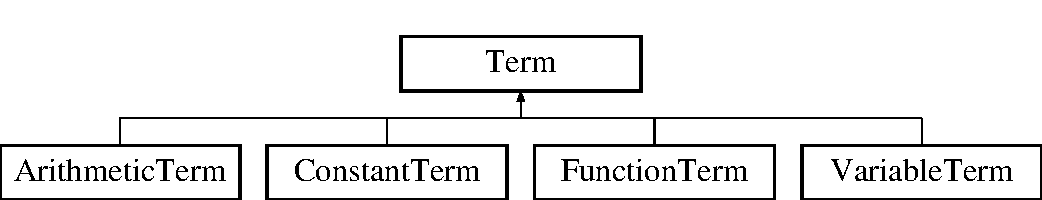
\includegraphics[height=2.000000cm]{classTerm}
\end{center}
\end{figure}
\subsection*{\-Public \-Member \-Functions}
\begin{DoxyCompactItemize}
\item 
\hypertarget{classTerm_a8ca0a73d0ef9e81f49ad5ec42b816e35}{{\footnotesize template$<$class Archive $>$ }\\void {\bfseries save} (\-Archive \&ar, const unsigned int version) const }\label{classTerm_a8ca0a73d0ef9e81f49ad5ec42b816e35}

\item 
\hypertarget{classTerm_ad922f207c28db09244f8d45bcb1189c6}{{\footnotesize template$<$class Archive $>$ }\\void {\bfseries load} (\-Archive \&ar, const unsigned int version)}\label{classTerm_ad922f207c28db09244f8d45bcb1189c6}

\item 
\hypertarget{classTerm_ad90e662483f23dc370bda049024cab90}{virtual bool {\bfseries operator==} (const \hyperlink{classTerm}{\-Term} \&other)=0}\label{classTerm_ad90e662483f23dc370bda049024cab90}

\item 
\hypertarget{classTerm_a08b3fd1f3988bccfe4a0675950adc86d}{virtual string {\bfseries to\-\_\-string} ()=0}\label{classTerm_a08b3fd1f3988bccfe4a0675950adc86d}

\item 
\hypertarget{classTerm_aeecf09df025c1f11f9f2457601b7d2a3}{term\-\_\-type {\bfseries get\-\_\-term\-\_\-type} ()}\label{classTerm_aeecf09df025c1f11f9f2457601b7d2a3}

\item 
\hypertarget{classTerm_a7da6da9de3176adac3df498fb73500fe}{bool {\bfseries is\-\_\-specialized} ()}\label{classTerm_a7da6da9de3176adac3df498fb73500fe}

\item 
\hypertarget{classTerm_a43d1547013fedd578452e513c2798f64}{int {\bfseries get\-\_\-specialization} ()}\label{classTerm_a43d1547013fedd578452e513c2798f64}

\item 
\hypertarget{classTerm_ac28d94a18f1369f6c9367660fc99552c}{term\-\_\-attribute\-\_\-type {\bfseries get\-\_\-attribute} ()}\label{classTerm_ac28d94a18f1369f6c9367660fc99552c}

\item 
\hypertarget{classTerm_a743de302324fd2eca4d4dad0b03447ee}{string {\bfseries get\-\_\-attribute\-\_\-string} ()}\label{classTerm_a743de302324fd2eca4d4dad0b03447ee}

\item 
\hypertarget{classTerm_a44fb8f8aba38e8363c98be7c46a9827d}{void {\bfseries get\-\_\-attributes} (set$<$ \hyperlink{classCNode}{\-C\-Node} $\ast$ $>$ \&attributes)}\label{classTerm_a44fb8f8aba38e8363c98be7c46a9827d}

\item 
\hypertarget{classTerm_ae3d488f52f259da2b203ae425e0a42be}{void {\bfseries set\-\_\-attribute} (term\-\_\-attribute\-\_\-type ta)}\label{classTerm_ae3d488f52f259da2b203ae425e0a42be}

\item 
\hypertarget{classTerm_a9cb1e2671d02520182861808f692fbce}{size\-\_\-t {\bfseries hash\-\_\-code} ()}\label{classTerm_a9cb1e2671d02520182861808f692fbce}

\item 
\hypertarget{classTerm_afa34fcef6d5c648c36108eb1afbbffb1}{void {\bfseries get\-\_\-nested\-\_\-vars} (set$<$ int $>$ \&vars)}\label{classTerm_afa34fcef6d5c648c36108eb1afbbffb1}

\item 
\hypertarget{classTerm_a50ac643f14b8a613afcb73c25f8a6a70}{void {\bfseries get\-\_\-nested\-\_\-terms} (set$<$ \hyperlink{classTerm}{\-Term} $\ast$ $>$ \&terms, bool include\-\_\-function\-\_\-subterms=true, bool include\-\_\-constants=true)}\label{classTerm_a50ac643f14b8a613afcb73c25f8a6a70}

\item 
\hypertarget{classTerm_acd2d1f7f504ce1c18b790366f1b84c7b}{virtual \hyperlink{classTerm}{\-Term} $\ast$ {\bfseries substitute} (map$<$ \hyperlink{classTerm}{\-Term} $\ast$, \hyperlink{classTerm}{\-Term} $\ast$ $>$ \&subs)=0}\label{classTerm_acd2d1f7f504ce1c18b790366f1b84c7b}

\item 
\hypertarget{classTerm_ad1d5f30b5f3e2863bfbf732ae3729694}{\hyperlink{classTerm}{\-Term} $\ast$ {\bfseries substitute} (\hyperlink{classTerm}{\-Term} $\ast$($\ast$sub\-\_\-func)(\hyperlink{classTerm}{\-Term} $\ast$t))}\label{classTerm_ad1d5f30b5f3e2863bfbf732ae3729694}

\item 
\hypertarget{classTerm_a60bad8e42e0062d7ba1513ce60a5e578}{virtual \hyperlink{classTerm}{\-Term} $\ast$ {\bfseries substitute} (\hyperlink{classTerm}{\-Term} $\ast$($\ast$sub\-\_\-func)(\hyperlink{classTerm}{\-Term} $\ast$t, void $\ast$data), void $\ast$my\-\_\-data)}\label{classTerm_a60bad8e42e0062d7ba1513ce60a5e578}

\item 
\hypertarget{classTerm_aff7d56374e09bfc139e1830318d03d51}{void {\bfseries clear\-\_\-representatives} ()}\label{classTerm_aff7d56374e09bfc139e1830318d03d51}

\item 
\hypertarget{classTerm_a9a1d4db8f0ce99e2f7056f6211858f8c}{\hyperlink{classTerm}{\-Term} $\ast$ {\bfseries replace\-\_\-term} (\hyperlink{classTerm}{\-Term} $\ast$old\-\_\-term, \hyperlink{classTerm}{\-Term} $\ast$new\-\_\-term)}\label{classTerm_a9a1d4db8f0ce99e2f7056f6211858f8c}

\item 
\hypertarget{classTerm_a1e419cac626845aa67865a120cd4a47d}{void {\bfseries get\-\_\-vars} (set$<$ string $>$ \&vars)}\label{classTerm_a1e419cac626845aa67865a120cd4a47d}

\item 
\hypertarget{classTerm_afa91787e5b03d2905d260ba4b62a2316}{void {\bfseries get\-\_\-vars} (set$<$ int $>$ \&vars)}\label{classTerm_afa91787e5b03d2905d260ba4b62a2316}

\item 
\hypertarget{classTerm_a91c02985966cc4585bacce557d88fb40}{void {\bfseries get\-\_\-vars} (set$<$ \hyperlink{classTerm}{\-Term} $\ast$ $>$ \&vars)}\label{classTerm_a91c02985966cc4585bacce557d88fb40}

\item 
\hypertarget{classTerm_a7dd250f12b42f9fd5e4b5d1c69f3de54}{bool {\bfseries contains\-\_\-term} (\hyperlink{classTerm}{\-Term} $\ast$t)}\label{classTerm_a7dd250f12b42f9fd5e4b5d1c69f3de54}

\item 
\hypertarget{classTerm_a14c34b9e24c7030786b690edf342dc19}{bool {\bfseries contains\-\_\-term} (set$<$ \hyperlink{classTerm}{\-Term} $\ast$ $>$ \&terms)}\label{classTerm_a14c34b9e24c7030786b690edf342dc19}

\item 
\hypertarget{classTerm_a7a1e02886dc59a52ebadc5a4d26dad7b}{bool {\bfseries contains\-\_\-var} (int var\-\_\-id)}\label{classTerm_a7a1e02886dc59a52ebadc5a4d26dad7b}

\item 
\hypertarget{classTerm_a6d0357f6ea3cde2c7985f1ea173eb8fe}{void {\bfseries get\-\_\-all\-\_\-fun\-\_\-ids} (set$<$ int $>$ \&ids)}\label{classTerm_a6d0357f6ea3cde2c7985f1ea173eb8fe}

\item 
\hypertarget{classTerm_ae7b58efd92e0f765751b75ef3b1e8bdd}{void {\bfseries get\-\_\-all\-\_\-arguments} (int fun\-\_\-id, int arg\-\_\-num, set$<$ \hyperlink{classTerm}{\-Term} $\ast$ $>$ \&args)}\label{classTerm_ae7b58efd92e0f765751b75ef3b1e8bdd}

\item 
\hypertarget{classTerm_a1d2acc1e9bafa53dccd3a2a36e97a078}{void {\bfseries get\-\_\-all\-\_\-first\-\_\-arguments} (set$<$ int $>$ \&fn\-\_\-ids, map$<$ int, set$<$ \hyperlink{classTerm}{\-Term} $\ast$ $>$ $>$ \&fn\-\_\-id\-\_\-to\-\_\-first\-\_\-arg)}\label{classTerm_a1d2acc1e9bafa53dccd3a2a36e97a078}

\item 
\hypertarget{classTerm_a97c1a43cbabf5b8b53d58cae43dcc355}{\hyperlink{classTerm}{\-Term} $\ast$ {\bfseries replace\-\_\-argument} (int fun\-\_\-id, int arg\-\_\-num, \hyperlink{classTerm}{\-Term} $\ast$replacement)}\label{classTerm_a97c1a43cbabf5b8b53d58cae43dcc355}

\item 
\hypertarget{classTerm_ab471816cb9b296a9bb3f21ab44a4768f}{\hyperlink{classTerm}{\-Term} $\ast$ {\bfseries replace\-\_\-first\-\_\-argument} (map$<$ int, \hyperlink{classTerm}{\-Term} $\ast$ $>$ \&fun\-\_\-id\-\_\-to\-\_\-replacements)}\label{classTerm_ab471816cb9b296a9bb3f21ab44a4768f}

\item 
\hypertarget{classTerm_a37733a2ff1a1b24bd9f4fd3000a88a19}{bool {\bfseries shares\-\_\-subterms} (\hyperlink{classTerm}{\-Term} $\ast$other)}\label{classTerm_a37733a2ff1a1b24bd9f4fd3000a88a19}

\item 
\hypertarget{classTerm_a56c02b4c370ddd87d04318452bd60d36}{bool {\bfseries contains\-\_\-var} ()}\label{classTerm_a56c02b4c370ddd87d04318452bd60d36}

\item 
\hypertarget{classTerm_ac63abe07c0ae7b48340d9aea94d83249}{\hyperlink{classTerm}{\-Term} $\ast$ {\bfseries rename\-\_\-variable} (int old\-\_\-var\-\_\-id, int new\-\_\-var\-\_\-id)}\label{classTerm_ac63abe07c0ae7b48340d9aea94d83249}

\item 
\hypertarget{classTerm_abb1d7100eaa04d92c18a484429e124f2}{\hyperlink{classTerm}{\-Term} $\ast$ {\bfseries rename\-\_\-variables} (map$<$ int, int $>$ \&replacements)}\label{classTerm_abb1d7100eaa04d92c18a484429e124f2}

\item 
\hypertarget{classTerm_aba4768b8f008757184e6c4037e33ed43}{\hyperlink{classTerm}{\-Term} $\ast$ {\bfseries flip\-\_\-sign} ()}\label{classTerm_aba4768b8f008757184e6c4037e33ed43}

\item 
\hypertarget{classTerm_a7b6ce6dafbe7523c8d13e0d216058a79}{\hyperlink{classTerm}{\-Term} $\ast$ {\bfseries multiply} (long int factor)}\label{classTerm_a7b6ce6dafbe7523c8d13e0d216058a79}

\item 
\hypertarget{classTerm_a2877a445223a37626aa185578814d596}{\hyperlink{classTerm}{\-Term} $\ast$ {\bfseries add} (long int constant)}\label{classTerm_a2877a445223a37626aa185578814d596}

\item 
\hypertarget{classTerm_a87af3d4bb0b9233c14ec51550d5271db}{\hyperlink{classTerm}{\-Term} $\ast$ {\bfseries add} (\hyperlink{classTerm}{\-Term} $\ast$t)}\label{classTerm_a87af3d4bb0b9233c14ec51550d5271db}

\item 
\hypertarget{classTerm_add8b115657cd9981f3a849e132253523}{\hyperlink{classTerm}{\-Term} $\ast$ {\bfseries subtract} (\hyperlink{classTerm}{\-Term} $\ast$t)}\label{classTerm_add8b115657cd9981f3a849e132253523}

\item 
\hypertarget{classTerm_abce229c606237df1e1ea4c546d0253da}{\hyperlink{classTerm}{\-Term} $\ast$ {\bfseries evalute\-\_\-term} (map$<$ \hyperlink{classTerm}{\-Term} $\ast$, \hyperlink{classSatValue}{\-Sat\-Value} $>$ \&assignments)}\label{classTerm_abce229c606237df1e1ea4c546d0253da}

\item 
\hypertarget{classTerm_a049329c5989dcb2587947806ac9c63ac}{\hyperlink{classTerm}{\-Term} $\ast$ {\bfseries multiply} (\hyperlink{classTerm}{\-Term} $\ast$t)}\label{classTerm_a049329c5989dcb2587947806ac9c63ac}

\end{DoxyCompactItemize}
\subsection*{\-Static \-Public \-Member \-Functions}
\begin{DoxyCompactItemize}
\item 
\hypertarget{classTerm_a67a37dab80c22a0ad179745522e4684d}{static \hyperlink{classTerm}{\-Term} $\ast$ {\bfseries get\-\_\-term} (\hyperlink{classTerm}{\-Term} $\ast$t)}\label{classTerm_a67a37dab80c22a0ad179745522e4684d}

\item 
\hypertarget{classTerm_af00fe6e59c07b99ecb1598b604b8ad34}{static \hyperlink{classTerm}{\-Term} $\ast$ {\bfseries get\-\_\-term\-\_\-nodelete} (\hyperlink{classTerm}{\-Term} $\ast$t)}\label{classTerm_af00fe6e59c07b99ecb1598b604b8ad34}

\item 
\hypertarget{classTerm_aa80cc2a16f137a15c1897509fcedff08}{static \hyperlink{classTerm}{\-Term} $\ast$ {\bfseries uniquify\-\_\-term} (\hyperlink{classTerm}{\-Term} $\ast$t)}\label{classTerm_aa80cc2a16f137a15c1897509fcedff08}

\item 
\hypertarget{classTerm_ae4db8c34d91b562ecbdbebddfc47c12b}{static void {\bfseries delete\-\_\-loaded\-\_\-terms} ()}\label{classTerm_ae4db8c34d91b562ecbdbebddfc47c12b}

\end{DoxyCompactItemize}
\subsection*{\-Public \-Attributes}
\begin{DoxyCompactItemize}
\item 
\hypertarget{classTerm_a0154fc4b2a90d16329f310faa2e42535}{size\-\_\-t {\bfseries hash\-\_\-c}}\label{classTerm_a0154fc4b2a90d16329f310faa2e42535}

\item 
\hypertarget{classTerm_ac9aaad86da37f49b7ac0fd9e561eeb2b}{term\-\_\-type {\bfseries type}}\label{classTerm_ac9aaad86da37f49b7ac0fd9e561eeb2b}

\item 
\hypertarget{classTerm_ab01e1866e9977b8c8fd76c3c601e93c0}{term\-\_\-attribute\-\_\-type {\bfseries attribute}}\label{classTerm_ab01e1866e9977b8c8fd76c3c601e93c0}

\item 
\hypertarget{classTerm_abb70538c11fc3a7af3a87bcfc32261b6}{int {\bfseries specialization\-\_\-type}}\label{classTerm_abb70538c11fc3a7af3a87bcfc32261b6}

\item 
\hypertarget{classTerm_a9d43cd23ce7d9ced12fba0c1f7bddb29}{\hyperlink{classTerm}{\-Term} $\ast$ {\bfseries representative}}\label{classTerm_a9d43cd23ce7d9ced12fba0c1f7bddb29}

\end{DoxyCompactItemize}
\subsection*{\-Static \-Public \-Attributes}
\begin{DoxyCompactItemize}
\item 
\hypertarget{classTerm_a83411382cdba54da5e43e7286e272982}{static unordered\-\_\-set$<$ \hyperlink{classTerm}{\-Term} \*
$\ast$, std\-::hash$<$ \hyperlink{classTerm}{\-Term} $\ast$ $>$\*
, \hyperlink{structstd_1_1term__eq}{term\-\_\-eq} $>$ {\bfseries terms}}\label{classTerm_a83411382cdba54da5e43e7286e272982}

\item 
\hypertarget{classTerm_aff98a6cba75cf099e005be04d56623c1}{static set$<$ \hyperlink{classTerm}{\-Term} $\ast$ $>$ {\bfseries to\-\_\-delete}}\label{classTerm_aff98a6cba75cf099e005be04d56623c1}

\end{DoxyCompactItemize}
\subsection*{\-Static \-Protected \-Member \-Functions}
\begin{DoxyCompactItemize}
\item 
\hypertarget{classTerm_ab640d41ead4b1e4bb98c4a31bfe7e170}{static void {\bfseries clear} ()}\label{classTerm_ab640d41ead4b1e4bb98c4a31bfe7e170}

\end{DoxyCompactItemize}
\subsection*{\-Friends}
\begin{DoxyCompactItemize}
\item 
\hypertarget{classTerm_ac98d07dd8f7b70e16ccb9a01abf56b9c}{class {\bfseries boost\-::serialization\-::access}}\label{classTerm_ac98d07dd8f7b70e16ccb9a01abf56b9c}

\item 
\hypertarget{classTerm_a0657a422d4ddc5f4a0ff56931b7d2767}{class {\bfseries \-C\-Node}}\label{classTerm_a0657a422d4ddc5f4a0ff56931b7d2767}

\end{DoxyCompactItemize}


\-The documentation for this class was generated from the following files\-:\begin{DoxyCompactItemize}
\item 
term/\-Term.\-h\item 
term/\-Term.\-cpp\end{DoxyCompactItemize}

\hypertarget{classTermComparator}{\section{\-Term\-Comparator \-Class \-Reference}
\label{classTermComparator}\index{\-Term\-Comparator@{\-Term\-Comparator}}
}
\subsection*{\-Public \-Member \-Functions}
\begin{DoxyCompactItemize}
\item 
\hypertarget{classTermComparator_a49693a19b255f6943722ea8d2bad9d1e}{bool {\bfseries operator()} (const \hyperlink{classTerm}{\-Term} $\ast$const \&\-\_\-q1, const \hyperlink{classTerm}{\-Term} $\ast$const \&\-\_\-q2)}\label{classTermComparator_a49693a19b255f6943722ea8d2bad9d1e}

\end{DoxyCompactItemize}


\-The documentation for this class was generated from the following file\-:\begin{DoxyCompactItemize}
\item 
solver/\-Interaction\-Manager.\-h\end{DoxyCompactItemize}

\hypertarget{classTrue}{\section{\-True \-Class \-Reference}
\label{classTrue}\index{\-True@{\-True}}
}
\-Inheritance diagram for \-True\-:\begin{figure}[H]
\begin{center}
\leavevmode
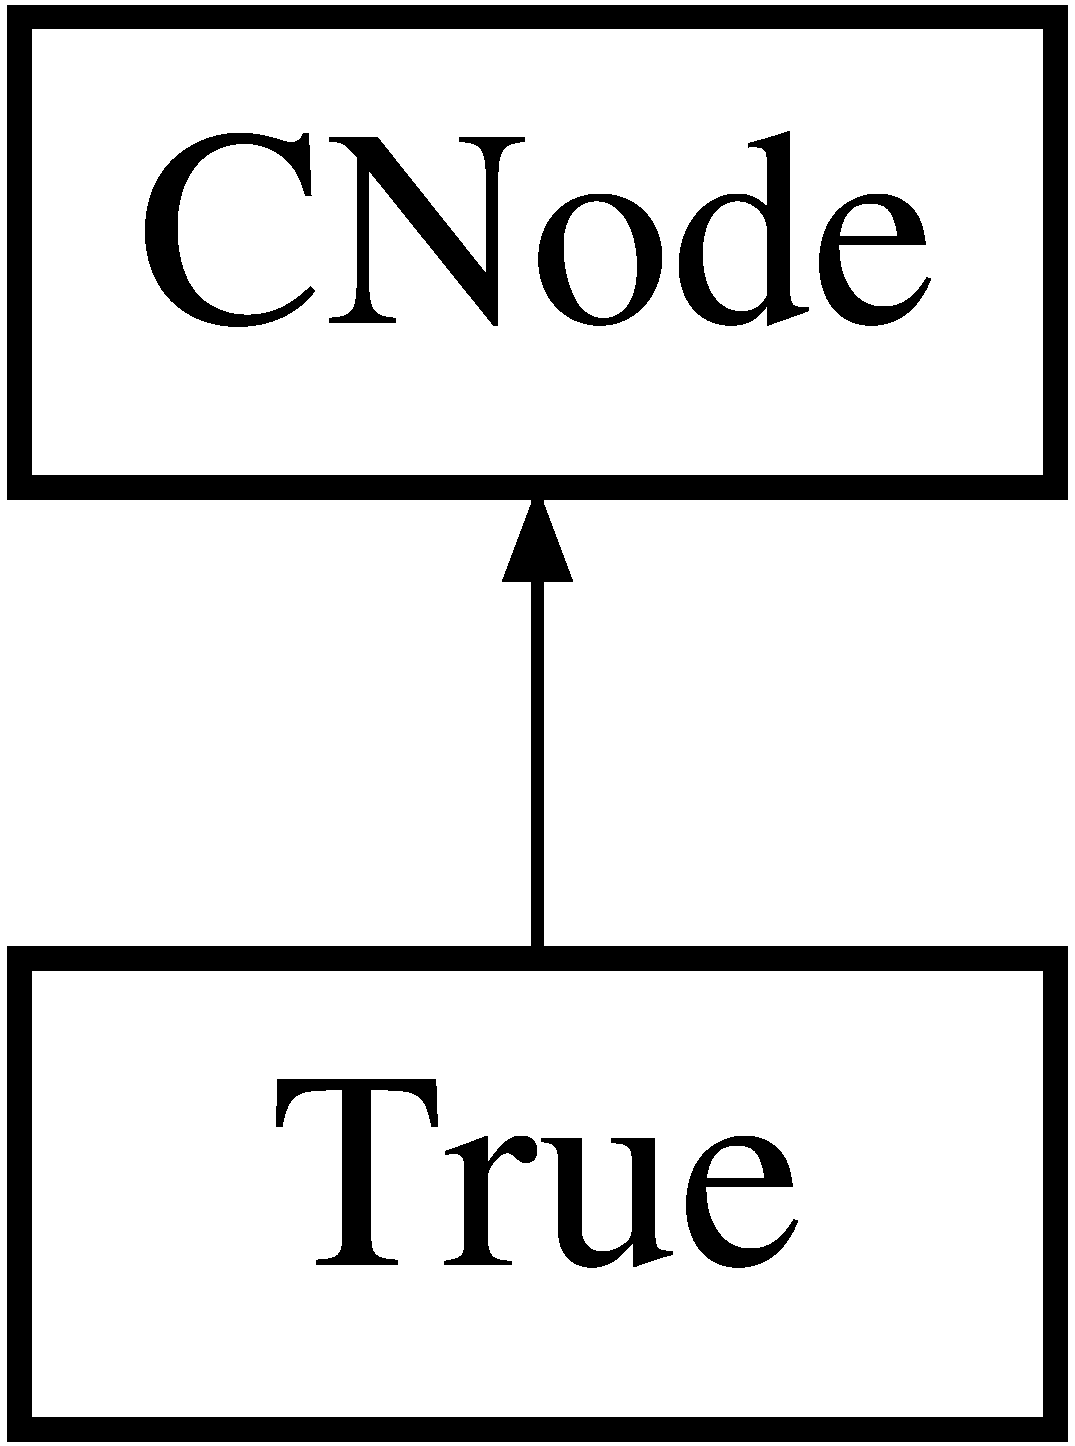
\includegraphics[height=2.000000cm]{classTrue}
\end{center}
\end{figure}
\subsection*{\-Public \-Member \-Functions}
\begin{DoxyCompactItemize}
\item 
\hypertarget{classTrue_a010be15891ada56b4fee29d56089f177}{virtual bool {\bfseries operator==} (const \hyperlink{classCNode}{\-C\-Node} \&other)}\label{classTrue_a010be15891ada56b4fee29d56089f177}

\item 
\hypertarget{classTrue_a73d36085cd7162481960115489437f64}{virtual string {\bfseries to\-\_\-string} ()}\label{classTrue_a73d36085cd7162481960115489437f64}

\item 
\hypertarget{classTrue_aa8bb181553bce8aeec1962862d8d8564}{virtual \hyperlink{classCNode}{\-C\-Node} $\ast$ {\bfseries substitute} (map$<$ \hyperlink{classTerm}{\-Term} $\ast$, \hyperlink{classTerm}{\-Term} $\ast$ $>$ \&subs)}\label{classTrue_aa8bb181553bce8aeec1962862d8d8564}

\end{DoxyCompactItemize}
\subsection*{\-Static \-Public \-Member \-Functions}
\begin{DoxyCompactItemize}
\item 
\hypertarget{classTrue_ada3b9d8de5887454efeeaa0e43576a01}{static \hyperlink{classCNode}{\-C\-Node} $\ast$ {\bfseries make} ()}\label{classTrue_ada3b9d8de5887454efeeaa0e43576a01}

\end{DoxyCompactItemize}
\subsection*{\-Friends}
\begin{DoxyCompactItemize}
\item 
\hypertarget{classTrue_a0657a422d4ddc5f4a0ff56931b7d2767}{class {\bfseries \-C\-Node}}\label{classTrue_a0657a422d4ddc5f4a0ff56931b7d2767}

\item 
\hypertarget{classTrue_ac98d07dd8f7b70e16ccb9a01abf56b9c}{class {\bfseries boost\-::serialization\-::access}}\label{classTrue_ac98d07dd8f7b70e16ccb9a01abf56b9c}

\end{DoxyCompactItemize}


\-The documentation for this class was generated from the following files\-:\begin{DoxyCompactItemize}
\item 
cnode/\-True.\-h\item 
cnode/\-True.\-cpp\end{DoxyCompactItemize}

\hypertarget{classUniversalInstantiator}{\section{\-Universal\-Instantiator \-Class \-Reference}
\label{classUniversalInstantiator}\index{\-Universal\-Instantiator@{\-Universal\-Instantiator}}
}
\subsection*{\-Public \-Member \-Functions}
\begin{DoxyCompactItemize}
\item 
\hypertarget{classUniversalInstantiator_abceb99337d55da377297b791c924774c}{{\bfseries \-Universal\-Instantiator} (\hyperlink{classCNode}{\-C\-Node} $\ast$node, bool $\ast$success=\-N\-U\-L\-L)}\label{classUniversalInstantiator_abceb99337d55da377297b791c924774c}

\item 
\hypertarget{classUniversalInstantiator_aa0fb9868d1b7fef64436134c506b6c85}{\hyperlink{classCNode}{\-C\-Node} $\ast$ {\bfseries get\-\_\-constraint} ()}\label{classUniversalInstantiator_aa0fb9868d1b7fef64436134c506b6c85}

\end{DoxyCompactItemize}


\-The documentation for this class was generated from the following files\-:\begin{DoxyCompactItemize}
\item 
solver/\-Universal\-Instantiator.\-h\item 
solver/\-Universal\-Instantiator.\-cpp\end{DoxyCompactItemize}

\hypertarget{classUnsatCoreFinder}{\section{\-Unsat\-Core\-Finder \-Class \-Reference}
\label{classUnsatCoreFinder}\index{\-Unsat\-Core\-Finder@{\-Unsat\-Core\-Finder}}
}
\subsection*{\-Public \-Member \-Functions}
\begin{DoxyCompactItemize}
\item 
\hypertarget{classUnsatCoreFinder_a16ff7e8d507aa1cb8ff27a7ae8754ad6}{{\bfseries \-Unsat\-Core\-Finder} (\hyperlink{classCNode}{\-C\-Node} $\ast$c, set$<$ \hyperlink{classCNode}{\-C\-Node} $\ast$ $>$ \&must\-\_\-assignments)}\label{classUnsatCoreFinder_a16ff7e8d507aa1cb8ff27a7ae8754ad6}

\item 
\hypertarget{classUnsatCoreFinder_a51bc021408dd10564173025140d0fe1c}{\hyperlink{classCNode}{\-C\-Node} $\ast$ {\bfseries get\-\_\-unsat\-\_\-core} ()}\label{classUnsatCoreFinder_a51bc021408dd10564173025140d0fe1c}

\end{DoxyCompactItemize}


\-The documentation for this class was generated from the following files\-:\begin{DoxyCompactItemize}
\item 
solver/\-Unsat\-Core\-Finder.\-h\item 
solver/\-Unsat\-Core\-Finder.\-cpp\end{DoxyCompactItemize}

\hypertarget{classVariableEliminator}{\section{\-Variable\-Eliminator \-Class \-Reference}
\label{classVariableEliminator}\index{\-Variable\-Eliminator@{\-Variable\-Eliminator}}
}
\-Inheritance diagram for \-Variable\-Eliminator\-:\begin{figure}[H]
\begin{center}
\leavevmode
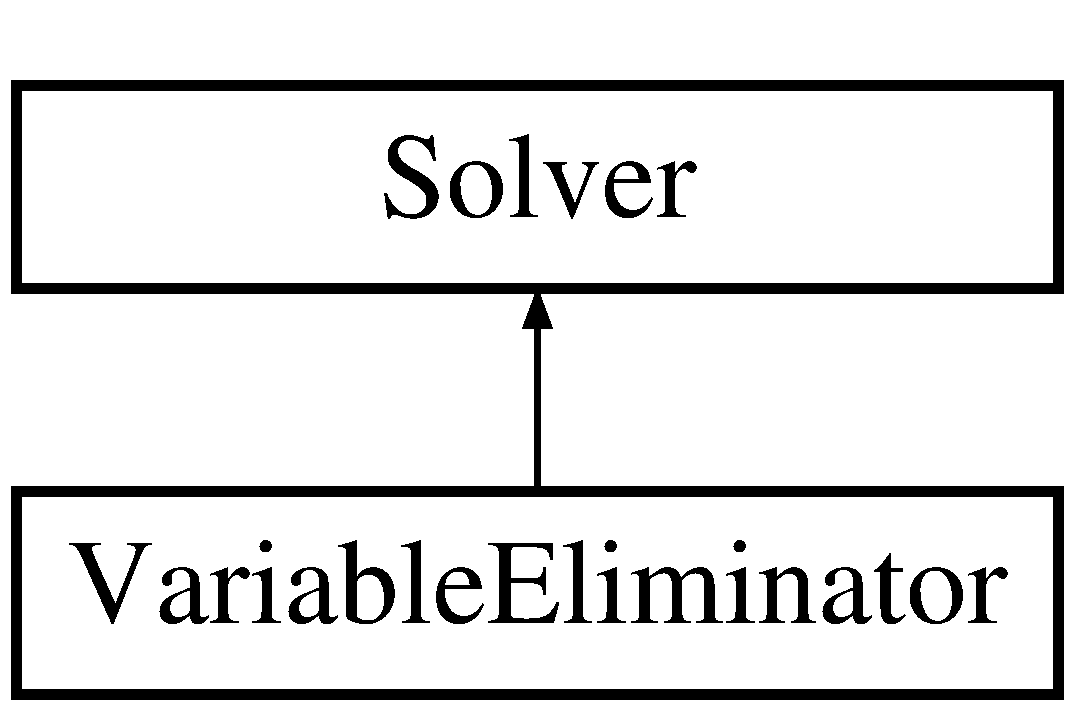
\includegraphics[height=2.000000cm]{classVariableEliminator}
\end{center}
\end{figure}
\subsection*{\-Public \-Member \-Functions}
\begin{DoxyCompactItemize}
\item 
\hypertarget{classVariableEliminator_a6751413492bab4caaf0ceab3eb710098}{{\bfseries \-Variable\-Eliminator} (\hyperlink{classCNode}{\-C\-Node} $\ast$n, vector$<$ \hyperlink{classVariableTerm}{\-Variable\-Term} $\ast$ $>$ \&to\-\_\-eliminate, simplification\-\_\-level level, bool over\-\_\-approximate, bool track\-\_\-new\-\_\-inequalities=false)}\label{classVariableEliminator_a6751413492bab4caaf0ceab3eb710098}

\item 
\hypertarget{classVariableEliminator_ab6fc2ed942a6c00f9db6516e61e47ed5}{{\bfseries \-Variable\-Eliminator} (\hyperlink{classCNode}{\-C\-Node} $\ast$n, \hyperlink{classVariableTerm}{\-Variable\-Term} $\ast$to\-\_\-eliminate, simplification\-\_\-level level, bool over\-\_\-approximate, bool track\-\_\-new\-\_\-inequalities=false)}\label{classVariableEliminator_ab6fc2ed942a6c00f9db6516e61e47ed5}

\item 
\hypertarget{classVariableEliminator_aa27b290bccf655eea0c5c7eca6998232}{const map$<$ \hyperlink{classVariableTerm}{\-Variable\-Term} $\ast$, set\*
$<$ pair$<$ \hyperlink{classTerm}{\-Term} $\ast$, \hyperlink{classTerm}{\-Term} $\ast$ $>$ $>$ $>$ \& {\bfseries get\-\_\-new\-\_\-inequalities} ()}\label{classVariableEliminator_aa27b290bccf655eea0c5c7eca6998232}

\end{DoxyCompactItemize}


\-The documentation for this class was generated from the following files\-:\begin{DoxyCompactItemize}
\item 
solver/\-Variable\-Eliminator.\-h\item 
solver/\-Variable\-Eliminator.\-cpp\end{DoxyCompactItemize}

\hypertarget{classVariableTerm}{\section{\-Variable\-Term \-Class \-Reference}
\label{classVariableTerm}\index{\-Variable\-Term@{\-Variable\-Term}}
}
\-Inheritance diagram for \-Variable\-Term\-:\begin{figure}[H]
\begin{center}
\leavevmode
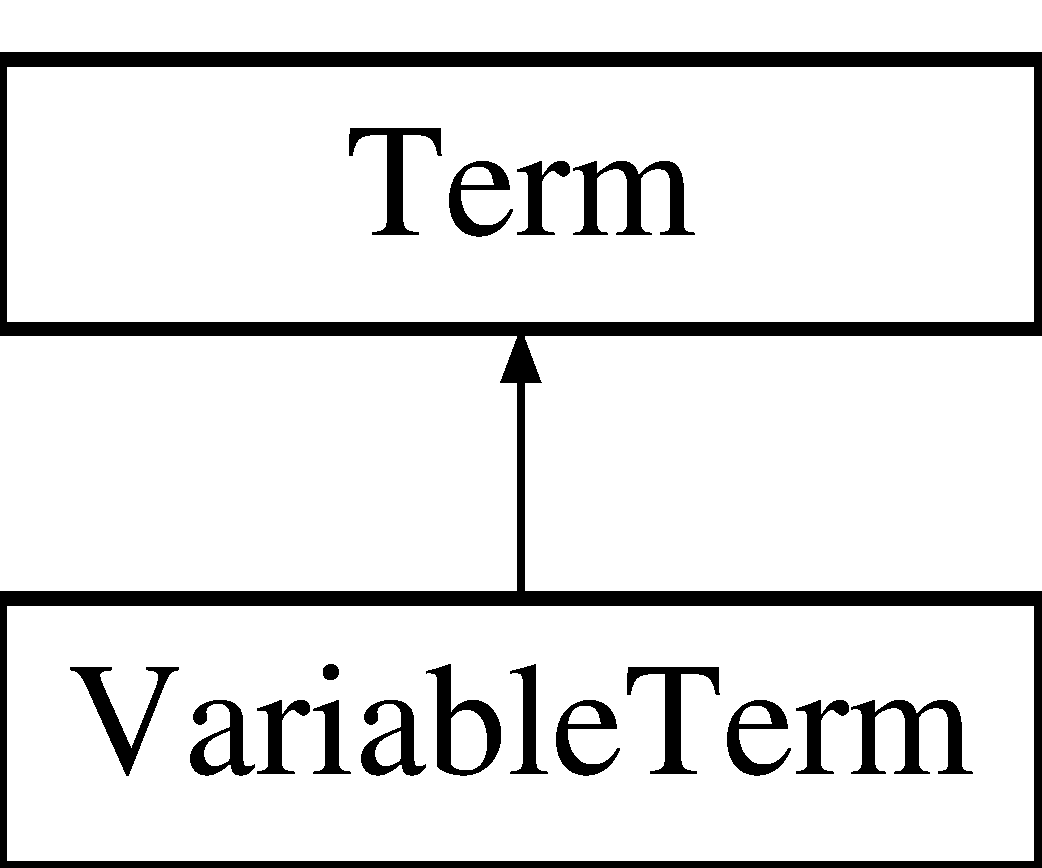
\includegraphics[height=2.000000cm]{classVariableTerm}
\end{center}
\end{figure}
\subsection*{\-Public \-Member \-Functions}
\begin{DoxyCompactItemize}
\item 
\hypertarget{classVariableTerm_abb354a4192f88f8fb1224de82a5d7218}{{\bfseries \-Variable\-Term} (int var\-\_\-id, int attribute=0)}\label{classVariableTerm_abb354a4192f88f8fb1224de82a5d7218}

\item 
\hypertarget{classVariableTerm_a16b80cc7b7f6b5889da32aac1aeba713}{virtual bool {\bfseries operator==} (const \hyperlink{classTerm}{\-Term} \&other)}\label{classVariableTerm_a16b80cc7b7f6b5889da32aac1aeba713}

\item 
\hypertarget{classVariableTerm_a4b5946494e46908a55dce15d4838d346}{virtual string {\bfseries to\-\_\-string} ()}\label{classVariableTerm_a4b5946494e46908a55dce15d4838d346}

\item 
\hypertarget{classVariableTerm_a3d975ecca51867abfc4edd826a7dbd39}{int {\bfseries get\-\_\-id\-\_\-attribute} () const }\label{classVariableTerm_a3d975ecca51867abfc4edd826a7dbd39}

\item 
\hypertarget{classVariableTerm_aae822579bca1c64486f2d7743bf5a69a}{int {\bfseries get\-\_\-var\-\_\-id} ()}\label{classVariableTerm_aae822579bca1c64486f2d7743bf5a69a}

\item 
\hypertarget{classVariableTerm_a8b53abd833b35dc25b73e2861e0c5a63}{string {\bfseries get\-\_\-name} ()}\label{classVariableTerm_a8b53abd833b35dc25b73e2861e0c5a63}

\item 
\hypertarget{classVariableTerm_a314f7345927c095d015a3c396101573d}{virtual \hyperlink{classTerm}{\-Term} $\ast$ {\bfseries substitute} (map$<$ \hyperlink{classTerm}{\-Term} $\ast$, \hyperlink{classTerm}{\-Term} $\ast$ $>$ \&subs)}\label{classVariableTerm_a314f7345927c095d015a3c396101573d}

\end{DoxyCompactItemize}
\subsection*{\-Static \-Public \-Member \-Functions}
\begin{DoxyCompactItemize}
\item 
\hypertarget{classVariableTerm_af118e2572aaf9496ab9ccebe0728fe71}{static \hyperlink{classTerm}{\-Term} $\ast$ {\bfseries make} (int id)}\label{classVariableTerm_af118e2572aaf9496ab9ccebe0728fe71}

\item 
\hypertarget{classVariableTerm_a799b5a5ff8468595c4f398a4aa654e78}{static \hyperlink{classTerm}{\-Term} $\ast$ {\bfseries make} (string name)}\label{classVariableTerm_a799b5a5ff8468595c4f398a4aa654e78}

\end{DoxyCompactItemize}
\subsection*{\-Friends}
\begin{DoxyCompactItemize}
\item 
\hypertarget{classVariableTerm_ac98d07dd8f7b70e16ccb9a01abf56b9c}{class {\bfseries boost\-::serialization\-::access}}\label{classVariableTerm_ac98d07dd8f7b70e16ccb9a01abf56b9c}

\end{DoxyCompactItemize}


\-The documentation for this class was generated from the following files\-:\begin{DoxyCompactItemize}
\item 
term/\-Variable\-Term.\-h\item 
term/\-Variable\-Term.\-cpp\end{DoxyCompactItemize}

\hypertarget{classVarMap}{\section{\-Var\-Map \-Class \-Reference}
\label{classVarMap}\index{\-Var\-Map@{\-Var\-Map}}
}
\subsection*{\-Public \-Member \-Functions}
\begin{DoxyCompactItemize}
\item 
\hypertarget{classVarMap_a642547670d6ab8148b9bbf638f953137}{int {\bfseries get\-\_\-id} (string name, bool invertible=false)}\label{classVarMap_a642547670d6ab8148b9bbf638f953137}

\item 
\hypertarget{classVarMap_a0748479f669f0977b8e3a76db1aa5d2b}{int {\bfseries get\-\_\-attrib} (int id)}\label{classVarMap_a0748479f669f0977b8e3a76db1aa5d2b}

\item 
\hypertarget{classVarMap_aa237b264636a54cb90c9eea19e3c6704}{string {\bfseries get\-\_\-name} (int id)}\label{classVarMap_aa237b264636a54cb90c9eea19e3c6704}

\item 
\hypertarget{classVarMap_ab313eba9e018928629ade3ee27af6626}{bool {\bfseries contains\-\_\-name} (string name)}\label{classVarMap_ab313eba9e018928629ade3ee27af6626}

\item 
\hypertarget{classVarMap_aafc459209a7e690c29f34f2bf3608125}{void {\bfseries get\-\_\-all\-\_\-vars} (set$<$ string $>$ \&var\-\_\-names)}\label{classVarMap_aafc459209a7e690c29f34f2bf3608125}

\item 
\hypertarget{classVarMap_ada11009e999614753d6eccb11f5ae5e3}{void {\bfseries clear} ()}\label{classVarMap_ada11009e999614753d6eccb11f5ae5e3}

\end{DoxyCompactItemize}


\-The documentation for this class was generated from the following files\-:\begin{DoxyCompactItemize}
\item 
\-Var\-Map.\-h\item 
\-Var\-Map.\-cpp\end{DoxyCompactItemize}

\hypertarget{classvec}{\section{vec$<$ \-T $>$ \-Class \-Template \-Reference}
\label{classvec}\index{vec$<$ T $>$@{vec$<$ T $>$}}
}
\subsection*{\-Public \-Types}
\begin{DoxyCompactItemize}
\item 
\hypertarget{classvec_a2534b2a9d2c8aaa686a0fd9ffbba2b74}{typedef int {\bfseries \-Key}}\label{classvec_a2534b2a9d2c8aaa686a0fd9ffbba2b74}

\item 
\hypertarget{classvec_acf60a9a9f8b3c0bb7562ad00076485c6}{typedef \-T {\bfseries \-Datum}}\label{classvec_acf60a9a9f8b3c0bb7562ad00076485c6}

\end{DoxyCompactItemize}
\subsection*{\-Public \-Member \-Functions}
\begin{DoxyCompactItemize}
\item 
\hypertarget{classvec_ad2d8eaf011ab18c61f19b50fdb3245a5}{{\bfseries vec} (int size)}\label{classvec_ad2d8eaf011ab18c61f19b50fdb3245a5}

\item 
\hypertarget{classvec_a32b79f3a6825ce05df3cccbbb1faa9b4}{{\bfseries vec} (int size, const \-T \&pad)}\label{classvec_a32b79f3a6825ce05df3cccbbb1faa9b4}

\item 
\hypertarget{classvec_ae2d0a0165045abc5413118e7a2a09ee7}{{\bfseries vec} (\-T $\ast$array, int size)}\label{classvec_ae2d0a0165045abc5413118e7a2a09ee7}

\item 
\hypertarget{classvec_a0b831b8800ace996554564a5a723a59c}{\-T $\ast$ {\bfseries release} (void)}\label{classvec_a0b831b8800ace996554564a5a723a59c}

\item 
\hypertarget{classvec_aa7cf91320e0fde5674d6b6b952c83f89}{{\bfseries operator T $\ast$} (void)}\label{classvec_aa7cf91320e0fde5674d6b6b952c83f89}

\item 
\hypertarget{classvec_adaa00605cf8f791ecf18edae9106ef4c}{{\bfseries operator const T $\ast$} (void) const }\label{classvec_adaa00605cf8f791ecf18edae9106ef4c}

\item 
\hypertarget{classvec_ae30f1ee29be9f65f168a1d28087d64a3}{int {\bfseries size} (void) const }\label{classvec_ae30f1ee29be9f65f168a1d28087d64a3}

\item 
\hypertarget{classvec_a6b9e9337e115751be7aed3021baa13c2}{void {\bfseries shrink} (int nelems)}\label{classvec_a6b9e9337e115751be7aed3021baa13c2}

\item 
\hypertarget{classvec_a7668361dcdf7de8eb1bf5e015da7f94b}{void {\bfseries shrink\-\_\-} (int nelems)}\label{classvec_a7668361dcdf7de8eb1bf5e015da7f94b}

\item 
\hypertarget{classvec_a6a042abff22c6b3eb3f3a552212daf5f}{void {\bfseries pop} (void)}\label{classvec_a6a042abff22c6b3eb3f3a552212daf5f}

\item 
\hypertarget{classvec_a1c93ecfe4c7dd5a14e3f6747defc5214}{void {\bfseries grow\-To} (int size)}\label{classvec_a1c93ecfe4c7dd5a14e3f6747defc5214}

\item 
\hypertarget{classvec_adc0e0d7b74d85ca5ab67c7c6c1869efa}{void {\bfseries grow\-To} (int size, const \-T \&pad)}\label{classvec_adc0e0d7b74d85ca5ab67c7c6c1869efa}

\item 
\hypertarget{classvec_aaeb8f9c6aeb9b7f362073bfce6f20486}{void {\bfseries clear} (bool dealloc=false)}\label{classvec_aaeb8f9c6aeb9b7f362073bfce6f20486}

\item 
\hypertarget{classvec_a646f0749c822e6b8a786c3e229f6a788}{void {\bfseries capacity} (int size)}\label{classvec_a646f0749c822e6b8a786c3e229f6a788}

\item 
\hypertarget{classvec_ac03ca2337b75cbe109cfa5ce4e4c505e}{void {\bfseries push} (void)}\label{classvec_ac03ca2337b75cbe109cfa5ce4e4c505e}

\item 
\hypertarget{classvec_a121e65e4409d59a5854175fb4092c82d}{void {\bfseries push} (const \-T \&elem)}\label{classvec_a121e65e4409d59a5854175fb4092c82d}

\item 
\hypertarget{classvec_ad25c48d3f6427a2c910404a8d06e7b51}{void {\bfseries push\-\_\-} (const \-T \&elem)}\label{classvec_ad25c48d3f6427a2c910404a8d06e7b51}

\item 
\hypertarget{classvec_a33907ee4dba8edef552608c171bd5f87}{const \-T \& {\bfseries last} (void) const }\label{classvec_a33907ee4dba8edef552608c171bd5f87}

\item 
\hypertarget{classvec_a623b879c190a8509868251428e0ac269}{\-T \& {\bfseries last} (void)}\label{classvec_a623b879c190a8509868251428e0ac269}

\item 
\hypertarget{classvec_a776f5a82db0fc4f64b4a4c054637a0f3}{const \-T \& {\bfseries operator\mbox{[}$\,$\mbox{]}} (int index) const }\label{classvec_a776f5a82db0fc4f64b4a4c054637a0f3}

\item 
\hypertarget{classvec_a3582e28bfea2633f6e52e020d961517c}{\-T \& {\bfseries operator\mbox{[}$\,$\mbox{]}} (int index)}\label{classvec_a3582e28bfea2633f6e52e020d961517c}

\item 
\hypertarget{classvec_a1819d681335776078137465f94398552}{void {\bfseries copy\-To} (\hyperlink{classvec}{vec}$<$ \-T $>$ \&copy) const }\label{classvec_a1819d681335776078137465f94398552}

\item 
\hypertarget{classvec_a811e183dc0b778233946c5bc9ed9487f}{void {\bfseries move\-To} (\hyperlink{classvec}{vec}$<$ \-T $>$ \&dest)}\label{classvec_a811e183dc0b778233946c5bc9ed9487f}

\end{DoxyCompactItemize}
\subsubsection*{template$<$class \-T$>$ class vec$<$ T $>$}



\-The documentation for this class was generated from the following file\-:\begin{DoxyCompactItemize}
\item 
sat-\/solver/\-Vec.\-h\end{DoxyCompactItemize}

\printindex
\end{document}
